% 《相互作用电子与量子磁性》中文重排本
% Assa Auerbach, Interacting Electrons and Quantum Magnetism (Springer 1994)
% 编译：xelatex ×3
\documentclass[11pt,a4paper,twoside,openright]{ctexbook}
\usepackage{amsmath,amssymb}
\usepackage{mathrsfs}
\usepackage[margin=2.4cm]{geometry}
\usepackage{graphicx}
\usepackage{float}
\usepackage{caption}
\usepackage{needspace}
\usepackage{booktabs}
\usepackage{multirow}
\usepackage{enumitem}
\ctexset{
  chapter/name = {第,章},
  section/format = \Large\bfseries,
  part/name = {第,部分},
}
\allowdisplaybreaks
\raggedbottom
\clubpenalty=10000 \widowpenalty=10000 \predisplaypenalty=10000
\graphicspath{{figures/}}

% 插入的空白衬页真正空白（无页眉页脚）
\makeatletter
\def\cleardoublepage{\clearpage\if@twoside\ifodd\c@page\else
\hbox{}\thispagestyle{empty}\newpage\if@twocolumn\hbox{}\newpage\fi\fi\fi}
\makeatother

% 章末文献注释环境
\newenvironment{chapbib}{\section*{文献注释}\addcontentsline{toc}{section}{文献注释}\begin{itemize}[leftmargin=2em,itemsep=2pt]}{\end{itemize}}
% 习题环境
\newenvironment{exercises}{\section*{习题}\addcontentsline{toc}{section}{习题}\begin{enumerate}}{\end{enumerate}}

\begin{document}
\frontmatter
\begin{titlepage}
\centering
{\Huge\bfseries 相互作用电子与量子磁性\\[0.8em]}
{\LARGE\bfseries Interacting Electrons and Quantum Magnetism\\[3em]}
{\Large Assa Auerbach（阿萨·奥尔巴赫）\quad 著\\[1em]}
{\large Technion——以色列理工学院\\[6em]}
{\large 中文重排本\\[0.5em]}
{\large 依据 1994 年 Springer 版扫描件识别、翻译并重新排版\\[0.5em]}
{\large 原书插图由 Dick Codor 绘制\\[4em]}
\end{titlepage}
\thispagestyle{empty}\mbox{}\clearpage
\tableofcontents
\mainmatter

% 前置：题献 + 序言（Preface）
\chapter*{序言}
\addcontentsline{toc}{chapter}{序言}

\begin{center}
{\kaishu 致我的父母 Ruth 与 Israel}
\end{center}

\medskip

在紧张而迅速的进展之中，为大多数研究者而言，撰写教学用书的优先级并不高。然而，在把我的讲义\footnote{为 1990--1993 年间在波士顿大学与以色列理工学院开设的研究生课程“量子多体系统”而写的讲义。}改写成这本书的过程中，我发现了一个个人的收益：把我所理解的内容按一种（但愿是）简单的逻辑次序组织起来。本书中属于我本人原创贡献的内容很少，大部分知识取自研究文献，还有一些来自与同事们的交谈——一种在同门同道之间口耳相传的物理学口述传统。

多年来，图微扰论一直是处理金属、半导体、巡游磁体与超导体中相互作用的主要理论工具。它本质上是一种围绕自由准粒子的弱耦合展开。过去十年间的许多实验发现——包括重费米子、分数量子霍尔效应、高温超导与量子自旋链——从弱耦合的观点并不容易理解。因此，近年来，用于处理强电子--电子相互作用的另一类非微扰工具得到了蓬勃的发展。

本书集中于强关联（或受约束）量子系统的两个基本范式：Hubbard 模型与 Heisenberg 模型。这两个模型承载了许多基本概念，例如有效哈密顿量、变分基态、自发对称性破缺与量子无序；此外，它们也被用作各种非微扰近似方案的试验场，这些方案在理论物理的众多领域中都有应用。

本书的程度适合具备一定固体物理背景（单电子理论）并熟悉二次量子化的研究生。习题难度不一，以具体例子和推论补充正文。部分数学背景材料放在附录中。

我最要感谢的是 Maxim Raykin、Moshe Havilio 与 Ziad Musslimani 孜孜不倦的努力，他们细致的校对清除了一处处不一致，并帮助澄清了众多论点。我还深深受益于 Duncan Haldane，是他把我领进量子磁学的大门；也感谢我的朋友和同事 Dan Arovas，他教会我母哈密顿量、单模近似以及许多其他东西\footnote{包括幻匕首（phantom daggers）的用法。}，并提出了许多批评意见。感谢 Alfred P. Sloan 基金会的支持，使我得以完成本书。

\begin{flushright}
Assa Auerbach\\
海法，1997
\end{flushright}


% 第一部分 基础模型
\part{基础模型}
\vspace{2em}
\begin{center}
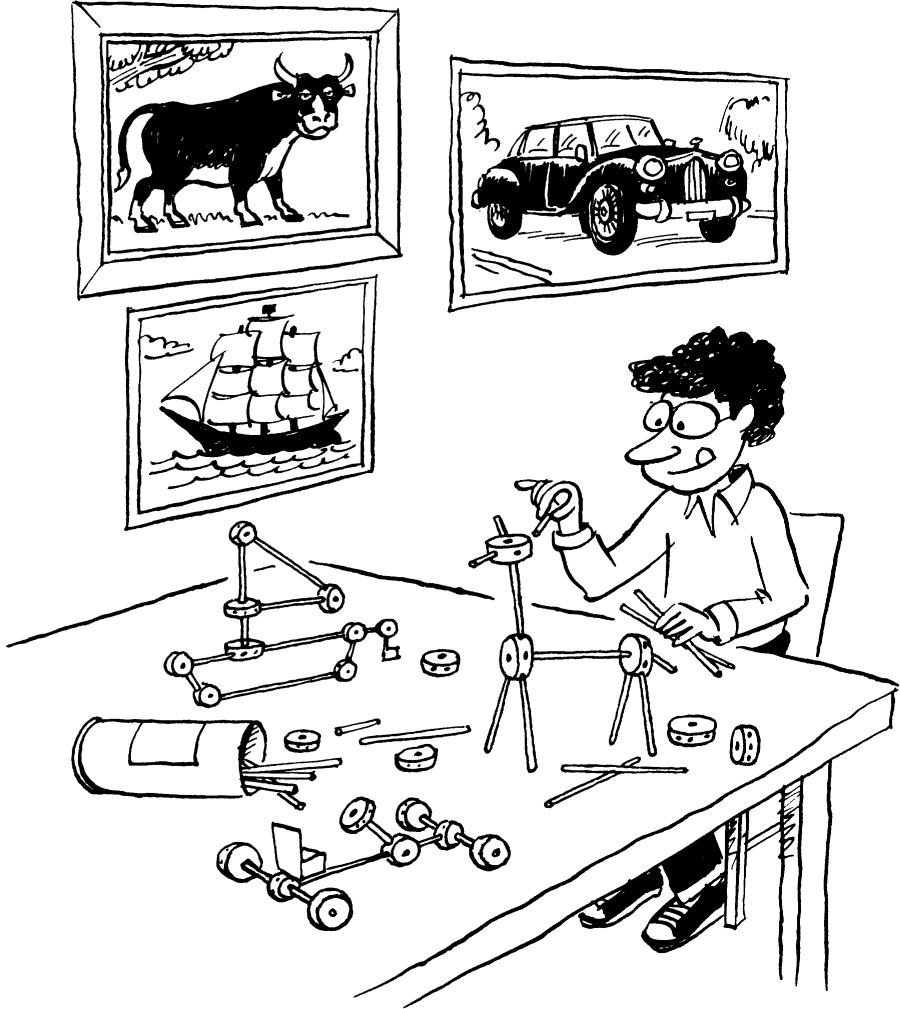
\includegraphics[width=0.5\textwidth]{deco_part1.jpg}

{\kaishu 插图：Dick Codor}
\end{center}

% 第1章 固体中的电子相互作用
\chapter{固体中的电子相互作用}

\section{单电子理论}

在周期势中运动的单个电子由能带结构方程描述：

\begin{equation*}
H ^ {0} \phi_ {\mathbf{k} s} (\mathbf{x}) \equiv \left[ - \frac {\hbar^ {2}}{2 m} \nabla^ {2} + V ^ {\mathrm{ion}} (\mathbf{x}) \right] \phi_ {\mathbf{k} s} (\mathbf{x}) = \epsilon_ {\mathbf{k}} \phi_ {\mathbf{k} s} (\mathbf{x}),
\tag{1.1}
\end{equation*}

其中 $\phi_{\mathbf{k}s}$ 与 $\epsilon_{\mathbf{k}}$ 分别是 Bloch 波函数和能带能量。$\mathbf{k}$ 是电子的格点动量，$s=\uparrow,\downarrow$ 是电子在 $S^{z}$ 方向的自旋。这里我们略去能带指标，并忽略自旋轨道耦合。

对 $N_{e}$ 个电子，只有当哈密顿量是单粒子哈密顿量的可分离求和时，Schrödinger 方程才能约化为一组能带结构方程 (1.1)：

\begin{equation*}
\mathcal {H} ^ {0} = \sum_ {i = 1} ^ {N _ {e}} H ^ {0} [ \nabla_ {i}, \mathbf {x} _ {i} ].
\tag{1.2}
\end{equation*}

(1.2) 的本征态是由 Slater 行列式构造的 Fock 态（见附录 A）：

\begin{equation*}
\Psi_ {[ \mathbf {k}, s ]} ^ {\mathrm{Fock}} (\mathbf {x} _ {1}, \dots , \mathbf {x} _ {N _ {e}}) = \det _ {ij} \left[ \phi_ {\mathbf {k} _ {i}, s _ {i}} (\mathbf {x} _ {j}) \right]
\tag{1.3}
\end{equation*}

本征能量为

\begin{equation*}
E _ {[ \mathbf {k} ]} = \sum_ {i = 1} ^ {N _ {e}} \epsilon_ {\mathbf {k} _ {i}}.
\tag{1.4}
\end{equation*}

在基态中最低的 $N_{e}$ 个态被占据，其最高能量称为费米能（Fermi energy）：

\begin{equation*}
\max \epsilon_ {\mathbf {k}} = \epsilon_ {F}.
\tag{1.5}
\end{equation*}

式 (1.5) 在 $\mathbf{k}$ 空间中定义了费米面（Fermi surface）。

包含电子间相互作用的哈密顿量是

\begin{equation*}
\mathcal {H} = \mathcal {H} ^ {0} + \frac {1}{2} \sum_ {i \neq j} v ^ {\mathrm{el-el}} (\mathbf {x} _ {i}, \mathbf {x} _ {j}).
\tag{1.6}
\end{equation*}

$v^{\mathrm{el-el}}$ 破坏了 (1.2) 的可分离性，使 $\mathcal{H}$ 的对角化比 $\mathcal{H}^0$ 困难得多。

通过修改离子势，可以把大部分 Coulomb 相互作用效应纳入 $H$ 的单粒子部分：

\begin{equation*}
\mathcal {H} ^ {0} \rightarrow \tilde {\mathcal {H}} ^ {0} = \sum_ {i = 1} ^ {N _ {e}} \left( H ^ {0} [ \nabla_ {i}, \mathbf {x} _ {i} ] + V ^ {\mathrm{ion}} (\mathbf {x} _ {i}) + v ^ {\mathrm{eff}} [ \mathbf {x} _ {i}, \rho ] \right),
\tag{1.7}
\end{equation*}

其中 $v^{\mathrm{eff}}$ 是基态密度 $\rho(\mathbf{x})$ 的泛函。文献中对 $v^{\mathrm{eff}}[\rho]$ 有各种近似方案（见文献注释）。对具体材料的多数能带结构计算都把 $v^{\mathrm{eff}}$ 取为局域的，即只依赖 $\mathbf{x}$ 处的 $\rho$（或许还有其空间导数）。而 $\rho$ 本身又通过求解 (1.7) 的基态自洽地确定。

剩余相互作用（residual interactions）为

\begin{equation*}
\tilde {v} _ {ij} = v ^ {\mathrm{el-el}} (\mathbf {x} _ {i}, \mathbf {x} _ {j}) - \left[ v ^ {\mathrm{eff}} (\mathbf {x} _ {i}) + v ^ {\mathrm{eff}} (\mathbf {x} _ {j}) \right] / N _ {e}.
\tag{1.8}
\end{equation*}

变换 $v^{\mathrm{el-el}} \to \tilde{v}$ 代表屏蔽（screening）。实际上，屏蔽是一个动力学过程，涉及以等离子体频率为尺度的集体电荷涨落。若等离子体频率高于所关心的激发能量，$\tilde{v}$ 可以取为瞬时的。在金属中，被屏蔽的相互作用在 Thomas--Fermi 屏蔽长度 $\lambda^{\mathrm{TF}}$ 内指数衰减。

忽略 $\tilde{v}_{ij}$ 的单电子近似方案，在预言许多材料的体能量与结构方面取得了巨大成功。然而，对于表现出磁性或超导电性的体系，剩余相互作用是决定性的。

$\tilde{v}_{ij}$ 的效应可以用 Feynman 图和时序 Green 函数做微扰计算。对某些图类的重新求和（如随机相位近似中的做法）可用于描述无相互作用体系向有序基态的不稳定性。这些方法在许多教科书中都有详细论述，其中一部分列于本章文献注释。本书要强调的技术，是专门为补充微扰论、处理强电子--电子相互作用而设计的。

\section{场与相互作用}

在多电子 Hilbert 空间中，使用强制实现所有态反对称性的二次量子化算符是方便的（见附录 A）。场算符 $\psi_{s}^{\dagger}(\mathbf{x})$ 产生一个局域在 $\mathbf{x}$ 处、自旋态为 $s$ 的粒子：

\begin{equation*}
\langle \mathbf {x} ' s ' | \psi_ {s} ^ {\dagger} (\mathbf {x}) | 0 \rangle = \delta_ {ss'} \delta (\mathbf {x} - \mathbf {x} ').
\tag{1.9}
\end{equation*}

利用 (A.10)，可以用任何正交归一的单粒子基底 $\{\phi\}$ 展开场算符：

\begin{equation*}
\psi_ {s} ^ {\dagger} (\mathbf {x}) = \sum_ {i} \phi_ {i} ^ {*} (\mathbf {x}) c _ {is} ^ {\dagger},
\tag{1.10}
\end{equation*}

其中 $c^{\dagger}, c$ 是反对易的产生与湮灭算符。于是场算符满足

\begin{equation*}
\{ \psi_ {s} ^ {\dagger} (\mathbf {x}), \psi_ {s '} (\mathbf {x} ') \} = \delta (\mathbf {x} - \mathbf {x} ') \delta_ {ss'}.
\tag{1.11}
\end{equation*}

局域密度算符定义为

\begin{align*}
\hat {\rho} (\mathbf {x}) & = \sum_ {s} \psi_ {s} ^ {\dagger} (\mathbf {x}) \psi_ {s} (\mathbf {x})
\tag{1.12}\\
& = \sum_ {ii's} \phi_ {i} ^ {*} (\mathbf {x}) \phi_ {i '} (\mathbf {x}) c _ {is} ^ {\dagger} c _ {i's}.
\tag{1.13}
\end{align*}

$\hat{\rho}$ 度量在 $\mathbf{x}$ 处找到任一自旋粒子的概率密度。注意局域密度算符一般含有非对角项 $i \neq i'$。$\hat{\rho}(\mathbf{x})$ 是 Schrödinger 密度算符的二次量子化表示，后者在坐标空间中的期望值为

\begin{equation*}
\rho (\mathbf {x}) = \sum_ {i} \delta (\mathbf {x} - \mathbf {x} _ {i}).
\tag{1.14}
\end{equation*}

由 $|x_{1}, x_{2}, \ldots\rangle$ 规定的 Fock 态是 $\hat{\rho}(\mathbf{x})$ 的本征态，本征值为 $\rho(\mathbf{x})$。因此，用局域场算符与密度算符 (1.10) 和 (1.13) 来表示局域算符 $H$ 是自然的。像 (1.7) 与 (1.8) 那样把单粒子部分与剩余相互作用部分分开，我们写

\begin{equation*}
\mathcal {H} = \tilde {\mathcal {H}} ^ {0} + \tilde {\mathcal {V}} ^ {\mathrm{el-el}},
\tag{1.15}
\end{equation*}

其中

\begin{equation*}
\tilde {\mathcal {H}} ^ {0} = \sum_ {s} \int d ^ {3} x \, \psi_ {s} ^ {\dagger} (\mathbf {x}) \left[ - \frac {\hbar^ {2}}{2 m} \nabla^ {2} + V ^ {\mathrm{ion}} + v ^ {\mathrm{eff}} (\mathbf {x}) \right] \psi_ {s} (\mathbf {x}),
\tag{1.16}
\end{equation*}

以及

\begin{align*}
\tilde {\mathcal {V}} ^ {\mathrm{el-el}} & = \frac {1}{2} \int d ^ {3} x \, d ^ {3} y \, \tilde {v} (\mathbf {x}, \mathbf {y}) \left[ \hat {\rho} (\mathbf {x}) \hat {\rho} (\mathbf {y}) - \delta (\mathbf {x} - \mathbf {y}) \hat {\rho} (\mathbf {x}) \right]
\tag{1.17}\\
& = \frac {1}{2} \int d ^ {3} x \, d ^ {3} y \, \tilde {v} (\mathbf {x}, \mathbf {y}) \sum_ {ss'} \psi_ {s} ^ {\dagger} (\mathbf {x}) \psi_ {s '} ^ {\dagger} (\mathbf {y}) \psi_ {s '} (\mathbf {y}) \psi_ {s} (\mathbf {x}).
\end{align*}

在 (1.17) 的第二行中，场算符已正规排序，这消除了自相互作用项 $\tilde{v}(0)\,\delta(\mathbf{x}-\mathbf{y})\hat{\rho}$。

\begin{figure}[H]
\centering
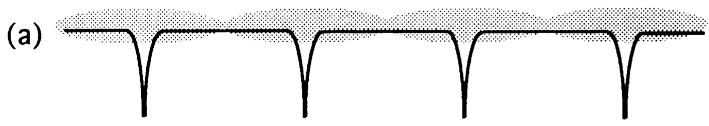
\includegraphics[width=0.86\textwidth]{fig1_1a.jpg}\\[2pt]
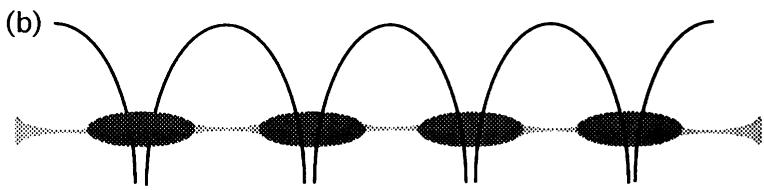
\includegraphics[width=0.86\textwidth]{fig1_1b.jpg}
\caption{传导电子密度：(a)~$s$、$p$ 电子；(b)~$d$、$f$ 电子。实线是有效离子势。}
\label{fig:1.1}
\end{figure}

\section{金属中相互作用的量级}

必须强调，先验地判定一个给定体系中的剩余相互作用应当算“弱”还是“强”并不容易。恰当的问法是：它们对基态关联和低能激发的影响是否剧烈。微扰论可以作为估计相互作用效应的指南。粗略地说，金属中 Coulomb 相互作用效应的无量纲参数是

\begin{equation*}
g = \frac {e ^ {2}}{\kappa \epsilon_ {F} \left\langle r _ {ij} \right\rangle}
\tag{1.18}
\end{equation*}

其中 $e$ 是电子电荷，$\kappa$ 是静态介电常数，$\langle r_{ij}\rangle$ 是电子间平均距离，$\epsilon_{F}$ 是从导带底算起的费米能。贡献传导电子的离子在元素周期表中的位置越靠下，相对相互作用强度越大。离子势对 $s$、$p$ 传导电子的作用较弱，因此导带波函数是离域的，密度在整个晶体中相当均匀，如图~\ref{fig:1.1}(a) 所示。其结果是电子间相互作用相对较弱。

相反，过渡金属和混合价稀土化合物向导带贡献 $d$、$f$ 电子。在那里，电子大部分局域在围绕离子、半径 $\langle r_{ij}\rangle \ll a$ 的小区域内，$a$ 是晶格间距。同时，如图~\ref{fig:1.1}(b) 所示，大的原子间势垒压低了费米能 $\epsilon_{F}$。于是可以预期，过渡金属和混合价稀土化合物的 $g$ 值很大，应视为强相互作用电子体系。

这种分类只是粗略的经验法则。它无法预言某个具体化合物是顺磁金属，还是具有磁有序、电荷密度波或超导序。显然，无相互作用的简并基态对解除简并的微扰极为敏感。因此基态灵敏地依赖于能带结构的细节以及 $\tilde{H}^{0}$ 中的近简并。

\section{有效模型}

$\tilde{V}^{\mathrm{el-el}}$ 中的四费米子相互作用使 $H$ 成为真正的多体问题，因而极难对角化。数值方法只限于非常小的体系，因为 Hilbert 空间的维数随电子数目和单粒子基底的大小指数增长。理论家们于是求助于简化的模型（见第一部分扉页插图），其中只保留一个约减的单粒子态集合和相互作用矩阵元。

把 $H$ 替换为有效模型，若表述为重整化群变换\footnote{可参看 Shankar 的综述。}，则可以建立在更稳固的基础上。当人们关心低频、低温关联时，可以把 Green 函数投影到低能部分，从而消去高能态，得到一个只在低能子空间中作用的有效哈密顿量 $H^{\mathrm{eff}}$\footnote{例如：3.2 节中 t--J 模型就是作为大 $U$ Hubbard 模型的有效哈密顿量导出的。}。在路径积分表述中，可以把高频模式积掉，留下低频模式的有效 Lagrange 量\footnote{例如参看第 13 章中非线性 $\sigma$ 模型的重整化。}。

变换 $H \rightarrow H^{\mathrm{eff}}$ 称为重整化（renormalization）。在重整化下，某些相互作用（称为无关的，irrelevant）相对于其他相互作用被压低；增长或保持不变的分别被称为有关的（relevant）或边缘的（marginal）。这样，能带结构和相互作用的许多微观细节都从有效哈密顿量中消失，后者只包含最有关的相互作用。如果重整化得到一个单粒子态更少、相互作用更简化的模型，那么求低能关联就大有希望。有效模型的参数原则上可以通过求解重整化群流从微观哈密顿量确定。诚然，对真实材料的这类计算很少完成过，模型参数通常是拟合实验确定的。在缺乏可靠计算的情况下，某些相互作用无关还是有关，成了不同模型的支持者之间悬而未决的争论根源。

相互作用电子的一个最小模型是 Hubbard 模型，将在第 3 章描述。然而，即使是 Hubbard 模型也只在一维情形被严格求解。一个更简单、但仍包含多体相互作用的模型是量子 Heisenberg 模型，它将在第 3 章中作为 Hubbard 模型的一个特殊极限导出。虽然它只描述自旋自由度，但其基态和激发是高度关联的（即远非少数几个 Fock 态的组合）。Heisenberg 模型丰富的物理性质统称“量子磁性”（Quantum Magnetism），这是本书的主题之一。我们将用相当的篇幅讨论自旋相互作用及其对量子涨落和热涨落的影响。在更宽的视野里，量子 Heisenberg 模型将被用来演示基本的物理概念；作为一种教学工具，我们将在它上面检验各种对其他量子多粒子体系同样适用的数学技巧和近似方案。

\begin{exercises}

\item 利用附录 A 的 (A.24)，求自由玻色子和自由费米子的总粒子数 $N = -\partial F/\partial \mu$、熵 $S = -\partial F/\partial T$ 和比热 $C_{v} = T \,\partial S/\partial T$。

\end{exercises}

\begin{chapbib}
\item 关于固体电子结构的一般背景有大量优秀教科书，例如：
  N. W. Ashcroft and N. D. Mermin, \textit{Solid State Physics} (Holt, Rinehart, and Winston, 1976)；
  C. Kittel, \textit{Quantum Theory of Solids} (John Wiley and Sons, 1987)；
  J. Callaway, \textit{Quantum Theory of the Solid State} (Academic Press, 1992)；
  W. Jones and N. H. March, \textit{Theoretical Solid State Physics} (Dover, 1973)。
\item 凝聚态多体图微扰论的基本技术可参看，例如：
  A. Fetter and J. D. Walecka, \textit{Quantum Theory of Many Particle Systems} (McGraw-Hill, 1971)；
  G. Mahan, \textit{Many Particle Physics} (Plenum Press, 1981)。
\item P. Fulde, \textit{Electron Correlations in Molecules and Solids} (Springer-Verlag, 1991)。
  这本新著也值得推荐为当代理论与实验参考书。
\item 建议的进一步背景阅读：
  P. W. Anderson, \textit{Concepts in Solids} (Addison-Wesley, 1963)。
\item 关于相互作用电子重整化群的一篇出色新近教程：
  R. Shankar, Rev. Mod. Phys. \textbf{66}, 129 (1994)。
\item 关于相互作用电子的场论方法，两部著名的教科书是：
  E. Fradkin, \textit{Field Theories of Condensed Matter Systems} (Addison-Wesley, 1991)；
  A. M. Tsvelik, \textit{Quantum Field Theory in Condensed Matter Physics} (Cambridge University Press, 1995)。
\end{chapbib}

% 第2章 自旋交换
\chapter{自旋交换}

当固体中许多电子的磁矩排成一致时，便出现铁磁性。反铁磁性和自旋密度波描述磁矩的振荡式排列。电子磁矩之间的经典偶极相互作用（量级 $10^{-5}$~eV）远远不足以解释观测到的磁转变温度（过渡金属和稀土化合物中量级为 $10^{2}\text{--}10^{3}$~K）。因此，量子力学发展初期人们就认识到，产生磁性的耦合机制来源于电子的如下基本性质：

\begin{enumerate}[itemsep=1pt]
\item 电子的自旋；
\item 电子的动能（离域化能量）；
\item Pauli 不相容原理（Fermi 统计）；
\item 电子间的 Coulomb 排斥。
\end{enumerate}

作为入门例子，我们研究两个被外势束缚在空间局域位置、并通过 Coulomb 相互作用彼此排斥的电子。我们将发现，两个电子自旋之间的耦合既可以是铁磁的，也可以是反铁磁的，取决于无相互作用态的性质。这些正是相互作用电子体系得以产生各种磁结构的基本机制。

\section{铁磁交换}

考虑两个电子，占据两个近简并的单粒子轨道 $\phi_{1}$、$\phi_{2}$，能量分别为 $\epsilon_{1}$、$\epsilon_{2}$。我们假设谱的其余部分与这两个态之间隔着一个大能隙。图~\ref{fig:2.1} 画出了这类态的一维例子。实际上，它们可以是一个原子或分子的低角动量多重态的成员。我们还假设有两个电子，可以占据其中任一个或两个态。不同组态的简并被 Coulomb 相互作用解除。我们把电子场算符在 $\phi_{i}$ 基组中展开为

\begin{equation*}
\psi_ {s} ^ {\dagger} (x) = \sum_ {i = 1} ^ {2} \phi_ {i} ^ {*} c _ {is} ^ {\dagger}, \quad s = \uparrow , \downarrow
\tag{2.1}
\end{equation*}

\begin{figure}[H]
\centering
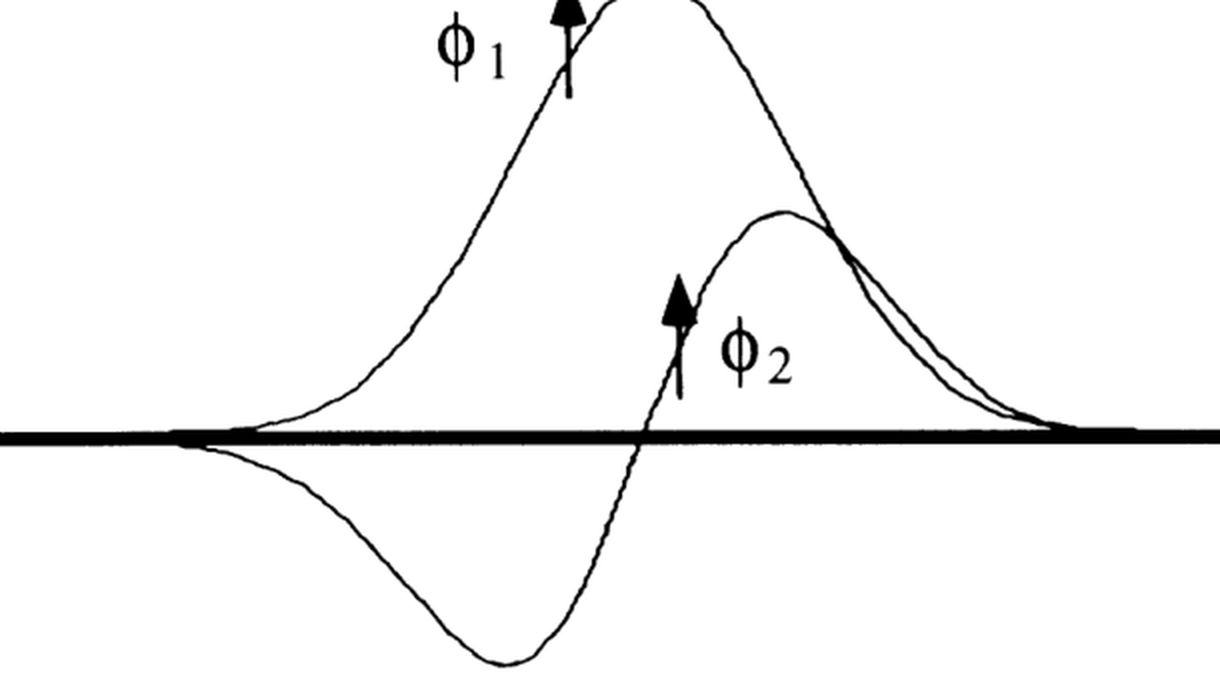
\includegraphics[width=0.62\textwidth]{fig2_1_scan.png}
\caption{彼此铁磁耦合的两个电子的态。}
\label{fig:2.1}
\end{figure}

二次量子化形式下的两体 Coulomb 相互作用由（见 (1.17)）

\begin{equation*}
\mathcal {V} = \frac {1}{2} \int d ^ {3} x \, d ^ {3} y \, \tilde {v} (\mathbf {x}, \mathbf {y}) \sum_ {ss'} \psi_ {s} ^ {\dagger} (\mathbf {x}) \psi_ {s '} ^ {\dagger} (\mathbf {y}) \psi_ {s '} (\mathbf {y}) \psi_ {s} (\mathbf {x})
\tag{2.2}
\end{equation*}

给出。用 (2.1) 把 (2.2) 写到 $i$ 表象中：

\begin{equation*}
\mathcal {V} = \sum_ {i \neq i'} U _ {ii'} n _ {i} n _ {i'} + \sum_ {i} U _ {ii} \rho_ {i \uparrow} \rho_ {i \downarrow} + \sum_ {ss',\, i \neq i'} J ^ {F} c _ {is} ^ {\dagger} c _ {i's'} ^ {\dagger} c _ {is'} c _ {i's},
\tag{2.3}
\end{equation*}

其中 $n_i = \sum_s \rho_{is}$。相互作用参数由\emph{直接}积分给出：

\begin{equation*}
U _ {ii'} = \frac {1}{2} \int d ^ {3} x \, d ^ {3} y \, \tilde {v} (\mathbf {x}, \mathbf {y}) \, | \phi_ {i} (\mathbf {x}) | ^ {2} \, | \phi_ {i'} (\mathbf {y}) | ^ {2}
\tag{2.4}
\end{equation*}

以及\emph{铁磁交换}常数：

\begin{equation*}
J ^ {F} = \frac {1}{2} \int d ^ {3} x \, d ^ {3} y \, \tilde {v} (\mathbf {x}, \mathbf {y}) \, \phi_ {i} (\mathbf {x}) \phi_ {i'} ^ {*} (\mathbf {x}) \phi_ {i'} (\mathbf {y}) \phi_ {i} ^ {*} (\mathbf {y}).
\tag{2.5}
\end{equation*}

容易看出 $U_{ii'}$ 为正，$J^{F}$ 为实。显然，对短程相互作用 $\tilde{v} = \delta(\mathbf{x} - \mathbf{y})$，有 $J^{F} > 0$。对长程 Coulomb 相互作用 $v^{c} = e^{2}/|\mathbf{x} - \mathbf{y}|$，$J^{F}$ 的正性证明如下。对称算符 $v^{c}(\mathbf{x}, \mathbf{y})$ 的本征值为

\begin{equation*}
\int d ^ {3} x \, e ^ {i \mathbf {kx}} \frac {e ^ {2}}{| \mathbf {x} |} = \frac {4 \pi e ^ {2}}{\mathbf {k} ^ {2}} > 0.
\tag{2.6}
\end{equation*}

因此 $v^{c}$ 的一切期望值都为正，特别是在态 $\Phi(\mathbf{x}) = \phi_{i'}^{*}\phi_{i}$ 中的期望值，即 (2.5) 为正。这样我们证明了 (2.5) 在两种极限情形下均为正：(i) 完全屏蔽，(ii) 完全无屏蔽。

现在，若

\begin{equation*}
\epsilon_ {1} + \epsilon_ {2} + U _ {12} < \min \left[ 2 \epsilon_ {1} + U _ {11}, \; 2 \epsilon_ {2} + U _ {22} \right],
\tag{2.7}
\end{equation*}

则基态主要含有占据不同轨道的两个电子，即 $n_{i} \approx 1$，低能态由

\begin{equation*}
\left\{ \left| s _ {1}, s _ {2} \right\rangle \right\} , \quad s _ {i} = \uparrow , \downarrow
\tag{2.8}
\end{equation*}

给出。交换相互作用 $J^{F}$ 在 (2.8) 空间中表现为 Heisenberg 相互作用：

\begin{equation*}
J ^ {F} \sum_ {ss'} c _ {is} ^ {\dagger} c _ {i's'} ^ {\dagger} c _ {is'} c _ {i's} = - 2 J ^ {F} \left( \mathbf {S} _ {i} \cdot \mathbf {S} _ {i'} + \frac {1}{4} n _ {i} n _ {i'} \right).
\tag{2.9}
\end{equation*}

$\mathbf{S}_i^\alpha$（$\alpha = x, y, z$）是自旋 $1/2$ 算符的分量（见 (A.19)）：

\begin{equation*}
\mathbf {S} _ {i} \equiv \frac {1}{2} \sum_ {ss'} c _ {is} ^ {\dagger} \vec {\sigma} _ {ss'} c _ {is'}.
\tag{2.10}
\end{equation*}

交换积分 (2.5) 依赖轨道间的空间交叠。(2.3) 与 (2.9) 显式地展示了占据这类轨道的电子自旋之间的铁磁耦合。

一个物理论证：各自旋彼此平行排列、构成对称自旋态后，会削弱 Coulomb 排斥的效应。此时两电子态是反对称的，因而其轨道波函数必须在 $\mathbf{x} - \mathbf{y} = 0$ 处为零——那里正是 Coulomb 势最大的地方。

这一效应出现在微扰论的一阶，与原子中 Hund 定则背后的物理相同：开壳层中的电子占据轨道时使总自旋最大化\footnote{第二 Hund 定则说，第一定则中的含糊之处通过使总轨道角动量最大化来解决。}。

\section{反铁磁交换}

展示两个电子间反铁磁耦合的最简单体系是 $H_{2}$ 分子，最早由 Heitler 和 London 讨论\footnote{这里的讨论相当紧随 Mattis 的书。}。

把两个质子冻结在平衡位置 $R_{i}$，记电子坐标为 $x_{i}$（$i = 1, 2$）。完整哈密顿量为

\begin{equation*}
H = \sum_ {i = 1} ^ {2} H _ {i} ^ {\infty} + \Delta H,
\tag{2.11}
\end{equation*}

\begin{figure}[H]
\centering
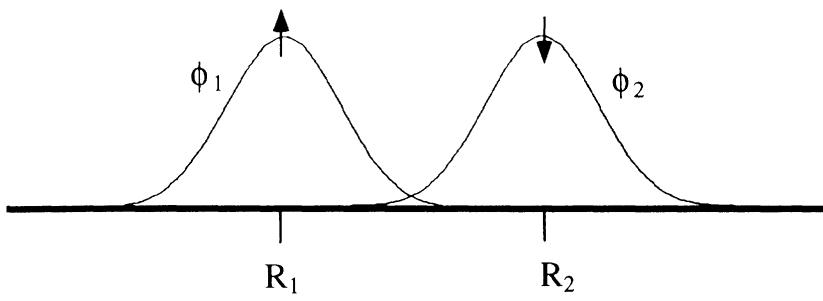
\includegraphics[width=0.55\textwidth]{fig2_2.jpg}
\caption{彼此反铁磁耦合的两个电子的态。}
\label{fig:2.2}
\end{figure}

\begin{align*}
H _ {i} ^ {\infty} & = - \frac {\hbar^ {2}}{2 m} \nabla_ {i} ^ {2} - \frac {e ^ {2}}{| \mathbf {x} _ {i} - \mathbf {R} _ {i} |},\\
\Delta H & = - \sum_ {i \neq j} \frac {e ^ {2}}{| \mathbf {x} _ {i} - \mathbf {R} _ {j} |} + \frac {e ^ {2}}{| \mathbf {x} _ {1} - \mathbf {x} _ {2} |} + \frac {e ^ {2}}{| \mathbf {R} _ {1} - \mathbf {R} _ {2} |}.
\tag{2.12}
\end{align*}

两个原子波函数 $\phi_{1}$、$\phi_{2}$ 分别以原子 1、2 为中心，如图~\ref{fig:2.2} 所示。它们满足原子 Schrödinger 方程：

\begin{equation*}
H _ {i} ^ {\infty} \phi_ {i} (\mathbf {x} _ {i}) = e _ {0} \phi_ {i} (\mathbf {x} _ {i}), \quad i = 1, 2.
\tag{2.13}
\end{equation*}

当原子间距有限，$|R_{1}-R_{2}|<\infty$ 时，$\phi_{1}$ 与 $\phi_{2}$ 不正交，其交叠为

\begin{equation*}
\lambda = \int d ^ {3} x \, \phi_ {1} ^ {*} (\mathbf {x}) \phi_ {2} (\mathbf {x}).
\tag{2.14}
\end{equation*}

用 $\phi_{i}$ 构造轨道波函数

\begin{align*}
\psi^ {a} & = \phi_ {1} (\mathbf {x} _ {1}) \phi_ {2} (\mathbf {x} _ {2}),\\
\psi^ {b} & = \phi_ {1} (\mathbf {x} _ {2}) \phi_ {2} (\mathbf {x} _ {1}).
\tag{2.15}
\end{align*}

(2.15) 描述处于不同格点上的电子。我们可用它们构造变分波函数 $\Psi$，以避免大的在位 Coulomb 排斥（稍后我们将用波函数的自旋部分 $\chi$ 施加反对称约束）：

\begin{equation*}
\Psi = \left( c ^ {a} \psi^ {a} + c ^ {b} \psi^ {b} \right) \chi.
\tag{2.16}
\end{equation*}

变分能量为

\begin{equation*}
E = \langle \Psi | H | \Psi \rangle / \langle \Psi | \Psi \rangle.
\tag{2.17}
\end{equation*}

对 $c^a, c^b$ 极小化 $E[c^a, c^b]$，得到矩阵方程：

\begin{equation*}
\left[ \left( \begin{array}{cc} U ^ {d} & U ^ {o} \\ (U ^ {o}) ^ {*} & U ^ {d} \end{array} \right) - (E - 2 e _ {0}) \left( \begin{array}{cc} 1 & \lambda^ {2} \\ \lambda^ {*2} & 1 \end{array} \right) \right] \binom{c ^ {a}}{c ^ {b}} = 0,
\tag{2.18}
\end{equation*}

其中

\begin{equation*}
U ^ {d} = \int d ^ {3} x _ {1} \, d ^ {3} x _ {2} \; \Delta H \, | \psi^ {a} | ^ {2},
\tag{2.19}
\end{equation*}

\begin{equation*}
U ^ {o} = \int d ^ {3} x _ {1} \, d ^ {3} x _ {2} \; \Delta H \, (\psi^ {a}) ^ {*} \psi^ {b}
\tag{2.20}
\end{equation*}

是对角与非对角项。由于 $\psi^{a}$、$\psi^{b}$ 可以取为实（它们由氢原子基态构成），$\lambda$ 与 $U^{o}$ 也可取为实。(2.18) 的解为

\begin{equation*}
E ^ {\pm} = 2 e _ {0} + \frac {U ^ {d} \pm U ^ {o}}{1 \pm \lambda^ {2}},
\tag{2.21}
\end{equation*}

\begin{equation*}
\binom{c ^ {a}}{c ^ {b}} ^ {\pm} = \frac {1}{\sqrt {2}} \binom{1}{\mp 1}.
\tag{2.22}
\end{equation*}

现在施加反对称条件：$\Psi$ 与波函数自旋部分 $\chi(\mathbf{x}_{1},\mathbf{x}_{2})$ 的乘积必须对交换电子坐标反对称：

\begin{align*}
\Psi^ {\pm} & = \frac {1}{\sqrt {2}} \left( \psi^ {a} \mp \psi^ {b} \right) \chi^ {\pm}\\
& = \frac {1}{\sqrt {2}} \left[ \phi_ {1} (\mathbf {x} _ {1}) \phi_ {2} (\mathbf {x} _ {2}) \mp \phi_ {1} (\mathbf {x} _ {2}) \phi_ {2} (\mathbf {x} _ {1}) \right] \chi^ {\pm},\\
\chi^ {\pm} & = \frac {1}{\sqrt {2}} \left[ \chi^ {\uparrow} (\mathbf {x} _ {1}) \chi^ {\downarrow} (\mathbf {x} _ {2}) \pm \chi^ {\uparrow} (\mathbf {x} _ {2}) \chi^ {\downarrow} (\mathbf {x} _ {1}) \right],
\tag{2.23}
\end{align*}

其中 $\chi^{\pm}$ 描述反平行自旋。容易验证 $\Psi^{\pm}$ 是两个 Slater 行列式的线性组合，每个行列式都可写成一个 Fock 态\footnote{严格地说，为了把它们定义为 Fock 态，必须先把 $\phi_{1}$、$\phi_{2}$ 正交化。}。于是，用二次量子化记号可以写

\begin{equation*}
\Psi^ {\pm} = \frac {1}{\sqrt {2}} \left( c _ {1 \uparrow} ^ {\dagger} c _ {2 \downarrow} ^ {\dagger} \pm c _ {1 \downarrow} ^ {\dagger} c _ {2 \uparrow} ^ {\dagger} \right) | 0 \rangle .
\tag{2.24}
\end{equation*}

由这一形式显而易见，$\Psi^{-}$ 与 $\Psi^{+}$ 正是总自旋算符

\begin{equation*}
\mathbf {S} ^ {\mathrm{tot}} = \sum_ {i = 1} ^ {2} \frac {1}{2} \sum_ {ss'} c _ {is} ^ {\dagger} \vec {\sigma} _ {ss'} c _ {is'}
\tag{2.25}
\end{equation*}

的三重态和单态本征态。单态与三重态的劈裂为

\begin{align*}
E ^ {+} - E ^ {-} & = J\\
J & = 2 \, \frac {U ^ {d} \lambda^ {2} - U ^ {o}}{1 - \lambda^ {4}}.
\tag{2.26}
\end{align*}

通过显式计算参数 $U^{d}$ 与 $U^{o}$ 可以证明，对所有 $R_{12}$，$J$ 为正（反铁磁）。因此基态是单态，较高态是三重态，有效哈密顿量可以用 Heisenberg 反铁磁体表示：

\begin{align*}
\mathcal {H} ^ {\mathrm{QHM}} & = + J \, \mathbf {S} _ {1} \cdot \mathbf {S} _ {2}\\
& = J \left[ \frac {1}{2} (\mathbf {S} ^ {\mathrm{tot}}) ^ {2} - \frac {3}{4} \right] = \left\{ \begin{array}{ll} \frac {1}{4} J & S^{\mathrm{tot}} = 1 \\[2pt] - \frac {3}{4} J & S^{\mathrm{tot}} = 0 \end{array} \right. .
\tag{2.27}
\end{align*}

物理论证：反平行的自旋可以利用杂化，在另一个电子占据该格点的同时跳跃过去，从而降低动能。平行自旋则被 Pauli 原理禁止进行这种虚过程，这使三重态能量高于单态。

小结：当两个电子局域在能量相近的轨道上并有排斥相互作用时，它们的磁耦合为：

\begin{enumerate}[itemsep=1pt]
\item \textbf{铁磁}：若两轨道正交但占据空间的同一区域。此时自旋平行排列降低相互作用能。
\item \textbf{反铁磁}：若两轨道不正交但在空间上分离。此时自旋反平行排列降低动能。
\end{enumerate}

\section{超交换}

上一节我们看到，近邻氢原子上的两个电子由于在位排斥与离域能量的相互抗争而倾向于反铁磁耦合。用二次量子化算符，把能量按跳跃矩阵元展开到二阶，可以简单地导出这一效应。考虑局域在两个原子（标记 $i = 1, 2$）上的两个正交轨道。两态之间的隧穿由跳跃哈密顿量描述：

\begin{equation*}
\mathcal {H} ^ {t} = - t \sum_ {s} \left( c _ {1s} ^ {\dagger} c _ {2s} + c _ {2s} ^ {\dagger} c _ {1s} \right).
\tag{2.28}
\end{equation*}

为简单起见，取在位（Hubbard）相互作用：

\begin{equation*}
\mathcal {U} = U \sum_ {i} n _ {i \uparrow} n _ {i \downarrow}.
\tag{2.29}
\end{equation*}

对大的 $U/t$，取 $\mathcal{U}$ 为零级哈密顿量，其基态流形是四重简并的：

\begin{equation*}
\{0 \} = \left| s _ {1}, s _ {2} \right\rangle , \quad s _ {i} = \uparrow , \downarrow, \; i = 1, 2.
\tag{2.30}
\end{equation*}

双占据轨道的能量比多重态 (2.30) 高 $U$。$\mathcal{H}^t$ 的一阶微扰会把我们带出基态流形，因为它把一个电子放到另一个上面。在子空间 (2.30) 内做二阶微扰，得到由标准表达式\footnote{参看 Landau 与 Lifshitz，见本章文献注释。}给出的有效哈密顿量

\begin{equation*}
\langle a | \mathcal {H} ^ {(2)} | b \rangle = - \left\langle a \left| \mathcal {H} ^ {t} \frac {1 - P _ {0}}{\mathcal {U}} \mathcal {H} ^ {t} \right| b \right\rangle = - \sum_ {n \not\in \{0 \}} \langle a | \mathcal {H} ^ {t} | n \rangle \, \frac {1}{\langle n | \mathcal {U} | n \rangle} \, \langle n | \mathcal {H} ^ {t} | b \rangle ,
\tag{2.31}
\end{equation*}

其中 $a, b$ 是子空间 $\{0\}$ 中的态，$P_{0}$ 是其投影算符，而 $|n\rangle$ 含有双占据。和式中的每一项都可以用一条“交换路径”表示。例如

\begin{equation*}
\begin{array}{ccccc}
 & \mathcal {H} ^ {t} & \ \ \frac {1}{\mathcal {U}}\ \ & & \mathcal {H} ^ {t} \\
| \uparrow , \downarrow \rangle & \to & | \uparrow \downarrow , 0 \rangle & \to & | \downarrow , \uparrow \rangle \\
 & & \to & | 0, \uparrow \downarrow \rangle & \to\ | \downarrow , \uparrow \rangle .
\end{array}
\tag{2.32}
\end{equation*}

(2.32) 中两条路径各给出贡献 $-t^{2}/U$。但也存在被 Pauli 不相容原理阻塞的路径，例如

\begin{equation*}
\begin{array}{ccc}
 & \mathcal {H} ^ {t} & \\
| \uparrow , \uparrow \rangle & \to & 0.
\end{array}
\tag{2.33}
\end{equation*}

因此三重态不能靠虚双占获得二阶能量增益。连接这些初末态的算符可以写成 $S=\tfrac{1}{2}$ 自旋算符的乘积 $S_{1}^{-}S_{2}^{+}$。把描述 $S_{2}^{-}S_{1}^{+}$ 与 $S_{1}^{z}S_{2}^{z}$ 矩阵元的路径也包括进来，我们发现基态子空间中的有效哈密顿量可写成各向同性的反铁磁 Heisenberg 交换：

\begin{equation*}
\mathcal {H} ^ {(2)} = J \, \mathbf {S} _ {1} \cdot \mathbf {S} _ {2} \, , \quad J = \frac {4 t ^ {2}}{U}.
\tag{2.34}
\end{equation*}

这一讨论容易推广到多格点体系：任何两个由跳跃项 $H^{t}$ 耦合的自旋之间都会产生反铁磁耦合。

虚双占据过程称为“\textbf{超交换}”（superexchange）。上一节对氢分子的分析用变分方法描述了同一效应。我们要把超交换与 2.1 节讲的铁磁直接交换或 Hund 定则区分开：后者是相互作用一阶微扰的结果\footnote{Anderson 在其原始论文（见文献注释）中考虑了几种交换机制。在那里，“超交换”专指经过一个中间离子的耦合。}。

\begin{figure}[H]
\centering
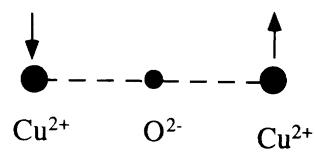
\includegraphics[width=0.5\textwidth]{fig2_3a.jpg}\\[4pt]
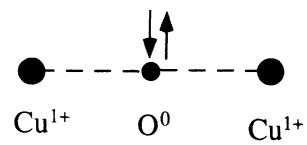
\includegraphics[width=0.5\textwidth]{fig2_3b.jpg}
\caption{铜氧化物中的超交换。(a)~低能流形的一个成员；(b)~超交换路径中的一个高能组态。}
\label{fig:2.3}
\end{figure}

超交换耦合在许多其他带有未配对自旋的体系中产生。当前备受关注的著名例子是铜氧化物反铁磁体。未配对自旋位于 $Cu^{2+}$ 离子上，二者之间有一个氧“桥”离子，平均电离态接近 $O^{2-}$。这样的三原子组合见图~\ref{fig:2.3}。

若铜与氧之间没有跳跃，则键上的简并基态流形为

\begin{equation*}
\{ | 0 \rangle \} = \left\{ \left| \mathrm{Cu} ^ {2+} s _ {1}, \mathrm{O} ^ {2-}, \mathrm{Cu} ^ {2+} s _ {2} \right\rangle , \quad s _ {i} = \uparrow , \downarrow \right\}
\tag{2.35}
\end{equation*}

解除 (2.35) 简并的基态能量的最低阶修正是铜--氧跳跃的四阶项。超交换路径的中间态及其能量的例子有

\begin{equation*}
\left| \mathrm{Cu} ^ {1+}, \mathrm{O} ^ {2-}, \mathrm{Cu} ^ {3+} \uparrow \downarrow \right\rangle , \quad E = U _ {d},
\tag{2.36}
\end{equation*}

以及另一个具有不同能量分母的态

\begin{equation*}
\left| \mathrm{Cu} ^ {1+}, \mathrm{O} \uparrow \downarrow , \mathrm{Cu} ^ {1+} \right\rangle , \quad E = 2 (\epsilon_ {p} - \epsilon_ {d}) + U _ {p},
\tag{2.37}
\end{equation*}

其中 $\epsilon_{d(p)}$ 与 $U_{d(p)}$ 分别是铜（氧）上的单粒子能量和相互作用能。如 (2.33) 所示，平行自旋态被阻挡，无法跳跃进入这两个中间态中的任何一个。这就解除了 (2.35) 中单态与三重态的简并，简并的解除由 Heisenberg 哈密顿量描述。反铁磁耦合由对所有超交换路径求和给出，因此由能量最低的中间态主导。

\begin{exercises}

\item 自旋算符的费米子表示由 (2.10) 给出。证明重要恒等式 (2.9)：

\begin{equation*}
\sum_ {ss'} c _ {1s} ^ {\dagger} c _ {2s'} ^ {\dagger} c _ {1s'} c _ {2s} = - \frac {1}{2} \left\{ n _ {1} n _ {2} + 4 \, \mathbf {S} _ {1} \cdot \mathbf {S} _ {2} \right\},
\tag{2.38}
\end{equation*}

其中 $n_i = \sum_s c_{is}^\dagger c_{is}$，$i = 1,2$。

\item 证明 $\mathbf{S}_i$ 满足角动量对易关系。求 $\mathbf{S}_i^2$ 作为 $n_i$ 函数的简单表达式。

\end{exercises}

\begin{chapbib}
\item 氢分子的分析相当紧随 Mattis 的书：
  D. C. Mattis, \textit{The Theory of Magnetism I} (Springer-Verlag, 1988)。
\item 超交换理论由 Kramers 提出，并由 Anderson 在其开创性论文中发展：
  P. W. Anderson, Phys. Rev. \textbf{79}, 350 (1950)。
\item 铜氧化物超导体的超交换耦合的计算，例如：
  F. C. Zhang and T. M. Rice, Phys. Rev. B \textbf{37}, 3759 (1988)。
\item 微扰论基础参看：
  L. D. Landau and E. M. Lifshitz, \textit{Quantum Mechanics} (Pergamon Press, 1977), 第六章。
\end{chapbib}

% 第3章 Hubbard 模型及其子模型
\chapter{Hubbard 模型及其子模型}

许多理论家把职业生涯的相当部分献给了 Hubbard 模型。尽管如此，它仍然既令人着迷又令人困惑。原因也许在于：Hubbard 模型是人们能写下的、却又无法约化为单粒子理论的最简单的多粒子模型。

其基态已知是复杂的（即许多 Fock 态的叠加）。除一维情形外（见文献注释），其解析形式在多数情况下未知。在一维，基态关联与激发已从多种途径得到理解，所用方法新颖而多样：Bethe 拟设精确解、玻色化、场论方法、Luttinger 与 Tomonaga 模型，以及微扰重整化群。遗憾的是，上述方法专属于一维，把它们应用于二维和三维尚未给出结论性结果。

尽管如此，在二维和三维，借助定理、受控近似方案与外推到大格子的数值结果的组合，在参数空间的若干区域已取得进展。更多背景可参见文献注释中关于 Hubbard 模型的新近专著。

我们将在 3.1 节看到，Hubbard 模型中的某些截断在“原子极限”下是有理有据的。它纳入了 Coulomb 相互作用的短程部分，同时避开了长程 Coulomb 力的高复杂性（如屏蔽效应）。

然而，Hubbard 模型忽略了微观哈密顿量中并非明显很小的那些项。因此应当把它视为一个有效哈密顿量，只包含低能下最有关的耦合。其参数原则上可以在重整化群方案中积掉高能模式而定出。遗憾的是，这是一项艰难的任务，对现实的能带结构至今没有定量地完成。

在半满的强相互作用（大 $U$）极限下，Hubbard 哈密顿量约化为纯自旋模型（见 3.2 节）。3.3 节讨论吸引（负 $U$）Hubbard 模型，它用于理解超导电性与电荷密度波有序。我们将证明负 $U$ 模型在半满时映射到正 $U$ 模型，于是负 $U$ 模型就转化为一个量子磁性问题。

\section{截断相互作用}

下面我们尝试部分地论证 Hubbard 模型中缺失项的截断。从 $H^{0}$ 中的裸离子--电子势和长程 Coulomb 相互作用 $v(r) = e^{2}/r$ 出发是正确的，却没有多少用处：芯电子与价电子的集体屏蔽很强。如 1.1 节所述，屏蔽效应的很大一部分是重整化有效电子--离子势。于是相互作用取为

\begin{equation*}
\tilde {\mathcal {V}} ^ {\mathrm{el-el}} = \frac {1}{2} \int d ^ {3} x \, d ^ {3} y \; \tilde {v} (\mathbf {x}, \mathbf {y}) \sum_ {ss'} \psi_ {s} ^ {\dagger} (\mathbf {x}) \psi_ {s '} ^ {\dagger} (\mathbf {y}) \psi_ {s '} (\mathbf {y}) \psi_ {s} (\mathbf {x}).
\tag{3.1}
\end{equation*}

这里为简单起见忽略了自旋轨道相互作用（相对论修正）。然而应当记住，对 $d$、$f$ 壳层，这些相互作用对得到正确的磁矩晶体场劈裂和各向异性交换可能很重要。

我们使用自洽单粒子哈密顿量 (1.7) 给出的能带能量与 Bloch 波函数：

\begin{equation*}
\tilde {\mathcal {H}} ^ {0} \rightarrow \left\{ \epsilon_ {\alpha \mathbf {k}}, \, \phi_ {\alpha \mathbf {k}} \right\},
\tag{3.2}
\end{equation*}

其中 $\alpha$ 是能带指标。由 $\phi_{\alpha \mathbf{k}}$ 导出的 Wannier 态为

\begin{equation*}
\phi_ {\alpha i} (\mathbf {x}) \equiv \frac {1}{\sqrt {\mathcal {N}}} \sum_ {\mathbf {k}} e ^ {- i \mathbf {kx} _ {i}} \phi_ {\alpha \mathbf {k}} (\mathbf {x}),
\tag{3.3}
\end{equation*}

其中 $\mathcal{N}$ 是格点数目。Wannier 态是以格点指标 $i$ 和能带指标 $\alpha$ 标记的单粒子基底。Wannier 算符为

\begin{equation*}
c _ {\alpha is} ^ {\dagger} \equiv \int d ^ {3} x \, \phi_ {\alpha i} (\mathbf {x}) \, \psi_ {s} ^ {\dagger} (\mathbf {x}).
\tag{3.4}
\end{equation*}

由于变换 (3.4) 是幺正的，集合 $\{c_{\alpha is}\}$、$\{c_{\alpha is}^{\dagger}\}$ 满足正则反对易关系（见 (A.10)）。逆变换 (3.4) 得

\begin{equation*}
\psi_ {s} ^ {\dagger} (\mathbf {x}) = \sum_ {i \alpha} \phi_ {\alpha i} ^ {*} \, c _ {\alpha is} ^ {\dagger}.
\tag{3.5}
\end{equation*}

把相互作用哈密顿量 (1.16) 与 (1.17) 中的场算符换成 Wannier 算符，得到

\begin{equation*}
\mathcal {H} = - \sum t _ {\alpha ij} \, c _ {\alpha is} ^ {\dagger} c _ {\alpha js} + \sum U _ {ijkl} ^ {\alpha \beta \gamma \delta} c _ {\alpha is} ^ {\dagger} c _ {\beta js'} ^ {\dagger} c _ {\gamma ks'} c _ {\delta ls},
\tag{3.6}
\end{equation*}

对所有重复指标求和。$t_{ij}$ 是跳跃矩阵元：

\begin{equation*}
t _ {\alpha ij} = - \langle \phi_ {\alpha is} | \tilde {H} ^ {0} | \phi_ {\alpha is} \rangle = \frac {1}{\mathcal {N}} \sum_ {\mathbf {k}} e ^ {- i (\mathbf {x} _ {j} - \mathbf {x} _ {i}) \mathbf {k}} \, \epsilon_ {\alpha k},
\tag{3.7}
\end{equation*}

由哈密顿量的厄米性，$t_{ij} = t_{ji}^{*}$。在没有外规范场时，$t_{ij}$ 可取为实。相互作用参数为

\begin{equation*}
U _ {ijkl} ^ {\alpha \beta \gamma \delta} = \frac {1}{2} \int d ^ {3} x \, d ^ {3} y \; \tilde {v} (\mathbf {x}, \mathbf {y}) \, \phi_ {\alpha i} ^ {*} (\mathbf {x}) \phi_ {\beta j} ^ {*} (\mathbf {y}) \phi_ {\gamma k} (\mathbf {y}) \phi_ {\delta l} (\mathbf {x}).
\tag{3.8}
\end{equation*}

（通过适当选择 $\tilde{H}^{0}$）最优地选取 Wannier 态，可使 $U_{ijkl}$ 的范围与大小减到最小。从这里开始，(3.6) 中的许多项将被略去。

当费米面位于单一导带内（$\alpha = 1$）时，若其他能带与费米能相距很远，忽略与之耦合的矩阵元是合理的。这一截断导致单带 Hubbard 模型。

对 $f$ 电子金属（稀土化合物），单带模型并不合理，因为相互作用参数大于带间劈裂。对这些体系，深度局域的 $f$ 能级与离域的 $s$、$p$ 带之间存在电荷涨落。这类模型由 Anderson 与 Kondo 哈密顿量给出，已被用于描述混合价与重费米子体系（见文献注释）。

被略去的相互作用有两类：直接项与交换项。

直接项含 Wannier 函数模方（即 (3.8) 中的 $|\phi_{i}|^{2}$）的积分：

\begin{equation*}
\mathcal {V} = \sum_ {i \neq j} V _ {ij} \, n _ {i} n _ {j}.
\tag{3.9}
\end{equation*}

格点间相互作用 $V_{ij} = U_{ijji}$ 耦合不同格点上的密度涨落。$V_{ij}$ 未必小于 $t_{ij}$；当屏蔽不良时，它们不随距离迅速衰减。因此，从量级考虑，我们没有理由忽略 $V$。另一方面，$V$ 耦合的是电荷涨落而非自旋涨落。在磁相变附近，这类项对自由能的贡献非奇性；预期它们在电荷密度失稳附近才是有关的。

交换项包含格点间的磁性耦合。例如两格点项可写为

\begin{equation*}
\mathcal {J} = \sum_ {i \neq j} U _ {ijij} \, c _ {is} ^ {\dagger} c _ {js'} ^ {\dagger} c _ {is'} c _ {js} = - \frac {1}{2} \sum_ {i \neq j} J _ {ij} ^ {F} \left( \mathbf {S} _ {i} \mathbf {S} _ {j} + \frac {1}{4} n _ {i} n _ {j} \right),
\tag{3.10}
\end{equation*}

其中 $J_{ij}^{F} = U_{ijij}$。这一铁磁交换项此前已在 (2.9) 中对两轨道上的两个电子得到过。如 Hirsch 所论（见文献注释），这些项可以促进过渡金属中的铁磁倾向。尽管如此，Hubbard 模型照例把它们忽略，理由如下：交换积分含有一个或两个 Wannier 函数的非对角乘积（即 $\phi_{i}^{*}\phi_{j}$）。形如 (3.10) 的格点间铁磁交换在原子极限下被压低，那里 Wannier 轨道近似为原子轨道的叠加\footnote{在这一极限下，被略去的能带指标对应于一个原子能级。}：

\begin{equation*}
\phi_ {\mathbf {k}} (\mathbf {x}) \simeq \sum_ {i} e ^ {i \mathbf {kx} _ {i}} \phi (\mathbf {x} - \mathbf {x} _ {i}).
\tag{3.11}
\end{equation*}

这不能是等式，因为格点上的原子波函数并不正交。其交叠的量级为

\begin{equation*}
\int d ^ {3} x \, \left| \phi_ {i} (\mathbf {x}) ^ {*} \phi_ {j} (\mathbf {x}) \right| \simeq e ^ {- | \mathbf {x} _ {i} - \mathbf {x} _ {j} | / l _ {a}},
\tag{3.12}
\end{equation*}

其中 $l_{a}$ 是原子轨道的平均半径。

于是，含交叠因子积分的参数 $t_{ij}$ 与 $J_{ij}$ 也很小。原子极限与 Hubbard 模型的另外两个极限相容：

\begin{enumerate}[itemsep=1pt]
\item 紧束缚极限：只保留格点上最短程的键 $\{t_{ij}\}$；
\item 大 $U$ 极限：原子波函数愈加局域，在位 Hubbard 相互作用愈大，故有
\end{enumerate}

\begin{equation*}
U \simeq \frac {e ^ {2}}{l _ {a}} \gg t _ {ij}.
\tag{3.13}
\end{equation*}

总之，原子极限下能带结构的最小 Hubbard 模型由紧束缚跳跃参数 $t_{ij}$、在位相互作用 $U = 2U_{iiii}$ 和电子数 $N_{e}$ 给出：

\begin{equation*}
\mathcal {H} = - \sum_ {ijs} t _ {ij} \, c _ {is} ^ {\dagger} c _ {js} + U \sum_ {i} n _ {i \uparrow} n _ {i \downarrow}.
\tag{3.14}
\end{equation*}

(3.14) 的简单性极具欺骗性：相互作用项产生高度关联的基态。随后各章我们将研究这一模型中产生的不同类型的磁关联。

\section{大 $U$：t--J 模型}

这里我们导出支配 Hubbard 模型在 $U/t \gg 1$ 区低能激发的有效哈密顿量。我们引入低能激发有效哈密顿量的概念，并按 $t/U$ 幂次展开。半满（每格点一个电子）时，对 $U/t \gg 1$，低能下主要是自旋激发；我们将证明它们由自旋 $1/2$ 的反铁磁 Heisenberg 模型支配。在其他填充下，存在低能自旋与电荷激发，由所谓的 t--J 模型支配。

取零级哈密顿量为

\begin{equation*}
\mathcal {U} = U \sum_ {i} n _ {i \uparrow} n _ {i \downarrow}.
\tag{3.15}
\end{equation*}

$\mathcal{U}$ 的本征态是 Wannier 表象中的 Fock 态。$\mathcal{U}$ 把 Fock 空间分成两个子空间：

\begin{equation*}
S = \left\{ \left| n _ {1 \uparrow}, n _ {1 \downarrow}, n _ {2 \uparrow} \dots \right\rangle : \; \forall i, \; n _ {i \uparrow} + n _ {i \downarrow} \leq 1 \right\},
\tag{3.16}
\end{equation*}

\begin{equation*}
D = \left\{ \left| n _ {1 \uparrow}, n _ {1 \downarrow}, n _ {2 \uparrow} \dots \right\rangle : \; \exists i, \; n _ {i \uparrow} + n _ {i \downarrow} = 2 \right\}.
\tag{3.17}
\end{equation*}

$D$ 含至少一个双占据格点；$S$ 是每格点一个或零个电子的所有组态。

跳跃项

\begin{equation*}
\mathcal {T} = - \sum_ {ijs} t _ {ij} \, c _ {is} ^ {\dagger} c _ {js}
\tag{3.18}
\end{equation*}

视为微扰。$\mathcal{T}$ 把一个电子跳跃进入或跳出双占格点，从而耦合 $S$ 与 $D$。$\mathcal{U}$ 是对角的，$\mathcal{T}$ 解除两个子空间中的巨大简并。$\mathcal{H}$ 分块为

\begin{equation*}
\mathcal {H} = \left( \begin{array}{cc} P _ {s} \mathcal {T} P _ {s} & P _ {s} \mathcal {T} P _ {d} \\ P _ {d} \mathcal {T} P _ {s} & P _ {d} ( \mathcal {T} + \mathcal {U} ) P _ {d} \end{array} \right),
\tag{3.19}
\end{equation*}

其中 $P_{s,d}$ 是到子空间 $S$、$D$ 的投影算符。

预解算符为

\begin{equation*}
\mathcal {G} (E) = (E - \mathcal {H}) ^ {- 1}.
\tag{3.20}
\end{equation*}

下述矩阵恒等式有用：

\begin{equation*}
\left[ \left( \begin{array}{cc} A & B \\ C & D \end{array} \right) ^ {- 1} \right] _ {ss} = (A - B D ^ {- 1} C) ^ {- 1},
\tag{3.21}
\end{equation*}

其中 $()_{ss}$ 表示左上象限的单占据子空间。把 $\mathcal{G}$ 投影到子空间 $S$：

\begin{equation*}
P _ {s} \mathcal {G} (E) P _ {s} = P _ {s} \left[ E - \mathcal {H} \right] ^ {- 1} P _ {s} = \left[ E - \mathcal {H} ^ {\mathrm{eff}} (E) \right] ^ {- 1}.
\tag{3.22}
\end{equation*}

利用 (3.21) 及 $P_{s}\mathcal{U} = \mathcal{U}P_{s} = 0$，有效哈密顿量显式为

\begin{align*}
\mathcal {H} ^ {\mathrm{eff}} & = P _ {s} \mathcal {T} P _ {s}\\
& \quad + P _ {s} \mathcal {T} P _ {d} \left\{ P _ {d} \left[ E - ( \mathcal {U} + \mathcal {T} ) \right] P _ {d} \right\} ^ {- 1} P _ {d} \mathcal {T} P _ {s}.
\tag{3.23}
\end{align*}

$\mathcal{H}$ 的本征能量（对应于在 $S$ 中有权重的态）由特征多项式的零点给出：

\begin{equation*}
\det \left| E _ {n} - \mathcal {H} ^ {\mathrm{eff}} ( E _ {n} ) \right| = 0.
\tag{3.24}
\end{equation*}

注意 $E_{n}$ 并非 $H^{\mathrm{eff}}$ 的本征值，因为 $H^{\mathrm{eff}}$ 参数式地依赖 $E$。若暂且不计大量格点带来的问题，可以把 $P_{d}(E-\mathcal{H})^{-1}P_{d}$ 按 $E/U$ 的零阶、$t/U$ 的二阶展开。这使我们能用一个不依赖能量的哈密顿量的本征值方程代替 (3.24)：

\begin{align*}
\mathcal {H} ^ {\mathrm{eff}} & \rightarrow \mathcal {H} ^ {\mathrm{t-J}} \left[ 1 + \mathcal {O} ( E/U ) + \mathcal {O} ( t/U ) \right],\\
\mathcal {H} ^ {\mathrm{t-J}} & = P _ {s} \left[ \mathcal {T} - \frac {1}{U} \sum_ {ijkss'} t _ {ij} t _ {jk} \, c _ {is} ^ {\dagger} c _ {js} \, n _ {j \uparrow} n _ {j \downarrow} \, c _ {js'} ^ {\dagger} c _ {ks'} \right] P _ {s}.
\tag{3.25}
\end{align*}

$H^{\mathrm{t-J}}$ 通常称为 t--J 模型。

让我们暂停片刻，意识到格点数 $N \to \infty$ 的情形。当电子数按 $N$ 标度时，基态能量 $E_{0}$ 是广延量，即它是按 $N$ 标度的零点能之和。因此把 $\mathcal{H}^{\mathrm{eff}}(E)$ 在 $E = 0$ 附近展开并不合理。然而，只要把能量零点移到

\begin{equation*}
E ^ {0} \rightarrow E _ {0} ^ {\prime} = E _ {0} ^ {d} - U,
\tag{3.26}
\end{equation*}

仍然可以导出低激发的有效哈密顿量。$E_{0}^{d}$（同样为广延量）是 Hubbard 模型在双占据扇区中的最低能量。如果我们放弃知道 Hubbard 模型基态能量，就无需实际计算 $E_{0}^{d}$。于是我们把 $H^{\mathrm{t-J}}$ 限制于描述低能元激发与波函数。现在重复上述步骤，对小能量

\begin{equation*}
\left| E - E _ {0} ^ {\prime} \right| \ll U
\tag{3.27}
\end{equation*}

作展开。这使我们能用不依赖能量的有效哈密顿量研究低频、低温响应\footnote{$E_{0}$ 的这一移动正是 Brillouin--Wigner 微扰论与 Rayleigh--Schrödinger 微扰论的差别所在，例如参看 J. W. Negele and H. Orland, \textit{Quantum Many Particle Systems} (Addison-Wesley, 1988) 习题 3.6。}。

重排费米子算符，得到 t--J 模型一个更透明的形式：

\begin{equation*}
\mathcal {H} ^ {\mathrm{t-J}} = P _ {s} \left( \mathcal {T} + \hat {\mathcal {H}} ^ {\mathrm{QHM}} + \mathcal {J} ' \right) P _ {s},
\tag{3.28}
\end{equation*}

\begin{equation*}
\mathcal {T} = - \sum_ {ijs} t _ {ij} \, c _ {is} ^ {\dagger} c _ {js},
\tag{3.29}
\end{equation*}

\begin{equation*}
\mathcal {H} ^ {\mathrm{QHM}} = \frac {1}{2} \sum_ {ij} J _ {ij} \left( \mathbf {S} _ {i} \cdot \mathbf {S} _ {j} - \frac {n _ {i} n _ {j}}{4} \right),
\tag{3.30}
\end{equation*}

\begin{equation*}
\mathcal {J} ' = - \frac {1}{2 U} \sum_ {ijk} ^ {i \neq k} t _ {ij} t _ {jk} \left[ \sum_ {s} \left( c _ {is} ^ {\dagger} c _ {ks} \, n _ {j} \right) - c _ {i} ^ {\dagger} \vec {\sigma} c _ {k} \cdot c _ {j} ^ {\dagger} \vec {\sigma} c _ {j} \right],
\tag{3.31}
\end{equation*}

其中自旋算符 $S_{i}$ 已在 (2.10) 定义，超交换耦合常数为

\begin{equation*}
J _ {ij} = 4 t _ {ij} ^ {2} / U.
\tag{3.32}
\end{equation*}

半满时 $n_{i}=1$。这一极限下，$P_{s}$ 湮灭 $\mathcal{T}$ 与 $\mathcal{J}'$（每个格点恰好一个电子时，不存在低能跳跃过程）。这是 Mott 绝缘体相。在投影 $P_{s}$ 下幸存的只有 $H^{\mathrm{QHM}}$ 的磁相互作用——量子 Heisenberg 模型。于是我们在 Hubbard 模型中找到了反铁磁相互作用，它在（至少对大 $U/t$）半满附近很重要。本书将对 Heisenberg 哈密顿量作大量讨论。

额外的电子或空穴（相对半满而言）对量子反铁磁体的影响是当前深入研究的课题，特别是在铜氧化物高温超导的语境下。

掺杂的一个效应据信是削弱反铁磁关联。粗略地说，空穴偏爱铁磁的自旋环境，在那里它们可以更“机动”，从而降低动能。这一效应在无穷大 $U$ 极限最为突出，见 4.2 节的 Nagaoka 定理。

文献中 $\mathcal{J}'$ 项常被略去，默认其效应与 $t$ 跳跃相比很小。然而，对具有近邻 $t$ 跳跃的双子晶格模型，空位（空穴）在 $\mathcal{T}$ 下可以在不同子晶格之间移动，从而扰乱反铁磁关联。图~\ref{fig:3.1} 粗略地展示了这一点。$\mathcal{J}'$ 的跳跃项则不会“搞乱”自旋，因为它使空穴在同一子晶格内移动。

\begin{figure}[H]
\centering
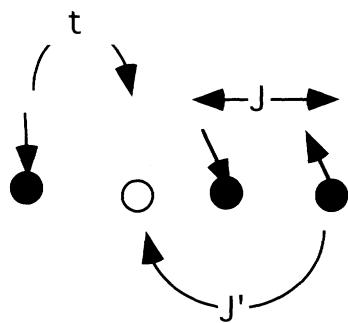
\includegraphics[width=0.6\textwidth]{fig3_1.jpg}
\caption{t--J 模型中空穴与自旋的相互作用。}
\label{fig:3.1}
\end{figure}

离开 t--J 模型之前，我们把它再写一遍——这次是正规排序形式：

\begin{equation*}
\mathcal {H} ^ {\mathrm{t-J}} = P _ {s} \left[ \mathcal {T} - \frac {1}{U} \sum_ {ijk} t _ {ij} t _ {jk} \left( c _ {i \uparrow} ^ {\dagger} c _ {j \downarrow} ^ {\dagger} - c _ {i \downarrow} ^ {\dagger} c _ {j \uparrow} ^ {\dagger} \right) \left( c _ {j \downarrow} c _ {k \uparrow} - c _ {j \uparrow} c _ {k \downarrow} \right) \right] P _ {s}.
\tag{3.33}
\end{equation*}

在第 19 章中，我们将用自旋--空穴相干态处理 t--J 模型。在定义其大自旋推广之后，我们将导出稀疏空穴密度的半经典理论。

\section{负 $U$ 模型}

负 $U$ Hubbard 模型描述电子之间的局域吸引相互作用。与排斥情形一样，应当把这个模型视为一个参数已重整化的有效模型，适用于低频与低温。当电子使某个集体自由度极化时，它们可以通过共享这一极化获得负的配对结合能 $-U$。

产生电子间吸引的极化机制已有多种提案，列举几个：晶格形变（声子）、集体电荷振荡（等离激元）、自旋涨落（顺磁振子）。在负 $U$ 相互作用中，极化机制的时间尺度（如声子的 Debye 频率）相对跳跃时间被视为瞬时的\footnote{这与超导电性的 Migdal--Eliashberg 近似正好处在相反的区间，参见 Schrieffer 的书。}。

我们讨论如下形式的哈密顿量：

\begin{align*}
\mathcal {H} ^ {-U} & = - \sum_ {ijs} t _ {ij} \, c _ {is} ^ {\dagger} c _ {js} - \frac {U}{2} \sum_ {i} ( n _ {i} - 1 ) ^ {2}\\
& \quad + \frac {1}{2} \sum_ {ij} V _ {ij} ( n _ {i} - 1 ) ( n _ {j} - 1 ) - \mu \sum_ {i} n _ {i}.
\tag{3.34}
\end{align*}

负 $U$ 项有利于同一格点上上、下自旋的局域配对。但跳跃项 $t_{ij}c_{is}^{\dagger}c_{js}$ 与这一倾向竞争，因为它使电子离域化、拆散配对。格点间相互作用 $V_{ij}$ 排斥不同格点上的电子，在半满附近对选定基态尤为重要。

第一步，只对下自旋电子作粒子--空穴变换，把 (3.34) 变成正 $U$ 模型：

\begin{align*}
c _ {i \uparrow} & \rightarrow \tilde {c} _ {i \uparrow} ,\\
c _ {i \downarrow} & \rightarrow \tilde {c} _ {i \downarrow} ^ {\dagger}.
\tag{3.35}
\end{align*}

这是一个正则的 Bogoliubov 变换（见 A.1 节），“赝电子”$\tilde{c}$ 满足 Fermi 反对易关系。利用 $\tilde{n}_{is}^{2} = \tilde{n}_{is}$，(3.34) 立即变成正 $U$ 哈密顿量

\begin{align*}
\mathcal {H} ^ {-U} \to \tilde {\mathcal {H}} ^ {+U} & = - \sum_ {ij} t _ {ij} \left( \tilde {c} _ {i \uparrow} ^ {\dagger} \tilde {c} _ {j \uparrow} - \tilde {c} _ {i \downarrow} ^ {\dagger} \tilde {c} _ {j \downarrow} \right) + \frac {U}{2} \sum_ {i} ( \tilde {n} _ {i} - 1 ) ^ {2}\\
& \quad + \frac {1}{2} \sum_ {ij} J _ {ij} ^ {a} \tilde {S} _ {i} ^ {z} \tilde {S} _ {j} ^ {z} - h \sum_ {i} \tilde {S} _ {i} ^ {z} - \mathcal {N} \Delta E,
\tag{3.36}
\end{align*}

其中 Ising 各向异性为

\begin{equation*}
J _ {ij} ^ {a} = 4 V _ {ij},
\tag{3.37}
\end{equation*}

磁场为

\begin{equation*}
h = 2 \mu ,
\tag{3.38}
\end{equation*}

能量平移为

\begin{equation*}
\Delta E = \mu + \frac {1}{2} U.
\tag{3.39}
\end{equation*}

现在对跳跃参数 $t_{ij}$ 定义二分格子（bipartite lattice）。

\medskip
\noindent\textbf{定义 3.1}\quad 若一个格子可以分成两个不相交的子晶格 $A$ 与 $B$，使得 $t_{ij}$ 只连接 $i \in A$ 到 $j \in B$（或 $i \in B$ 到 $j \in A$），则称之为二分格子。
\medskip

二分格子的常见例子是正方格子与立方格子。非二分的例子有三角格子与面心立方（FCC）格子的键。

注意 (3.36) 中的相互作用项为正，而跳跃矩阵元带有依赖自旋的正负号。这对非二分格子有重要的物理意义：在那里这些符号无法通过简单的规范变换消去。

\subsection{赝自旋模型与超导电性}

变换 (3.35) 把负 $U$ 模型的电荷算符映射为正 $U$ 模型的赝自旋算符。特别地，局域电荷涨落映射为 $z$ 方向的赝自旋：

\begin{equation*}
\frac {1}{2} ( n _ {i} - 1 ) \Leftrightarrow \tilde {S} _ {i} ^ {z}.
\tag{3.40}
\end{equation*}

于是，负 $U$ 模型偏离半满对应于正 $U$ 模型中 $S^{z}$ 方向的均匀磁化；类似地，负 $U$ 模型中的电荷密度波对应于正 $U$ 模型中的 $z$ 自旋密度波。

赝自旋分量 $\tilde{S}^x$、$\tilde{S}^y$ 对应于配对算符：

\begin{align*}
\frac {1}{2} \left( c _ {i \uparrow} ^ {\dagger} c _ {i \downarrow} ^ {\dagger} + c _ {i \downarrow} c _ {i \uparrow} \right) & \Leftrightarrow \tilde {S} _ {i} ^ {x},\\
\frac {1}{2i} \left( c _ {i \uparrow} ^ {\dagger} c _ {i \downarrow} ^ {\dagger} - c _ {i \downarrow} c _ {i \uparrow} \right) & \Leftrightarrow \tilde {S} _ {i} ^ {y}.
\tag{3.41}
\end{align*}

于是，赝自旋在 $x$--$y$ 平面内的有序代表负 $U$ 模型中的超导电性：

\begin{equation*}
\Psi ( \mathbf {x} _ {i} ) = \Delta ( \mathbf {x} _ {i} ) \, e ^ {i \phi ( \mathbf {x} _ {i} )} \Leftrightarrow \langle \tilde {S} _ {i} ^ {+} \rangle .
\tag{3.42}
\end{equation*}

有序矩的大小是 BCS 序参量 $\Delta$，其在 $x$--$y$ 平面内的角度是超导相位 $\phi$（参见 Schrieffer 的书，见文献注释）。$\Psi$ 以电荷 $2e$ 与外电磁规范场耦合。对缓变 $\Psi(\mathbf{x})$ 的自由能展开给出 Ginzburg--Landau 自由能泛函，后者产生了超导电性的大部分宏观唯象学（如磁通量子化、持续电流等）。

注意 $H^{+U}$ 的化学势为零。现在证明一个重要定理。

\medskip
\noindent\textbf{定理 3.2}\quad 对 $\mathcal{H}^{-U}$ 的任何电子填充，正 $U$ 模型 $\tilde{\mathcal{H}}^{+U}$ 恰好处于半满。
\medskip

证明很简单。考虑变换

\begin{equation*}
\tilde {c} _ {is} \rightarrow \tilde {c} _ {i,-s} ^ {\dagger} \, , \quad s = \uparrow , \downarrow .
\tag{3.43}
\end{equation*}

容易验证 $\tilde{H}^{+U}$ 在此变换下不变：

\begin{equation*}
\tilde {\mathcal {H}} ^ {+U} [ \tilde {c} ' ] = \tilde {\mathcal {H}} ^ {+U} [ \tilde {c} ],
\tag{3.44}
\end{equation*}

而

\begin{equation*}
\tilde {n} _ {i} \rightarrow 2 - \tilde {n} _ {i} '.
\tag{3.45}
\end{equation*}

电子数由热力学平均给出：

\begin{equation*}
\langle \tilde {n} _ {i} \rangle = \frac {1}{Z} \mathrm{Tr}_{\tilde{c}} \left( e ^ {- \beta \tilde {\mathcal {H}} ^ {+U} [ \tilde {c} ]} \tilde {n} _ {i} \right) = \frac {1}{Z} \mathrm{Tr}_{\tilde{c}'} \left[ e ^ {- \beta \tilde {\mathcal {H}} ^ {+U} [ \tilde {c} ' ]} ( 2 - \tilde {n} _ {i} ' ) \right],
\tag{3.46}
\end{equation*}

由于 (3.43) 是正则变换，迹在变换下不变，故\footnote{这里通过对有限格子定义平均，回避了局域自发对称性破缺（即相分离）的微妙之处。}

\begin{equation*}
\mathcal {N} ^ {- 1} \left\langle \sum_ {i} \tilde {n} _ {i} \right\rangle = \mathcal {N} ^ {- 1} \left\langle \sum_ {i} ( 2 - \tilde {n} _ {i} ) \right\rangle = 1,
\tag{3.47}
\end{equation*}

证毕。

定理 3.2 很重要，因为大 $U$ 时正 $U$ Hubbard 模型的半满极限可以约化为纯自旋问题。循 3.2 节的推导，有效赝自旋哈密顿量为

\begin{align*}
\tilde {\mathcal {H}} ^ {+U} & \rightarrow \tilde {\mathcal {H}} ^ {-x-xz} + \mathcal {O} ( t ^ {2} / U ),\\
\tilde {\mathcal {H}} ^ {-x-xz} & = \frac {1}{2} \sum_ {\langle ij \rangle} \left[ ( J _ {ij} + J _ {ij} ^ {a} ) \tilde {S} _ {i} ^ {z} \tilde {S} _ {j} ^ {z} - J _ {ij} ( \tilde {S} _ {i} ^ {x} \tilde {S} _ {j} ^ {x} + \tilde {S} _ {i} ^ {y} \tilde {S} _ {j} ^ {y} ) \right] - h \sum_ {i} \tilde {S} _ {i} ^ {z},
\tag{3.48}
\end{align*}

其中超交换耦合仍是 $J_{ij} = 4t_{ij}^{2}/U$。常数能量平移已略去。$\tilde{H}^{-x-xz}$ 是各向异性 Heisenberg 模型：$x, y$ 自旋分量为铁磁耦合，$z$ 分量为反铁磁耦合。

哈密顿量 (3.48) 是一个量子磁性模型，可以用本书描述的许多方法处理。在第 11 章我们将学到，半经典近似适用于二维和三维的破缺对称相。经典基态由极小化经典哈密顿量 $\tilde{\mathcal{H}}^{-x-xz}[\tilde{\mathbf{S}}]$ 得到，其中 $\tilde{\mathbf{S}}$ 是大小为 $S$ 的矢量。对非二分格子（如三角或面心立方格子）上的近邻模型，$z$ 自旋耦合是受挫的（见图~\ref{fig:3.2} 左三角形的底边键）；与此同时，铁磁的 $x$--$y$ 耦合可以完全满足（见右三角形）。结果，经典近似给出 $x$--$y$ 赝自旋有序，即低温超导电性。我们将看到，大的量子与热涨落可以破坏磁序，在低维尤其如此；超导电性同样受制于这些失序机制。

\begin{figure}[H]
\centering
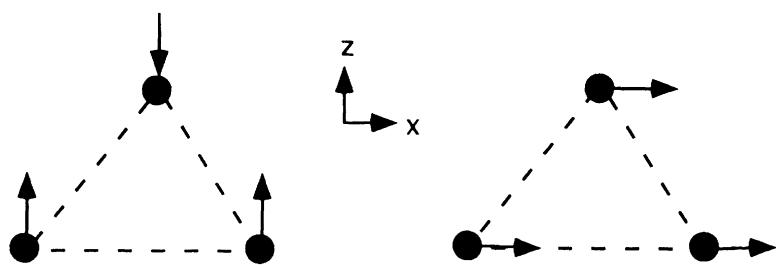
\includegraphics[width=0.52\textwidth]{fig3_2.jpg}
\caption{赝自旋哈密顿量 $H^{-x-xz}$：受挫的 $z$ 自旋耦合（左三角形）与满足的 $x$--$y$ 耦合（右三角形）。}
\label{fig:3.2}
\end{figure}

对二分格子\footnote{这里使用定义 3.1，把 $t_{ij}$ 换成 $J_{ij}$。}，把子晶格 B 上所有自旋绕 $z$ 轴旋转 $\pi$，即可把 $\tilde{\mathcal{H}}^{-x-xz}$ 化为 Ising--Heisenberg 形式

\begin{equation*}
\tilde {\mathcal {H}} ^ {-x-xz} \rightarrow \tilde {\mathcal {H}} ^ {xxz} = \frac {1}{2} \sum_ {ij} \left( J _ {ij} \, \tilde {\mathbf {S}} _ {i} \cdot \tilde {\mathbf {S}} _ {j} + J _ {ij} ^ {a} \tilde {S} _ {i} ^ {z} \tilde {S} _ {j} ^ {z} \right) - h \sum_ {i} \tilde {S} _ {i} ^ {z}.
\tag{3.49}
\end{equation*}

$\tilde{H}^{xxz}[\tilde{S}]$ 的基态是反铁磁的：赝自旋在两个子晶格上指向相反方向。$J^{a}=0$、$h=0$ 时，(3.49) 的经典基态具有 $O(3)$ 简并，序参量可指向球面上任何方向。$h>0$ 时简并降至 $O(2)$，因为 $z$ 方向的均匀磁场偏爱自旋大体躺在 $x$--$y$ 平面内——自旋的倾倒带来线性于 $h$ 的能量增益；见图~\ref{fig:3.3}。

然而，当 Ising 各向异性有限（$J^{a} > 0$）时，即使磁场很小，自旋也倾向于沿 $z$ 方向排列。磁场与 Ising 各向异性的竞争决定有序矩的方向。Ising 有序与 $x$--$y$ 有序之间的转变在磁场 $h$ 下可以是一阶或二阶。这一转变在真实磁性体系中无论理论上还是实验上都已被充分研究，并被应用于铋酸盐超导体的超导理论和氦-4 的超流理论（见文献注释）。在经典平均场近似下，转变的级次取决于次近邻相互作用的符号。一阶转变称为自旋翻转（spin-flop），在磁场--温度相图上意味着一个双临界点。二阶转变则意味着一个中间混合相，序参量同时具有 $z$ 与 $x$--$y$ 分量（即电荷密度波与超导电性共存）。对氦而言，混合相称为“超固体”，迄今尚未在实验上发现。

\begin{figure}[H]
\centering
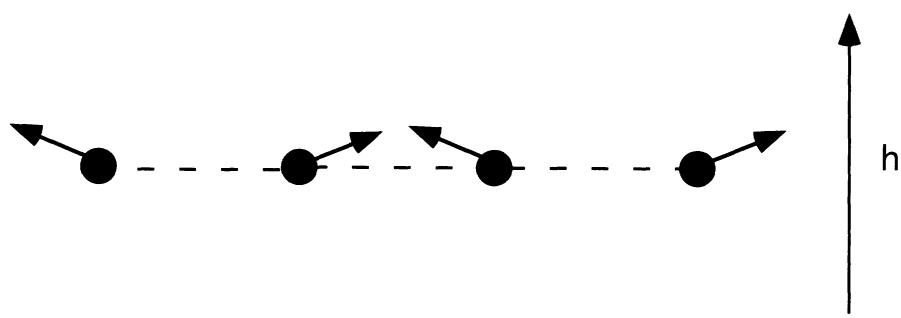
\includegraphics[width=0.52\textwidth]{fig3_3.jpg}
\caption{均匀磁场中反铁磁体的自旋翻转态。}
\label{fig:3.3}
\end{figure}

有效哈密顿量 (3.48) 是在大 $|U| \gg t$ 下导出的，它描述束缚在约一格常量尺度上的紧致电子对。弱耦合 $|U| < t$ 时，更好做法是对相互作用强度用微扰论，或用 4.1 节描述的那类变分磁态。当电荷激发存在能隙时，弱耦合与强耦合定性相似。弱耦合下，若费米面有大片平行部分（嵌套），也会出现这样的能隙。此时赝自旋模型 $\tilde{H}^{-x-xz}$ 可作为有效模型使用，在 Cooper 对的尺度上粗粒化——也就是说，“格点常量”应换成超导关联长度。

\begin{exercises}

\item 证明导出 Heisenberg 哈密顿量 (3.30) 时用到的恒等式：

\begin{equation*}
P _ {s} \left[ \sum_ {ss'} c _ {is} ^ {\dagger} c _ {js} \, n _ {j \uparrow} n _ {j \downarrow} \, c _ {js'} ^ {\dagger} c _ {is'} \right] P _ {s} = - 2 P _ {s} \left[ \mathbf {S} _ {i} \cdot \mathbf {S} _ {j} - \frac {n _ {i} n _ {j}}{4} \right] P _ {s}.
\tag{3.50}
\end{equation*}

\item 通过重排费米子算符，证明 (3.33) 的 t--J 模型等于 (3.25)。

\item 求两格点 Hubbard 模型 (3.14)（$i = 1,2$）在 $N_e = 1, 2, 3$ 个电子时的全部本征能量与本征态。$N_e = 2$ 时单态--三重态劈裂是多少？这就是有效自旋超交换常数。

提示：在每个填充 $N_{e}$ 下，把哈密顿量作为相关 Fock 态上的矩阵对角化。对 $4 \times 4$ 格子，这个矩阵有多大？

\item 证明 Hubbard 哈密顿量 (3.14) 与总自旋 $S_{tot} = \sum_{i} S_{i}$ 对易，从而是转动不变的。在一维 $N$ 格点的环上，其本征态由哪些量子数分类？

\end{exercises}

\begin{chapbib}
\item 关于 Hubbard 模型的一本新近综合参考书（收录该领域许多重要论文）：
  \textit{The Hubbard Model}, edited by A. Montorosi (World Scientific, 1992)。
\item 一维精确解参看：
  \textit{The Many Body Problem --- An Encyclopedia of Exactly Solved Models in One Dimension}, edited by D. C. Mattis (World Scientific, 1993)。
\item 一维的场论与重整化群技术参看：
  V. J. Emery, \textit{The Many Body Problem in One Dimension}, in ``Correlated Electron Systems'', edited by V. J. Emery (World Scientific, 1993)；
  H. J. Schultz, \textit{Interacting Fermions in One Dimension}, 同卷。
\item 超导电性的基本教科书：
  J. R. Schrieffer, \textit{Theory of Superconductivity} (Benjamin-Cummings, 1983)。
\item 负 $U$ 模型被提出用于铋酸盐超导体：
  T. M. Rice and L. Sneddon, Phys. Rev. Lett. \textbf{47}, 689 (1981)；
  A. S. Alexandrov, J. Ranninger, and S. Robaszkiewicz, Phys. Rev. B \textbf{33}, 4526 (1986)；
  A. Aharony and A. Auerbach, Phys. Rev. Lett. \textbf{70}, 1874 (1993)。
\item 磁学文献中对自旋翻转转变的分析见：
  \textit{Elements of Theoretical Magnetism}, edited by S. Krupicka and J. Sternberk (Iliffe), 7.4 节；
  M. E. Fisher and D. R. Nelson, Phys. Rev. Lett. \textbf{32}, 1350 (1974)。
\item 在超流氦的语境下，赝自旋模型与超固体的可能性有很长的历史：
  T. Matsubara and H. Matsuda, Prog. Theor. Phys. \textbf{16}, 569 (1956)；
  H. Matsuda and T. Tsuneto, Suppl. Prog. Theor. Phys. \textbf{46}, 411 (1970)；
  K. S. Liu and M. E. Fisher, J. Low Temp. Phys. \textbf{10}, 655 (1973)；\textbf{17}, 129 (1957)。
\item 关于包含 (3.10) 之 $J^F$ 项的 Hubbard 模型推广的讨论，见
  J. E. Hirsch, Phys. Rev. B \textbf{40}, 9061 (1989)。
\end{chapbib}


% 第二部分 波函数与关联
\part{波函数与关联}
\vspace{2em}
\begin{center}
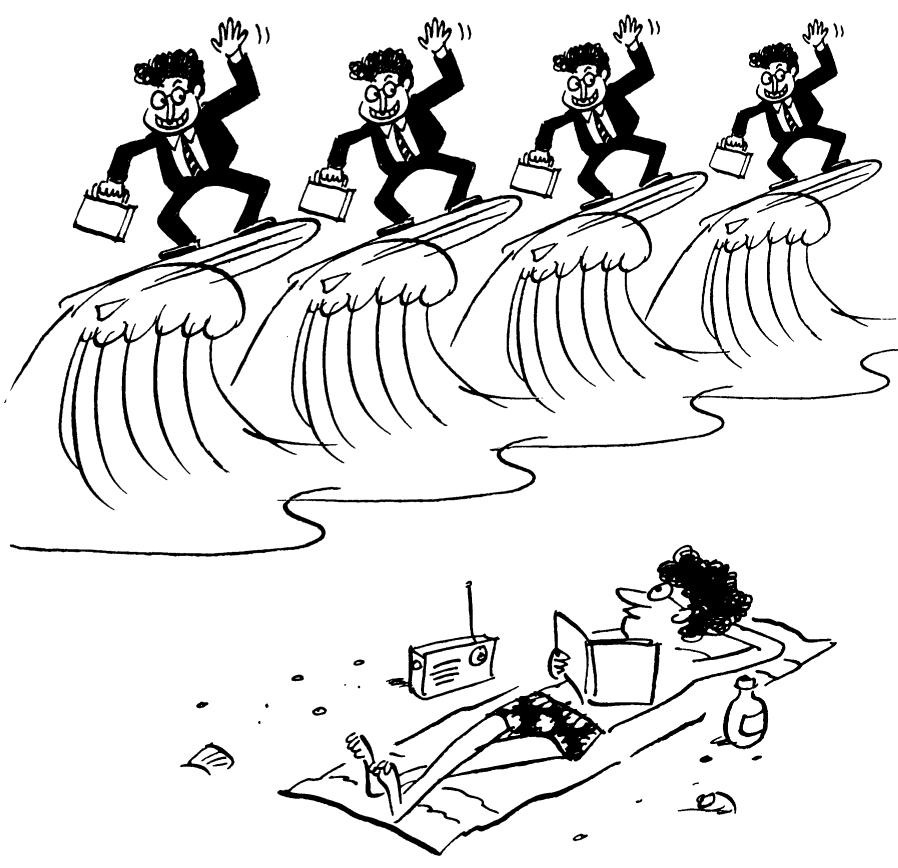
\includegraphics[width=0.5\textwidth]{deco_part2.jpg}

{\kaishu 插图：Dick Codor}
\end{center}

% 第4章 Hubbard 模型的基态
\chapter{Hubbard 模型的基态}

理解一个量子哈密顿量的第一步是寻找它的基态。在没有精确解的情况下，恰当地选取一族变分态 $\Psi^{\gamma}$（$\gamma$ 为变分参数）可能颇有收获。变分定理说

\begin{equation*}
\frac {\langle \Psi^ {\gamma} | \mathcal {H} | \Psi^ {\gamma} \rangle}{\langle \Psi^ {\gamma} | \Psi^ {\gamma} \rangle} = E ^ {\gamma} \geq E _ {0},
\tag{4.1}
\end{equation*}

其中 $E_{0}$ 是精确基态能量。对越来越大的变分态族极小化 (4.1) 左端，可以系统地改进基态能量与波函数。变分途径概念上直截了当，并且避开了困扰微扰论与渐近展开的那些数学上微妙的收敛问题。

另一方面，必须记住：对基态\emph{有序}而言，变分途径可能严重误导。能量主要对短程关联敏感，因此在受限的试探态族内，能量最低的态可能具有错误的长程关联。

本章重点讨论 Hubbard 模型的磁关联。4.1 节用自旋密度波 Fock 态演示变分途径，这给出零温 Hartree--Fock 理论的一个变分推导。

第二节给出（不加证明）关于有限格子上基态总自旋的若干定理。随后各章讨论半满下的磁行为，即 Heisenberg 模型。对偏离半满的 Hubbard 模型感兴趣的读者会发现第 19 章很有用：那里用 t--J 模型的大自旋推广，对二维掺杂反铁磁体（与铜氧化物超导体相关）作了半经典处理。

\section{变分磁态}

考虑如下形式的 Hubbard 模型：

\begin{equation*}
\mathcal {H} = \sum_ {\mathbf {k},\, s = \uparrow \downarrow} \epsilon_ {\mathbf {k}} \, c _ {\mathbf {k} s} ^ {\dagger} c _ {\mathbf {k} s} + U \sum_ {i} n _ {i \uparrow} n _ {i \downarrow}.
\tag{4.2}
\end{equation*}

最简单的变分态是 Fock 态（见 A.1 节）：

\begin{equation*}
| \{n _ {\alpha} ^ {\gamma} \} \rangle ,
\tag{4.3}
\end{equation*}

其中 $\alpha$ 标记单粒子态 $\{\phi_{\alpha}^{\gamma}\}$，$\gamma$ 是一组变分参数。(4.3) 中四个 Fermi 算符的期望值因子化\footnote{这里不包括反常期望值（如 $\langle c^{\dagger}c^{\dagger}\rangle$）的可能性，它们存在于 BCS 态中。}为

\begin{equation*}
\langle c _ {1} ^ {\dagger} c _ {3} ^ {\dagger} c _ {4} c _ {2} \rangle = \langle c _ {1} ^ {\dagger} c _ {2} \rangle \langle c _ {3} ^ {\dagger} c _ {4} \rangle - \langle c _ {1} ^ {\dagger} c _ {4} \rangle \langle c _ {3} ^ {\dagger} c _ {2} \rangle .
\tag{4.4}
\end{equation*}

描述磁有序的 Fock 态称为\textbf{自旋密度波态}。把原电子算符 $c_{\mathbf{k}s}$ 通过正则变换变成磁准粒子 $\alpha_{\mathbf{k}\pm}$ 即可构造这类态：

\begin{align*}
\alpha_ {\mathbf {k} +} ^ {\dagger} & = \cos \theta_ {\mathbf {k}} \, c _ {\mathbf {k} \uparrow} ^ {\dagger} + \sin \theta_ {\mathbf {k}} \, c _ {\mathbf {k} + \mathbf {q}, \downarrow} ^ {\dagger},\\
\alpha_ {\mathbf {k} -} ^ {\dagger} & = - \sin \theta_ {\mathbf {k}} \, c _ {\mathbf {k} \uparrow} ^ {\dagger} + \cos \theta_ {\mathbf {k}} \, c _ {\mathbf {k} + \mathbf {q}, \downarrow} ^ {\dagger}.
\tag{4.5}
\end{align*}

变分自旋密度波态由如下族给出：

\begin{equation*}
| \Psi^ {\mathbf {q}, \theta_ {\mathbf {k}}, \Sigma_ {F}} \rangle = \prod_ {\sigma = \pm ,\; \mathbf {k} \in \Sigma_ {F} ^ {\pm}} \alpha_ {\mathbf {k} \sigma} ^ {\dagger} | 0 \rangle .
\tag{4.6}
\end{equation*}

$\Psi$ 的变分参数是序波矢 $\mathbf{q}$、角度 $\theta_{\mathbf{k}}$，以及占据数 $n_{\mathbf{k}}^{\pm}=1,0$。后者定义了围住 $n\mathcal{N}$ 个被占态的两个费米面 $\Sigma_{F}^{\pm}$：

\begin{align*}
n & = \frac {1}{\mathcal {N}} \sum_ {\sigma , \mathbf {k}} n _ {\mathbf {k}} ^ {\sigma},\\
n _ {\mathbf {k}} ^ {\sigma} & = \left\{ \begin{array}{ll} 1 & \mathbf {k} \in \Sigma_ {F} ^ {\sigma} \\ 0 & \mathbf {k} \notin \Sigma_ {F} ^ {\sigma} \end{array} \right. .
\tag{4.7}
\end{align*}

变分参数由极小化 $\Psi$ 的能量确定。$\Psi$ 可以支撑波矢 $\mathbf{q}$ 处 $x$--$y$ 方向的非零磁化，也可支撑 $z$ 方向的均匀磁化。计算如下自旋算符的期望值即可看出：

\begin{figure}[H]
\centering
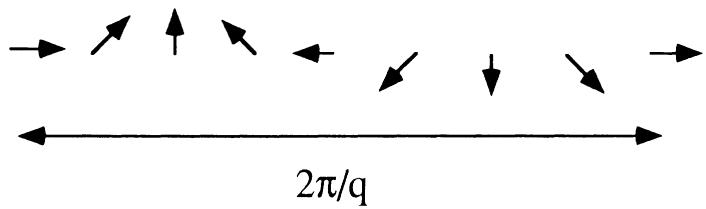
\includegraphics[width=0.5\textwidth]{fig4_1.jpg}
\caption{波矢 $\mathbf{q}$ 的螺旋自旋序。}
\label{fig:4.1}
\end{figure}

\begin{align*}
\langle S _ {i} ^ {+} \rangle & = \frac {1}{\mathcal {N}} \sum_ {\mathbf {q} '} e ^ {- i \mathbf {q} ' \mathbf {x} _ {i}} \sum_ {\mathbf {k}} \langle c _ {\mathbf {k} \uparrow} ^ {\dagger} c _ {\mathbf {k} + \mathbf {q}', \downarrow} \rangle\\
& = \frac {1}{\mathcal {N}} \sum_ {\mathbf {q} '} e ^ {- i \mathbf {q} ' \mathbf {x} _ {i}} \sum_ {\mathbf {k}} \Big( \sin \theta_ {\mathbf {k} + \mathbf {q} - \mathbf {q} '} \cos \theta_ {\mathbf {k}} \, \langle \alpha_ {\mathbf {k} +} ^ {\dagger} \alpha_ {\mathbf {k} + \mathbf {q} - \mathbf {q}', +} \rangle\\
& \qquad\qquad - \sin \theta_ {\mathbf {k}} \cos \theta_ {\mathbf {k} + \mathbf {q} - \mathbf {q} '} \, \langle \alpha_ {\mathbf {k} -} ^ {\dagger} \alpha_ {\mathbf {k} + \mathbf {q} - \mathbf {q}', -} \rangle \Big)\\
& = m _ {\mathbf {q}} \, e ^ {- i \mathbf {q} \mathbf {x} _ {i}} ,\\
m _ {\mathbf {q}} & = \frac {1}{2 \mathcal {N}} \sum_ {\mathbf {k}} \sin ( 2 \theta_ {\mathbf {k}} ) \left( n _ {\mathbf {k}} ^ {+} - n _ {\mathbf {k}} ^ {-} \right).
\tag{4.8}
\end{align*}

动量空间中的自旋算符满足

\begin{equation*}
\langle S ^ {+} ( \mathbf {q} ) \rangle = \langle S ^ {-} ( - \mathbf {q} ) \rangle ^ {*}.
\tag{4.9}
\end{equation*}

$m_{\mathbf{q}} \neq 0$ 描述 $x$--$y$ 平面内的螺旋自旋，自旋角度为 $\mathbf{q} \cdot \mathbf{x}_i$，如图~\ref{fig:4.1} 所示。

$z$ 方向的磁化由序参量

\begin{align*}
\langle S _ {i} ^ {z} \rangle & = \frac {1}{2} \sum_ {\mathbf {q} '} e ^ {- i \mathbf {q} ' \cdot \mathbf {x} _ {i}} \sum_ {\mathbf {k}} \langle c _ {\mathbf {k} \uparrow} ^ {\dagger} c _ {\mathbf {k} + \mathbf {q}', \uparrow} - c _ {\mathbf {k} \downarrow} ^ {\dagger} c _ {\mathbf {k} + \mathbf {q}', \downarrow} \rangle\\
& = \mathcal {N} m _ {z} ,\\
m _ {z} & = \frac {1}{2 \mathcal {N}} \sum_ {\mathbf {k}} \cos ( 2 \theta_ {\mathbf {k}} ) \left( n _ {\mathbf {k}} ^ {+} - n _ {\mathbf {k}} ^ {-} \right)
\tag{4.10}
\end{align*}

描述。利用 (4.4)，Hubbard 相互作用的期望值为

\begin{align*}
\Big\langle U \sum_ {i} n _ {i \uparrow} n _ {i \downarrow} \Big\rangle & = U \sum_ {i} \langle n _ {i \uparrow} \rangle \langle n _ {i \downarrow} \rangle - U \sum_ {i} \langle S _ {i} ^ {+} \rangle \langle S _ {i} ^ {-} \rangle\\
& = \mathcal {N} U \frac {n ^ {2}}{4} - \mathcal {N} U m _ {z} ^ {2} - \mathcal {N} U m _ {\mathbf {q}} ^ {2}.
\tag{4.11}
\end{align*}

动能项的期望值为

\begin{align*}
T & \equiv \Big\langle \sum_ {\mathbf {k}, s} \epsilon_ {\mathbf {k}} \, c _ {\mathbf {k} s} ^ {\dagger} c _ {\mathbf {k} s} \Big\rangle\\
& = \sum_ {\pm \mathbf {k}} \left[ \frac {\epsilon_ {\mathbf {k}} + \epsilon_ {\mathbf {k} + \mathbf {q}}}{2} \pm \left( \frac {\epsilon_ {\mathbf {k}} - \epsilon_ {\mathbf {k} + \mathbf {q}}}{2} \right) \cos ( 2 \theta_ {\mathbf {k}} ) \right] n _ {\mathbf {k}} ^ {\pm}.
\tag{4.12}
\end{align*}

从 $T$ 中减去 $-2(\mathcal{N}Um_{z}^{2}-\mathcal{N}Um_{\mathbf{q}}^{2})$ 并把它加到能量上，得到基态能量的变分表达式：

\begin{equation*}
E [ \mathbf {q}, \theta_ {\mathbf {k}}, \Sigma^ {\pm} ] = E ^ {0} + \mathcal {N} U m _ {z} ^ {2} + \mathcal {N} U m _ {\mathbf {q}} ^ {2} + \mathcal {N} U n ^ {2} / 4,
\tag{4.13}
\end{equation*}

其中

\begin{equation*}
E ^ {0} = \sum_ {\pm \mathbf {k}} E _ {\mathbf {k}} ^ {\pm} \, n _ {\mathbf {k}} ^ {\pm}.
\tag{4.14}
\end{equation*}

$E_{\mathbf{k}}^{\pm}$ 是“磁带能量”，定义为\footnote{这里 $E_{\mathbf{k}}$ 是基态的变分参数，并非模型的真正激发。}

\begin{equation*}
E _ {\mathbf {k}} ^ {\pm} = \frac {\epsilon_ {\mathbf {k}} + \epsilon_ {\mathbf {k} + \mathbf {q}}}{2} \pm \left[ \left( \frac {\epsilon_ {\mathbf {k}} - \epsilon_ {\mathbf {k} + \mathbf {q}}}{2} - m _ {z} \right) \cos ( 2 \theta_ {\mathbf {k}} ) - U m _ {\mathbf {q}} \sin ( 2 \theta_ {\mathbf {k}} ) \right].
\tag{4.15}
\end{equation*}

容易验证，对 $m_{q}$ 与 $m_{z}$ 极小化 (4.14) 分别重新给出 (4.8) 与 (4.10)。因此可以把 $m_{z}$ 和 $m_{q}$ 当作自由变分参数，它们与 $\cos(2\theta_{k})$ 无关。现在必须极小化泛函 $E[m_{q}, m_{z}, q, \theta_{k}, \Sigma_{f}^{\pm}]$。由 (4.14) 显然可见，最优的 $\Sigma_{F}^{\pm}$ 是围住最低磁带能量的那些。

变分函数 $\cos(2\theta_{\mathbf{k}})$ 由

\begin{equation*}
\frac {\partial E}{\partial \cos ( 2 \theta_ {\mathbf {k}} )} = \left[ \frac {\epsilon_ {\mathbf {k}} - \epsilon_ {\mathbf {k} + \mathbf {q}}}{2} - U m _ {z} + U m _ {q} \cot ( 2 \theta_ {\mathbf {k}} ) \right] \left( n _ {\mathbf {k}} ^ {+} - n _ {\mathbf {k}} ^ {-} \right) = 0
\tag{4.16}
\end{equation*}

确定，从而给出 $\cos(2\theta_{\mathbf{k}})$ 对 $m_{z}$、$m_{q}$ 的显式依赖：

\begin{equation*}
\cos ( 2 \theta_ {\mathbf {k}} ) = \frac { \dfrac {\epsilon_ {\mathbf {k}} - \epsilon_ {\mathbf {k} + \mathbf {q}}}{2} - U m _ {z} }{ \sqrt { \left( \dfrac {\epsilon_ {\mathbf {k}} - \epsilon_ {\mathbf {k} + \mathbf {q}}}{2} - U m _ {z} \right) ^ {2} + ( U m _ {q} ) ^ {2} } }.
\tag{4.17}
\end{equation*}

把 (4.17) 代入 (4.15)，得到磁带

\begin{equation*}
E _ {\mathbf {k}} ^ {\pm} \left( m _ {z}, m _ {\mathbf {q}} \right) = \frac {\epsilon_ {\mathbf {k}} + \epsilon_ {\mathbf {k} + \mathbf {q}}}{2} \pm \sqrt { \left( \frac {\epsilon_ {\mathbf {k}} - \epsilon_ {\mathbf {k} + \mathbf {q}}}{2} + U m _ {z} \right) ^ {2} + U ^ {2} m _ {\mathbf {q}} ^ {2} }.
\tag{4.18}
\end{equation*}

两个序参量 $m_{z}$、$m_{q}$ 决定磁带、费米面以及 $E(m_{z}, m_{\mathbf{q}})$。对它们极小化给出耦合方程

\begin{align*}
\frac {d E}{d m _ {\mathbf {q}}} & = \frac {d E ^ {0}}{d m _ {\mathbf {q}}} - 2 \mathcal {N} U m _ {q} = 0,\\
\frac {d E}{d m _ {z}} & = \frac {d E ^ {0}}{d m _ {z}} - 2 \mathcal {N} U m _ {z} = 0.
\tag{4.19}
\end{align*}

方程 (4.19) 就是熟知的零温 Hartree--Fock 平均场方程。对任何无相互作用能带结构 $\epsilon_{k}$、填充 $n$ 与相互作用 $U$，它们可以（多数情况下数值地）求解。

由 (4.19) 可以得到顺磁态对形成磁态的不稳定性判据。设 $m_{q}=0$，把 (4.19) 按 $m_{z}$ 展开到线性阶，得到 $z$ 方向均匀磁化（$m_{z}\neq0$）出现的条件：

\begin{align*}
\frac {d E ^ {0}}{d m _ {z}} & = 4 U ^ {2} m _ {z} \, \chi \big| _ {m _ {z} = 0} + \mathcal {O} ( m _ {z} ^ {2} )\\
& = 2 m _ {z} U,
\tag{4.20}
\end{align*}

其中 $\chi$ 是无相互作用电子的均匀磁化率

\begin{equation*}
\chi ( 0 ) = \frac {1}{2} \sum_ {\mathbf {k}} \frac {d n ( \epsilon_ {\mathbf {k}} )}{d \epsilon_ {\mathbf {k}}} = \frac {1}{2} \rho_ {\uparrow} ( 0 ),
\tag{4.21}
\end{equation*}

$n(\epsilon) = (e^{\epsilon/T} + 1)^{-1}$ 是 Fermi 函数，$\rho_{\uparrow}(0)$ 是费米能处无相互作用的单自旋态密度。(4.21) 给出著名的铁磁失稳 Stoner 判据：

\begin{equation*}
2 U \chi ( 0 ) = 1.
\tag{4.22}
\end{equation*}

还必须检验向 $m_{q} \neq 0$ 自旋密度波态的不稳定性。设 $m_{z} = 0$，把 (4.19) 按 $m_{q}$ 展开到线性阶，得到存在 $m_{q} \neq 0$ 解的条件：

\begin{align*}
\frac {d E ^ {0}}{d m _ {\mathbf {q}}} & = 4 U ^ {2} m _ {\mathbf {q}} \, \chi ( \mathbf {q} ) \big| _ {m _ {\mathbf {q}} = 0} + \mathcal {O} ( m _ {\mathbf {q}} )\\
& = 2 m _ {\mathbf {q}} U,
\tag{4.23}
\end{align*}

其中 $\chi(\mathbf{q})$ 是波矢 $\mathbf{q}$ 处的磁化率：

\begin{equation*}
\chi ( \mathbf {q} ) = \frac {1}{2} \sum_ {\mathbf {k}} \frac {n \left( \epsilon_ {\mathbf {k} + \mathbf {q}} \right) - n \left( \epsilon_ {\mathbf {k}} \right)}{\epsilon_ {\mathbf {k}} - \epsilon_ {\mathbf {k} + \mathbf {q}}}.
\tag{4.24}
\end{equation*}

(4.23) 同样给出波矢 $\mathbf{q}$ 处自旋密度波失稳的 Stoner 判据：

\begin{equation*}
2 U \chi ( \mathbf {q} ) = 1.
\tag{4.25}
\end{equation*}

因此，当我们增大 $U$ 的数值时，使 $\chi(\mathbf{q})$ 最大的波矢就是磁失稳最先发生的序波矢。

由 (4.24) 可见，$\chi(0)$ 依赖于费米面态密度，而有限 $|q|$ 的 $\chi(\mathbf{q})$ 对费米面几何、特别是其嵌套（nesting）性质敏感。“嵌套”指费米面上存在相距波矢 $q_{nest}$ 的平行片段。这种效应在一维以及近半满的二维正方格子上最为显著。嵌套在 (4.24) 的和式中提供了大量的小能量分母 $|\epsilon_{k}-\epsilon_{k+q_{nest}}| \ll W$，从而增大 $\chi(\mathbf{q}_{nest})$。这一发散甚至可能对非常小的 $U/t$ 就产生磁性基态！

上面给出的磁态通常用于建模金属铁磁体（如铁）和自旋密度波体系（如铬）。在激发的 Hartree--Fock 平均场理论中，磁带结构中无能隙意味着存在低能载流激发，这类体系称为巡游磁体。

上述变分分析真正告诉我们的只是：最低的自旋密度波态能量低于其他试探 Fock 态（包括非磁的能带态）。然而，众所周知 Stoner 判据高估磁有序、低估自旋涨落引起的量子失序。有限温的 Hartree--Fock 方程甚至在一维、二维也给出长程磁序，这违反了第 6 章给出的 Mermin--Wagner 定理。因此我们只能得出结论：当 Stoner 判据被满足时，Hubbard 模型中至少存在短程磁有序。

这里我们只集中于磁性变分 Fock 态。此外还有描述电荷密度有序、超导电性或几种有序混合的其他变分 Fock 态\footnote{例如 3.3 节所示的超导电性与电荷密度波。}。类比 (4.5)，对电子实行别的正则变换即可得到它们。例如：混合不同动量的同自旋粒子可得电荷密度波；混合粒子与空穴则给出破缺规范对称的超导态。每一种可能都增添变分参数与平均场方程。求解角度与序参量只是把上面概述的计算作繁琐却直截了当的推广。

在离开变分态这个主题之前，还应当提到一族重要的非 Fock 态——Gutzwiller 态

\begin{equation*}
\Psi^ {g} = \prod_ {i} \left[ 1 - g \, n _ {i \uparrow} n _ {i \downarrow} \right] \Psi^ {\mathrm{Fock}},
\tag{4.26}
\end{equation*}

其中 $\Psi^{\mathrm{Fock}}$ 是任何变分 Fock 态，例如 (4.6)。$g$ 是一个附加参数，压低双占据格点态的相对权重；$g \rightarrow 1$ 完全消除双占据态。这一族中被研究得特别透彻的成员是一维 Gutzwiller 投影费米气体：

\begin{equation*}
\Psi^ {\mathrm{GPFG}} = \prod_ {i} \left( 1 - n _ {i \uparrow} n _ {i \downarrow} \right) \prod_ {| \mathbf {k} | \leq \pi / a} c _ {\mathbf {k} \uparrow} ^ {\dagger} c _ {\mathbf {k} \downarrow} ^ {\dagger} | 0 \rangle
\tag{4.27}
\end{equation*}

$\Psi^{\mathrm{GPFG}}$ 是纯自旋变分态。事实上，它是 $S = \frac{1}{2}$ 的 Haldane--Shastry Heisenberg 模型的精确基态，该模型的反铁磁耦合按 $1/r^{2}$ 随距离衰减。

Gutzwiller 态中能量与关联的计算远非平凡，因为它们不像 (4.4) 那样因子化。（对 $g$ 的）微扰展开涉及 $gn_{i\uparrow}n_{i\downarrow}$ 的大乘积。Vollhardt 与 Metzner 在一维解析地完成了这类计算。

\section{若干基态定理}

Hubbard 模型基态的总自旋与磁化满足若干一般性定理。这里我们不加详细证明地陈述其中一些。证明步骤本身富有启发性，鼓励读者直接从原始文献学习。以下所有定理都限于大小为 $\mathcal{N}$、电子数固定的有限格子。

\medskip
\noindent\textbf{Nagaoka 定理 4.1}\quad 无穷大 $U$ 模型在二分格子（见定义 3.1）上，

\begin{equation*}
\lim _ {U \to \infty} \mathcal {H} ^ {\mathrm{eff}} = - \sum_ {ijs} | t _ {ij} | \, P _ {s} c _ {is} ^ {\dagger} c _ {js} P _ {s},
\tag{4.28}
\end{equation*}

当 $N_{e} = \mathcal{N} - 1$ 时，其基态是完全极化的铁磁体，总自旋为

\begin{equation*}
S = \frac {1}{2} ( \mathcal {N} - 1 ).
\tag{4.29}
\end{equation*}
\medskip

一个（未归一化的）具有最大磁化的基态是

\begin{equation*}
\Psi^ {\uparrow} = \sum_ {i} ( - 1 ) ^ {i} \prod_ {i ' \neq i} c _ {i ' \uparrow} ^ {\dagger} | 0 \rangle .
\tag{4.30}
\end{equation*}

基态能量为 $-zt$，$z$ 是最近邻数目；总自旋由 (4.29) 给出。

\begin{figure}[H]
\centering
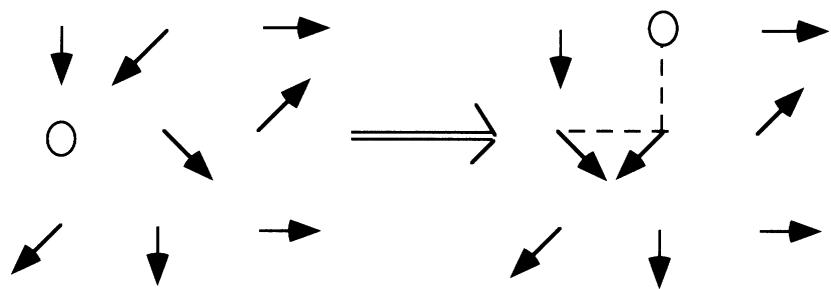
\includegraphics[width=0.5\textwidth]{fig4_2.jpg}
\caption{空穴在自旋背景中的两次跳跃。}
\label{fig:4.2}
\end{figure}

该定理的证明由 Yosuke Nagaoka 给出\footnote{见 Y. Nagaoka, Phys. Rev. \textbf{147}, 392 (1966)。}，此处不再重复。只需指出：证明通过遍及空穴的所有闭合跳跃路径求和，构造了几类格子的动力学单粒子 Green 函数。作为直接推论，通过粒子--空穴变换

\begin{equation*}
c _ {is} \rightarrow \eta_ {i} c _ {is} ^ {\dagger} \, , \quad \eta_ {i} = \left\{\begin{array}{ll}1 & i \in A\\- 1 & i \in B\end{array}\right.,
\tag{4.31}
\end{equation*}

它保持哈密顿量 (4.28) 不变并把 $N_e \to \mathcal{N} + 1$，定理 4.1 可以推广到高出半满一个电子的二分格子。

Nagaoka 铁磁性纯系动能起源：它来自空穴动能在完全排列一致的自旋组态中的极小化。论证如下：对任意自旋组态，跳跃的空穴会留下一串被平移的自旋，许多闭合路径并不能把自旋复原，因而被排除出动能；如图~\ref{fig:4.2} 所示。相反，铁磁自旋组态对任何闭合路径都回到原态，故其动能最小。更多内容见 Nagaoka 的原始论文与文献注释。

然而，这一结果既不能直接推广到有限 $U$，也不能推广到其他空穴密度。Nagaoka 哈密顿量 (4.28) 的激发谱有些病态。$N_{e} = \mathcal{N}$ 时，基态具有 $\mathcal{N}$ 个独立自旋 1/2 自由度带来的 $2^{\mathcal{N}}$ 重简并。这重简并极易被定理严格条件的任何偏离所破坏——有限温度、有限 $U$ 或不同填充都不例外。因此，在何种微扰下 Nagaoka 铁磁性得以存留，远非显然。这一定理的主要教益是：可动空穴倾向于在某个范围内或某个时间尺度上把背景自旋排齐。它暗示 t--J 模型中空穴周围可以形成局域的铁磁极化子（见第 19 章）。

我们还不加证明地提及 Elliot Lieb 的两个定理\footnote{E. Lieb, Phys. Rev. Lett. \textbf{62}, 1201 (1989)；勘误见同刊 \textbf{62}, 1927 (1989)。}。

\medskip
\noindent\textbf{Lieb 定理 4.2}\quad 考虑具有二分跳跃参数 $t_{ij}$（见定义 3.1）的正 $U$ Hubbard 模型

\begin{equation*}
\mathcal {H} = - \sum_ {sij} t _ {ij} \, c _ {is} ^ {\dagger} c _ {js} + \sum_ {i} | U _ {i} | \, n _ {i \uparrow} n _ {i \downarrow}.
\tag{4.32}
\end{equation*}

$N_{A}$、$N_{B}$ 分别是子晶格 A、B 上的格点数。设电子数 $N_{e} = N_{A} + N_{B}$（半满），则基态 $|\Psi_{0}\rangle$ 的总自旋满足

\begin{align*}
\mathbf {S} ^ {2} | \Psi_ {0} \rangle & = S ( S + 1 ) | \Psi_ {0} \rangle\\
S & = \frac {1}{2} \left| \mathcal {N} _ {A} - \mathcal {N} _ {B} \right| ,
\tag{4.33}
\end{align*}

且 $|\Psi_0\rangle$ 在平凡的 $(2S + 1)$ 重转动简并之外是唯一的。
\medskip

\medskip
\noindent\textbf{推论 4.3}\quad 因此，$N_{A} = N_{B}$ 的二分格子其基态是总单态（$S = 0$）且非简并。于是有限 $U$ 下（基态）不可能发生任何能级交叉。
\medskip

换言之，半满时的小 $U$ 与大 $U$ 基态是“绝热相连”的：随着 $U$ 增大，基态从自由电子气连续演化到 Heisenberg 反铁磁体的基态，正如 3.2 节所预期。第 5 章将描述 Heisenberg 模型的 Marshall 定理，它与 Lieb 定理 4.2 十分相似。两个定理都利用了哈密顿量的一个特性：在某个基底下其非对角矩阵元非正。这一性质使基态在该基底上正定，由此可证其唯一性与总自旋值。

3.3 节我们看到，任意填充的负 $U$ Hubbard 模型都与半满的正 $U$ 模型相关。因此定理 4.2 与下述定理密切相关。

\medskip
\noindent\textbf{Lieb 定理 4.4}\quad 考虑有限格子（$\mathcal{N} < \infty$）上的负 $U$ Hubbard 模型

\begin{equation*}
\mathcal {H} = - \sum_ {sij} t _ {ij} \, c _ {is} ^ {\dagger} c _ {js} - \sum_ {i} | U _ {i} | \, n _ {i \uparrow} n _ {i \downarrow},
\tag{4.34}
\end{equation*}

电子数为偶数，跳跃参数任意，$t_{ij} = t_{ji}$。则 (4.34) 的基态 $|\Psi_0\rangle$ 是总自旋 $\mathbf{S} = \sum_i\mathbf{S}_i$ 的单态：

\begin{equation*}
\mathbf {S} _ {\mathrm{tot}} ^ {2} | \Psi_ {0} \rangle = 0,
\tag{4.35}
\end{equation*}

而且它是唯一的。
\medskip

对 $|U/t| \gg 1$，此定理并不奇怪：基态预期是局域配对电子的体系。较小 $|U/t|$ 下基态的唯一性及其自旋则是定理 4.4 的非平凡结果。如 3.3 节所述，负 $U$ 哈密顿量描述电荷密度有序与超导电性的竞争。遗憾的是，基态的自旋无助于我们在热力学极限下分辨可能的对称性破缺；那必须靠其他手段确立（见第 6 章）。

\begin{exercises}

\item 求 (4.2) 的 $\mathcal{H}$ 在 Fermi 气体顺磁态

\begin{equation*}
\Psi^ {0} = \prod_ {s,\; \mathbf {k} \in \Sigma_ {F}} c _ {\mathbf {k} s} ^ {\dagger} | 0 \rangle ,
\tag{4.36}
\end{equation*}

中的期望值，其中 $\Sigma_{F}$ 是围住 $\frac{1}{2}\mathcal{N}n$ 个 $\mathbf{k}$ 值的费米面。

\item 把 (4.36) 的能量与完全极化铁磁态

\begin{equation*}
\Psi^ {\uparrow} = \prod_ {\mathbf {k} \in \Sigma_ {F} ^ {\uparrow}} c _ {\mathbf {k} \uparrow} ^ {\dagger} | 0 \rangle ,
\tag{4.37}
\end{equation*}

的能量比较，其中 $\Sigma_F^\uparrow$ 是围住 $N_e$ 个 $\mathbf{k}$ 态的单自旋费米面。$U/t$ 多大时铁磁态更优？把这个变分判据与 Stoner 判据 (4.22) 比较，孰强孰弱？

\item Stoner 条件 (4.22) 与铁磁耦合的 Hund 定则（见 2.1 节）之间有何联系与区别？

\end{exercises}

\begin{chapbib}
\item Hartree--Fock 近似与 Stoner 判据的 Green 函数推导见：
  S. Doniach and E. H. Sondheimer, \textit{Green's Functions for Solid State Physicists} (Benjamin/Cummings, 1974)。
\item 关于自旋密度波理论及实验的综合专著：
  T. Moriya, \textit{Spin Fluctuations in Itinerant Electron Magnetism} (Springer-Verlag, 1985)。
\item Hubbard 模型严格定理与未决问题的新近综述：
  E. Lieb, \textit{Proceedings of the conference Advances in Dynamical Systems and Quantum Physics}, Capri (World Scientific, 1993)。
\item Gutzwiller 变分态 (4.26) 提出于其经典论文：
  M. C. Gutzwiller, Phys. Rev. Lett. \textbf{10}, 159 (1963)。
\item Gutzwiller 态中关联的解析计算：
  W. Metzner and D. Vollhardt, Phys. Rev. B \textbf{37}, 7382 (1988)；
  F. Gebhard and D. Vollhardt, Phys. Rev. B \textbf{38}, 6911 (1988)。
\item Haldane--Shastry 模型引入于
  F. D. M. Haldane, Phys. Rev. Lett. \textbf{60}, 635 (1988)；
  B. S. Shastry, Phys. Rev. Lett. \textbf{60}, 639 (1988)，
  其中证明了基态正是 (4.27) 的 Gutzwiller 态 $\Psi^{\mathrm{GPFG}}$。
\end{chapbib}

% 第5章 Heisenberg 模型的基态
\chapter{Heisenberg 模型的基态}

3.2 节中，自旋 1/2 的反铁磁 Heisenberg 模型作为 Mott 绝缘体的有效哈密顿量出现。一般地说，Heisenberg 哈密顿量是量子磁学的基本模型，也是其他可以用量子自旋算符有效描述的现象的基本模型\footnote{例如 3.3 节所示的超导电性与电荷密度波。}。从其基态、激发与热力学相的研究中，可以学到极宽范围内的一批概念和技术。

大小为 $S$ 的 $\mathcal{N}$ 个自旋的格子，其哈密顿量为

\begin{align*}
\mathcal {H} & = \mathcal {H} ^ {zz} + \mathcal {H} ^ {xy} ,\\
\mathcal {H} ^ {zz} & = \frac {1}{2} \sum_ {ij} J _ {ij} S _ {i} ^ {z} S _ {j} ^ {z} ,\\
\mathcal {H} ^ {xy} & = \frac {1}{4} \sum_ {ij} J _ {ij} \left( S _ {i} ^ {+} S _ {j} ^ {-} + S _ {i} ^ {-} S _ {j} ^ {+} \right) ,\\
S _ {\mathrm{tot}} ^ {z} & = \sum_ {i} S _ {i} ^ {z} ,
\tag{5.1}
\end{align*}

其中 $J_{ij} = J_{ji}$ 具有格子平移对称性。$\mathcal{H}$ 与总自旋

\begin{equation*}
\mathbf {S} _ {\mathrm{tot}} = \sum_ {i} \mathbf {S} _ {i}
\tag{5.2}
\end{equation*}

的所有三个分量对易，因而是转动不变的。于是本征态可标记为

\begin{align*}
\Psi & = | S _ {\mathrm{tot}}, M, \ldots \rangle ,\\
M & = - S _ {\mathrm{tot}}, - S _ {\mathrm{tot}} + 1, \ldots , S _ {\mathrm{tot}} ,\\
S _ {\mathrm{tot}} & \leq \mathcal {N} S ,
\tag{5.3}
\end{align*}

$M$ 是总磁化 $S_{\mathrm{tot}}^{z}$ 的本征值，而

\begin{equation*}
\mathbf {S} _ {\mathrm{tot}} ^ {2} = S _ {\mathrm{tot}} \left( S _ {\mathrm{tot}} + 1 \right).
\tag{5.4}
\end{equation*}

若耦合 $J_{ij}$ 对 $i$、$j$ 的格子平移不变，则格子动量 $\mathbf{k}$ 也是好量子数。

本章集中于 Heisenberg 模型基态的两个方面。5.1 节证明关于总自旋与波函数符号的 Marshall 定理；5.2 节证明半奇整数自旋链在大 $\mathcal{N}$ 极限下的无能隙行为。

\section{反铁磁体}

一般而言，反铁磁基态远比铁磁基态复杂。下面的定理对二分反铁磁哈密顿量（见定义 3.1）的基态给出强约束。子晶格 A、B 上的交错磁化算符为

\begin{equation*}
S ^ {\mathrm{stagg}} = \sum_ {i \in A} S _ {i} ^ {z} - \sum_ {i \in B} S _ {i} ^ {z}.
\tag{5.5}
\end{equation*}

Ising 组态构成基底

\begin{equation*}
\Phi_ {\alpha} = \left| S, m _ {1} ^ {\alpha} \right\rangle_ {1} \left| S, m _ {2} ^ {\alpha} \right\rangle_ {2} \dots \left| S, m _ {\mathcal {N}} ^ {\alpha} \right\rangle_ {\mathcal {N}} ,
\tag{5.6}
\end{equation*}

其中 $|S, m_i \rangle_i$ 表示 $\mathbf{S}_i^2$、$S_i^z$ 的本征态，本征值分别为 $S(S + 1)$、$m_i$。使 $S^{\mathrm{stagg}}$ 极大的 Néel 态是 Ising 组态

\begin{equation*}
\Psi^ {\mathrm{N\acute{e}el}} = \prod_ {i} \left| S, \eta_ {i} S \right\rangle_ {i} \, , \quad \eta_ {i} = \left\{ \begin{array}{ll} 1 & i \in A \\ - 1 & i \in B \end{array} \right. .
\tag{5.7}
\end{equation*}

然而一般 $\Psi^{\mathrm{N\acute{e}el}}$ 并非 $\mathcal{H}$ 的本征态。“捣乱者”是 $H^{xy}$ 中的自旋翻转项 $S_{i}^{+}S_{j}^{-}$，它们把 $\Psi^{\mathrm{N\acute{e}el}}$ 与其他 Ising 组态联系起来。为了我们的目的，方便的做法是把子晶格 B 的自旋轴绕 $z$ 轴转动，即作幺正变换

\begin{align*}
i & \in B :\\
S _ {i} ^ {+} & \rightarrow - \tilde {S} _ {i} ^ {+} ,\\
S _ {i} ^ {-} & \rightarrow - \tilde {S} _ {i} ^ {-} ,\\
S _ {i} ^ {z} & \rightarrow + \tilde {S} _ {i} ^ {z} ,
\tag{5.8}
\end{align*}

它把 Ising 组态变为

\begin{equation*}
\left| S, m _ {i} \right\rangle_ {i} \to \left| S, \tilde {m} _ {i} \right\rangle_ {i} = \left\{ \begin{array}{ll} \left| S, m _ {i} \right\rangle_ {i} & i \in A \\ (- 1)^{(S + m _ {i})} \left| S, m _ {i} \right\rangle_ {i} & i \in B \end{array} \right. ,
\tag{5.9}
\end{equation*}

其中 $\tilde{m}_{i}$ 分别是子晶格 A 上 $S_{i}^{z}$ 与子晶格 B 上 $\tilde{S}_{i}^{z}$ 的本征值。把自己限制在某个 $M$ 子空间，把所有波函数展开为

\begin{equation*}
\Psi^ {M} = \sum_ {\alpha} f _ {\alpha} ^ {M} \tilde {\Phi} _ {\alpha} ^ {M},
\tag{5.10}
\end{equation*}

其中

\begin{equation*}
\tilde {\Phi} _ {\alpha} ^ {M} = \prod_{\sum_i \tilde m_i^\alpha = M} \left| S, \tilde {m} _ {i} ^ {\alpha} \right\rangle_ {i}.
\tag{5.11}
\end{equation*}

现在给出 Marshall 定理（经 Lieb 与 Mattis 推广，见文献注释）。

\medskip
\noindent\textbf{Marshall 定理 5.1}\quad 考虑哈密顿量 (5.1)，具有连接子晶格 $A$、$B$（二分）的反铁磁交换 $J_{ij} \geq 0$，且格子上任意两格点都可以经由中间格点的有限交换序列相连。则在任何允许的 $M$ 扇区中，最低能量态 $\Psi_0^M$ 可以取为在转动的 Ising 基 $\tilde{\Phi}_{\alpha}^{M}$ 中系数正定：

\begin{equation*}
\Psi_ {0} ^ {M} = \sum_ {\alpha} f _ {\alpha} ^ {M} \tilde {\Phi} _ {\alpha} ^ {M} \, , \quad f _ {\alpha} ^ {M} > 0, \; \forall \alpha .
\tag{5.12}
\end{equation*}
\medskip

因此，由 (5.8)，$\Psi_0^M$ 在未转动 Ising 组态 $|\Phi_{\alpha}\rangle$ 下的系数满足 Marshall 符号判据

\begin{align*}
\Psi_ {0} ^ {M} & = \sum_ {\alpha} ( - 1 ) ^ {\Gamma ( \alpha )} f _ {\alpha} ^ {M} \left| \Phi_ {\alpha} \right\rangle ,\\
\Gamma_ {\alpha} & = \sum_ {i \in B} \left( S + m _ {i} ^ {\alpha} \right) .
\tag{5.13}
\end{align*}

\medskip
\noindent\textbf{Marshall 定理 5.2}\quad 对等大小子晶格 $A$、$B$，绝对基态 $\Psi_0$ 是总自旋单态：

\begin{equation*}
\mathbf {S} _ {\mathrm{tot}} \left| \Psi_ {0} \right\rangle = 0.
\tag{5.14}
\end{equation*}
\medskip

首先必须强调：并非所有总自旋单态都满足 Marshall 符号判据 (5.12)；反过来，也不是所有满足 Marshall 符号的态都是总自旋单态。但我们这个 Heisenberg 反铁磁体的基态必须同时满足两个条件。

\textbf{证明：}用子晶格转动后的算符 (5.8)，哈密顿量 (5.1) 变为

\begin{align*}
\mathcal {H} & = \tilde {\mathcal {H}} ^ {zz} + \tilde {\mathcal {H}} ^ {xy} ,\\
\tilde {\mathcal {H}} ^ {zz} & = + \sum_ {i \in A,\, j \in B} | J _ {ij} | \, S _ {i} ^ {z} \tilde {S} _ {j} ^ {z} ,\\
\tilde {\mathcal {H}} ^ {xy} & = - \frac {1}{2} \sum_ {i \in A,\, j \in B} | J _ {ij} | \left( S _ {i} ^ {+} \tilde {S} _ {j} ^ {-} + S _ {i} ^ {-} \tilde {S} _ {j} ^ {+} \right) .
\tag{5.15}
\end{align*}

注意 $\tilde{H}^{zz}$ 在 Ising 组态中是对角的：

\begin{equation*}
\tilde {\mathcal {H}} ^ {zz} \left| \tilde {\Phi} _ {\alpha} \right\rangle = e _ {\alpha} \left| \tilde {\Phi} _ {\alpha} \right\rangle ,
\tag{5.16}
\end{equation*}

（上标 $M$ 暂时从 $\tilde{\Phi}^{M}$ 上略去，需要时再恢复。）关键之点是：在这个子晶格转动表象中，$\tilde{H}^{xy}$ 只有非正的矩阵元：

\begin{equation*}
\left\langle \tilde {\Phi} _ {\alpha} \left| \tilde {\mathcal {H}} ^ {xy} \right| \tilde {\Phi} _ {\beta} \right\rangle = - \left| K _ {\alpha \beta} \right| .
\tag{5.17}
\end{equation*}

系数 $f$ 的本征值方程为

\begin{equation*}
- \sum_ {\beta} | K _ {\alpha \beta} | \, f _ {\beta} + e _ {\alpha} f _ {\alpha} = E f _ {\alpha}.
\tag{5.18}
\end{equation*}

考虑试探函数

\begin{equation*}
\bar {\Psi} = \sum_ {\alpha} \left| f _ {\alpha} \right| \left| \tilde {\Phi} _ {\alpha} \right\rangle ,
\tag{5.19}
\end{equation*}

其能量为

\begin{align*}
\langle \bar {\Psi} | \tilde {\mathcal {H}} | \bar {\Psi} \rangle & = \sum_ {\alpha} e _ {\alpha} \left| f _ {\alpha} \right| ^ {2} - \sum_ {\alpha \beta} \left| K _ {\alpha \beta} \right| \left| f _ {\alpha} \right| \left| f _ {\beta} \right|\\
& \leq \sum_ {\alpha} e _ {\alpha} \left| f _ {\alpha} \right| ^ {2} - \sum_ {\alpha \beta} \left| K _ {\alpha \beta} \right| f _ {\alpha} f _ {\beta} = E.
\tag{5.20}
\end{align*}

因此它也必须是基态，并满足本征值方程

\begin{equation*}
- \sum_ {\beta} \left| K _ {\alpha \beta} \right| \left| f _ {\beta} \right| + e _ {\alpha} \left| f _ {\alpha} \right| = E \left| f _ {\alpha} \right| .
\tag{5.21}
\end{equation*}

由于 $\tilde{\Phi}_{\alpha}$ 并非 $\tilde{\mathcal{H}}$ 的本征态\footnote{除 $M = \mathcal{N}S$ 的情形——那是一个单态空间。}，$e_{\alpha}$ 大于其最低能量，即

\begin{equation*}
\forall \alpha \, , \quad e _ {\alpha} - E > 0.
\tag{5.22}
\end{equation*}

把 (5.18) 与 (5.21) 改写为

\begin{equation*}
\left( e _ {\alpha} - E \right) f _ {\alpha} = \sum_ {\beta} \left| K _ {\alpha \beta} \right| f _ {\beta},
\tag{5.23}
\end{equation*}

\begin{equation*}
\left( e _ {\alpha} - E \right) \left| f _ {\alpha} \right| = \sum_ {\beta} \left| K _ {\alpha \beta} \right| \left| f _ {\beta} \right| ,
\tag{5.24}
\end{equation*}

对两式两边取绝对值，得

\begin{equation*}
\left| \sum_ {\beta} \left| K _ {\alpha \beta} \right| f _ {\beta} \right| = \sum_ {\beta} \left| K _ {\alpha \beta} \right| \left| f _ {\beta} \right| ,
\tag{5.25}
\end{equation*}

这意味着

\begin{equation*}
f _ {\beta} \geq 0.
\tag{5.26}
\end{equation*}

于是试探态与基态是同一个态：$\bar{\Psi} = \pm\Psi$。还可以如下证明 $f_{\beta}$ 的更强条件。

\subsection*{引理 5.3}

\begin{equation*}
\forall \beta \, , \quad f _ {\beta} > 0.
\tag{5.27}
\end{equation*}

\textbf{证明：}容易验证，任何总磁化为 $M$ 的 Ising 组态，通过逐次应用成对自旋翻转算符 $K_{\alpha\beta}$，与同一扇区中的所有其他组态相连。于是若某个 $f_{\alpha}$ 为零，则由 (5.22) 与 (5.23)，同一 $M$ 扇区中所有 $f_{\beta}$ 也必须为零。既然至少要有一个系数非零，所有 $f_{\beta}$ 必须非零。这证明了引理 5.3，并完成定理 5.1 的证明。证毕。

\medskip
\noindent\textbf{推论 5.4}\quad 对任何固定的 $M$，$\Psi_{0}$ 非简并。
\medskip

这由 (5.27) 得出：在 $M$ 子空间中不可能存在与 $\Psi$ 正交而系数全正定的态。

为了证明定理 5.2，先要证明 $M$ 扇区基态具有最小可能的总自旋。

\subsection*{引理 5.5}

\begin{equation*}
\left( \mathbf {S} _ {\mathrm{tot}} \right) ^ {2} \left| \Psi^ {M} \right\rangle = M ( M + 1 ) \left| \Psi^ {M} \right\rangle .
\tag{5.28}
\end{equation*}

\textbf{证明：}考察两子晶格格点数相等的二分格子上的无穷程哈密顿量：

\begin{equation*}
\mathcal {H} ^ {\infty} = J \sum_ {i \in A,\, j \in B} \mathbf {S} _ {i} \cdot \mathbf {S} _ {j} = J \, \mathbf {S} _ {\mathrm{tot},A} \cdot \mathbf {S} _ {\mathrm{tot},B}.
\tag{5.29}
\end{equation*}

利用

\begin{equation*}
\mathbf {S} _ {\mathrm{tot}} = \mathbf {S} _ {\mathrm{tot},A} + \mathbf {S} _ {\mathrm{tot},B}
\tag{5.30}
\end{equation*}

这个模型作为两自旋问题可以平凡求解。总自旋算符的可能取值为

\begin{equation*}
S _ {\mathrm{tot},A} \, , S _ {\mathrm{tot},B} = 0, 1, \dots , \mathcal {N} S / 2 ,
\tag{5.31}
\end{equation*}

对等大小子晶格这意味着

\begin{equation*}
0 \leq S _ {\mathrm{tot}} \leq \mathcal {N} S ,
\tag{5.32}
\end{equation*}

而 (5.29) 的本征值为

\begin{equation*}
E ^ {\infty} \left( S _ {\mathrm{tot}} \right) = \frac {J}{2} \left[ S _ {\mathrm{tot}} \left( S _ {\mathrm{tot}} + 1 \right) - S _ {\mathrm{tot},A} \left( S _ {\mathrm{tot},A} + 1 \right) - S _ {\mathrm{tot},B} \left( S _ {\mathrm{tot},B} + 1 \right) \right].
\tag{5.33}
\end{equation*}

由于 (5.33) 随 $S_{tot}$ 单调增加，且 $S_{tot} > M$，给定 $M$ 扇区中的基态有

\begin{equation*}
S _ {\mathrm{tot}} = M.
\tag{5.34}
\end{equation*}

$\mathcal{H}$ 与 $\mathcal{H}^{\infty}$ 都满足 Marshall 定理 (5.1) 的要求，故其基态都有 Marshall 符号 (5.12)。因此它们的交叠（正数之和）不会为零，二者必须有相同的总自旋量子数。于是我们证明了 $\mathcal{H}$ 在扇区 $M$ 中的最低能量态自旋为 $S_{tot} = M$。既然总自旋的允许值 $S_{tot}' > M$ 在磁化为 $M$ 的扇区中都有代表，$E(S_{tot})$ 满足

\begin{equation*}
\forall S _ {\mathrm{tot}} ' > S _ {\mathrm{tot}} \; \Rightarrow \; E ( S _ {\mathrm{tot}} ' ) > E ( S _ {\mathrm{tot}} ),
\tag{5.35}
\end{equation*}

即能量是 $S_{tot}$ 的单调增函数。现在考虑 $M = 0$ 扇区。不等式 (5.35) 证明基态必须取最小可能的 $S_{tot}$，由 (5.32) 这是 $S_{tot} = 0$，定理 5.2 得证。证毕。

如 4.2 节所论，二分格子上 Heisenberg 反铁磁体的这种非负性，同样为半满的 Hubbard 模型和一切填充的负 $U$ Hubbard 模型所共有。它也是所有格子上 Heisenberg 铁磁体的性质。

\medskip
\noindent\textbf{推论 5.6}\quad 对非正交换的铁磁模型

\begin{equation*}
\mathcal {H} = - \frac {1}{2} \sum_ {ij} | J _ {ij} | \, \mathbf {S} _ {i} \cdot \mathbf {S} _ {j} ,
\tag{5.36}
\end{equation*}

完全铁磁态 $\Psi^{\mathrm{FM}}$ 属于基态多重态，其中

\begin{equation*}
\Psi^ {\mathrm{FM}} = \prod_ {i = 1} ^ {\mathcal {N}} \left| S, S \right\rangle_ {i}.
\tag{5.37}
\end{equation*}
\medskip

（证明留作习题，紧随反铁磁情形的证明。）

作为简并多重态的成员，$\Psi^{\mathrm{FM}}$ 自发破缺哈密顿量的转动对称性。这种对称破缺很特殊：算符 $S_{tot}^{z}$ 与哈密顿量对易，$M$ 是“好量子数”（即标记 $\mathcal{H}$ 的本征态）。在这方面反铁磁体不同于铁磁体：交错磁化一般与哈密顿量不对易。然而，在严格热力学极限（$\mathcal{N} = \infty$）下，反铁磁体仍然可能发生自发对称破缺，这将在 6.1 节讨论。

\section{半奇整数自旋链}

半奇整数自旋的粒子（如电子）具有一个奇特的量子性质：绕任何自旋轴转动 $2\pi$，其波函数获得一个负号。当波函数在自旋空间中局域于某个特定方向附近时，这一效应几乎不可察觉。但在低维，零点涨落很大——第 11 章的半经典自旋波理论将展示这一点。于是，这些负号引起的干涉效应可能变得重要。例如我们将看到，一维 Heisenberg 反铁磁体对整数与半奇整数自旋具有定性不同的谱。Lieb、Schultz 与 Mattis 的如下定理（见文献注释）确立了这一差别。

\medskip
\noindent\textbf{Lieb--Schultz--Mattis 定理 5.7}\quad 考虑链上的 Heisenberg 反铁磁体（$J > 0$）

\begin{equation*}
\mathcal {H} = J \sum_ {j = 1} ^ {\mathcal {N}} \mathbf {S} _ {j} \cdot \mathbf {S} _ {j + 1} + J \, \mathbf {S} _ {\mathcal {N}} \cdot \mathbf {S} _ {1} ,
\tag{5.38}
\end{equation*}

$\mathcal{N}$ 为偶数。对半奇整数自旋，如 $S = 1/2, 3/2, \ldots$，存在一个激发态，其能量随 $\mathcal{N} \to \infty$ 趋于零。
\medskip

$\Psi_0$ 是 $\mathcal{H}$ 的基态。考虑扭转算符

\begin{equation*}
\mathcal {O} ^ {1} = \exp \left( i \frac {2 \pi}{\mathcal {N}} \sum_ {j = 1} ^ {\mathcal {N}} j \, S _ {j} ^ {z} \right),
\tag{5.39}
\end{equation*}

它在 $x$--$y$ 平面内逐格点增量地转动每个自旋，使得从第一个格点到最末格点，自旋坐标绕 $z$ 轴共转动 $2\pi$。“扭转态”构造为

\begin{equation*}
\Psi_ {1} \equiv \mathcal {O} ^ {1} \left| \Psi_ {0} \right\rangle .
\tag{5.40}
\end{equation*}

证明由两个命题组成：

\subsection*{命题 5.8}

\begin{equation*}
\langle \Psi_ {1} | \Psi_ {0} \rangle = 0
\tag{5.41}
\end{equation*}

以及

\subsection*{命题 5.9}

\begin{equation*}
\lim _ {\mathcal {N} \to \infty} \left[ \langle \Psi_ {1} | \mathcal {H} | \Psi_ {1} \rangle - E _ {0} \right] \to 0 ,
\tag{5.42}
\end{equation*}

其中 $E_0$ 是 $\Psi_0$ 的能量。

命题 5.8 的证明基于 $\Psi_{1}$ 与 $\Psi_{0}$ 的格子动量相差 $\pi$，因而正交。于是把 $\Psi_{1}$ 按精确本征态展开（其中不含 $\Psi_{0}$），再用命题 5.9 即可证明：至少存在一个激发态，其激发能在大幅子极限下趋于零。

格子平移算符 $U_{x}$ 把自旋平移一个格点常量：

\begin{align*}
U _ {x} \mathbf {S} _ {j} U _ {x} ^ {- 1} & = \mathbf {S} _ {j + 1} ,\\
U _ {x} \mathbf {S} _ {\mathcal {N}} U _ {x} ^ {- 1} & = \mathbf {S} _ {1} .
\tag{5.43}
\end{align*}

哈密顿量平移不变：

\begin{equation*}
[ \mathcal {H}, U _ {x} ] = 0 ,
\tag{5.44}
\end{equation*}

且由推论 5.4，$\Psi_0$ 非简并。于是 $\Psi_0$ 必是 $U_x$ 的本征函数：

\begin{equation*}
U _ {x} \Psi_ {0} = e ^ {i k _ {0}} \Psi_ {0}.
\tag{5.45}
\end{equation*}

$k_{0}$ 是基态格子动量。扭转态与基态的交叠为

\begin{align*}
\langle \Psi_ {0} | \Psi_ {1} \rangle & = \langle \Psi_ {0} | \mathcal {O} ^ {1} \Psi_ {0} \rangle\\
& = \langle \Psi_ {0} | U _ {x} \mathcal {O} ^ {1} U _ {x} ^ {- 1} | \Psi_ {0} \rangle .
\tag{5.46}
\end{align*}

然而

\begin{equation*}
U _ {x} \mathcal {O} ^ {1} U _ {x} ^ {- 1} = \mathcal {O} ^ {1} \exp ( i 2 \pi S _ {1} ^ {z} ) \exp \left( - i \frac {2 \pi}{\mathcal {N}} S _ {\mathrm{tot}} ^ {z} \right).
\tag{5.47}
\end{equation*}

由 Marshall 定理 5.2，$\Psi_0$ 是总自旋单态，故

\begin{equation*}
\exp \left( - i \frac {2 \pi}{\mathcal {N}} S _ {\mathrm{tot}} ^ {z} \right) \left| \Psi_ {0} \right\rangle = \left| \Psi_ {0} \right\rangle .
\tag{5.48}
\end{equation*}

再用恒等式

\begin{equation*}
\exp \left( i 2 \pi S _ {1} ^ {z} \right) = \left\{ \begin{array}{ll} 1 & S = 0, 1, 2 \ldots \\ - 1 & S = \frac {1}{2}, \frac {3}{2}, \frac {5}{2}, \ldots \end{array} \right. ,
\tag{5.49}
\end{equation*}

于是 (5.47) 给出

\begin{equation*}
U _ {x} \mathcal {O} ^ {1} U _ {x} ^ {- 1} = \left\{ \begin{array}{ll} \mathcal {O} ^ {1} & S = 0, 1, 2 \ldots \\ - \mathcal {O} ^ {1} & S = \frac {1}{2}, \frac {3}{2}, \frac {5}{2}, \ldots \end{array} \right. .
\tag{5.50}
\end{equation*}

因此对半奇整数 $S$ 有

\begin{equation*}
\langle \Psi_ {0} | \Psi_ {1} \rangle = - \langle \Psi_ {0} | \Psi_ {1} \rangle = 0 ,
\tag{5.51}
\end{equation*}

命题 5.8 得证。证毕。

$\mathcal{O}^1$ 幺正，故 $\Psi_{1}$ 已归一化。扭转态的能量为

\begin{align*}
\langle \Psi_ {1} | \mathcal {H} | \Psi_ {1} \rangle & = E _ {0} + \Big\langle \Psi_ {0} \Big| \left[ \cos ( 2 \pi / \mathcal {N} ) - 1 \right] \sum_ {j = 1} ^ {\mathcal {N}} \left( S _ {j} ^ {x} S _ {j + 1} ^ {x} + S _ {j} ^ {y} S _ {j + 1} ^ {y} \right)\\
& \quad + \sin ( 2 \pi / \mathcal {N} ) \sum_ {j = 1} ^ {\mathcal {N}} \left( S _ {j} ^ {x} S _ {j + 1} ^ {y} - S _ {j} ^ {y} S _ {j + 1} ^ {x} \right) \Big| \Psi_ {0} \Big\rangle .
\tag{5.52}
\end{align*}

由于 $\Psi_{0}$ 是总自旋单态、转动不变，任何在转动下为奇的算符其期望值为零。特别地，把 $S^{x} \rightarrow S^{y}$、$S^{y} \rightarrow S^{x}$ 的整体转动用于上式给出

\begin{equation*}
\left\langle \Psi_ {0} \left| \sum_ {j = 1} ^ {\mathcal {N}} \left( S _ {j} ^ {x} S _ {j + 1} ^ {y} - S _ {j} ^ {y} S _ {j + 1} ^ {x} \right) \right| \Psi_ {0} \right\rangle = 0.
\tag{5.53}
\end{equation*}

展开 (5.52) 中的余弦，并用不等式

\begin{equation*}
\left\langle S _ {j} ^ {x} S _ {j + 1} ^ {x} + S _ {j} ^ {y} S _ {j + 1} ^ {y} \right\rangle \leq S ^ {2} ,
\tag{5.54}
\end{equation*}

得

\begin{equation*}
\langle \Psi_ {1} | \mathcal {H} | \Psi_ {1} \rangle - E _ {0} \leq \frac {2 \pi^ {2} J S ^ {2}}{\mathcal {N}} + \mathcal {O} ( \mathcal {N} ^ {- 3} ) ,
\tag{5.55}
\end{equation*}

命题 5.9 得证。证毕。

在热力学极限下，基态与这个低激发态的混合可能破缺 $\mathcal{H}$ 的某个对称性。例如 Majumdar--Ghosh 模型\footnote{一个次近邻相互作用特别强的 Heisenberg 模型，见 8.2.1 小节。}的基态与第一激发态都是破缺格子对称性的二聚体组态的叠加。另一种情形发生在自旋 1/2 的近邻 Heisenberg 模型中：des Cloizeaux 与 Pearson 由精确解发现磁振子激发是无能隙的。这些以格子动量 $\mathbf{k}$ 标记的激发，能量为

\begin{equation*}
\omega_ {\mathbf {k}} = ( \pi / 2 ) \left| \sin k \right| ,
\tag{5.56}
\end{equation*}

在热力学极限下于 $k \rightarrow 0$ 与 $k \rightarrow \pi$ 处趋于零。这些激发并非自旋波[见 (11.40)]，因为它们不是绕破缺自旋对称性的基态的小涨落。

与半奇整数自旋链相反，第 15 章我们将学到整数自旋链的激发谱有能隙，称为 Haldane 能隙。历史上，des Cloizeaux 与 Pearson 的激发早于 Haldane 对整数自旋链能隙的预言。而如今，半经典方法使整数情形在概念上反而比半奇整数情形更简单：后者的无能隙被理解为拓扑 Berry 相位之间的量子干涉，我们将在 15.1 节回到这个话题。

\begin{exercises}

\item 考虑无穷程二分哈密顿量

\begin{equation*}
H = + | J | \sum_ {i \in A,\, j \in B} \mathbf {S} _ {i} \cdot \mathbf {S} _ {j} ,
\tag{5.57}
\end{equation*}

求基态与基态能量。验证 Marshall 定理 5.1。

\item 循反铁磁体 Marshall 定理的证明，证明对铁磁体 (5.36)，在 Ising 组态（固定磁化 $M$）中展开得到有限系数 $f_{\alpha}$ 同号。

\item 求长程铁磁体

\begin{equation*}
\tilde {H} = - | J | \sum_ {ij} \mathbf {S} _ {i} \cdot \mathbf {S} _ {j}
\tag{5.58}
\end{equation*}

基态的能量与自旋，并把结果与习题 1 结合证明推论 5.6。

\end{exercises}

\begin{chapbib}
\item Marshall 的原始论文：
  W. Marshall, Proc. R. Soc. London Ser. A \textbf{232}, 48 (1955)。
\item 本章取材于：
  E. Lieb and D. C. Mattis, J. Math. Phys. \textbf{3}, 749 (1962)，
  他们推广并强化了 Marshall 定理。
\item 半奇整数自旋链无能隙性的证明：
  E. Lieb, T. D. Schultz, and D. C. Mattis, Ann. Phys. \textbf{16}, 407 (1961)。
\item 近邻反铁磁体的磁振子激发（由 Bethe 解计算）：
  J. des Cloizeaux and J. J. Pearson, Phys. Rev. \textbf{128}, 2131 (1962)。
\end{chapbib}

% 第6章 低维中的失序
\chapter{低维中的失序}

\section{自发破缺对称}

自发破缺对称是统计力学与粒子物理中的普遍现象。它可以在有限温度下发生，此时序参量与哈密顿量不对易。为使讨论集中，考虑 $z$ 方向的自旋密度波，其算符定义为

\begin{equation*}
S _ {\mathbf {q}} ^ {z} = \sum_ {i} e ^ {i \mathbf {q} \cdot \mathbf {x} _ {i}} S _ {i} ^ {z} ,
\tag{6.1}
\end{equation*}

$i$ 标记格点，$\mathbf{q}$ 是序波矢。

用序场 $h$ 给转动不变的哈密顿量 $H^{0}$ 加上对称破缺项：

\begin{equation*}
\mathcal {H} ( h ) = \mathcal {H} _ {0} - h S _ {\mathbf {q}} ^ {z}.
\tag{6.2}
\end{equation*}

每格点磁化为

\begin{align*}
m _ {\mathbf {q}} ( h ) & = \frac {1}{\mathcal {N} Z} \mathrm{Tr} \left[ e ^ {- \mathcal {H} ( h ) / T} S _ {\mathbf {q}} ^ {z} \right] ,\\
Z & = \mathrm{Tr} \left[ e ^ {- \mathcal {H} ( h ) / T} \right].
\tag{6.3}
\end{align*}

为方便起见，把讨论限于关于原点反射对称的格子，此时 (6.3) 中的 $S_{q}^{z}$ 厄米，$m_{q}$ 为实。

有限场下 $m_{\mathbf{q}}(h) > 0$，因为磁化由序场诱导。

\medskip
\noindent\textbf{定义 6.1}\quad 若在热力学极限下，即使序场从正侧趋于零，体系仍维持有限磁化，则称体系具有自发破缺对称：

\begin{equation*}
\lim _ {h \to 0 ^ {+}} \lim _ {\mathcal {N} \to \infty} m _ {\mathbf {q}} ( h, \mathcal {N}, T ) \neq 0.
\tag{6.4}
\end{equation*}
\medskip

(6.4) 中极限的次序至关重要。通过考察两点关联函数，可以在没有序场的情况下发现自发破缺对称：

\begin{equation*}
S ^ {\alpha \alpha} ( \mathbf {q} ) = \lim _ {h \to 0 ^ {+}} \frac {1}{Z \mathcal {N}} \mathrm{Tr} \left[ e ^ {- \mathcal {H} ( h ) / T} S _ {\mathbf {q}} ^ {\alpha} S _ {- \mathbf {q}} ^ {\alpha} \right] , \quad \alpha \in \{ x, y, z \}.
\tag{6.5}
\end{equation*}

没有序场时，关联在自旋空间中各向同性，即与方向 $\alpha$ 无关。可以证明（见习题）：动量 $\mathbf{q}$ 处的自发破缺对称蕴含两点关联函数中的真长程序：

\begin{equation*}
\lim _ {\mathcal {N} \rightarrow \infty} \left[ \mathcal {N} ^ {- 1} S ^ {\alpha \alpha} ( \mathbf {q} ) \right] > 0 ,
\tag{6.6}
\end{equation*}

或者等价地

\begin{equation*}
\lim _ {| \mathbf {x} _ {i} - \mathbf {x} _ {j} | \to \infty} \; \lim _ {\mathcal {N} \to \infty} \langle \mathbf {S} _ {i} \cdot \mathbf {S} _ {j} \rangle \neq 0 ,
\tag{6.7}
\end{equation*}

其中 $|x_{i}-x_{j}|$ 是格点 $i$、$j$ 之间的距离。“真长程序”一词用于把 (6.7) 与“准长程序”区分开，后者指关联在大距离上按幂律衰减。

\section{Mermin--Wagner 定理}

预期对具有有序基态的体系，热激发会在有限温度下削弱自旋关联；经典与量子体系皆然。当温度远高于典型耦合能量尺度 $J$ 时，预期自旋在远距离不关联，且没有序场时 $m_{q}$ 为零。这要求在有序相与无序相之间存在某个相变温度 $T_{c}$。

Heisenberg 模型的有序基态破缺自旋空间的连续 $O(3)$ 对称。把序场的取向选在球面任意方向，就能让自发磁化指向那里。连续对称的后果在低维格子上特别显著。事实上我们将会看到，在一维和二维，相变恰好位于 $T=0$：无穷小的温度就会使热激发破坏自旋的有序。

1966 年，Hohenberg 利用 Bogoliubov 不等式（下文定义）证明了一维、二维中有限温超流的不存在（见文献注释）。Mermin 与 Wagner 沿用实质相同的方法，证明一维与二维的短程自旋模型在任何有限温度下都不能自发有序。下面给出的证明专门针对量子 Heisenberg 模型，但容易推广到更大一类具有连续对称性的模型。

\medskip
\noindent\textbf{Mermin--Wagner 定理 6.2}\quad 对量子 Heisenberg 模型

\begin{equation*}
\mathcal {H} = \frac {1}{2} \sum_ {ij} J _ {ij} \, \mathbf {S} _ {i} \cdot \mathbf {S} _ {j} - h S _ {\mathbf {q}} ^ {z}
\tag{6.8}
\end{equation*}

若其短程相互作用满足

\begin{equation*}
\bar {J} = \frac {1}{2 \mathcal {N}} \sum_ {ij} \left| J _ {ij} \right| \left| \mathbf {x} _ {i} - \mathbf {x} _ {j} \right| ^ {2} < \infty ,
\tag{6.9}
\end{equation*}

则在一维和二维，有限温度下不存在自发破缺的自旋对称：

\begin{equation*}
\lim _ {h \to 0 ^ {+}} \lim _ {\mathcal {N} \to \infty} m _ {\mathbf {q}} ( h, \mathcal {N} ) = 0.
\tag{6.10}
\end{equation*}
\medskip

任意两个算符 $A$、$B$ 之间的标量积定义为

\begin{equation*}
( A, B ) = \frac {1}{Z} \sum_{n, m} ' \langle n | A ^ {\dagger} | m \rangle \langle m | B | n \rangle \left( \frac {e ^ {- E _ {m} / T} - e ^ {- E _ {n} / T}}{E _ {n} - E _ {m}} \right),
\tag{6.11}
\end{equation*}

$\{E_{n},|n\rangle\}$ 是 $\mathcal{H}$ 的能量与本征态；$\Sigma'$ 排除 $E_{n}=E_{m}$ 的项。容易看出括号中的权重非负，因此 (6.11) 是乘积 Hilbert 空间 $\{|n\rangle\}\times\{|n\rangle\}$ 中的正规标量积。$A=B$ 时，(6.11) 是 $A$ 的平方范数，且由 (B.27) 与 (B.10)，它是算符 $A$ 的磁化率：

\begin{equation*}
( A, A ) = \operatorname{Re} R _ {AA} ( 0 ) = \chi_ {AA}.
\tag{6.12}
\end{equation*}

用不等式 $\tanh(x) < x$ 容易验证

\begin{equation*}
0 < \left( \frac {e ^ {- E _ {m} / T} - e ^ {- E _ {n} / T}}{E _ {n} - E _ {m}} \right) \leq \frac {1}{2 T} \left( e ^ {- E _ {m} / T} + e ^ {- E _ {n} / T} \right).
\tag{6.13}
\end{equation*}

于是得到不等式

\begin{equation*}
( A, A ) \leq \frac {1}{2 T} \langle A ^ {\dagger} A + A A ^ {\dagger} \rangle .
\tag{6.14}
\end{equation*}

对标量积用 Cauchy--Schwarz 不等式并结合 (6.14)：

\begin{align*}
\left| ( A, B ) \right| ^ {2} & \leq ( A, A ) ( B, B )\\
& \leq \frac {1}{2 T} \langle A ^ {\dagger} A + A A ^ {\dagger} \rangle \, ( B, B ).
\tag{6.15}
\end{align*}

定义算符 $C$ 使

\begin{equation*}
B \equiv [ C ^ {\dagger}, \mathcal {H} ].
\tag{6.16}
\end{equation*}

则

\begin{align*}
( A, B ) & = \langle [ C ^ {\dagger}, A ^ {\dagger} ] \rangle ,\\
( B, B ) & = \langle [ C ^ {\dagger}, [ \mathcal {H}, C ] ] \rangle ,
\tag{6.17}
\end{align*}

由 (6.15) 即得 Bogoliubov 不等式：

\begin{equation*}
\left| \langle [ C ^ {\dagger}, A ^ {\dagger} ] \rangle \right| ^ {2} \leq \frac {1}{2 T} \langle A ^ {\dagger} A + A A ^ {\dagger} \rangle \, \langle [ C ^ {\dagger}, [ \mathcal {H}, C ] ] \rangle .
\tag{6.18}
\end{equation*}

现在取算符

\begin{equation*}
C = S _ {\mathbf {k}} ^ {x} \, , \quad A = S _ {- \mathbf {k} - \mathbf {q}} ^ {y} ,
\tag{6.19}
\end{equation*}

这给出

\begin{align*}
\frac {1}{2} \langle A ^ {\dagger} A + A A ^ {\dagger} \rangle & = \langle S _ {\mathbf {k} + \mathbf {q}} ^ {y} S _ {- \mathbf {k} - \mathbf {q}} ^ {y} \rangle\\
& = \mathcal {N} S ^ {yy} ( \mathbf {k} + \mathbf {q} ) .
\tag{6.20}
\end{align*}

$S^{yy}$ 是 (6.5) 定义的等时关联函数。

把 (6.19) 用于 (6.18) 左端：

\begin{align*}
\langle [ C ^ {\dagger}, A ^ {\dagger} ] \rangle & = \langle [ S _ {- \mathbf {k}} ^ {x}, S _ {\mathbf {k} + \mathbf {q}} ^ {y} ] \rangle\\
& = i \langle S _ {\mathbf {q}} ^ {z} \rangle = i \mathcal {N} m _ {\mathbf {q}} .
\tag{6.21}
\end{align*}

$F(\mathbf{k})$ 是双对易子函数

\begin{equation*}
F ( \mathbf {k} ) = \mathcal {N} ^ {- 1} \left\langle \left[ S _ {- \mathbf {k}} ^ {x}, [ \mathcal {H}, S _ {\mathbf {k}} ^ {x} ] \right] \right\rangle .
\tag{6.22}
\end{equation*}

于是 Bogoliubov 不等式 (6.18) 化为

\begin{equation*}
m _ {\mathbf {q}} ^ {2} \leq \frac {1}{T} S ^ {yy} ( \mathbf {k} + \mathbf {q} ) \, F ( \mathbf {k} ).
\tag{6.23}
\end{equation*}

用哈密顿量 (6.8) 可以对 $F(\mathbf{k})$ 作如下估计：

\begin{align*}
F ( \mathbf {k} ) & = h m _ {\mathbf {q}} + i \mathcal {N} ^ {- 1} \sum_ {ijl} e ^ {i \mathbf {k} ( \mathbf {x} _ {l} - \mathbf {x} _ {i} )} J _ {jl} \left\langle \left[ S _ {i} ^ {x}, \left( S _ {j} ^ {z} S _ {l} ^ {y} - S _ {j} ^ {y} S _ {l} ^ {z} \right) \right] \right\rangle\\
& = h m _ {\mathbf {q}} + \mathcal {N} ^ {- 1} \sum_ {jl} J _ {jl} \left( \cos [ \mathbf {k} ( \mathbf {x} _ {j} - \mathbf {x} _ {l} ) ] - 1 \right) \left\langle S _ {j} ^ {y} S _ {l} ^ {y} + S _ {j} ^ {z} S _ {l} ^ {z} \right\rangle\\
& \leq h m _ {\mathbf {q}} + \frac {| \mathbf {k} | ^ {2}}{2 \mathcal {N}} \sum_ {jl} \left| J _ {jl} \right| \left| \mathbf {x} _ {j} - \mathbf {x} _ {l} \right| ^ {2} \left| \langle S _ {j} ^ {y} S _ {l} ^ {y} + S _ {j} ^ {z} S _ {l} ^ {z} \rangle \right| .
\tag{6.24}
\end{align*}

考察 $(\mathbf{S}_{j} + \mathbf{S}_{l})^{2}$ 与 $S_{i}^{2}$ 的最大本征值，得上界

\begin{equation*}
\left| \langle S _ {j} ^ {y} S _ {l} ^ {y} + S _ {j} ^ {z} S _ {l} ^ {z} \rangle \right| \leq \left| \langle \mathbf {S} _ {j} \cdot \mathbf {S} _ {l} \rangle \right| \leq S ( S + 1 )
\tag{6.25}
\end{equation*}

于是

\begin{equation*}
F ( \mathbf {k} ) \leq h m _ {\mathbf {q}} + S ( S + 1 ) \bar {J} \, | \mathbf {k} | ^ {2} ,
\tag{6.26}
\end{equation*}

其中 $\bar{J}$ 已在 (6.9) 定义。

双对易子函数 $F(\mathbf{k})$ 含有动力学信息，因为它显式依赖 $\mathcal{H}$。由 (6.26)，只有当 $\bar{J}$ 有限——即相互作用在大距离上衰减得足够快——时，$F(\mathbf{k})$ 才有有限上界。

组合 (6.20)、(6.21)、(6.23) 与 (6.26)：

\begin{equation*}
m _ {\mathbf {q}} ^ {2} \leq \frac {1}{T} S ^ {yy} ( \mathbf {k} + \mathbf {q} ) \left[ h m _ {\mathbf {q}} + S ( S + 1 ) \bar {J} | \mathbf {k} | ^ {2} \right]
\tag{6.27}
\end{equation*}

或

\begin{equation*}
S ^ {yy} ( \mathbf {k} + \mathbf {q} ) \geq \frac {T m _ {\mathbf {q}} ^ {2}}{h m _ {\mathbf {q}} + S ( S + 1 ) \bar {J} | \mathbf {k} | ^ {2}}.
\tag{6.28}
\end{equation*}

$S^{yy}(\mathbf{k})$ 的和受自旋大小限制：

\begin{equation*}
\mathcal {N} ^ {- 1} \sum_ {\mathbf {k}} S ^ {yy} ( \mathbf {k} + \mathbf {q} ) = \mathcal {N} ^ {- 1} \sum_ {i} \langle \left( S _ {i} ^ {y} \right) ^ {2} \rangle \leq S ( S + 1 ).
\tag{6.29}
\end{equation*}

用 (6.29) 对 (6.28) 两端求 $\mathbf{k}$ 和：

\begin{equation*}
S ( S + 1 ) \geq \frac {T m _ {\mathbf {q}} ^ {2}}{( 2 \pi ) ^ {d}} \int_ {0} ^ {\bar {k}} \frac {d k \, k ^ {d - 1}}{h m _ {\mathbf {q}} + S ( S + 1 ) \bar {J} | \mathbf {k} | ^ {2}} ,
\tag{6.30}
\end{equation*}

这里已把动量和换成积分，并取 $\bar{k}$ 小于布里渊区边界波矢以得到右端的解析估计。一维情形得

\begin{align*}
S ( S + 1 ) & \geq \frac {T m _ {\mathbf {q}} ^ {2}}{2 \pi \sqrt {\bar {J} S ( S + 1 ) h m _ {\mathbf {q}}}} \arctan \left[ \bar {k} \sqrt { \bar {J} S ( S + 1 ) / h m _ {\mathbf {q}} } \right]\\
& \xrightarrow[h \rightarrow 0]{} c \, \frac {T m _ {\mathbf {q}} ^ {3/2}}{\sqrt {h \bar {J} S ( S + 1 )}} \quad ( d = 1 ) ,
\tag{6.31}
\end{align*}

$c$ 为数值常数。反解 (6.31)：

\begin{equation*}
m _ {\mathbf {q}} \leq c \, \frac {S ( S + 1 ) \bar {J} ^ {1/3}}{T ^ {2/3}} \, h ^ {1/3}.
\tag{6.32}
\end{equation*}

二维情形的类似分析给出

\begin{equation*}
S ( S + 1 ) \geq \frac {T m _ {\mathbf {q}} ^ {2}}{4 \pi S ( S + 1 ) \bar {J}} \ln \left( 1 + \frac {\bar {J} S ( S + 1 ) \bar {k} ^ {2}}{h m _ {\mathbf {q}}} \right) ,
\tag{6.33}
\end{equation*}

反解得界

\begin{equation*}
m _ {\mathbf {q}} \leq c \, \frac {S ( S + 1 ) \bar {J} ^ {1/2}}{T ^ {1/2}} \, \frac {1}{\sqrt {| \ln h |}}.
\tag{6.34}
\end{equation*}

方程 (6.32) 与 (6.34) 证明：对一切有限的 $T$、$S$、$\bar{J}$，磁化必须随序场趋于零。由于这些界不依赖格子大小，结果在热力学极限下成立。证毕。

由于定理 6.2 对所有 $S$ 成立，可以推断它对 Heisenberg 模型的经典（与 $S$ 无关）极限同样成立：

\begin{equation*}
\mathcal {H} ^ {cl} \equiv \frac {1}{2} \sum_ {ij} J _ {ij} ^ {cl} \, \hat {\Omega} _ {i} \cdot \hat {\Omega} _ {j} - h ^ {cl} \hat {\Omega} _ {\mathbf {q}} ^ {z} ,
\tag{6.35}
\end{equation*}

其中 $\hat{\Omega}$ 是 $c$ 数单位矢量。(6.8) 与 (6.35) 的对应由参数标度给出：

\begin{align*}
J _ {ij} S ( S + 1 ) & \to J ^ {cl}\\
h S & \to h ^ {cl}\\
m _ {\mathbf {q}} / S & \to m _ {\mathbf {q}} ^ {cl}.
\tag{6.36}
\end{align*}

用这些参数即可从不等式 (6.32) 与 (6.34) 中消去 $S$。因此定理 6.2 直接适用于经典模型 (6.35)。证毕。

在 $d=3$，(6.30) 中的积分在 $h \rightarrow 0$ 时并不发散。因此可以在某个有限温度下满足不等式。于是预期三维中低温下存在自发对称破缺与有序相。

\section{$T = 0$ 的量子失序}

Mermin--Wagner 定理在 $T = 0$ 不适用。设在无穷小序场下存在唯一基态 $|0\rangle$。$T = 0$ 时任何算符的期望值为

\begin{equation*}
\langle A \rangle = \langle 0 | A | 0 \rangle .
\tag{6.37}
\end{equation*}

标量积 (6.11) 成为

\begin{equation*}
( A, B ) = \operatorname{Re} \sum_ {m \neq 0} \frac {\langle 0 | A ^ {\dagger} | m \rangle \langle m | B | 0 \rangle}{E _ {m} - E _ {0}}.
\tag{6.38}
\end{equation*}

按 (6.15) 与 (6.19) 取算符 $A, B, C$。磁化率为

\begin{align*}
\chi^ {yy} ( \mathbf {k} ) & = \mathcal {N} ^ {- 1} \left( S _ {- \mathbf {k}} ^ {y}, S _ {- \mathbf {k}} ^ {y} \right)\\
& = \mathcal {N} ^ {- 1} \sum_ {m \neq 0} \frac {\left| \langle 0 | S _ {\mathbf {k}} ^ {y} | m \rangle \right| ^ {2} + \left| \langle 0 | S _ {- \mathbf {k}} ^ {y} | m \rangle \right| ^ {2}}{E _ {m} - E _ {0}} .
\tag{6.39}
\end{align*}

把 (6.39) 代入 (6.15) 第一行并结合 (6.26)，得零温 Bogoliubov 不等式：

\begin{align*}
m _ {\mathbf {q}} ^ {2} & \leq \chi^ {yy} ( \mathbf {k} + \mathbf {q} ) \, F ( \mathbf {k} )\\
& \leq \chi^ {yy} \left[ h m _ {\mathbf {q}} + S ( S + 1 ) \bar {J} | \mathbf {k} | ^ {2} \right] .
\tag{6.40}
\end{align*}

反解并对布里渊区求和：

\begin{equation*}
\frac {m _ {\mathbf {q}} ^ {2}}{( 2 \pi ) ^ {d}} \int_ {0} ^ {\bar {k}} \frac {d k \, k ^ {d - 1}}{h m _ {\mathbf {q}} + S ( S + 1 ) \bar {J} | \mathbf {k} | ^ {2}} \leq \mathcal {N} ^ {- 1} \sum_ {\mathbf {k}} \chi^ {yy} ( \mathbf {k} ).
\tag{6.41}
\end{equation*}

因此，若

\begin{equation*}
\mathcal {N} ^ {- 1} \sum_ {\mathbf {k}} \chi^ {yy} ( \mathbf {k} ) = C < \infty ,
\tag{6.42}
\end{equation*}

且体系处于一维或二维，则 $m_{\mathbf{q}}$ 必须随 $h$ 趋于零才能满足 (6.41)。此时即使 $T = 0$ 也没有长程序。

可以证明：若激发谱有能隙

\begin{equation*}
E _ {m} - E _ {0} > \Delta \, , \quad \forall m \neq 0 ,
\tag{6.43}
\end{equation*}

且 $\Delta$ 与 $h$、$\mathcal{N}$ 无关，则 Heisenberg 模型的基态必为无序。能隙使我们能用关联函数估计磁化率 (6.39)：

\begin{equation*}
\chi^ {yy} ( \mathbf {k} ) \leq \frac {2}{\mathcal {N} \Delta} \sum_ {m} \left| \langle 0 | S _ {\mathbf {k}} ^ {y} | m \rangle \right| ^ {2} = 2 \frac {S ^ {yy} ( \mathbf {k} )}{\Delta} ,
\tag{6.44}
\end{equation*}

而 $\mathcal{N}^{-1}\sum_{\mathbf{k}}S^{yy}\leq S(S + 1)$，条件 (6.42) 即被满足。有趣的是，$\Delta$ 在不等式 (6.14) 中扮演着 $T$ 的角色。

例如，众所周知反铁磁整数自旋链的激发谱展现“Haldane 能隙”。$T = 0$ 的 Mermin--Wagner 型论证蕴含这些模型的基态没有真长程序。事实上，非线性 {$\sigma$} 模型分析预言其关联在大距离上指数衰减（见 15.2 节）。

逆命题（无能隙激发蕴含长程序）不成立。例如一维自旋 1/2 Heisenberg 反铁磁体激发无能隙，但 $T = 0$ 无长程序。

\begin{exercises}

\item 证明：由 (6.3) 有

\begin{equation*}
\lim _ {h \to 0 ^ {+}} m _ {\mathbf {q}} = - \lim _ {h \to 0 ^ {-}} m _ {\mathbf {q}} ,
\tag{6.45}
\end{equation*}

故长程序要求零频磁化率发散：

\begin{equation*}
\lim _ {h, \omega \rightarrow 0 ^ {+}} \chi^ {zz} ( \mathbf {q}, \omega ) = \infty .
\tag{6.46}
\end{equation*}

反之是否成立？（即磁化率发散是否蕴含长程序？）

\item 利用破缺对称的定义 (6.4) 与 Marshall 定理，证明：在两个子晶格等大小的有限二分格子上，Heisenberg 反铁磁体不可能有任何破缺的自旋对称。

\item 证明自发破缺对称 (6.4) 蕴含真长程序 (6.6)。提示：用 Cauchy--Schwarz 不等式证明在有限序场 $h_{q}$ 下

\begin{equation*}
\langle \mathbf {S} _ {\mathbf {q}} \cdot \mathbf {S} _ {- \mathbf {q}} \rangle \geq \mathcal {N} ^ {2} \left| \mathbf {m} _ {\mathbf {q}} \right| ^ {2}.
\tag{6.47}
\end{equation*}

再证明对转动对称的哈密顿量，(6.47) 的 $|\mathbf{h}_{\mathbf{q}}| \to 0$ 极限存在并导致 (6.6)。

\item 证明 (6.47) 蕴含 (6.7)。提示：用 Cauchy--Schwarz 不等式证明

\begin{equation*}
\langle \mathbf {S} _ {i} \cdot \mathbf {S} _ {j} \rangle \leq S ( S + 1 ) ,
\tag{6.48}
\end{equation*}

并用反证法证明 (6.7)。

\end{exercises}

\begin{chapbib}
\item Bogoliubov 不等式导出于
  N. N. Bogoliubov, Physik. Abhandl. Sowjetunion \textbf{6}, 1, 113, 229 (1962)。
\item 用 Bogoliubov 不等式确立长程序不存在的首例，归功于 Hohenberg 关于低维超流的论文：
  P. C. Hohenberg, Phys. Rev. \textbf{158}, 383 (1967)。
\item Mermin 与 Wagner 定理证明于其经典短文
  N. D. Mermin and H. Wagner, Phys. Rev. Lett. \textbf{17}, 1133 (1966)。
\item 相对论场论的类似定理由
  S. Coleman, Comm. Math. Phys. \textbf{31}, 259 (1973)
  证明。
\end{chapbib}

% 第7章 自旋表示
\chapter{自旋表示}

\section{Holstein--Primakoff 玻色子}

自旋是矢量算符。在破缺对称相中，其至少一个分量的期望值非零。用自旋绕各自期望值的小涨落来描述有序相是很自然的——这正是自旋波理论的内容。为完成这一任务，Holstein 与 Primakoff 引入玻色子算符 $b$，把三个自旋分量算符表示为

\begin{align*}
S ^ {+} & = \left( \sqrt {2 S - n _ {b}} \, \right) b ,\\
S ^ {-} & = b ^ {\dagger} \sqrt {2 S - n _ {b}} ,\\
S ^ {z} & = - n _ {b} + S ,
\tag{7.1}
\end{align*}

其中 $n_{b} = b^{\dagger}b$。利用 $[b, b^{\dagger}] = 1$，(7.1) 中的算符确实满足自旋对易关系

\begin{equation*}
[ S ^ {\alpha}, S ^ {\beta} ] = i \epsilon^ {\alpha \beta \gamma} S ^ {\gamma} ,
\tag{7.2}
\end{equation*}

拉丁指标取 $x, y, z$，$\epsilon^{\alpha\beta\gamma}$ 是全反对称张量。$b$ 的 Fock 空间太大，物理子空间由态

\begin{equation*}
\{ | n _ {b} \rangle \} _ {S} = \{ | 0 \rangle , | 1 \rangle \dots | 2 S \rangle \}
\tag{7.3}
\end{equation*}

张成。$n_{b} > 2S$ 的非物理 Fock 态由投影算符 $P_{S}$ 消去。在这个子空间中可以验证 $\mathbf{S}^{2} = S(S + 1)$；自旋算符 (7.1) 不会把物理子空间与非物理子空间相连。

Holstein--Primakoff 表示对描述量子 Heisenberg 模型的破缺对称相很有用。(7.1) 中的平方根因子可按 $1/S$ 幂次展开：

\begin{equation*}
\sqrt {2 S - n _ {b}} = \sqrt {2 S} \left( 1 - \frac {n _ {b}}{4 S} - \frac {n _ {b} ^ {2}}{32 S ^ {2}} \dots \right) ,
\tag{7.4}
\end{equation*}

这是自旋涨落绕 $z$ 方向的半经典展开。把 (7.4) 代入哈密顿量并保留到二次项，得到无相互作用的“自旋波”哈密顿量；更高阶项引入自旋波之间的相互作用。截断会把物理子空间与非物理子空间耦合起来。尽管如此，低阶自旋波近似已被证明在 Heisenberg 铁磁体与反铁磁体的某些有序相中极为成功。文献注释中列出这一主题的若干里程碑论文。第 11 章将以两种方式导出自旋波理论：从自旋相干态路径积分，以及展开 Holstein--Primakoff 算符。

\section{Schwinger 玻色子}

Heisenberg 模型的对称相，用能显式展现哈密顿量转动不变性的表示来描述更容易。两个 Schwinger 玻色子 $a$、$b$ 把自旋算符表示为

\begin{align*}
S ^ {x} + i S ^ {y} & = a ^ {\dagger} b ,\\
S ^ {x} - i S ^ {y} & = b ^ {\dagger} a ,\\
S ^ {z} & = \frac {1}{2} \left( a ^ {\dagger} a - b ^ {\dagger} b \right) .
\tag{7.5}
\end{align*}

容易验证如上定义的自旋分量满足 (7.2)。自旋大小 $S$ 定义物理子空间

\begin{equation*}
\{ | n _ {a}, n _ {b} \rangle : n _ {a} + n _ {b} = 2 S \}.
\tag{7.6}
\end{equation*}

该子空间由投影算符（或“约束”）$P_{S}$ 给出：

\begin{equation*}
P _ {S} \left( a ^ {\dagger} a + b ^ {\dagger} b - 2 S \right) = 0.
\tag{7.7}
\end{equation*}

在投影后的子空间中，自旋大小是确定的：

\begin{equation*}
\mathbf {S} ^ {2} P _ {S} = S ( S + 1 ) P _ {S}.
\tag{7.8}
\end{equation*}

图~\ref{fig:7.1} 在 Fock 空间 $n_a, n_b$ 中画出了 $P_S$ 投影的子空间。

自旋态由

\begin{equation*}
\left| S, m \right\rangle = \frac {\left( a ^ {\dagger} \right) ^ {S + m}}{\sqrt {( S + m ) !}} \, \frac {\left( b ^ {\dagger} \right) ^ {S - m}}{\sqrt {( S - m ) !}} \left| 0 \right\rangle ,
\tag{7.9}
\end{equation*}

给出，其中 $|S,m\rangle$ 标记 $S^{2}$ 与 $S^{z}$ 的本征值，$|0\rangle$ 是 Schwinger 玻色子真空。例如，自旋 $\frac{1}{2}$ 的态在二次量子化记号下为

\begin{align*}
\left| \uparrow \right\rangle & = a ^ {\dagger} \left| 0 \right\rangle ,\\
\left| \downarrow \right\rangle & = b ^ {\dagger} \left| 0 \right\rangle .
\tag{7.10}
\end{align*}

\begin{figure}[H]
\centering
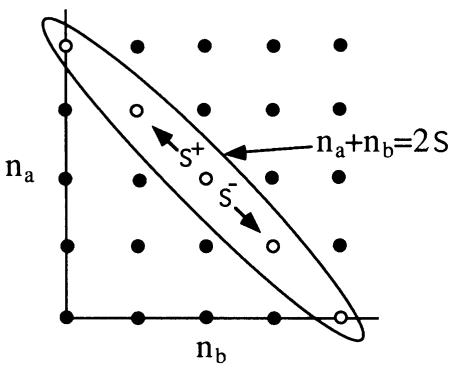
\includegraphics[width=0.5\textwidth]{fig7_1.jpg}
\caption{Schwinger 玻色子 Fock 空间中自旋 $S$ 的投影子空间。}
\label{fig:7.1}
\end{figure}

Schwinger 玻色子便于计算自旋算符的矩阵元：由于不含平方根（与 Holstein--Primakoff 玻色子不同），自旋算符在 Fock 态之间的矩阵元像自由玻色子一样因子化。然而这并不必然简化非 Fock 波函数中自旋关联的计算：Hilbert 空间上的局域约束 (7.6) 引入了 $a$、$b$ 占据数之间的关联。

把表示 (7.5) 推广到 $N$ 个“味”，就把 $SU(N)$ 的生成元定义为广义“自旋”，见第 16 章。大 $N$ 推广允许由小参数 $1/N$ 控制的简单平均场理论，将在第 17、18 章综述。大 $N$ 平均场理论由实际上无相互作用的 Bose 准粒子描述，不同味之间的关联被忽略。

Schwinger 玻色子（SB）与 Holstein--Primakoff 玻色子 (7.1)（HP）密切相关。利用约束 (7.7) 消去 $a$ 玻色子，得到对应关系

\begin{equation*}
\begin{array}{ccc}
\text{SB} & & \text{HP}\\
b & \leftrightarrow & b ,\\
a & \leftrightarrow & \sqrt {2 S - n _ {b}} .
\end{array}
\tag{7.11}
\end{equation*}

Schwinger 玻色子在自旋空间中提供对称表示，而 Holstein--Primakoff 玻色子挑出 $S^{z}$ 方向（后者定义其真空）。因此两种表示适合不同的近似方案：HP 用于破缺对称相，SB 用于对称相。

\subsection{自旋转动}

自旋算符是 SU(2) 变换群的生成元。$\mathcal{R}$ 由三个 Euler 角 $\phi, \theta, \chi$ 参数化：

\begin{equation*}
\mathcal {R} = e ^ {i \phi S ^ {z}} e ^ {i \theta S ^ {y}} e ^ {i \chi S ^ {z}}.
\tag{7.12}
\end{equation*}

自旋算符是正规双线性算符（见 A.2 节）。Schwinger 玻色子产生算符作为 SU(2) 中的矢量变换\footnote{见附录 A 的 (A.17)。}：

\begin{align*}
\binom {a ^ {\dagger}} {b ^ {\dagger}} ' & = \mathcal {R} \binom {a ^ {\dagger}} {b ^ {\dagger}} \mathcal {R} ^ {- 1}\\
& = e ^ {i \frac {1}{2} \chi \sigma^ {z}} e ^ {i \frac {1}{2} \theta \sigma^ {y}} e ^ {i \frac {1}{2} \phi \sigma^ {z}} \binom {a ^ {\dagger}} {b ^ {\dagger}}\\
& = \left( \begin{array}{cc} u \, e ^ {i \chi / 2} & v \, e ^ {i \chi / 2} \\ - v ^ {*} e ^ {- i \chi / 2} & u ^ {*} e ^ {- i \chi / 2} \end{array} \right) \binom {a ^ {\dagger}} {b ^ {\dagger}} ,
\tag{7.13}
\end{align*}

其中函数 $u$、$v$ 定义为

\begin{align*}
u ( \theta , \phi ) & = \cos ( \theta / 2 ) \, e ^ {i \phi / 2} ,\\
v ( \theta , \phi ) & = \sin ( \theta / 2 ) \, e ^ {- i \phi / 2} .
\tag{7.14}
\end{align*}

\section{自旋相干态}

自旋相干态是把 (7.12) 的转动算符 $\mathcal{R}$ 作用于最大极化态 $|S, S\rangle$ 得到的一族自旋态：

\begin{align*}
\left| \hat {\Omega} \right\rangle & = \mathcal {R} ( \chi , \theta , \phi ) \left| S, S \right\rangle\\
& = e ^ {i S ^ {z} \phi} e ^ {i S ^ {y} \theta} e ^ {i S ^ {z} \chi} \left| S, S \right\rangle ,
\tag{7.15}
\end{align*}

其中单位矢量

\begin{equation*}
\hat {\Omega} = \left( \sin \theta \cos \phi \, , \; \sin \theta \sin \phi \, , \; \cos \theta \right)
\tag{7.16}
\end{equation*}

参数化该自旋相干态。我们可以任意定义 $\chi$——这是一种规范自由，可以通过固定 $\chi$ 消去。两个独立角度是“纬度”$\theta$ 与“经度”$\phi$，定义域为

\begin{equation*}
\{ \theta \in [ 0, \pi ] \, , \; \phi \in [ - \pi , \pi ) \}.
\tag{7.17}
\end{equation*}

利用 (7.13)，Schwinger 玻色子变换到转动坐标系 $a \rightarrow a_{\theta,\phi}'$，给出相干态的显式表示：

\begin{align*}
\left| \hat {\Omega} \right\rangle & = e ^ {i S \chi} \, \frac {\left( a ^ {\dagger '} \right) ^ {2 S}}{\sqrt {( 2 S ) !}} \left| 0 \right\rangle = e ^ {i S \chi} \, \frac {\left( u \, a ^ {\dagger} + v \, b ^ {\dagger} \right) ^ {2 S}}{\sqrt {( 2 S ) !}} \left| 0 \right\rangle\\
& = e ^ {i S \chi} \sqrt {( 2 S ) !} \, \sum_ {m} \frac {u ^ {S + m} v ^ {S - m}}{\sqrt {( S + m ) ! \, ( S - m ) !}} \left| S, m \right\rangle ,
\tag{7.18}
\end{align*}

其中 $u$、$v$ 已在 (7.14) 定义。

利用 (7.18) 可以计算任意两个相干态的交叠：

\begin{align*}
\langle \hat {\Omega} | \hat {\Omega} ' \rangle & = e ^ {- i S ( \chi - \chi ' )} \left( u ^ {*} u ' + v ^ {*} v ' \right) ^ {2 S}\\
& = \left( \frac {1 + \hat {\Omega} \cdot \hat {\Omega} '}{2} \right) ^ {S} e ^ {- i S \psi}\\
\psi & = 2 \arctan \left[ \tan \left( \frac {\phi - \phi '}{2} \right) \frac {\cos \left[ \frac {1}{2} ( \theta + \theta ' ) \right]}{\cos \left[ \frac {1}{2} ( \theta - \theta ' ) \right]} \right] + \chi - \chi ' ,
\tag{7.19}
\end{align*}

其中 $\chi, \chi'$ 依赖规范约定。

如 (7.19) 所示，相干态并不正交。现在证明它们张成自旋 $S$ 的态空间。群参数上的积分测度定义为

\begin{equation*}
\frac {2 S + 1}{4 \pi} d \hat {\Omega} = \frac {2 S + 1}{4 \pi} d \theta \sin \theta \, d \phi .
\tag{7.20}
\end{equation*}

这是 SU(2) Lie 群的 Haar 测度。利用这一测度，单位分解由积分\footnote{{$\theta$} 积分的计算见 7.3.1 小节。}给出

\begin{align*}
& \frac {2 S + 1}{4 \pi} \int d \hat {\Omega} \left| \hat {\Omega} \right\rangle \left\langle \hat {\Omega} \right|\\
& = \frac {( 2 S + 1 )}{2} \int_ {- 1} ^ {1} d \cos \theta \, \sum_ {m} \left( \frac {1 + \cos \theta}{2} \right) ^ {S + m} \left( \frac {1 - \cos \theta}{2} \right) ^ {S - m}\\
& \quad \times \frac {( 2 S ) !}{( S + m ) ! ( S - m ) !} \left| S, m \right\rangle \left\langle S, m \right|\\
& = \sum_ {m} \left| S, m \right\rangle \left\langle S, m \right| = I .
\tag{7.21}
\end{align*}

因此相干态构成一个超完备基底。

用同样方式还可证明另一个有用关系\footnote{见习题 3。}

\begin{equation*}
\frac {( S + 1 ) ( 2 S + 1 )}{4 \pi} \int d \hat {\Omega} \, \hat {\Omega} ^ {\alpha} \left| \hat {\Omega} \right\rangle \left\langle \hat {\Omega} \right| = \mathbf {S} ^ {\alpha} \, , \quad \alpha = x, y, z.
\tag{7.22}
\end{equation*}

上述关系容易推广到多自旋。考虑 $\mathcal{N}$ 个格点上自旋的格子，格点记作 $i$。多自旋相干态是单自旋态的乘积：

\begin{equation*}
\left| \hat {\Omega} \right\rangle = \prod_ {i = 1} ^ {\mathcal {N}} \left| \hat {\Omega} _ {i} \right\rangle .
\tag{7.23}
\end{equation*}

其交叠为

\begin{equation*}
\langle \hat {\Omega} | \hat {\Omega} ' \rangle = \prod_ {i} \left( \frac {1 + \hat {\Omega} _ {i} \cdot \hat {\Omega} _ {i} '}{2} \right) ^ {S} e ^ {- i S \sum_ {i} \psi [ \hat {\Omega} _ {i}, \hat {\Omega} _ {i} ' ]}.
\tag{7.24}
\end{equation*}

乘积空间中的单位分解为

\begin{equation*}
\int \prod_ {i} \left( \frac {2 S + 1}{4 \pi} d \hat {\Omega} _ {i} \right) \left| \hat {\Omega} \right\rangle \left\langle \hat {\Omega} \right| = I.
\tag{7.25}
\end{equation*}

任何波函数 $\Psi$ 的自旋关联都可以用积分计算：

\begin{align*}
\frac {\langle \Psi | \mathbf {S} _ {i} \cdot \mathbf {S} _ {j} | \Psi \rangle}{\langle \Psi | \Psi \rangle} & = \frac {( S + 1 - \delta_ {ij} ) ( S + 1 )}{Z} \int \prod_ {i} d \hat {\Omega} _ {i} \left| \Psi [ \hat {\Omega} ] \right| ^ {2} \hat {\Omega} _ {i} \cdot \hat {\Omega} _ {j} ,\\
Z & = \int \prod_ {i} d \hat {\Omega} _ {i} \left| \Psi [ \hat {\Omega} ] \right| ^ {2} ,
\tag{7.26}
\end{align*}

这里用到了 (7.22)。表示 $\Psi[\hat{\Omega}]=\langle\Psi|\hat{\Omega}\rangle$ 是连续的（像 Schrödinger 波函数一样），习题 4 将证明所有自旋算符都表示为变量 $u(\theta,\phi)$、$v(\theta,\phi)$ 的微分算符。自旋相干态可用于计算任何算符的迹。若 $|n\rangle$ 是任意正交归一基，则

\begin{align*}
\operatorname{Tr} \mathcal {O} & = \sum_ {n} \langle n | \mathcal {O} | n \rangle\\
& = \left( \frac {2 S + 1}{4 \pi} \right) ^ {2} \int d \hat {\Omega} \int d \hat {\Omega} ' \sum_ {n} \langle n | \hat {\Omega} \rangle \langle \hat {\Omega} | \mathcal {O} | \hat {\Omega} ' \rangle \langle \hat {\Omega} ' | n \rangle\\
& = \frac {2 S + 1}{4 \pi} \int d \hat {\Omega} \, \langle \hat {\Omega} | \mathcal {O} | \hat {\Omega} \rangle .
\tag{7.27}
\end{align*}

相干态阐明了经典自旋与量子自旋之间的对应。经典极限由 $S \rightarrow \infty$ 得到。在该极限下，由 (7.24)，不同相干态的交叠随 $S$ 指数消失；自旋算符的期望值成为单位矢量的函数，与经典自旋毫无二致。量子效应因此与相干态的非正交性相联系——这也意味着 $\Psi[\hat{\Omega}]$ 在 $\hat{\Omega}$ 空间中有有限宽度。

\subsection{$\theta$ 积分}

把 (7.21) 中的 $\theta$ 积分定义为

\begin{equation*}
I _ {S, m} = \frac {1}{2} \int_ {0} ^ {\pi} d \theta \sin \theta \left( \frac {1 + \cos \theta}{2} \right) ^ {S + m} \left( \frac {1 - \cos \theta}{2} \right) ^ {S - m}.
\tag{7.28}
\end{equation*}

换积分变量

\begin{equation*}
x = \frac {\cos \theta + 1}{2} ,
\tag{7.29}
\end{equation*}

可以证明

\begin{align*}
I _ {S, m} & = \int_ {0} ^ {1} d x \, x ^ {S + m} ( 1 - x ) ^ {S - m}\\
& = ( S + m )! \, ( S - m )! \, / \, ( 2 S + 1 )! .
\tag{7.30}
\end{align*}

验证方法是构造生成函数

\begin{equation*}
f _ {S} ( z ) = \sum_ {n = 0} ^ {2 S} \frac {( 2 S ) !}{( 2 S - n )! \, n !} \, I _ {S, n - S} \, z ^ {n}.
\tag{7.31}
\end{equation*}

把 (7.30) 代入 (7.31) 并用二项式展开：

\begin{align*}
( 2 S + 1 ) f _ {S} ( z ) & = ( z ^ {2 S + 1} - 1 ) / ( z - 1 )\\
& = 1 + z + \ldots + z ^ {2 S} .
\tag{7.32}
\end{align*}

由 (7.31)，$I_{S,m}$ 正是 $f_{S}(z)$ 中 $z^{m + S}$ 的系数，这就证明了 (7.30)。

\begin{exercises}

\item 直接从定义 (7.15) 验证 $|\hat{\Omega}\rangle$ 是 $\hat{\Omega}$ 方向自旋分量的本征态：

\begin{equation*}
\hat {\Omega} \cdot \mathbf {S} \left| \hat {\Omega} \right\rangle = S \left| \hat {\Omega} \right\rangle .
\tag{7.33}
\end{equation*}

提示：利用三个自旋算符 $(S^{x}, S^{y}, S^{z})$ 的 $O(3)$（矢量）变换性质。

\item 利用 (7.33)，证明 Heisenberg 模型在相干态中的期望值为

\begin{equation*}
H [ \hat {\Omega} ] = \langle \hat {\Omega} | \mathcal {H} | \hat {\Omega} \rangle = \frac {S ^ {2}}{2} \sum_ {i, j} J _ {ij} \, \hat {\Omega} _ {i} \cdot \hat {\Omega} _ {j}.
\tag{7.34}
\end{equation*}

提示：对每个自旋，把它的分量写成 $\hat{\Omega}$ 方向的分量与两个横向分量。

\item 循 (7.21) 的推导，证明恒等式 (7.22)。

\item 证明对单自旋的任意波函数，下列关系成立：

\begin{align*}
\langle \Psi | S ^ {+} | \hat {\Omega} \rangle & = v \, \partial_ {u} \Psi ( \hat {\Omega} ) ,\\
\langle \Psi | S ^ {-} | \hat {\Omega} \rangle & = u \, \partial_ {v} \langle \Psi | \hat {\Omega} \rangle ,\\
\langle \Psi | S ^ {z} | \hat {\Omega} \rangle & = \frac {1}{2} \left( u \, \partial_ {u} - v \, \partial_ {v} \right) \Psi ( \hat {\Omega} ) .
\tag{7.35}
\end{align*}

\item 给定微分算符

\begin{equation*}
\mathcal {T} = \sum_ {klj} T _ {klj} \, \partial_ {u} ^ {k} \partial_ {v} ^ {l} u ^ {k + j} v ^ {l - j} ,
\tag{7.36}
\end{equation*}

它在任意两个自旋 $S$ 波函数之间的矩阵元为

\begin{equation*}
\langle \Psi | \mathcal {T} | \Psi ' \rangle = \frac {2 S + 1}{4 \pi} \int d \hat {\Omega} \, \Psi ^ {*} ( \hat {\Omega} ) \left[ \mathcal {T} _ {u, v} \Psi ' ( \hat {\Omega} ) \right].
\tag{7.37}
\end{equation*}

证明可以通过代入

\begin{equation*}
\langle \Psi | \mathcal {T} | \Psi ' \rangle = \frac {2 S + 1}{4 \pi} \int d \hat {\Omega} \, \Psi ^ {*} ( \hat {\Omega} ) \, T [ u ^ {*}, v ^ {*}, u, v ] \, \Psi ' ( \hat {\Omega} ) ,
\tag{7.38}
\end{equation*}

来计算 (7.37)，其中

\begin{equation*}
T \left[ u ^ {*}, v ^ {*}, u, v \right] = \sum_ {klj} C _ {kl} \, T _ {klj} \, u ^ {*k} v ^ {*l} u ^ {k + j} v ^ {l - j}
\tag{7.39}
\end{equation*}

而

\begin{equation*}
C _ {kl} = \prod_ {m = 2} ^ {k + l + 1} ( 2 S + m ).
\tag{7.40}
\end{equation*}

提示：把 $\Psi$、$\Psi'$ 展开成 $u, v$ 的二项式，对 (7.37) 与 (7.40) 先积 $d\phi$ 再积 $d\theta$。

\end{exercises}

\begin{chapbib}
\item Holstein--Primakoff 算符定义于
  T. Holstein and H. Primakoff, Phys. Rev. \textbf{58}, 1908 (1940)。
\item Schwinger 玻色子的定义及其在 Clebsch--Gordan 系数计算中的应用：
  J. Schwinger, \textit{Quantum Theory of Angular Momentum}, edited by L. Biedenharn and H. Van Dam (Academic, New York, 1965)。
\item 自旋相干态及其推广见
  A. Perelomov, \textit{Generalized Coherent States and Their Applications} (Springer-Verlag, New York, 1986)；
  J. R. Klauder and B. Skagerstam, \textit{Coherent States} (World Scientific, 1985)。
\item 自旋相干态与半经典近似的联系见
  J. Klauder, Phys. Rev. D \textbf{19}, 2349 (1979)。
\item 相干态在量子 Heisenberg 铁磁体中的应用见
  F. D. M. Haldane, Phys. Rev. Lett. \textbf{57}, 1488 (1986)。
\end{chapbib}

% 第8章 变分波函数与母哈密顿量
\chapter{变分波函数与母哈密顿量}

对大多数非铁磁 Heisenberg 模型，我们并不知道其基态。即使是解析形式已知的那些（如一维 Bethe 解），其自旋关联也需要数值计算。变分波函数为基态提供了有根据的猜测。通过相对于选定参数集极小化能量的变分计算，可以获得物理洞察。变分途径把我们带到任何特定展开方案——半经典的、大 $N$ 的或其他——的适用范围之外。如 Hubbard 模型的情形所示（见 4.1 节），变分途径的首要优点是概念简单明了。

这里我们把变分波函数与“母哈密顿量”（parent Hamiltonian）的概念联系起来。母哈密顿量是使某个特定波函数恰好成为其精确基态的哈密顿量。虽然该哈密顿量可能因额外的相互作用而不同于物理模型，但它有助于加深对后者的理解，揭示相互作用与基态关联之间的关系。把母哈密顿量方法扩展到理解激发，是第 9 章的主题。

如文献注释所示，变分态与母哈密顿量的方法论很大程度上为其他高度关联的量子体系所共有。特别地，本章的方法与分数量子霍尔效应的著名处理极为类似。

\section{价键态}

价键态是反铁磁 Heisenberg 模型的变分波函数，在量子磁学与高温超导的语境下已被广泛研究。其一般形式为

\begin{equation*}
\left| \{c _ {\alpha} \}, S \right\rangle = \sum_ {\alpha} c _ {\alpha} \left| \alpha \right\rangle ,
\tag{8.1}
\end{equation*}

\begin{figure}[H]
\centering
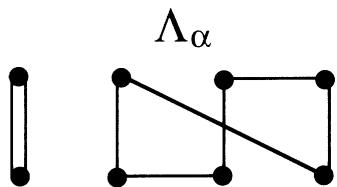
\includegraphics[width=0.5\textwidth]{fig8_1.jpg}
\caption{$S = 1$ 的一个价键组态。}
\label{fig:8.1}
\end{figure}

其中 $c_{\alpha}$ 是变分参数，而

\begin{equation*}
\left| \alpha \right\rangle = \prod_ {(ij) \in \Lambda_ {\alpha}} \left( a _ {i} ^ {\dagger} b _ {j} ^ {\dagger} - b _ {i} ^ {\dagger} a _ {j} ^ {\dagger} \right) \left| 0 \right\rangle .
\tag{8.2}
\end{equation*}

$a_{i}, b_{i}$ 是格点 $i$ 上的 Schwinger 玻色子\footnote{见 7.2 节。}。$\Lambda_{\alpha}$ 是格子上键 $(ij)$ 的一个特定组态，如图~\ref{fig:8.1} 所示。对 $\Lambda_{\alpha}$ 的条件是：恰好 $2S$ 条键从每个格点发出。某些情形下，大幅子极限中 (8.1) 的求和由有限数目的组态主导。而 (8.1) 中含有宏观多组态的情形，被 Anderson 称为“共振价键态”（RVB）。

由 (7.13) 容易验证，所有键算符 $a_i^\dagger b_j^\dagger - b_i^\dagger a_j^\dagger$ 在整体自旋转动下不变。因此 $|\{c_\alpha\}, S\rangle$ 是总自旋单态。价键态的一个特殊类由

\begin{equation*}
\left| \hat {u}, S \right\rangle = \sum_ {\alpha} \left( \prod_ {(ij) \in \alpha} u _ {ij} \right) \left| \alpha \right\rangle .
\tag{8.3}
\end{equation*}

给出，其中独立变分参数 $u_{ij}$ 至多 $\mathcal{N}(\mathcal{N}-1)/2$ 个，$\mathcal{N}$ 是格点数。

若键参数是二分的且为正：

\begin{equation*}
u _ {ij} = \left\{ \begin{array}{ll} u _ {ij} > 0 & i \in A \text{ 且 } j \in B \\ 0 & i, j \text{ 在同一子晶格} \end{array} \right. ,
\tag{8.4}
\end{equation*}

则 (8.3) 满足 Marshall 符号判据 (5.13)——这正是二分 Heisenberg 反铁磁体基态所要求的。

Schwinger 玻色子平均场态定义为

\begin{equation*}
\left| \hat {u} \right\rangle = \exp \left[ \frac {1}{2} \sum_ {ij} u _ {ij} \left( a _ {i} ^ {\dagger} b _ {j} ^ {\dagger} - b _ {i} ^ {\dagger} a _ {j} ^ {\dagger} \right) \right] \left| 0 \right\rangle ,
\tag{8.5}
\end{equation*}

其中 $u_{ij} = -u_{ji}$。这类态由 Heisenberg 反铁磁体的 Schwinger 玻色子平均场理论产生（见第 18 章）。$|\hat{u}\rangle$ 包含各个格点上不同自旋大小的贡献，因此并不是真正的自旋态。对 Schwinger 玻色子作 Bogoliubov 变换，可把它变成可因子化的 Fock 态（实际上是变换后玻色子的真空）。如习题所示，平均场态的关联可以解析求出。价键态 $|\hat{u}, S\rangle$ 可由 (8.5) 经 (7.7) 的 $P_{S}$ 投影构造：

\begin{equation*}
\left| \hat {u}, S \right\rangle = P _ {S} \left| \hat {u} \right\rangle .
\tag{8.6}
\end{equation*}

但由于 $P_{S}$ 引入的关联，投影后的态不再可因子化。

计算 $|\hat{u}\rangle$ 中的关联远比 $|\hat{u}, S\rangle$ 容易。可用于计算价键态自旋关联的方法多种多样：有数值方法（组合计算或对波函数作 Monte Carlo 抽样）；有用自旋相干态表示的精确计算（见 8.3.1 小节）；还有 $1/N$ 展开（$N$ 为 Schwinger 玻色子味的数目）。矩阵 $\{\hat{u}\}$ 的整体大小固定为每格点平均 $2S$ 个玻色子。平均场态 $|\hat{u}\rangle$ 的自旋关联是该展开的零阶近似；通过对受约束的生成泛函作 $1/N$ 展开，可系统地改进之——与第 16 章配分函数的大 $N$ 展开极为类似。这些方法的例子见文献注释。

某些价键态是已知“母”哈密顿量的精确基态。下面描述投影算符技术，它对构造母哈密顿量普遍有用\footnote{Haldane 曾用投影算符方法论证分数量子霍尔效应的 Laughlin 波函数，见文献注释。}。

\section{$S = \frac{1}{2}$ 态}

任何格点上 $S = \frac{1}{2}$ 的态用旋量态标记：

\begin{equation*}
\left| \uparrow_{i} \right\rangle \equiv a _ {i} ^ {\dagger} \left| 0 \right\rangle \, , \quad \left| \downarrow_{i} \right\rangle \equiv b _ {i} ^ {\dagger} \left| 0 \right\rangle .
\tag{8.7}
\end{equation*}

\begin{figure}[H]
\centering
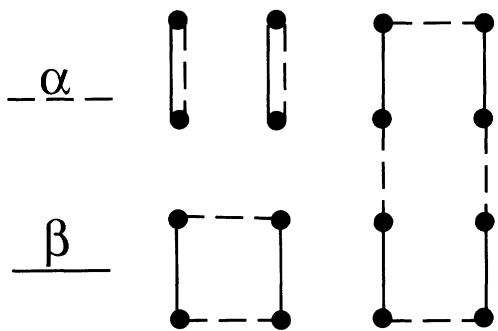
\includegraphics[width=0.5\textwidth]{fig8_2.jpg}
\caption{两个价键组态的交叠（$S = \frac{1}{2}$）。}
\label{fig:8.2}
\end{figure}

任何满足 Marshall 符号的二分价键组态 (8.2) 都可以写成归一化的单态键乘积：

\begin{equation*}
\left| \alpha \right\rangle_{S = \frac {1}{2}} = \prod_{(ij) \in \Lambda_ {\alpha}}^ {i \in A, \, j \in B} \left( \left| \uparrow_{i} \right\rangle \left| \downarrow_{j} \right\rangle - \left| \downarrow_{i} \right\rangle \left| \uparrow_{j} \right\rangle \right) / \sqrt {2}.
\tag{8.8}
\end{equation*}

(8.8) 的自旋关联简单地为

\begin{equation*}
\langle \mathbf {S} _ {i} \mathbf {S} _ {j} \rangle = \left\{ \begin{array}{ll} \frac {3}{4} & i = j \\ - \frac {3}{4} & (ij) \in \Lambda_ {\alpha} \\ 0 & (ij) \notin \Lambda_ {\alpha} \end{array} \right. .
\tag{8.9}
\end{equation*}

于是，若 $\Lambda_{\alpha}$ 中的键是短程的，$|\alpha\rangle_{S=\frac{1}{2}}$ 是无序的“自旋液体”态。不同价键组态彼此不正交，其有限交叠由\footnote{见 Sutherland，文献注释。}

\begin{align*}
\langle \alpha | \beta \rangle & = \prod_{l \in \langle \alpha | \beta \rangle} 2 ^ {1 - L _ {l} / 2}\\
& = 2 ^ {N _ {L} ^ {\langle \alpha \beta \rangle} - \mathcal {N}} ,
\tag{8.10}
\end{align*}

给出。第一行是对两个组态交叠中出现的所有长度为 $L_{l}$ 的回路 $l$ 求积。交叠可以把两个价键组态叠在一起画出，如图~\ref{fig:8.2}。$\alpha$ 与 $\beta$ 中两条相同的键产生长度 $L = 2$ 的回路。(8.10) 第二行中 $N_{L}$ 是回路总数，$\mathcal{N}$ 是格子上的格点数。

\begin{figure}[H]
\centering
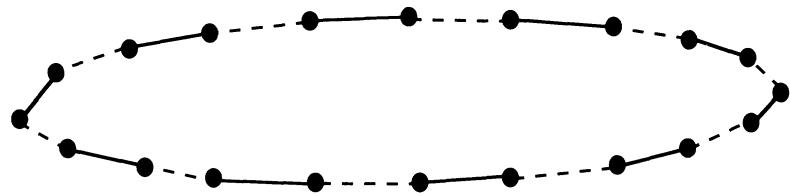
\includegraphics[width=0.55\textwidth]{fig8_3.jpg}
\caption{两个二聚体态 $|d\rangle_{\pm}$，分别用实线与虚线画出。}
\label{fig:8.3}
\end{figure}

由于 $|\alpha\rangle$ 每格点含一条键，而所有简单格子的配位数大于等于二，$|\alpha\rangle$ 破缺格子平移对称。在 (8.1) 中对 $\alpha$ 求和可以恢复这一对称。

以下我们把自己限于近邻键或“二聚体”的价键态。一维与二维情形分别讨论。

\subsection{Majumdar--Ghosh 哈密顿量}

Majumdar 与 Ghosh 引入哈密顿量

\begin{equation*}
H ^ {\mathrm{MG}} = \frac {4 | K |}{3} \sum_ {i = 1} ^ {\mathcal {N}} \left( \mathbf {S} _ {i} \cdot \mathbf {S} _ {i + 1} + \frac {1}{2} \mathbf {S} _ {i} \cdot \mathbf {S} _ {i + 2} \right) + \frac {1}{2} \mathcal {N} ,
\tag{8.11}
\end{equation*}

$i$ 标记偶数格点数的一维链的格点，$S_{\mathcal{N}+1} = S_{1}$。下面将看到，$H^{\mathrm{MG}}$ 是图~\ref{fig:8.3} 所画两个二聚体态的母哈密顿量：

\begin{equation*}
\left| d \right\rangle_{\pm} = \prod_ {n = 1} ^ {\mathcal {N}/2} \left( \left| \uparrow_{2n} \right\rangle \left| \downarrow_{2n \pm 1} \right\rangle - \left| \downarrow_{2n} \right\rangle \left| \uparrow_{2n \pm 1} \right\rangle \right) / \sqrt {2}.
\tag{8.12}
\end{equation*}

我们将证明

\begin{equation*}
H ^ {\mathrm{MG}} \left| d \right\rangle_{\pm} = 0 ,
\tag{8.13}
\end{equation*}

且所有其他本征能量为正。于是 $|d\rangle_{\pm}$ 张成 $H^{\mathrm{MG}}$ 的基态流形。$H^{\mathrm{MG}}$ 包含次近邻间的反铁磁相互作用，部分阻挫了近邻关联。因此可以预期基态比纯近邻模型更无序。的确，近邻模型 Bethe 波函数的关联按距离的负幂衰减，而由 (8.9)，二聚体态的关联超出一个格点常量即为零。

(8.13) 的证明富有启发性，因为它演示了构造母哈密顿量的一般技术。格点 $(i-1, i, i+1)$ 上三自旋的总自旋为

\begin{equation*}
\mathbf {J} _ {i} = \mathbf {S} _ {i - 1} + \mathbf {S} _ {i} + \mathbf {S} _ {i + 1} ,
\tag{8.14}
\end{equation*}

其平方具有本征值 $J(J + 1)$，$J = \frac{1}{2}, \frac{3}{2}$。基本思想是把 $H^{\mathrm{MG}}$ 表为投影算符之和：

\begin{equation*}
H ^ {\mathrm{MG}} = | K | \sum_ {i} \mathcal {P} _ {3/2} ( i - 1, i, i + 1 ) ,
\tag{8.15}
\end{equation*}

其中

\begin{align*}
\mathcal {P} _ {3/2} ( i - 1, i, i + 1 ) & = \frac {1}{3} \left( \mathbf {J} _ {i} ^ {2} - \frac {3}{4} \right)\\
& = \frac {1}{2} + \frac {2}{3} \left( \mathbf {S} _ {i - 1} \cdot \mathbf {S} _ {i} + \mathbf {S} _ {i - 1} \cdot \mathbf {S} _ {i + 1} + \mathbf {S} _ {i} \cdot \mathbf {S} _ {i + 1} \right) .
\tag{8.16}
\end{align*}

显然，$\mathcal{P}_{3/2}$ 湮灭三自旋组 $(i-1, i, i+1)$ 总自旋 $J = \frac{1}{2}$ 的任何态。另外，二聚体态 (8.12) 不含任何三个格点总 $J^{z} > \frac{1}{2}$ 的分量，因为三个自旋中有两个的 $S^{z}$ 量子数相消。

这蕴含不存在总自旋 $J > \frac{1}{2}$ 的三自旋组，论证如下：假设有一个 $J^{z} = \frac{1}{2}$ 但 $J = \frac{3}{2}$ 的三自旋组。对 $|d\rangle$ 作整体转动，这将通过 $J_{i}^{+}$ 的作用把 $J_{i}^{z} = \frac{3}{2}$ 的分量混入波函数，与 $|d\rangle$ 的转动不变性矛盾（见 (8.3) 之前的讨论）。于是 $|d\rangle$ 中不可能有任何 $J > \frac{1}{2}$ 分量，故每个算符 $\mathcal{P}_{3/2}$ 湮灭 $|d\rangle_{\pm}$。由于 $|K|\mathcal{P}_{3/2}$ 是非负算符，$|d\rangle_{\pm}$ 张成 $H^{\mathrm{MG}}$ 的基态流形。证毕。

\subsection{正方格子 RVB 态}

在 $S = \frac{1}{2}$ 的正方格子上，共振价键（RVB）态 (8.3) 满足量子反铁磁体 Marshall 定理 5.1 与 5.2 的一切要求。P. W. Anderson 提出这些态作为自旋液体基态的候选。虽然（各种迹象表明）正方格子上的近邻反铁磁体在 $T = 0$ 是有序的，这些态在掺杂反铁磁体与高温超导的语境下非常流行（见文献注释与第 19 章）。

遗憾的是，RVB 态的关联不易计算。由 (8.10) 可见其分量 $|\alpha\rangle$ 并不正交。正方格子上不同键覆盖的数目随格点数指数增长。M. E. Fisher 曾计算（见文献注释）大小为 $\mathcal{N}$ 的正方格子上二聚体组态的数目增长为

\begin{equation*}
\text{二聚体组态数} \sim ( 1.791623 ) ^ {\mathcal {N}/2}.
\tag{8.17}
\end{equation*}

Liang、Douçot 与 Anderson 在有限格子上的数值 Monte Carlo 模拟表明，若键至少按

\begin{equation*}
u _ {ij} \propto \left| \mathbf {x} _ {i} - \mathbf {x} _ {j} \right| ^ {- p} \, , \quad p \geq 5
\tag{8.18}
\end{equation*}

衰减，RVB 态便没有长程序。因此 RVB 态既可用作有序相、也可用作无序相的变分基态，这使它们成为研究从 Néel 反铁磁体到顺磁相转变的诱人候选。

\section{价键固体与 AKLT 模型}

价键固体（VBS）是

\begin{equation*}
\left| \Psi^ {\mathrm{VBS}} \right\rangle = \prod_{\langle ij \rangle} \left( a _ {i} ^ {\dagger} b _ {j} ^ {\dagger} - b _ {i} ^ {\dagger} a _ {j} ^ {\dagger} \right) ^ {M} \left| 0 \right\rangle ,
\tag{8.19}
\end{equation*}

其中 $\langle ij\rangle$ 是格子的所有近邻键，整数 $M$ 满足

\begin{equation*}
M = 2 S / z.
\tag{8.20}
\end{equation*}

$z$ 是格子配位数。显然 (8.20) 使 $S$ 的取值依赖于格子结构：例如一维格子 $S = 1, 2 \ldots$，正方格子 $S = 2, 4 \ldots$。若干 VBS 态画于图~\ref{fig:8.4}。

\begin{figure}[H]
\centering
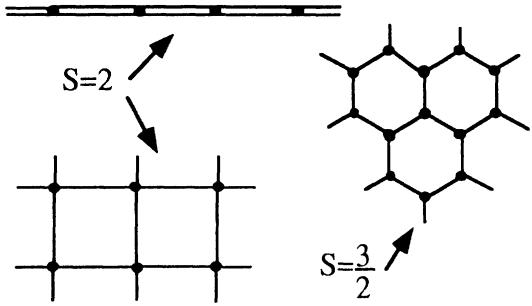
\includegraphics[width=0.55\textwidth]{fig8_4.jpg}
\caption{若干价键固体。}
\label{fig:8.4}
\end{figure}

Affleck、Kennedy、Lieb 与 Tasaki（AKLT）为 VBS 态构造了母哈密顿量：

\begin{equation*}
\mathcal {H} ^ {\mathrm{AKLT}} = \sum_{\langle ij \rangle} \sum_{J = 2S - M + 1} ^ {2S} K _ {J} \, \mathcal {P} _ {J} ( ij ) \, , \quad K _ {J} \geq 0.
\tag{8.21}
\end{equation*}

键投影算符 $\mathcal{P}_{J}(ij)$ 把键自旋 $J_{ij} = S_{i} + S_{j}$ 投影到大小为 $J$ 的子空间。$m = 0, 1, 2, \ldots$ 次幂的 $S_{i} \cdot S_{j}$ 的任何幂次都可以用 $J_{ij}^{2}$ 的幂写出，并展开为键投影算符的线性组合：

\begin{equation*}
\left( \mathbf {S} _ {i} \cdot \mathbf {S} _ {j} \right) ^ {m} = \sum_ {J = 0} ^ {2 S} \left[ \frac {1}{2} J ( J + 1 ) - S ( S + 1 ) \right] ^ {m} \mathcal {P} _ {J} ( ij ).
\tag{8.22}
\end{equation*}

反过来，(8.22) 可以反解，把键投影算符表示为 $\mathbf{S}_i\cdot \mathbf{S}_j$ 的多项式。

为证明 (8.19) 是 (8.21) 的基态，我们证明

\begin{equation*}
\mathcal {H} ^ {\mathrm{AKLT}} \left| \Psi^ {\mathrm{VBS}} \right\rangle = 0 ,
\tag{8.23}
\end{equation*}

这在 $|\Psi^{\mathrm{VBS}}\rangle$ 对任何 $(ij)$ 都不含键自旋 $J(ij) > 2S - M$ 的分量时成立。

考虑对 $\left|\Psi^{\mathrm{VBS}}\right\rangle$ 的如下贡献——特定键 $(ij)$ 上 $a^{\dagger}$ 个数取最大可能值的项：

\begin{equation*}
\dots \left( a _ {i} ^ {\dagger} \right) ^ {2S - M} \left( a _ {i} ^ {\dagger} b _ {j} ^ {\dagger} - b _ {i} ^ {\dagger} a _ {j} ^ {\dagger} \right) ^ {M} \left( a _ {j} ^ {\dagger} \right) ^ {2S - M} \dots .
\tag{8.24}
\end{equation*}

数一下键上 $a^{\dagger}$ 与 $b^{\dagger}$ 个数之差，发现 (8.19) 中 $J_{ij}^{z}$ 的最大本征值为

\begin{equation*}
J _ {\mathrm{max}} ^ {z} = 2 S - M.
\tag{8.25}
\end{equation*}

若 $\left|\Psi^{\mathrm{VBS}}\right\rangle$ 含有键自旋 $J > J_{max}^{z}$ 的分量，则对整个波函数作整体转动将产生 $J^{z'} = J$ 的分量；但 $\left|\Psi^{\mathrm{VBS}}\right\rangle$ 在整体转动下不变，与 (8.25) 矛盾。于是 $J_{max} = 2S - M$，我们证明了 $\left|\Psi^{\mathrm{VBS}}\right\rangle$ 被 $H^{\mathrm{AKLT}}$ 湮灭——后者只含 $J > J_{max}$ 的投影算符。由于 (8.21) 中 $K_{J}$ 非负，$H^{\mathrm{AKLT}}$ 的本征值非负，$\left|\Psi^{\mathrm{VBS}}\right\rangle$ 是一个基态。证毕。

一个重要例子是自旋 1 链：$S = 1$、$M = 1$。由 (8.22)，哈密顿量的显式形式为

\begin{align*}
\mathcal {H} ^ {\mathrm{AKLT}} & = K \sum \mathcal {P} _ {2} ( ij )\\
& = K \sum_{\langle ij \rangle} \left[ \mathbf {S} _ {i} \cdot \mathbf {S} _ {j} + \frac {1}{3} \left( \mathbf {S} _ {i} \cdot \mathbf {S} _ {j} \right) ^ {2} + \frac {2}{3} \right].
\tag{8.26}
\end{align*}

这一模型在标准 Heisenberg 模型上加了一个双二次项。我们将看到，该模型的基态和激发与用其他方法对标准 Heisenberg 模型预言的相似。就此而言，可以断定双二次微扰实际上是“小”的。

\subsection{价键固体中的关联}

为计算 VBS 态 (8.19) 的关联，利用 (7.18) 定义的自旋相干态 $|\hat{\Omega}\rangle$。这一基底使我们能把 VBS 关联表达为经典统计力学平均。

VBS 态与自旋相干态的交叠为

\begin{align*}
\Psi^ {\mathrm{VBS}} [ \hat {\Omega} ] & = \langle 0 | \prod_{\langle ij \rangle} \left( a _ {i} b _ {j} - b _ {i} a _ {j} \right) ^ {M} \prod_ {i} \frac {\left( u _ {i} a _ {i} ^ {\dagger} + v _ {i} b _ {i} ^ {\dagger} \right) ^ {2S}}{\sqrt {( 2 S ) !}} \left| 0 \right\rangle\\
& = \sqrt {( 2 S ) !} \prod_{\langle ij \rangle} \left( u _ {i} v _ {j} - v _ {i} u _ {j} \right) ^ {M}\\
& = \sqrt {( 2 S ) !} \prod_{\langle ij \rangle} \left( \frac {1 - \hat {\Omega} _ {i} \cdot \hat {\Omega} _ {j}}{2} \right) ^ {M/2} ,
\tag{8.27}
\end{align*}

其中 $u(\theta,\phi)$、$v(\theta,\phi)$ 已在 (7.14) 定义。用单位矢量显式表达的 VBS 波函数对理解其关联极为有用。由 (7.26)，自旋关联为

\begin{align*}
\langle \mathbf {S} _ {i} \cdot \mathbf {S} _ {j} \rangle & = Z ^ {- 1} ( S + 1 - \delta_ {ij} ) ( S + 1 )\\
& \quad \times \int \prod_ {i} d \hat {\Omega} _ {i} \left| \Psi^ {\mathrm{VBS}} [ \hat {\Omega} ] \right| ^ {2} \hat {\Omega} _ {i} \cdot \hat {\Omega} _ {j} ,
\tag{8.28}
\end{align*}

归一化分母为

\begin{equation*}
Z = \int \prod_ {i} d \hat {\Omega} _ {i} \left| \Psi^ {\mathrm{VBS}} [ \hat {\Omega} ] \right| ^ {2}.
\tag{8.29}
\end{equation*}

对开放的一维格子，(8.28) 可以用迭代程序显式计算\footnote{见 Arovas、Auerbach 与 Haldane，文献注释。}。距离为 $n$ 个格点间隔时结果为

\begin{align*}
\langle \mathbf {S} _ {0} \cdot \mathbf {S} _ {n} \rangle & = \left\{ \begin{array}{ll} ( - 1 ) ^ {n} ( S + 1 ) ^ {2} \exp [ - \kappa | n | ] & n \neq 0 \\ S ( S + 1 ) & n = 0 \end{array} \right. ,\\
\kappa ( S ) & = \ln \left( 1 + \frac {2}{S} \right) .
\tag{8.30}
\end{align*}

关联的大小以纯指数方式衰减。后续章节我们将看到，这一行为类似于第 12、13 章综述的 Haldane 连续近似对 Heisenberg 反铁磁体的预言。这支持了我们此前的论断：(8.26) 与标准 Heisenberg 模型相距不“远”。

对更高维，可以通过考虑一个等价的经典统计力学体系来理解关联。定义经典 Boltzmann 权重

\begin{equation*}
\exp \left( - \frac {\Phi}{T} \right) \Leftrightarrow \left| \Psi^ {\mathrm{VBS}} [ \hat {\Omega} ] \right| ^ {2} ,
\tag{8.31}
\end{equation*}

其中有效“温度”为

\begin{equation*}
T \Leftrightarrow \frac {1}{M} ,
\tag{8.32}
\end{equation*}

经典“能量”由在 Néel 关联附近（即 $(1 + \hat{\Omega}_{i} \cdot \hat{\Omega}_{j})$ 小值处）展开得到：

\begin{align*}
\Phi & = - \sum_{\langle ij \rangle} \ln \left[ ( 1 - \hat {\Omega} _ {i} \cdot \hat {\Omega} _ {j} ) / 2 \right]\\
& \approx \sum_{\langle ij \rangle} \left[ \frac {1}{2} + \frac {1}{2} \left( \hat {\Omega} _ {i} \cdot \hat {\Omega} _ {j} \right) + \mathcal {O} \left( 1 + \hat {\Omega} _ {i} \cdot \hat {\Omega} _ {j} \right) ^ {2} \dots \right] .
\tag{8.33}
\end{align*}

$\Phi$ 是一个类经典 Heisenberg 哈密顿量，具有短程反铁磁相互作用与 $O(3)$ 转动对称。由 Mermin--Wagner 定理 6.2 的经典版本（见 (6.35)），预期有限 $T$（即有限 $M$）下一维、二维无长程序。于是一维、二维格子上的 VBS 态只有短程序，即它们描述“量子自旋液体”。另一方面，在三维格子上，对足够大的 $M$（即低“温度”），预期经典哈密顿量产生长程反铁磁序；此时 VBS 态描述一个转动不变的、但具有真反铁磁长程序的态\footnote{类似的经典类比技巧曾被 Laughlin 用于分数量子霍尔效应，见文献注释。}。

\begin{exercises}

\item 画出线性链、正方、蜂窝、三角与立方格子的价键态。每种格子允许的 $S$ 值是什么？

\item 对二分格子，证明价键固体 (8.19) 满足 Marshall 符号判据 (5.13)。

\item 证明恒等式

\begin{equation*}
\mathcal {P} _ {2} ( ij ) = \mathbf {S} _ {i} \cdot \mathbf {S} _ {j} + \frac {1}{3} \left( \mathbf {S} _ {i} \cdot \mathbf {S} _ {j} \right) ^ {2} + \frac {2}{3}.
\tag{8.34}
\end{equation*}

\item Schwinger 玻色子平均场态中关联的生成泛函由泛函

\begin{equation*}
Z [ j ] = \left\langle \hat {u} \left| \exp \left[ \sum_ {im} a _ {im} ^ {\dagger} j _ {im} a _ {im} \right] \right| \hat {u} \right\rangle .
\tag{8.35}
\end{equation*}

给出。证明

\begin{equation*}
Z [ \hat {j} ] = \det_{im} \left| 1 - \hat {u} e ^ {\hat {j}} \hat {u} e ^ {\hat {j}} \right| ^ {-1/2} ,
\tag{8.36}
\end{equation*}

其中

\begin{equation*}
\hat {j} _ {im, i'm'} \equiv \delta_ {ii '} \delta_ {mm '} j _ {im}.
\tag{8.37}
\end{equation*}

提示：插入用玻色子相干态（见附录 C）表示的单位分解，把 $Z$ 写成复 Gauss 积分。

\item 考虑一维平均场态 $|\hat{u}\rangle$，其中

\begin{equation*}
\hat {u} _ {ij} = u \left( \delta_ {j, i + 1} + \delta_ {j, i - 1} \right).
\tag{8.38}
\end{equation*}

用对角源 $j_{im} = j$ 的 (8.36)，把平均占据数方程写为

\begin{equation*}
n ( u ) = \sum_ {m} \frac {\partial \ln Z [ \hat {j} ]}{\partial j _ {im}} = 2 S.
\tag{8.39}
\end{equation*}

解出函数 $u(S)$。

\item 利用

\begin{equation*}
S _ {i} ^ {z} \equiv \frac {1}{2} \left( n _ {i, \frac {1}{2}} - n _ {i, - \frac {1}{2}} \right),
\tag{8.40}
\end{equation*}

通过把 $Z(j)$ 对适当的源项求导，证明在位平均场涨落为

\begin{equation*}
\frac {\left\langle \hat {u} ^ {\mathrm{VBS}} \left| \left( S _ {i} ^ {z} \right) ^ {2} \right| \hat {u} ^ {\mathrm{VBS}} \right\rangle}{\langle \hat {u} ^ {\mathrm{VBS}} | \hat {u} ^ {\mathrm{VBS}} \rangle} = \frac {1}{2} S ( S + 1 ).
\tag{8.41}
\end{equation*}

利用转动不变性把结果与 $\langle S^{2}\rangle$ 联系起来。忽略局域约束带来的误差是多少？

\item 用 (8.36) 的 $Z(j)$，计算一维价键态的平均场关联函数

\begin{equation*}
\frac {\left\langle \hat {u} ^ {\mathrm{VBS}} \left| S _ {0} ^ {z} S _ {n} ^ {z} \right| \hat {u} ^ {\mathrm{VBS}} \right\rangle}{\langle \hat {u} ^ {\mathrm{VBS}} | \hat {u} ^ {\mathrm{VBS}} \rangle} ,
\tag{8.42}
\end{equation*}

并把结果与 (8.30) 的精确 VBS 关联比较。

\end{exercises}

\begin{chapbib}
\item 本章的若干想法与例子取自
  D. P. Arovas and S. M. Girvin, \textit{Exact Answers to Some Interesting Questions}, Proc. 7th International Conference on Many Body Theories, Minneapolis (1991) 的讲义。
\item AKLT 模型引入于
  I. Affleck, T. Kennedy, E. H. Lieb, and H. Tasaki, Phys. Rev. Lett. \textbf{59}, 799 (1987)。
\item Majumdar--Ghosh 模型定义于
  C. K. Majumdar and D. K. Ghosh, J. Math Phys. \textbf{10}, 1388 (1969)。
\item 一维价键固体的精确关联计算于
  D. P. Arovas, A. Auerbach, and F. D. M. Haldane, Phys. Rev. Lett. \textbf{60}, 531 (1988)。
\item 共振价键及其与高温超导可能的联系由
  P. W. Anderson, Science \textbf{235}, 1196 (1987)；
  S. Kivelson, D. Rokhsar, and J. Sethna, Phys. Rev. B \textbf{35}, 8865 (1987)
  提出。
\item 式 (8.17) 导出于
  M. E. Fisher, Phys. Rev. \textbf{124}, 1664 (1961)。
\item RVB 态关联的计算见
  W. Sutherland, Phys. Rev. B \textbf{37}, 3786 (1988)；
  M. Kohmoto and Y. Shapir, Phys. Rev. Lett. \textbf{61}, 9439 (1988)；
  S. Liang, B. Douçot, and P. W. Anderson, Phys. Rev. Lett. \textbf{61}, 365 (1988)；
  E. Fradkin, \textit{Field Theories of Condensed Matter Systems} (Addison-Wesley, 1991), 第六章。
\item 价键态关联的 $1/N$ 展开完成于
  M. Raykin and A. Auerbach, Phys. Rev. B \textbf{47}, 5118 (1993)。
  发现其低阶结果与精确关联 (8.30) 出人意料地吻合。
\item 投影算符方法在分数量子霍尔效应 Laughlin 波函数上的应用综述于
  F. D. M. Haldane, \textit{The Quantum Hall Effect}, edited by R. E. Prange and S. M. Girvin (Springer-Verlag, 1987), 第八章。
\item 著名的“经典等离子体类比”可以计算分数量子霍尔效应 Laughlin 态的关联，其精神与 (8.31) 十分相似。见
  R. B. Laughlin, Phys. Rev. Lett. \textbf{50}, 1395 (1983)；
  及上引 \textit{The Quantum Hall Effect} 一书第七章。
\end{chapbib}

% 第9章 从基态到激发
\chapter{从基态到激发}

前几章的重点主要在 Heisenberg 模型的基态。知道精确基态——或者退而求其次，一个好的变分态——使我们能够计算 $T = 0$ 的等时自旋关联。然而实验测量的是有限频率、有限温度下的动力学响应。由线性响应理论（见附录 B）显然可知，动力学的关联依赖于激发态与激发能。

本章将用基态关联构造某些近似低激发。这一途径称为单模近似（single mode approximation，SMA）\footnote{SMA 最初由 Bijl 与 Feynman 用于确定超流 ${}^{4}$He 的声子--旋子色散曲线。}。

Heisenberg 反铁磁体为展示具有高度关联基态的体系的 SMA 提供了机会。

自旋激发与关联的信息包含在动力学结构因子 (B.15) 中：

\begin{align*}
S ( \mathbf {q}, \omega ) & = \mathcal {N} ^ {- 1} \int_ {- \infty} ^ {\infty} d t \, e ^ {i \omega t} \sum_ {ij} e ^ {i \mathbf {q} ( \mathbf {X} _ {i} - \mathbf {X} _ {j} )} \langle S _ {i} ^ {z} ( t ) S _ {j} ^ {z} ( 0 ) \rangle\\
& = \frac {2 \pi}{\mathcal {N} Z} \sum_ {\alpha , \beta} e ^ {- E _ {\alpha} / T} \langle \alpha | S _ {\mathbf {q}} ^ {z} | \beta \rangle \langle \beta | S _ {- \mathbf {q}} ^ {z} | \alpha \rangle \, \delta ( \omega + E _ {\alpha} - E _ {\beta} ) .
\tag{9.1}
\end{align*}

等时关联函数为

\begin{align*}
S ( \mathbf {q} ) & = \int_ {- \infty} ^ {+ \infty} \frac {d \omega}{2 \pi} \, S ( \mathbf {q}, \omega )\\
& = \mathcal {N} ^ {- 1} \langle S _ {\mathbf {q}} ^ {z} S _ {- \mathbf {q}} ^ {z} \rangle ,
\tag{9.2}
\end{align*}

它只依赖基态波函数。另一个有用的函数是“双对易子”关联函数——先前在 Mermin--Wagner 定理的证明中遇到过（见 (6.22)）：

\begin{align*}
F ( \mathbf {q} ) & = \mathcal {N} ^ {- 1} \left\langle \left[ S _ {- \mathbf {q}} ^ {z}, [ \mathcal {H}, S _ {\mathbf {q}} ^ {z} ] \right] \right\rangle\\
& = \int_ {- \infty} ^ {+ \infty} \frac {d \omega}{2 \pi} \, \omega \, S ( \mathbf {q}, \omega ).
\tag{9.3}
\end{align*}

（这里与 (6.22) 中自旋方向的不同选择，对转动不变的哈密顿量无关紧要。）$F(\mathbf{q})$ 虽是静态基态期望值，却通过 $\mathcal{H}$ 包含动力学信息。

方程 (9.2) 与 (9.3) 表明，$S(\mathbf{q})$ 与 $F(\mathbf{q})$ 分别描述 $S(\mathbf{q},\omega)$ 的平均值与第一频率矩。于是，动量 $\mathbf{q}$ 处自旋激发的特征频率定义为

\begin{equation*}
\bar {\omega} _ {\mathbf {q}} \equiv \frac {F ( \mathbf {q} )}{S ( \mathbf {q} )}.
\tag{9.4}
\end{equation*}

\section{单模近似}

记基态为 $|0\rangle$。由平移不变性，所有激发都可用格子动量 $\mathbf{q}$ 标记。“单模”态构造为

\begin{equation*}
\left| \mathbf {q} \right\rangle = S _ {\mathbf {q}} ^ {z} \left| 0 \right\rangle .
\tag{9.5}
\end{equation*}

若 $T=0$ 的 $S(\mathbf{q},\omega)$ 在 $\omega=\bar{\omega}_{q}$ 附近有尖锐峰，即

\begin{equation*}
S ( \mathbf {q}, \omega ) \approx 2 \pi S ( \mathbf {q} ) \, \delta ( \omega - \bar {\omega} _ {\mathbf {q}} ) ,
\tag{9.6}
\end{equation*}

则单模态近似于体系的一个真实激发。由 (9.1) 第二行，若

\begin{equation*}
( \mathcal {H} - E _ {0} ) \left| \mathbf {q} \right\rangle = \bar {\omega} _ {\mathbf {q}} \left| \mathbf {q} \right\rangle ,
\tag{9.7}
\end{equation*}

则 (9.6) 是精确的。

一般而言，即使 (9.7) 严格成立，单模态也只是全部激发中通过 $S_{q}^{z}$ 与基态相连的一个小子集。单模态的数目随体系增大而增多。若它们的乘积也是近似激发，则可以把它们视为弱相互作用元激发。于是其能量近似地决定模型的低频响应与低温热力学。

6.3 节我们看到，基态与最低激发态之间在热力学极限下不消失的能隙 $\Delta$ 蕴含 $T = 0$ 无长程序。此时由 (9.1)，结构因子在能隙频率以下为零：

\begin{equation*}
S ( \mathbf {q}, \omega ) = 0 \, , \quad \omega \in ( 0, \Delta ) ,
\tag{9.8}
\end{equation*}

而由 (9.2)--(9.4)，单模能量 $\bar{\omega}_{\mathbf{q}}$ 是动量 $\mathbf{q}$ 处最低激发能的上界：

\begin{equation*}
\min_{\alpha} E _ {\alpha} ( \mathbf {q} ) \leq \bar {\omega} _ {\mathbf {q}}.
\tag{9.9}
\end{equation*}

遗憾的是，即使单模谱有能隙

\begin{equation*}
\Delta^ {\mathrm{SMA}} \leq \bar {\omega} _ {\mathbf {q}} \, , \quad \forall \mathbf {q} ,
\tag{9.10}
\end{equation*}

也不蕴含精确本征能量 $E_{\alpha}$ 有真正的能隙。

\section{Goldstone 模}

不等式 (9.9) 不能证明能隙的存在，却能证明无能隙。这里我们将用它证明 Heisenberg 模型 Goldstone 定理的格子版本。Goldstone 定理的实质是：对具有短程相互作用（且无规范场）的哈密顿量，自发破缺的连续对称蕴含低能激发的存在，即 Goldstone 模。若基态动量为 $\bar{q}$，则 Goldstone 模的能量在 $q \rightarrow \bar{q}$ 时消失。例如，铁磁体 $\bar{q} = 0$，立方格子上的 Néel 反铁磁体 $\bar{q} = \vec{\pi}$。在相对论场论中，Goldstone 模代表无质量粒子。在凝聚态物理中，Goldstone 模出现在许多体系：如破缺平移对称的固体中的声学声子；$O(n)$ Heisenberg 模型（$n > 1$，$n$ 为自旋维数）中的自旋波。

Goldstone 定理的证明由 Lange 详细给出（见文献注释）。这里给出一个较短的版本\footnote{作者感谢 Daniel Arovas 提供此证明。}，它利用 SMA 上界 (9.9)。

考虑满足 Mermin--Wagner 定理条件（见 6.2 节）的短程 Heisenberg 哈密顿量：

\begin{equation*}
\mathcal {H} = \frac {1}{2} \sum_ {ij} J _ {ij} \, \mathbf {S} _ {i} \cdot \mathbf {S} _ {j} ,
\tag{9.11}
\end{equation*}

其中

\begin{equation*}
\bar {J} = \frac {1}{2 \mathcal {N}} \sum_ {ij} \left| J _ {ij} \right| \left| \mathbf {x} _ {i} - \mathbf {x} _ {j} \right| ^ {2} < \infty .
\tag{9.12}
\end{equation*}

\medskip
\noindent\textbf{Goldstone 定理 9.1}\quad 若自旋关联在某波矢 $\bar{\mathbf{q}}$ 发散：

\begin{equation*}
\lim _ {\mathbf {q} \to \bar {\mathbf {q}}} S ( \bar {\mathbf {q}} ) \to \infty ,
\tag{9.13}
\end{equation*}

则存在以动量 $\mathbf{q}$ 标记的 Goldstone 模，其能量 $E(\mathbf{q})$ 在 $\bar{q}$ 处消失：

\begin{equation*}
\lim _ {\mathbf {q} \to \bar {\mathbf {q}}} E ( \mathbf {q} ) = 0.
\tag{9.14}
\end{equation*}
\medskip

用 $h = 0$ 时 (6.26) 给出的 $F(\mathbf{q})$ 的上界：

\begin{equation*}
F ( \mathbf {q} ) \leq 2 S ( S + 1 ) \bar {J} \, | \mathbf {q} | ^ {2} ,
\tag{9.15}
\end{equation*}

结合 (9.4) 与 (9.15) 得

\begin{equation*}
\bar {\omega} _ {\bar {\mathbf {q}}} \leq \frac {2 S ( S + 1 ) \bar {J} | \bar {\mathbf {q}} | ^ {2}}{S ( \mathbf {q} )}.
\tag{9.16}
\end{equation*}

于是由 (9.9) 与 (9.13)，方程 (9.14) 得证。证毕。

\medskip
\noindent\textbf{推论 9.2}\quad 若基态有破缺对称，则如定理 9.2，存在 Goldstone 模。
\medskip

这直接由 (6.6) 得出：破缺对称蕴含真长程序，且 $\mathcal{N} \to \infty$ 时 $S(\mathbf{q})$ 发散。证毕。

重要的是，Goldstone 定理的逆命题不成立，即无能隙激发的存在不蕴含真长程序。著名的反例是 Fermi 气体：它有无能隙的粒子--空穴激发，但没有长程序\footnote{Fermi 液体（若存在的话）同样无能隙而无破缺对称。}。另外，一维 $S = \frac{1}{2}$ Heisenberg 反铁磁体的激发在 $q = 0$、$\pi$ 处消失：

\begin{equation*}
\omega_ {q} \propto | \sin q | ,
\tag{9.17}
\end{equation*}

但其关联在长距离上按代数方式衰减。

\section{Haldane 能隙与 SMA}

8.3 节已证明 AKLT 模型的基态是价键固体。$S = 1$ 的一维模型为

\begin{equation*}
\mathcal {H} ^ {\mathrm{AKLT}} = K \sum_{\langle ij \rangle} \left[ \mathbf {S} _ {i} \cdot \mathbf {S} _ {j} + \frac {1}{3} \left( \mathbf {S} _ {i} \cdot \mathbf {S} _ {j} \right) ^ {2} + \frac {2}{3} \right].
\tag{9.18}
\end{equation*}

$S = 1$ 的 VBS 态的关联函数已由 (8.30) 给出。取其 Fourier 变换：

\begin{equation*}
S ( q ) = \frac {2 ( 1 - \cos q )}{( 5 + 3 \cos q )}.
\tag{9.19}
\end{equation*}

对价键波函数同样可以计算 $F(q)$，结果\footnote{见 Arovas、Auerbach 与 Haldane，第 8 章文献注释。}为

\begin{equation*}
F ( q ) = \frac {10 K}{27} ( 1 - \cos q ).
\tag{9.20}
\end{equation*}

由 (9.4)，单模能量为

\begin{equation*}
\bar {\omega} _ {\mathbf {q}} = \frac {5 K}{27} ( 5 + 3 \cos q ) \geq 0. 3 7 0 \, K.
\tag{9.21}
\end{equation*}

如前所述，虽然单模谱有大小 $0.370K$ 的能隙，这并不蕴含精确谱中确实存在能隙。然而对 $S = 1$ AKLT 模型的数值模拟支持存在大小 $\Delta = 0.350K$ 的能隙\footnote{这是 F. D. M. Haldane 未发表的结果。}。对标准 Heisenberg 模型的同一模拟发现能隙大小为 $\Delta = 0.325K$。由于 AKLT 模型的 SMA 谱有能隙，这暗示附加的双二次项 $\frac{K}{3}(\mathbf{S}_{i} \cdot \mathbf{S}_{j})^{2}$ 并不剧烈改变一维 $S = 1$ Heisenberg 模型的基态关联与低激发\footnote{双二次微扰对关联的影响见 Arovas 与 Girvin（第 8 章文献注释）。}。

这个通常称为 Haldane 能隙的能隙在热力学极限（$\mathcal{N} \to \infty$）下存留。它是低维整数自旋量子反铁磁体的一般特征，由 Haldane 的连续理论在第 12、15 章解释。

\begin{chapbib}
\item 超流 ${}^{4}$He 的单模近似描述见
  R. P. Feynman, \textit{Statistical Mechanics} (Benjamin, New York, 1972), 第十一章。
\item SMA 被用于导出分数量子霍尔体系的磁声子与磁旋子激发：
  S. M. Girvin, A. H. Macdonald, and P. M. Platzman, Phys. Rev. B \textbf{33}, 2481 (1986)。
\item 铁磁体的 Goldstone 定理证明于
  R. V. Lange, Phys. Rev. \textbf{146}, 301 (1966)。
\item 推荐关于自发对称破缺与 Goldstone 模的讲义：
  S. Coleman, \textit{Aspects of Symmetry} (Cambridge, 1985), 第五章。
\end{chapbib}


% 第三部分 路径积分近似
\part{路径积分近似}
\vspace{2em}
\begin{center}
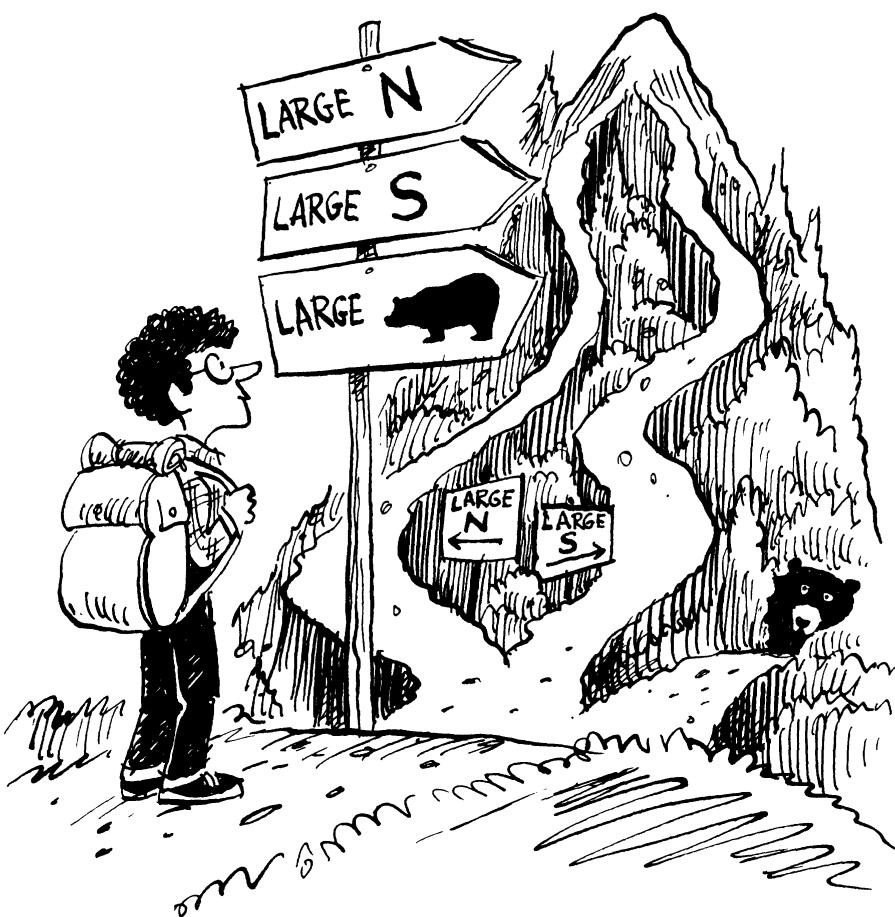
\includegraphics[width=0.5\textwidth]{deco_part3.jpg}

{\kaishu 插图：Dick Codor}
\end{center}

% 第10章 自旋路径积分
\chapter{自旋路径积分}

定义何谓“理解”一个特定体系总是困难的。即使拥有基态波函数与能量的精确解析形式，也未必能解释其物理性质。例如 $S = \frac{1}{2}$ Heisenberg 模型的 Bethe 拟设波函数，其关联仍需数值计算。理解一个模型有时意味着对其性质有一个简单的近似。一个近似——尽管不精确，甚至带有数学上的含糊——可能比精确解更有启发性。特别是，近似可以统一一族模型，并处理参数空间中精确可解点附近的一个开邻域。

路径积分提供形式表达式，由此引出有用的近似方案。通常它们无法以封闭解析形式求值\footnote{用 A. M. Polyakov 的话说：“路径积分没有现成的表可查。”}。尽管有这些缺点，它们仍是有价值的理论物理工具。凭借紧凑的表达式与记号，路径积分常用于生成渐近展开和表述平均场理论。

自旋相干态路径积分用单位矢量的时间历程描述量子自旋。这一图像高度直观，因为它把经典描述与量子现象联系起来。因此它是半经典近似的自然出发点，后者将在第 11、12、19 章描述。

\section{路径积分的构造}

自旋相干态可用于构造 Heisenberg 模型的路径积分表示。虚时表述中的生成泛函为\footnote{见附录 B 的 (B.17)。}

\begin{align*}
Z [ j ] & = \mathrm{Tr} \, T _ {\tau} \left( \exp \left[ - \int_ {0} ^ {\beta} d \tau \, \mathcal {H} ( \tau ) \right] \right)\\
& = \lim _ {N _ {\epsilon} \to \infty} \mathrm{Tr} \, T _ {\tau} \prod_ {n = 0} ^ {N _ {\epsilon} - 1} \left[ 1 - \epsilon \, \mathcal {H} ( \tau _ {n} ) \right] ,
\tag{10.1}
\end{align*}

其中 $\beta$ 是逆温度，$T_{\tau}$ 是时序算符，$\epsilon = \beta/N_{\epsilon}$ 是时间步长，$\tau_{n} = n\epsilon$ 是离散虚时间。生成哈密顿量含源流：

\begin{equation*}
\mathcal {H} ( \tau ) = \mathcal {H} - \sum_ {i \alpha} j _ {i} ^ {\alpha} ( \tau ) S _ {i} ^ {\alpha} \, , \quad \tau \in [ 0, \beta ) .
\tag{10.2}
\end{equation*}

构造路径积分的基本要素是 (7.25) 给出的单位分解。利用 (7.27)，在 (10.1) 的各因子之间插入 $N_{\epsilon}-1$ 次单位分解，得到多维积分

\begin{equation*}
Z [ j ] = \lim _ {N _ {\epsilon} \rightarrow \infty} \int \left( \prod_{\tau, i} d \hat {\Omega} _ {i \tau} \right) \prod_{\tau = \epsilon} ^ {\beta} \langle \hat {\Omega} ( \tau ) | \hat {\Omega} ( \tau - \epsilon ) \rangle \left[ 1 - \epsilon H ( \tau ) \right]
\tag{10.3}
\end{equation*}

其中 $\hat{\Omega} = (\hat{\Omega}_1, \ldots, \hat{\Omega}_{\mathcal{N}})$，“经典哈密顿量”定义为

\begin{equation*}
H ( \tau ) \equiv \frac {\langle \hat {\Omega} ( \tau ) | \mathcal {H} ( \tau ) | \hat {\Omega} ( \tau - \epsilon ) \rangle}{\langle \hat {\Omega} ( \tau ) | \hat {\Omega} ( \tau - \epsilon ) \rangle}.
\tag{10.4}
\end{equation*}

定义

\begin{equation*}
\hat {\Omega} ( \beta ) = \hat {\Omega} ( 0 )
\tag{10.5}
\end{equation*}

并注意测度对这两个时刻只算一次积分。

先验地，$\hat{\Omega}(\tau)$ 是 $\tau$ 的任意离散函数。下面我们将做一件明目张胆的非法操作：在 $N_{\epsilon} \to \infty$ 极限下把它当作连续可微函数，用导数代替差分：

\begin{equation*}
\frac {\hat {\Omega} _ {i} ( \tau + \epsilon ) - \hat {\Omega} _ {i} ( \tau )}{\epsilon} \Rightarrow \dot {\hat {\Omega}} _ {i} ( \tau ) + \mathcal {O} ( \epsilon ).
\tag{10.6}
\end{equation*}

(10.6) 的隐含假设是 $Z$ 由光滑路径主导，即 $|\dot{\Omega}| < \infty$。事实证明这一假设并不成立\footnote{见 Klauder，及 Schulman 书中第 31 章。}。忽略不连续路径，我们丢失了量子哈密顿量中算符排序的信息。尽管如此，我们仍将按可微函数的规则去操作“时间导数”。必须牢记我们的数学基础并不牢固；因此，凡是可能，都应当用不存在排序含糊的算符方法检验路径积分的结果。

利用 (7.19)，把相邻时间步的相干态交叠写出并展开到 $\epsilon$ 的领头阶：

\begin{equation*}
\langle \hat {\Omega} ( \tau + \epsilon ) | \hat {\Omega} ( \tau ) \rangle = \exp \left( - i S \epsilon \sum_ {i} \left( \dot {\phi} _ {i} \cos [ \theta_ {i} ( \tau ) ] + \dot {\chi} _ {i} \right) \right) ,
\tag{10.7}
\end{equation*}

其中 $\chi(\tau)$ 是任意规范约定。经典哈密顿量 (10.4) 乘以 $\epsilon$，可在等时计算：

\begin{equation*}
H [ \hat {\Omega} ( \tau ) ] \rightarrow \langle \hat {\Omega} ( \tau ) | \mathcal {H} ( \tau ) | \hat {\Omega} ( \tau ) \rangle .
\tag{10.8}
\end{equation*}

极限 $N_{\epsilon} \rightarrow \infty$ 把 (10.3) 变成路径积分。路径积分测度定义为

\begin{equation*}
\mathcal {D} \hat {\Omega} ( \tau ) = \lim _ {N _ {\epsilon} \rightarrow \infty} \prod_ {i, n} d \hat {\Omega} _ {i} ( \tau _ {n} ).
\tag{10.9}
\end{equation*}

对哈密顿量取指数、丢弃 $\epsilon$ 的高阶项，取 (10.3) 的形式连续极限，写为

\begin{align*}
Z [ j ] & = \oint \mathcal {D} \hat {\Omega} ( \tau ) \, \exp \left( - \tilde {\mathcal {S}} [ \hat {\Omega} ] \right) ,\\
\tilde {\mathcal {S}} [ \hat {\Omega} ] & = - i S \sum_ {i} \omega [ \hat {\Omega} _ {i} ] + \int_ {0} ^ {\beta} d \tau \, H [ \hat {\Omega} ( \tau ) ] .
\tag{10.10}
\end{align*}

记号 $\oint$ 反映周期边条件 (10.5)。对规范约定 $\chi_{i}(\tau)=0$，泛函 $\omega$ 依赖单个自旋的历程如下：

\begin{align*}
\omega [ \hat {\Omega} ] & = - \int_ {0} ^ {\beta} d \tau \, \dot {\phi} \cos \theta\\
& = - \int_ {\phi_ {0}} ^ {\phi_ {0}} d \phi \, \cos ( \theta_ {\phi} ) .
\tag{10.11}
\end{align*}

我们看到 $\omega$ 是几何的：它只依赖 $\hat{\Omega}_{i}(\tau)$ 在球面上的轨迹，而不依赖其显式时间依赖。泛函 $S\omega$ 也称为自旋历程的 Berry 相位，因为它描述与 $\hat{\Omega}(\tau)$ 平行的外磁场\footnote{见习题及 Shapere 与 Wilczek。}绝热转动时自旋所获得的相位。

现在将看到，Berry 相位度量路径 $\hat{\Omega}(\tau)$ 在单位球上围出的面积。路径增量 $d\hat{\Omega}$（如图~\ref{fig:10.1} 所示）通过经线 $\phi$ 与 $\phi + d\phi$ 连到北极。这个面积增量是球面上的一个三角形，其面积为

\begin{equation*}
d \omega ' = ( 1 - \cos \theta ) \, d \phi .
\tag{10.12}
\end{equation*}

于是由 $\theta (\tau), \phi (\tau)$ 参数化的闭合轨道围出的面积为

\begin{equation*}
\omega ' = \int_ {0} ^ {\beta} d \tau \, \dot {\phi} \left[ 1 - \cos \theta ( \tau ) \right].
\tag{10.13}
\end{equation*}

\begin{figure}[H]
\centering
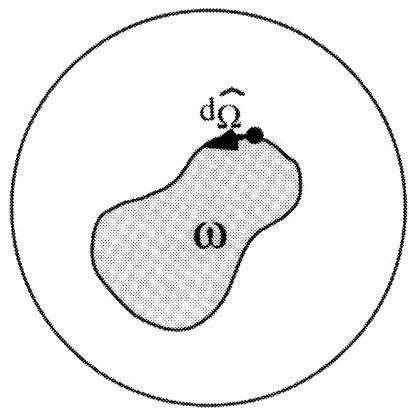
\includegraphics[width=0.5\textwidth]{fig10_1.jpg}
\caption{作为单位球上轨道的自旋历程。}
\label{fig:10.1}
\end{figure}

因此 $\omega'$ 是逆时针轨道 $\{\hat{\Omega} (\tau)\}_{0}^{\beta}$ 左侧围出的面积。恒等式

\begin{equation*}
\omega ' = \omega
\tag{10.14}
\end{equation*}

在 $\phi(\beta)$ 不越过“日界线”边界 $\pm\pi$ 时成立——这正是约定 (7.17) 的要求\footnote{$\omega$ 与 $\omega'$ 差别的澄清见习题 2。}。

把 Berry 相位 $\omega$ 写成规范不变的形式是有用的，即不指定球面的任何参数化（如 $\theta,\phi$）。引入矢量势 $\mathbf{A}(\hat{\Omega})$，满足

\begin{equation*}
\omega = \int_ {0} ^ {\beta} d \tau \, \mathbf {A} ( \hat {\Omega} ) \dot {\hat {\Omega}}.
\tag{10.15}
\end{equation*}

$\mathbf{A}(\hat{\Omega})$ 是单位磁单极矢量势，它沿轨道 $\{\hat{\Omega}(\tau)\}$ 的线积分等于该轨道张开的立体角 $\omega$。由 Stokes 定理，$\mathbf{A}$ 满足

\begin{equation*}
\nabla \times \mathbf {A} \cdot \hat {\Omega} = \epsilon^ {\alpha \beta \gamma} \frac {\partial A ^ {\beta}}{\partial \hat {\Omega} ^ {\alpha}} \hat {\Omega} ^ {\gamma} = 1 ,
\tag{10.16}
\end{equation*}

其中 $\epsilon^{\alpha\beta\gamma}$ 是全反对称张量，$\alpha,\beta,\gamma\in\{x,y,z\}$，重复指标求和。$\mathbf{A}$ 的两个标准选择是

\begin{align*}
\mathbf {A} ^ {a} & = - \frac {\cos \theta}{\sin \theta} \, \hat {\phi} ,\\
\mathbf {A} ^ {b} & = \frac {1 - \cos \theta}{\sin \theta} \, \hat {\phi}
\tag{10.17}
\end{align*}

\begin{equation*}
= \frac {\hat {z} \times \hat {\Omega}}{\hat {z} \cdot \hat {\Omega} + 1}.
\tag{10.18}
\end{equation*}

规范 $A^{b}$ 与 $A^{a}$ 的差别在于奇点的位置。$A^{a}$ 在北、南两极奇异；$\phi$ 的定义域是 $[-\pi, \pi)$，因而不允许越过 $\phi = \pm\pi$ 日界线的路径。反之，$A^{b}$ 只在南极 $\hat{\Omega} = -\hat{z}$ 有一个奇点——这正是携带磁单极通量的“Dirac 弦”进入球面的地方。对绕南极的无穷小轨道，$S\omega$ 的值为 $4\pi S$。由于 $S$ 是半整数，$\exp[-iS\omega]$ 是轨道的连续泛函，即使轨道越过规范场在南极的奇点。

\subsection{Green 函数}

Green 函数 $G(t)$ 描述零温的实时演化。它由演化算符在两个相干态之间的矩阵元给出：

\begin{equation*}
G ( \hat {\Omega} _ {0}, \hat {\Omega} _ {t}; t ) = \left\langle \hat {\Omega} _ {t} \left| T _ {t '} \left( \exp \left[ - i \int_ {0} ^ {t} d t ' \, \mathcal {H} ( t ' ) \right] \right) \right| \hat {\Omega} _ {0} \right\rangle ,
\tag{10.19}
\end{equation*}

其中 $T_{t'}$ 是实时排序算符（见 B.3）。$G(t)$ 可以用与 $Z$ 的路径积分极为类似的方式表示。在 (10.1)--(10.10) 的推导中，把虚时变量 $\tau$ 换成实时 $t'$：

\begin{equation*}
\begin{array}{ccc}
\tau & \to & i t '\\
t ' & \in & [ 0, t ]
\end{array}
\tag{10.20}
\end{equation*}

并把区间 $[0,t]$ 离散成 $N_{\epsilon}$ 个宽 $\epsilon$ 的步长。在 $(1-i\epsilon\mathcal{H})$ 各因子之间插入单位分解并取连续极限 $N_{\epsilon}\to\infty$（这将引入前述时间导数带来的数学含糊），得到形式表达式

\begin{equation*}
G ( t ) = \int_{\hat {\Omega} _ {0}} ^ {\hat {\Omega} _ {t}} \mathcal {D} \hat {\Omega} ( t ' ) \, \exp \left[ i \mathcal {S} [ \hat {\Omega} ] \right] ,
\tag{10.21}
\end{equation*}

其中 $\mathcal{S}$ 是实时作用量

\begin{equation*}
\mathcal {S} [ \hat {\Omega} ] = \int_ {0} ^ {t} d t ' \left( S \sum_ {i} \mathbf {A} \cdot \dot {\hat {\Omega}} - H [ \hat {\Omega} ( t ' ), t ' ] \right).
\tag{10.22}
\end{equation*}

\section{大 $S$ 展开}

自旋相干态路径积分 (10.10) 与 (10.21) 是导出半经典近似的方便出发点。坐标是单位矢量，即经典自旋；量子效应通过其（实或虚）时间依赖进入。我们可以把 $H[\hat{\Omega}]$ 的参数标度成与 $S$ 无关，即使用相应的经典哈密顿量 $H^{cl}[\hat{\Omega}]$\footnote{例如见 (6.35) 与 (6.36)。}。于是令 $S \to \infty$，一切 $\dot{\hat{\Omega}} \neq 0$ 的含时路径都被 Berry 相位因子的快速振荡压低，经典配分函数得以恢复：

\begin{equation*}
\lim _ {S \to \infty} Z [ j ] \sim Z ' \int \mathcal {D} \hat {\Omega} \, \exp \left[ - \beta H ^ {cl} [ \hat {\Omega} ] \right] ,
\tag{10.23}
\end{equation*}

其中 $Z'$ 包含归一化因子与高阶量子修正。右端积分就是经典哈密顿量 $H$ 的生成泛函。

也可以用 $S$ 作为控制参数，对 Green 函数作系统的渐近展开。这一半经典展开把量子修正引入经典理论。第一步是重标时间变量

\begin{align*}
\tau & \rightarrow S ^ {- 1} \tau = \bar {\tau} ,\\
\beta & \rightarrow S ^ {- 1} \beta = \bar {\beta} .
\tag{10.24}
\end{align*}

经典逆温度 $\bar{\beta}$ 取为与 $S$ 无关。这使我们可以把 $S$ 从作用量中标度出来：

\begin{align*}
Z ( \bar {\beta} ) & = \oint \mathcal {D} \hat {\Omega} ( \bar {\tau} ) \, \exp \left( - S \mathcal {S} ^ {cl} [ \hat {\Omega} ( \bar {\tau} ), \bar {\beta} ] \right) ,\\
\mathcal {S} ^ {cl} & = \int_ {0} ^ {\bar {\beta}} d \bar {\tau} \left( i \sum_ {i} \mathbf {A} \cdot \dot {\bar {\Omega}} - H ^ {cl} [ \hat {\Omega} ( \bar {\tau} ) ] \right) .
\tag{10.25}
\end{align*}

现在可以以 $S$ 为大参数，对 $Z$ 应用最陡下降法（见附录 E），得到对鞍点 $\hat{\Omega}^{cl,\alpha}$ 的求和（见 (E.14)）：

\begin{equation*}
Z \sim \sum_ {\alpha} \exp \left( - S \mathcal {S} ^ {cl} [ \hat {\Omega} ^ {cl, \alpha}, \bar {\beta} ] \right) Z _ {\alpha} ' ,
\tag{10.26}
\end{equation*}

鞍点方程为

\begin{equation*}
\left. \frac {\delta \mathcal {S} ^ {cl}}{\delta \hat {\Omega}} \right| _ {\hat {\Omega} = \hat {\Omega} ^ {cl, \alpha}} = 0.
\tag{10.27}
\end{equation*}

前置因子 $Z_{\alpha}'$ 含 $S^{-1}$ 幂次的次主导修正，可由展开涨落积分求得：

\begin{equation*}
Z _ {\alpha} ' = \oint \mathcal {D} \delta \hat {\Omega} \, \exp \left[ - S \left( \mathcal {S} ^ {cl} [ \hat {\Omega} ] - \mathcal {S} ^ {cl} [ \hat {\Omega} ^ {cl, \alpha} ] \right) \right] ,
\tag{10.28}
\end{equation*}

其中 $\delta \hat{\Omega} = \hat{\Omega} - \hat{\Omega}^{cl,\alpha}$。

\subsection{半经典动力学}

Green 函数的大 $S$ 展开要求标度

\begin{equation*}
t \rightarrow S t = \bar {t} ,
\tag{10.29}
\end{equation*}

这给出

\begin{align*}
G ( \bar {t} ) & = \int_{\hat {\Omega} _ {0}} ^ {\hat {\Omega} _ {\bar {t}}} \mathcal {D} \hat {\Omega} ( \bar {t} ' ) \, \exp \left( i S \mathcal {S} ^ {cl} [ \hat {\Omega} ] \right) ,\\
\mathcal {S} ^ {cl} & = \int_ {0} ^ {\bar {t}} d \bar {t} ' \left( \sum_ {i} \mathbf {A} \cdot \dot {\hat {\Omega}} - H ^ {cl} [ \hat {\Omega} ( \bar {t} ' ) ] \right) .
\tag{10.30}
\end{align*}

$G(t)$ 由使作用量取极值的含时路径 $\hat{\Omega}_{cl}(t')$ 主导。以下我们把 $\bar{t}$ 重记为 $t$。最陡下降法给出鞍点之和（见 (E.14)）：

\begin{equation*}
G \sim \sum_ {\alpha} \exp \left( i S \mathcal {S} [ \hat {\Omega} ^ {cl, \alpha}, \bar {t} ] \right) G _ {\alpha} ' ,
\tag{10.31}
\end{equation*}

$\hat{\Omega}^{cl}(t')$ 由鞍点方程

\begin{equation*}
\left. \frac {\delta}{\delta \hat {\Omega}} \mathcal {S} [ \hat {\Omega} ] \right| _ {\hat {\Omega} ^ {cl, \alpha}} = 0 ,
\tag{10.32}
\end{equation*}

以及边条件

\begin{align*}
\hat {\Omega} ^ {cl, \alpha} ( 0 ) & = \hat {\Omega} _ {0} ,\\
\hat {\Omega} ^ {cl, \alpha} ( t ) & = \hat {\Omega} _ {t}
\tag{10.33}
\end{align*}

确定。

作用量中 Berry 相位部分的变分为

\begin{align*}
\delta \omega [ \hat {\Omega} ] & = \int_ {0} ^ {t} d t ' \; \delta \left( \mathbf {A} \cdot \dot {\hat {\Omega}} \right)\\
& = \int_ {0} ^ {t} d t ' \left[ \frac {\partial A ^ {\alpha}}{\partial \hat {\Omega} ^ {\beta}} \delta \hat {\Omega} ^ {\beta} \dot {\hat {\Omega}} ^ {\alpha} + A ^ {\alpha} \frac {d}{d t} \delta \hat {\Omega} ^ {\alpha} \right]\\
& \quad + \left[ \frac {\partial A ^ {\alpha}}{\partial \hat {\Omega} ^ {\beta}} \dot {\hat {\Omega}} ^ {\beta} \delta \hat {\Omega} ^ {\alpha} - \frac {\partial A ^ {\alpha}}{\partial \hat {\Omega} ^ {\beta}} \dot {\hat {\Omega}} ^ {\beta} \delta \hat {\Omega} ^ {\alpha} \right]\\
& = \int_ {0} ^ {t} d t ' \, \frac {\partial A ^ {\alpha}}{\partial \hat {\Omega} ^ {\beta}} \epsilon^ {\alpha \beta \gamma} ( \dot {\hat {\Omega}} \times \delta \hat {\Omega} ) _ {\gamma} + \int_ {0} ^ {t} d t ' \, \frac {d}{d t '} \left( \mathbf {A} \cdot \delta \hat {\Omega} \right)\\
& = \int_ {0} ^ {t} d t ' \; \hat {\Omega} \cdot ( \dot {\hat {\Omega}} \times \delta \hat {\Omega} ) .
\tag{10.34}
\end{align*}

全导数的积分为零，因为端点被 (10.33) 固定。(10.34) 中还用了 (10.16) 与 $\hat{\Omega}$ 长度不变：

\begin{align*}
\delta \hat {\Omega} \cdot \hat {\Omega} & = \dot {\hat {\Omega}} \cdot \hat {\Omega} = 0 ,\\
\dot {\hat {\Omega}} \times \delta \hat {\Omega} & \parallel \hat {\Omega} ,
\tag{10.35}
\end{align*}

把 (10.34) 用于 (10.32)，得到经典 Euler--Lagrange 运动方程

\begin{align*}
\hat {\Omega} ^ {cl} \times \dot {\hat {\Omega}} ^ {cl} & = \frac {\partial H [ \hat {\Omega} ^ {cl} ]}{\partial \hat {\Omega}}\\
\Rightarrow \quad \dot {\hat {\Omega}} _ {i} ^ {cl} ( t ' ) & = \left. \hat {\Omega} ^ {cl} ( t ' ) \times \frac {\partial H}{\partial \hat {\Omega} _ {i} ( t ' )} \right| _ {\hat {\Omega} ^ {cl}} .
\tag{10.36}
\end{align*}

方程 (10.36) 描述“快速陀螺”极限下的经典转子系统，即转子内部转动能远大于转子间典型相互作用能的情形。第二行右端是作用在转子 $\hat{\Omega}_{i}$ 上的力矩，它改变方向但不改变大小\footnote{转子的经典力学见 Goldstein 的书。}。

利用 (10.36) 可以验证哈密顿量在经典路径上是运动常数：

\begin{align*}
\frac {d}{d t} H [ \hat {\Omega} ^ {cl} ( t ' ) ] & = \sum_ {i} \frac {\partial H}{\partial \hat {\Omega} _ {i} ( t ' )} \cdot \dot {\hat {\Omega}} _ {i} ^ {cl} ( t ' )\\
& = \sum_ {i} \frac {\partial H}{\partial \hat {\Omega} _ {i} ( t ' )} \cdot \left[ \hat {\Omega} _ {i} ^ {cl} ( t ' ) \times \frac {\partial H}{\partial \hat {\Omega} _ {i} ( t ' )} \right]\\
& = 0 ,
\tag{10.37}
\end{align*}

这保证能量沿经典轨迹守恒：$H[\hat{\Omega}^{cl}(t)] = H[\hat{\Omega}_{0}]$。

至此我们遇到一个问题：运动方程 (10.36) 对时间是一阶的，但解必须同时满足 $t' = 0$ 与 $t' = t$ 的两个边条件 (10.33)。对几乎所有边条件（例如 $H[\hat{\Omega}_{t}] \neq H[\hat{\Omega}_{0}]$ 时）这是不可能的。Klauder 建议了一种克服办法：在经典运动方程中添入阶为 $\epsilon$ 的二阶瞬态项。这样就可以在固定边条件下解二阶方程、计算经典作用量，最后取 $\epsilon \to 0$ 极限。

\subsection{半经典能谱}

依赖能量的 Green 函数定义为

\begin{equation*}
G ( \hat {\Omega} _ {0}, \hat {\Omega} _ {t}; E ) = i \int_ {0} ^ {\infty} d t \, G ( \hat {\Omega} _ {0}, \hat {\Omega} _ {t}; t ) \, e ^ {i ( E + i 0 ^ {+} ) t}.
\tag{10.38}
\end{equation*}

谱函数 $\Gamma(E)$ 为

\begin{align*}
\Gamma ( E ) & = \int d \hat {\Omega} _ {0} \, G ( \hat {\Omega} _ {0}, \hat {\Omega} _ {0}; E )\\
& = \sum_ {\alpha} \frac {1}{E - E _ {\alpha} + i 0 ^ {+}} .
\tag{10.39}
\end{align*}

$\Gamma(E)$ 的极点就是哈密顿量的本征能量 $\{E_{\alpha}\}$。

这里我们以非常粗略的方式，用经典周期轨道导出 $E_{\alpha}$ 的领头阶半经典近似。用路径积分导出半经典能谱的首创工作是 Gutzwiller；他的公式被广泛用于量子化具有混沌经典动力学的哈密顿量\footnote{这是一个称为“量子混沌”的研究领域，见文献注释。}。

$\Gamma(E)$ 的路径积分表示多了 $d\hat{\Omega}_{0}$ 与 $dt$ 积分。$\Gamma(E)$ 的半经典近似由 Gutzwiller 导出。经典路径的持续时间为 $t^{E}$，由 $dt$ 积分的鞍点近似确定：

\begin{equation*}
\left. \frac {\partial \mathcal {S} [ \hat {\Omega} ^ {cl} ]}{\partial t} \right| _ {t = t ^ {E}} + E = 0.
\tag{10.40}
\end{equation*}

由于 Berry 相位项 $\omega$ 是几何的，它不依赖 $t^{E}$。于是

\begin{equation*}
H ^ {cl} [ \hat {\Omega} ^ {cl} ] = E
\tag{10.41}
\end{equation*}

且

\begin{equation*}
\mathcal {S} ^ {cl} ( t ^ {E} ) + E t ^ {E} = \sum_ {i} \omega [ \hat {\Omega} _ {i} ].
\tag{10.42}
\end{equation*}

考虑能量为 $E$ 的周期轨道 $\hat{\Omega}_{i}^{E,\alpha}$，走过一次。如习题所示，对 $\hat{\Omega}_{0}$ 求迹的鞍点方程蕴含 $\dot{\hat{\Omega}}(0)=\dot{\hat{\Omega}}(t^{E})$。因此 $\Gamma$ 由对 $\hat{\Omega}_{i}^{E,\alpha}$ 的所有重复求和给出：

\begin{align*}
\Gamma & \sim \sum_ {\alpha} \sum_ {n} \exp \left( i n S \sum_ {i} \omega [ \hat {\Omega} _ {i} ^ {E, \alpha} ] \right)\\
& = \sum_ {\alpha} \frac {\exp \left( i S \sum_ {i} \omega [ \hat {\Omega} _ {i} ^ {E, \alpha} ] \right)}{1 - \exp \left( i S \sum_ {i} \omega [ \hat {\Omega} _ {i} ^ {E, \alpha} ] \right)} .
\tag{10.43}
\end{align*}

比较 (10.39) 与 (10.43)。半经典谱可由 (10.43) 的极点得到，$E_{\alpha}$ 由 Bohr--Sommerfeld 量子化条件确定：

\begin{equation*}
\sum_ {i} \omega [ \hat {\Omega} _ {i} ^ {E, \alpha} ] = 2 n \pi / S \; \Rightarrow \; E _ {\alpha} ^ {sc}.
\tag{10.44}
\end{equation*}

我们引用如下定理：若两个函数有相同的极点与留数，则它们至多差一个常数。于是，对量级为一的能量 $E_{\alpha}^{sc}$（即 $n = \mathcal{O}(S)$），(10.44) 按下式逼近量子谱：

\begin{equation*}
E _ {\alpha} = E _ {\alpha} ^ {sc} + \mathcal {O} ( 1/S ).
\tag{10.45}
\end{equation*}

\begin{exercises}

\item 相干态定义 (7.15) 中取 Euler 规范约定 $\chi = 0$ 给出 Berry 相位的表达式 (10.11)。若取 $\chi = -\phi$，证明 $\omega$ 改由 (10.13) 给出。

\item（Patrick Lee 的问题）：$\phi$ 在 (7.17) 中定义为半开区间 $[- \pi, \pi)$ 内。证明：若允许轨道 $\hat{\Omega}(t)$ 越过“日界线”$\phi = -\pi$，则 $\omega$ 的两个表达式 (10.11) 与 (10.13) 相差 $2\pi$；对半奇整数 $S$ 这对应于整体因子 $\exp(2\pi S) = -1$。为解决这一困难，如下计算 (10.11) 中环绕日界线的线积分：在经度 $\phi = -\pi + \epsilon$ 处从 $\theta$ 走到北极，环绕北极，再从日界线另一侧 $\phi = -\pi - \epsilon$ 处下到 $\theta$。

\item 考虑缓变的磁相互作用

\begin{equation*}
H [ \hat {\Omega} ( \tau ), \tau ] = - h ( \tau ) \, \hat {\Omega} ( \tau ) \cdot \mathbf {S} ,
\tag{10.46}
\end{equation*}

其中 $\tau \in [0, \beta]$ 参数化场的轨迹。设对所有 $\tau$ 有 $h(\tau) > 0$，把非简并的绝热基态定义为 $\Psi_0(\tau)$。证明由

\begin{equation*}
S \omega = \lim _ {dh / d\tau \rightarrow 0} \int_ {0} ^ {\beta} d \tau \, \operatorname{Im} \left\langle \frac {d}{d \tau} \Psi_ {0} ( \tau ) \middle| \Psi_ {0} ( \tau ) \right\rangle ,
\tag{10.47}
\end{equation*}

定义的 Berry 相位等于表达式 (10.11)。

\end{exercises}

\begin{chapbib}
\item 自旋相干态路径积分综述见
  J. Klauder, Phys. Rev. D \textbf{19}, 2349 (1979)。
\item 推荐的路径积分与半经典近似教科书：
  L. S. Schulman, \textit{Techniques and Applications of Path Integration} (Wiley, 1981)。
\item 关于 Berry 相位及其在物理各领域的大量出现，见
  A. Shapere and F. Wilczek, \textit{Geometric Phases in Physics} (World Scientific, 1989)。
\item 转子的经典运动方程求解见
  H. Goldstein, \textit{Classical Mechanics} (Addison-Wesley, 1981), 第五章。
\item 量子能级的半经典近似导出于
  M. C. Gutzwiller, J. Math. Phys. \textbf{12}, 343 (1971)。
\item 该主题（含量子混沌应用）的新近综述：
  M. C. Gutzwiller, \textit{Chaos and Quantum Physics}, edited by M. J. Giannoni, A. Voros, and J. Zinn-Justin (North Holland, 1992)。
\end{chapbib}

% 第11章 自旋波理论
\chapter{自旋波理论}

第 10 章我们构造了自旋路径积分，并证明其大 $S$ 极限恢复经典自旋的热力学与动力学。这里我们专门讨论量子 Heisenberg 模型，导出低阶（谐波）自旋波理论。这一途径对长程有序相的处理在物理上很有吸引力，因为量子效应以绕经典基态的（实或虚）时间依赖涨落的形式进入。自旋波模式与色散由线性化的经典运动方程得到。在 $1/S$ 的最低阶，自旋波是独立的谐振子，可以半经典地量子化。这一途径的一大优点是：对任何具有复杂基态的受挫 Heisenberg 模型都可以如法炮制。稍后我们再专门讨论较简单的铁磁与反铁磁情形。

然而，路径积分因动能项中时间导数的连续定义 (10.6) 而带有算符排序的含糊性。我们将用 Holstein--Primakoff 玻色子重新导出自旋波理论（该玻色子“先前在 11.2 节引入”\footnote{原书如此；HP 玻色子实际引入于 7.1 节，11.2 节是再次使用。}）。这将解决基态能量量子修正中的含糊。

\section{自旋波：路径积分途径}

考虑量子 Heisenberg 哈密顿量

\begin{equation*}
\mathcal {H} = \frac {1}{2} \sum_ {i, j} J _ {ij} \, \mathbf {S} _ {i} \cdot \mathbf {S} _ {j}.
\tag{11.1}
\end{equation*}

利用 (7.34)（习题 2），$\mathcal{H}$ 在相干态 $|\hat{\Omega}\rangle$ 中的期望值为

\begin{equation*}
H [ \hat {\Omega} ] = \langle \hat {\Omega} | \mathcal {H} | \hat {\Omega} \rangle = \frac {S ^ {2}}{2} \sum_ {i, j} J _ {ij} \, \hat {\Omega} _ {i} \cdot \hat {\Omega} _ {j}.
\tag{11.2}
\end{equation*}

$H$ 的经典基态依赖耦合常数 $J_{ij}$ 的细节。由模型的 $O(3)$ 对称性，整体自旋转动产生一个连续的简并基态流形。某些模型由于阻挫还有额外的基态简并。阻挫指没有任何组态能同时极小化所有单键相互作用。与 $H$ 的对称性无关的简并通常会被热涨落与量子涨落解除（lift）\footnote{文献中称为“无序导致的有序”（order due to disorder），见文献注释。}。这里不讨论受挫情形。

\begin{figure}[H]
\centering
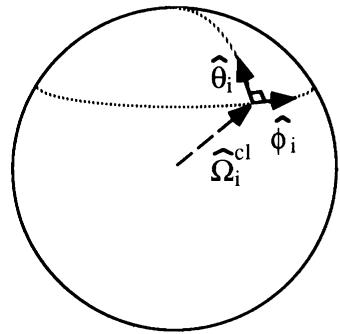
\includegraphics[width=0.48\textwidth]{fig11_1.jpg}
\caption{绕 $\hat{\Omega}^{cl}$ 的自旋涨落参数化。}
\label{fig:11.1}
\end{figure}

自旋波理论的基本假设是：可以选取经典基态流形中的一个成员 $\hat{\Omega}^{cl}$，以 10.2 节所述、由自旋大小 $S$ 控制的鞍点展开，把配分函数与 Green 函数绕它展开。

在每个格点取两个横向单位矢量 $\hat{\phi}_{i}, \hat{\theta}_{i}$，它们描述 $\hat{\Omega}_{i}^{cl}$ 处的方位角方向与经度方向，如图~\ref{fig:11.1}：

\begin{equation*}
\hat {\phi} _ {i} \times \hat {\theta} _ {i} = \hat {\Omega} _ {i} ^ {cl}.
\tag{11.3}
\end{equation*}

自旋涨落 $\delta\hat{\Omega} = \hat{\Omega} - \hat{\Omega}^{cl}$ 由两组投影变量参数化：

\begin{align*}
\mathbf {q} = \{ q _ {i} \} _ {1} ^ {\mathcal {N}} & \equiv \{ \delta \hat {\Omega} _ {i} \cdot \hat {\phi} _ {i} \} _ {1} ^ {\mathcal {N}} ,\\
\mathbf {p} = \{ p _ {i} \} _ {1} ^ {\mathcal {N}} & \equiv \{ S \, \delta \hat {\Omega} _ {i} \cdot \hat {\theta} _ {i} \} _ {1} ^ {\mathcal {N}} .
\tag{11.4}
\end{align*}

假设路径积分由小涨落主导，即 $|\delta\hat{\Omega}| \ll 1$。于是把测度换成相空间测度

\begin{equation*}
\mathcal {D} \delta \hat {\Omega} \rightarrow \nu \, \mathcal {D} \mathbf {q} \, \mathcal {D} \mathbf {p} \, , \quad \nu = \left( \frac {2 S + 1}{4 \pi S} \right) ^ {N _ {\epsilon} \mathcal {N}} ,
\tag{11.5}
\end{equation*}

$N_{\epsilon}$ 是时间步数，$\nu$ 是一个无穷大（但无趣）的归一化常数。$p$、$q$ 的积分域可扩为 $\int_{-\infty}^{\infty}$，得到相空间路径积分\footnote{实时相干态路径积分见 Schulman 的书。}：

\begin{equation*}
G \propto e ^ {i S [ \hat {\Omega} ^ {cl} ]} \int \mathcal {D} \mathbf {q} \, \mathcal {D} \mathbf {p} \, \exp \left[ \frac {i S}{2} \int_ {0} ^ {t} d t ' \, (\mathbf {q}, \mathbf {p}) \, \mathcal {L} ^ {(2)} \binom{\mathbf {q}}{\mathbf {p}} \right] \left[ 1 + \mathcal {O} (\mathbf {p}, \mathbf {q}) ^ {3} \right] ,
\tag{11.6}
\end{equation*}

其中 $\mathcal{L}^{(2)}$ 是绕固定基态组态 $\hat{\Omega}^{cl}$ 展开的自旋波 Lagrange 量矩阵。三次及更高阶涨落引入 $S^{-1}$ 更高阶的修正。由于 $\frac{d}{dt}\hat{\Omega}^{cl}=0$，Berry 相位的最低阶贡献为

\begin{align*}
S \sum_ {i} \omega_ {i} & \approx \frac {1}{2} S \sum_ {i} \int_ {0} ^ {t} d t ' \left( \hat {\Omega} ^ {cl} \cdot \delta \dot {\hat {\Omega}} \times \delta \hat {\Omega} \right)\\
& = \frac {1}{2} \int_ {0} ^ {t} d t ' \left( \mathbf {p} \cdot \dot {\mathbf {q}} - \dot {\mathbf {p}} \cdot \mathbf {q} \right),
\tag{11.7}
\end{align*}

这里用了 (10.34)。动能项 (11.7) 表明 $q$、$p$ 分别扮演坐标与正则动量的角色。

哈密顿量的二阶展开给出自旋波哈密顿量矩阵

\begin{align*}
H - H [ \hat {\Omega} ^ {cl} ] & \approx \frac {1}{2} (\mathbf {q}, \mathbf {p}) \, H ^ {(2)} \binom{\mathbf {q}}{\mathbf {p}} ,\\
H ^ {(2)} & = \left( \begin{array}{cc} K & P \\ P ^ {T} & M ^ {- 1} \end{array} \right) .
\tag{11.8}
\end{align*}

$H^{(2)}$ 是耦合谐振子的动力学矩阵，$M$、$K$ 分别是质量与力常数矩阵：

\begin{align*}
K & = \left. \frac {\partial^ {2} H}{\partial \mathbf {q} \, \partial \mathbf {q}} \right| _ {\mathbf {q} = \mathbf {p} = 0} ,\\
M ^ {- 1} & = \left. \frac {\partial^ {2} H}{\partial \mathbf {p} \, \partial \mathbf {p}} \right| _ {\mathbf {q} = \mathbf {p} = 0} .
\tag{11.9}
\end{align*}

$P$ 耦合坐标与动量：

\begin{equation*}
P = \left. \frac {\partial^ {2} H}{\partial \mathbf {p} \, \partial \mathbf {q}} \right| _ {\mathbf {q} = \mathbf {p} = 0}.
\tag{11.10}
\end{equation*}

组合 (11.7) 与 (11.8)，得到小振动对作用量的贡献

\begin{equation*}
\mathcal {S} ^ {(2)} \approx \mathcal {S} _ {0} + \int_ {0} ^ {t} d t ' \, (\mathbf {q}, \mathbf {p}) \, \mathcal {L} ^ {(2)} \binom{\mathbf {q}}{\mathbf {p}} ,
\tag{11.11}
\end{equation*}

其中

\begin{equation*}
L ^ {(2)} = - \left( \begin{array}{cc} K & \partial_ {t} + P \\ - \partial_ {t} + P ^ {T} & M ^ {- 1} \end{array} \right).
\tag{11.12}
\end{equation*}

自旋波模式 $(q_{\mathbf{k},\alpha}, p_{\mathbf{k},\alpha})$ 由解小振动的经典运动方程得到：

\begin{equation*}
\frac {\delta \mathcal {S} ^ {(2)} ( \mathbf {p}, \mathbf {q} )}{\delta \hat {\Omega}} = L ^ {(2)} \left( q _ {\mathbf {k}, \alpha} \; p _ {\mathbf {k}, \alpha} \right) \exp \left( i \omega_ {\mathbf {k}, \alpha} t \right) = 0.
\tag{11.13}
\end{equation*}

若 $\hat{\Omega}^{cl}$（从而 $L^{(2)}$）在格子上是周期的，自旋波以动量 $\mathbf{k}$ 与能带指标 $\alpha$ 标记。自旋波频率由特征方程

\begin{equation*}
\det \left( \begin{array}{cc} K & i \omega + P \\ - i \omega + P ^ {T} & M ^ {- 1} \end{array} \right)_{\omega = \omega_ {\mathbf {k}, \alpha}} = 0.
\tag{11.14}
\end{equation*}

给出。谐波自旋波是无相互作用的玻色子。其本征模式与能量使我们能计算所有热力学平均与动力学响应函数。特别地，自旋波对自由能的修正是

\begin{align*}
F ^ {(2)} & = \frac {T}{2} \ln \det \mathcal {L} ^ {(2)}\\
& = T \sum_ {\mathbf {k}, \alpha} \ln \sinh \left( \frac {\omega_ {\mathbf {k}}}{2 T} \right) .
\tag{11.15}
\end{align*}

可以把自旋波变换到 Bose 相干态变量（见附录 C）：

\begin{equation*}
\binom{\mathbf {z} _ {i} ( \tau )}{\mathbf {z} _ {i} ( \tau ) ^ {*}} = \frac {1}{\sqrt {2}} \left( \begin{array}{cc} 1 & i \\ 1 & - i \end{array} \right) \binom{\mathbf {q} _ {i} ( \tau )}{\mathbf {p} _ {i} ( \tau )}.
\tag{11.16}
\end{equation*}

$z$ 变量把相空间路径积分 (11.6) 变成 Bose 相干态路径积分\footnote{实时相干态路径积分见 Schulman 的书。}。测度之间满足

\begin{equation*}
\mathcal {D} \mathbf {p} \, \mathcal {D} \mathbf {q} = \mathcal {D} ^ {2} \mathbf {z}
\tag{11.17}
\end{equation*}

而动能项为

\begin{equation*}
\frac {i}{2} \int_ {0} ^ {t} d t ' \left( \mathbf {p} \cdot \dot {\mathbf {q}} - \dot {\mathbf {p}} \cdot \mathbf {q} \right) = \frac {1}{2} \int_ {0} ^ {t} d t ' \left( \mathbf {z} ^ {*} \dot {\mathbf {z}} - \dot {\mathbf {z}} ^ {*} \mathbf {z} \right).
\tag{11.18}
\end{equation*}

于是 Green 函数为

\begin{equation*}
G = \int \mathcal {D} ^ {2} \mathbf {z} \, \exp \left[ i \frac {1}{2} \int_ {0} ^ {t} d t ' \left( \mathbf {z} ^ {*} \dot {\mathbf {z}} - \dot {\mathbf {z}} ^ {*} \mathbf {z} \right) - H [ \mathbf {z} ^ {*}, \mathbf {z} ] \right] ,
\tag{11.19}
\end{equation*}

其中谐波 Bose 哈密顿量为

\begin{align*}
H [ \mathbf {z} ^ {*}, \mathbf {z} ] & \approx \frac {1}{2} ( \mathbf {z} ^ {*}, \mathbf {z} ) \, \tilde {H} ^ {(2)} \left( \begin{array}{l} \mathbf {z} \\ \mathbf {z} ^ {*} \end{array} \right) ,\\
\tilde {H} ^ {(2)} & = \left( \begin{array}{cc} \frac {1}{2} ( K + M ^ {- 1} ) & \frac {1}{2} ( K - M ^ {- 1} ) + iP \\ \frac {1}{2} ( K - M ^ {- 1} ) - iP & \frac {1}{2} ( K + M ^ {- 1} ) \end{array} \right)
\tag{11.20}
\end{align*}

同时含有正规（$z^{*}z$）与反常（$z^{*}z^{*}$ 及 $zz$）项。

用从实时间到虚时间的变换

\begin{equation*}
\begin{array}{ccc}
t ' & \rightarrow & - i \tau ,\\
t & \rightarrow & - i \beta .
\end{array}
\tag{11.21}
\end{equation*}

(11.19) 中 $G$ 的路径积分变成配分函数 (10.10)。自旋波对配分函数（定义见 (10.23)）的贡献为

\begin{align*}
Z ' & \approx \oint \mathcal {D} ^ {2} z \, \exp \left\{ - \beta \sum_ {\omega_ {n}} \left[ i \omega_ {n} \mathbf {z} ^ {*} \mathbf {z} - \frac {1}{2} ( \mathbf {z} ^ {*}, \mathbf {z} ) \tilde {H} ^ {(2)} \binom {\mathbf {z}} {\mathbf {z} ^ {*}} \right] \right\}\\
& = \prod_ {n} \det \left[ \left( \begin{array}{cc} i \omega_ {n} & 0 \\ 0 & - i \omega_ {n} \end{array} \right) - \tilde {H} ^ {(2)} \right] ^ {- 1}\\
\omega_ {n} & = 2 n \pi / \beta .
\tag{11.22}
\end{align*}

$\omega_{n}$ 是 Bose Matsubara 频率，$\sum_{\omega}$ 是附录 D（D.3 节）定义的离散 Matsubara 求和。

从相干态哈密顿量 (11.20) 反推二次量子化的 Bose 哈密顿量，得到

\begin{equation*}
\mathcal {H} ^ {(2)} = \frac {1}{2} \left( b ^ {\dagger}, b \right) \left( \begin{array}{cc} \frac {1}{2} ( K + M ^ {- 1} ) & \frac {1}{2} ( K - M ^ {- 1} ) + iP \\ \frac {1}{2} ( K - M ^ {- 1} ) - iP & \frac {1}{2} ( K + M ^ {- 1} ) \end{array} \right) \binom{b}{b ^ {\dagger}} + E _ {0} ' ,
\tag{11.23}
\end{equation*}

它同时含正规与反常项。$E_{0}'$ 是未知常数：(11.22) 的作用量不含 $\mathcal{H}^{(2)}$ 中 $b$ 与 $b^{\dagger}$ 正确排序的信息，这正是 $E_{0}'$ 含糊性的来源。下一节我们将用 Holstein--Primakoff 玻色子解决这一含糊。

方程 (11.13) 或 (11.23) 是通用的：一旦指定 $\hat{\Omega}^{cl}$，它们就确定任何 Heisenberg 模型的自旋波模式。下面我们限于最简单的模型——一、二、三维立方格子上的 Heisenberg 铁磁体与反铁磁体：

\begin{align*}
H & = \pm | J | S ^ {2} \sum_{\langle ij \rangle} \hat {\Omega} _ {i} \cdot \hat {\Omega} _ {j}\\
& = J S ^ {2} \sum_{\langle ij \rangle} \left[ \cos \theta_ {i} \cos \theta_ {j} + \sin \theta_ {i} \sin \theta_ {j} \cos ( \phi_ {i} - \phi_ {j} ) \right] ,
\tag{11.24}
\end{align*}

$\langle ij\rangle$ 表示立方格子上的近邻键。这些哈密顿量的自旋波展开特别简单，因为其经典基态要么是均匀铁磁体，要么是 Néel 反铁磁体。

\subsection{铁磁体}

假设路径积分绕有序的经典基态展开是有效的，可以用小磁场或边条件把自旋极化到 $\hat{x}$ 方向：

\begin{equation*}
\hat {\Omega} ^ {cl} = \left( \theta^ {cl}, \phi^ {cl} \right) = ( \pi / 2, 0 ).
\tag{11.25}
\end{equation*}

涨落参数化为

\begin{align*}
q _ {i} & = \phi _ {i} ,\\
p _ {i} & = S \cos \theta_ {i} .
\tag{11.26}
\end{align*}

对小的

\begin{equation*}
| \cos \theta | \ll 1 \, , \quad | \phi_ {i} | \ll \pi
\tag{11.27}
\end{equation*}

展开铁磁（$-|J|$）哈密顿量 (11.24)，保留到二阶（谐波）：

\begin{equation*}
H \approx - \frac {\mathcal {N} z}{2} | J | S ^ {2} + \frac {1}{2} | J | S ^ {2} \sum_{\langle ij \rangle} \left[ \frac {\left( p _ {i} - p _ {j} \right) ^ {2}}{S ^ {2}} + \left( q _ {i} - q _ {j} \right) ^ {2} \right] + \dots ,
\tag{11.28}
\end{equation*}

$\mathcal{N}$ 是格点数，$z = 2d$ 是 $d$ 维配位数。由 (11.9) 与 (11.10) 得 $P = 0$ 且

\begin{align*}
M _ {ij} ^ {- 1} & = - z | J | \, \nabla_ {ij} ^ {2} ,\\
K _ {ij} & = - z | J | S ^ {2} \nabla_ {ij} ^ {2} ,
\tag{11.29}
\end{align*}

其中格子 Laplace 算符由矩阵

\begin{equation*}
\nabla_ {ij} ^ {2} = z ^ {- 1} \sum_ {\eta} \left( \delta_ {i + \eta, j} - \delta_ {i, j} \right).
\tag{11.30}
\end{equation*}

给出，$\eta$ 是近邻矢量。$\nabla^{2}$ 的本征值为

\begin{align*}
\nabla_ {\mathbf {k}} ^ {2} & = \mathcal {N} ^ {- 1} \sum_ {ij} e ^ {- \mathbf {k} \cdot ( \mathbf {x} _ {i} - \mathbf {x} _ {j} )} \nabla_ {ij} ^ {2}\\
& = z ^ {- 1} \sum_ {\eta} \left( e ^ {i \mathbf {k} \eta} - 1 \right) \equiv \gamma_ {\mathbf {k}} - 1 ,
\tag{11.31}
\end{align*}

这定义了“紧束缚”函数 $\gamma_{k}$。(11.29) 代入 (11.14)：

\begin{equation*}
\det \left( \begin{array}{cc} - z | J | S ^ {2} ( \gamma_ {\mathbf {k}} - 1 ) & i \omega_ {\mathbf {k}} \\ - i \omega_ {\mathbf {k}} & - z | J | ( \gamma_ {\mathbf {k}} - 1 ) \end{array} \right) = 0 ,
\tag{11.32}
\end{equation*}

\begin{figure}[H]
\centering
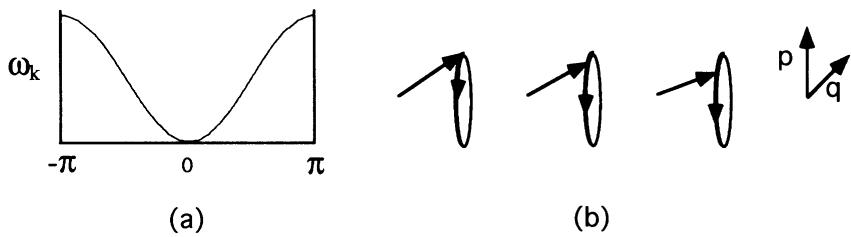
\includegraphics[width=0.55\textwidth]{fig11_2.jpg}
\caption{铁磁自旋波。(a)~$d = 1$ 的色散；(b)~$k \approx 0$ 的偏振。}
\label{fig:11.2}
\end{figure}

其零点在

\begin{equation*}
\omega_ {\mathbf {k}} \equiv z | J | S \left( 1 - \gamma_ {\mathbf {k}} \right).
\tag{11.33}
\end{equation*}

如习题 1 与图~\ref{fig:11.2} 所示，自旋波描述所有自旋绕 $\hat{x}$ 以角频率 $\omega_{k}$ 随时间进动。

\subsection{反铁磁体}

假设路径积分可以绕经典 Néel 态展开。不失一般性，取 Néel 态在子晶格 $A(B)$ 上指向 $\hat{x}(-\hat{x})$ 方向：

\begin{equation*}
\left( \theta_ {i} ^ {cl}, \phi_ {i} ^ {cl} \right) = \left\{ \begin{array}{ll} ( \pi / 2, 0 ) & i \in A \\ ( \pi / 2, - \pi ) & i \in B \end{array} \right. .
\tag{11.34}
\end{equation*}

（这里把矢量势的奇点定义在远离 $\hat{x}$ 与 $-\hat{x}$ 处是方便的，即用 (10.18) 的规范势，它只在南极奇异。）小涨落定义为

\begin{align*}
q _ {i} & = \left\{ \begin{array}{ll} \phi_ {i} & i \in A \\ \phi_ {i} + \pi & i \in B \end{array} \right. ,\\
p _ {i} & = S \cos \theta_ {i} .
\tag{11.35}
\end{align*}

反铁磁（$+|J|$）哈密顿量 (11.24) 的二阶展开为

\begin{equation*}
H \approx - \frac {\mathcal {N} z}{2} | J | S ^ {2} + \frac {1}{2} | J | S ^ {2} \sum_{\langle ij \rangle} \left[ \frac {\left( p _ {i} + p _ {j} \right) ^ {2}}{S ^ {2}} + \left( q _ {i} - q _ {j} \right) ^ {2} \right] + \dots .
\tag{11.36}
\end{equation*}

质量与力常数矩阵为

\begin{align*}
M _ {ij} ^ {- 1} & = z J \left( \nabla_ {ij} ^ {2} + \frac {2}{z} \delta_ {ij} \right) ,\\
K _ {ij} & = - z J S ^ {2} \nabla_ {ij} ^ {2} ,
\tag{11.37}
\end{align*}

\begin{figure}[H]
\centering
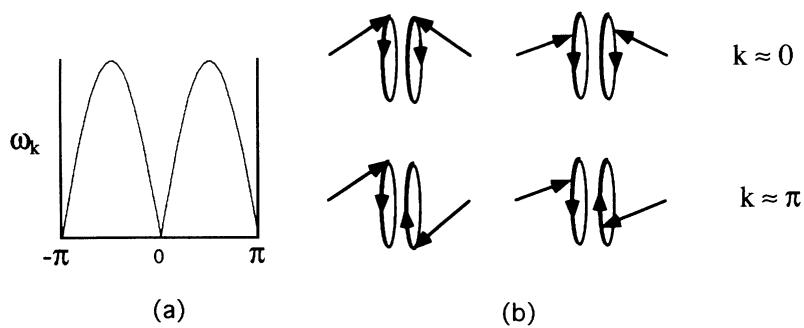
\includegraphics[width=0.55\textwidth]{fig11_3.jpg}
\caption{反铁磁自旋波。(a)~$d = 1$ 的色散；(b)~两个简并模式的偏振。}
\label{fig:11.3}
\end{figure}

可在 Fourier 空间中同时对角化为

\begin{align*}
M _ {\mathbf {k}} ^ {- 1} & = z J \left( 1 + \gamma_ {\mathbf {k}} \right) ,\\
K _ {\mathbf {k}} & = z J S ^ {2} \left( 1 - \gamma_ {\mathbf {k}} \right) .
\tag{11.38}
\end{align*}

解 (11.14) 得自旋波谱：

\begin{equation*}
\det \left( \begin{array}{cc} - z | J | S ^ {2} ( \gamma_ {\mathbf {k}} - 1 ) & i \omega_ {\mathbf {k}} \\ - i \omega_ {\mathbf {k}} & z | J | ( \gamma_ {\mathbf {k}} + 1 ) \end{array} \right) = 0 ,
\tag{11.39}
\end{equation*}

对立方格子给出两个模式

\begin{equation*}
\omega_ {\mathbf {k}} \equiv z J S \sqrt {1 - \gamma_ {\mathbf {k}} ^ {2}} \sim c \left| \mathbf {k} - \mathbf {k} _ {c} \right| ,
\tag{11.40}
\end{equation*}

其中 $\mathbf{k}_c = 0, \vec{\pi}$，$\vec{\pi} = (\pi, \pi, \ldots)$。$d$ 维立方格子的自旋波速度为

\begin{equation*}
c = 2 \sqrt {d} \, J S.
\tag{11.41}
\end{equation*}

反铁磁自旋波是绕经典方向 $\pm\hat{x}$ 进动的单位矢量。如习题 2 与图~\ref{fig:11.3} 所示，两个子晶格上的自旋沿相反方向进动。与铁磁自旋波 (11.33) 不同，存在两个简并的反铁磁自旋波模式，其频率分别在 $k\rightarrow0$ 与 $k\rightarrow\vec{\pi}$ 处消失。

\section{自旋波：Holstein--Primakoff 途径}

上一节我们看到低阶自旋波可以写成无相互作用的玻色子。作为定量的量子理论，必须确定哈密顿量中 Bose 算符的正确次序。

为此，用 Holstein--Primakoff（HP）玻色子表示量子模型。HP 玻色子此前在 (7.1) 中相对自旋空间的 $\hat{z}$ 方向定义。这里把定义推广到使 $H[\hat{\Omega}]$ 极小的任意经典组态 $\hat{\Omega}_{i}^{cl}$。用 $\hat{\Omega}^{cl}$ 可在每个格点定义三个基底矢量 $(\mathbf{e}^{1},\mathbf{e}^{2},\hat{\Omega}^{cl})$：

\begin{equation*}
\mathbf {e} _ {i} ^ {1} \times \mathbf {e} _ {i} ^ {2} = \hat {\Omega} _ {i} ^ {cl}.
\tag{11.42}
\end{equation*}

这一坐标系中的升降算符为

\begin{equation*}
S ^ {\pm} = \mathbf {S} \cdot \mathbf {e} ^ {1} \pm i \, \mathbf {S} \cdot \mathbf {e} ^ {2}.
\tag{11.43}
\end{equation*}

与 (7.1) 类似，自旋分量（相对 (11.42) 的三元组）可用 HP 玻色子表示：

\begin{align*}
S ^ {+} & = \left( \sqrt {2 S - n _ {b}} \, \right) b ,\\
S ^ {-} & = b ^ {\dagger} \sqrt {2 S - n _ {b}} ,\\
\mathbf {S} \cdot \hat {\Omega} ^ {cl} & = - n _ {b} + S .
\tag{11.44}
\end{align*}

这一表示在 $n_{b} \leq 2S$ 的 Hilbert 子空间中是精确的。然而平方根函数代表数算符乘以 $1/S$ 因子的无穷幂级数。若能事后证明

\begin{equation*}
\langle n _ {b} \rangle \ll 2 S ,
\tag{11.45}
\end{equation*}

即绕经典方向的自旋涨落很小，则级数截断到低阶就是合理的。

下一步，把哈密顿量中的自旋算符换成 (11.42) 型表达式，合并 $1/S$ 同阶的项。玻色子的二次阶以下各项构成自旋波哈密顿量。

\subsection{铁磁体}

不失一般性，取经典方向沿 $\hat{z}$，把 HP 算符代入铁磁哈密顿量：

\begin{align*}
\mathcal {H} & = - | J | \sum_{\langle ij \rangle} \mathbf {S} _ {i} \cdot \mathbf {S} _ {j}\\
& = - S ^ {2} | J | \mathcal {N} z / 2 - 2 | J | \sum_{\langle ij \rangle} \Big[ S b _ {i} ^ {\dagger} \sqrt {1 - n _ {i} / 2S} \sqrt {1 - n _ {j} / 2S} \, b _ {j}\\
& \quad - \frac {1}{2} S \left( n _ {i} + n _ {j} \right) + \frac {1}{2} n _ {i} n _ {j} \Big] .
\tag{11.46}
\end{align*}

用 (7.4) 展开平方根，收集到 $1/S^{0}$ 阶：

\begin{align*}
\mathcal {H} & \approx - S ^ {2} | J | \mathcal {N} z / 2 + H _ {1} + H _ {2} + \mathcal {O} ( 1/S ) ,\\
H _ {1} & = \sum_ {\mathbf {k}} \omega_ {\mathbf {k}} \, b _ {\mathbf {k}} ^ {\dagger} b _ {\mathbf {k}} ,\\
H _ {2} & = | J | / 4 \sum_{\langle ij \rangle} \left[ b _ {i} ^ {\dagger} b _ {j} ^ {\dagger} \left( b _ {i} - b _ {j} \right) ^ {2} + \left( b _ {i} ^ {\dagger} - b _ {j} ^ {\dagger} \right) ^ {2} b _ {i} b _ {j} \right] ,
\tag{11.47}
\end{align*}

其中

\begin{equation*}
b _ {\mathbf {k}} = \frac {1}{\sqrt {\mathcal {N}}} \sum_ {i} e ^ {- i \mathbf {k} \cdot \mathbf {x} _ {i}} b _ {i}
\tag{11.48}
\end{equation*}

而

\begin{equation*}
\omega_ {\mathbf {k}} = S | J | z \left( 1 - z ^ {- 1} \sum_{j \, \in \langle ij \rangle} e ^ {i ( \mathbf {x} _ {j} - \mathbf {x} _ {i} ) \mathbf {k}} \right) \equiv S | J | z \left( 1 - \gamma_ {\mathbf {k}} \right) ,
\tag{11.49}
\end{equation*}

与 (11.33) 一致。$H_{1}$ 描述色散为 $\omega_{k}$ 的无相互作用自旋波。$H_{2}$ 及更高阶项描述自旋波间的相互作用，可用微扰论或平均场近似处理。$T = 0$ 时，由 (11.47) 显然能量等于经典能量

\begin{equation*}
E _ {0} = - S ^ {2} | J | \mathcal {N} z / 2.
\tag{11.50}
\end{equation*}

这与第 5 章定理 5.1 相符：量子铁磁体的基态就是经典基态。

铁磁自旋波色散的长波极限按

\begin{equation*}
\omega_ {\mathbf {k}} \sim S | J | | \mathbf {k} | ^ {2}
\tag{11.51}
\end{equation*}

消失。这是无能隙的 Goldstone 模，是铁磁基态破缺对称的结果（见 9.2 节）。Goldstone 模主导铁磁体低温、长波关联。有限温下基态磁化的最低阶修正为

\begin{align*}
\Delta m _ {0} & = \frac {1}{\mathcal {N}} \langle S _ {\mathrm{tot}} ^ {z} \rangle - S\\
& = - \langle n _ {i} \rangle = - \frac {1}{\mathcal {N}} \sum_ {\mathbf {k}} n _ {\mathbf {k}} ,
\tag{11.52}
\end{align*}

其中 Bose--Einstein 占据数为（见 (A.25)）

\begin{equation*}
n _ {\mathbf {k}} = \frac {1}{e ^ {\omega_ {\mathbf {k}} / T} - 1}.
\tag{11.53}
\end{equation*}

(11.52) 中求和的低温渐近行为，可通过引入小的“红外”截断 $k_{0}$ 求得。再取一个位于 (11.51) 适用区内的小而有限的动量 $\bar{k} > k_{0}$，即

\begin{equation*}
\omega_ {\bar {k}} \ll T \ll | J | S.
\tag{11.54}
\end{equation*}

把 (11.52) 中的求和分成 $k_{0} < |k| < \bar{k}$ 与 $|k| \geq \bar{k}$ 两段：

\begin{equation*}
\Delta m _ {0} \approx - \int_{k _ {0}} ^ {\bar {k}} \frac {d k \, k ^ {d - 1}}{( 2 \pi ) ^ {d}} \frac {T}{J S k ^ {2}} - \mathcal {N} ^ {- 1} \sum_{| \mathbf {k} | > \bar {k}} \frac {1}{\exp [ \omega_ {\mathbf {k}} / T ] - 1}.
\tag{11.55}
\end{equation*}

$d = 1, 2$ 且 $T > 0$ 时，第一个积分在 $k_{0} \to 0$ 发散：

\begin{equation*}
\Delta m _ {0} \propto \left\{ \begin{array}{ll} - \dfrac {t}{k _ {0}} + \dots & d = 1 \\[4pt] t \log k _ {0} + \dots & d = 2 \end{array} \right. ,
\tag{11.56}
\end{equation*}

其中 $t = T/(JS)$。(11.55) 的第二个求和有限，不影响红外奇性。(11.56) 最重要的结论是：在一维、二维，涨落引起的磁化修正随红外截断 $k_{0}$ 消失而发散。因此我们最初的假设——自旋涨落 $\langle(S_{i}^{z} - S)^{2}\rangle$ 很小——在这些情形是不成立的，HP 展开的低阶截断不合法。自旋波理论的失效与 Mermin--Wagner 定理 6.2 一致：后者确实排除了 $d=1,2$ 在一切非零温度下的有限自发磁化。

$d = 3$ 没有红外发散。$M$ 的领头温度依赖可以这样计算：把 Bose 函数 (11.53) 写成几何级数，动量积分上限取到无穷：

\begin{align*}
\Delta m _ {0} ^ {d = 3} & = - \int_{k _ {0}} ^ {\bar {k}} \frac {d k \, k ^ {2}}{2 \pi^ {2}} \sum_ {n = 1} ^ {\infty} \exp [ - n k ^ {2} / t ] \left[ 1 + \mathcal {O} ( t ) \right]\\
& \approx - \frac {1}{8} \left( \frac {t}{\pi} \right) ^ {3/2} \sum_ {n = 1} ^ {\infty} n ^ {- 3/2} = - \frac {1}{8} \left( \frac {t}{\pi} \right) ^ {3/2} \zeta ( 3/2 ) ,
\tag{11.57}
\end{align*}

$\zeta$ 是 Riemann $\zeta$ 函数 $\zeta(s)=\sum_{n}n^{-s}$。于是三维中有序矩的领头温度修正正比于 $-T^{3/2}$。

\subsection{反铁磁体}

这里取经典 Néel 态沿子晶格 A、B 的 $\hat{z}$ 与 $-\hat{z}$ 方向。定义转动后的自旋 $\tilde{S}$（对 $j \in B$）：

\begin{align*}
j \in B :\quad \tilde {S} _ {j} ^ {z} & = - S _ {j} ^ {z} ,\\
\tilde {S} _ {j} ^ {x} & = S _ {j} ^ {x} ,\\
\tilde {S} _ {j} ^ {y} & = - S _ {j} ^ {y} .
\tag{11.58}
\end{align*}

显然 $\tilde{S}^{\alpha}$ 与 $S^{\alpha}$ 满足相同的对易关系，因此同样可用 Holstein--Primakoff 玻色子表示。用子晶格转动后的表示，反铁磁哈密顿量为

\begin{align*}
\mathcal {H} & = - | J | \sum_{\langle ij \rangle} S _ {i} ^ {z} \tilde {S} _ {j} ^ {z}\\
& \quad + \frac {1}{2} | J | \sum_{\langle ij \rangle} \left( S _ {i} ^ {+} \tilde {S} _ {j} ^ {+} + S _ {i} ^ {-} \tilde {S} _ {j} ^ {-} \right) .
\tag{11.59}
\end{align*}

对子晶格 $A$ 的 $\mathbf{S}$ 与子晶格 $B$ 的 $\tilde{\mathbf{S}}$ 用 HP 玻色子表示 (11.44)：

\begin{align*}
\mathcal {H} & = - S ^ {2} J \mathcal {N} z / 2 + \mathcal {H} _ {1} + \mathcal {H} _ {2} + \mathcal {O} ( 1/S ) ,\\
\mathcal {H} _ {1} & = J S z \sum_ {\mathbf {k}} \left[ b _ {\mathbf {k}} ^ {\dagger} b _ {\mathbf {k}} + \frac {\gamma_ {\mathbf {k}}}{2} \left( b _ {\mathbf {k}} ^ {\dagger} b _ {- \mathbf {k}} ^ {\dagger} + b _ {\mathbf {k}} b _ {- \mathbf {k}} \right) \right] ,\\
\mathcal {H} _ {2} & = - \frac {J}{4} \sum_{\langle ij \rangle} \left[ b _ {i} ^ {\dagger} \left( b _ {j} ^ {\dagger} + b _ {i} \right) ^ {2} b _ {j} + b _ {j} ^ {\dagger} \left( b _ {i} ^ {\dagger} + b _ {j} \right) ^ {2} b _ {i} \right] .
\tag{11.60}
\end{align*}

$\mathcal{H}_{1}$ 是含正规与反常项（如 $a^{\dagger}a^{\dagger}$）的二次哈密顿量，可用 Bogoliubov 变换对角化。定义自旋波算符 $\alpha_{\mathbf{k}}$：

\begin{align*}
\alpha_ {\mathbf {k}} & = \cosh \theta_ {\mathbf {k}} \, a _ {\mathbf {k}} - \sinh \theta_ {\mathbf {k}} \, a _ {- \mathbf {k}} ^ {\dagger} ,\\
a _ {\mathbf {k}} & = \cosh \theta_ {\mathbf {k}} \, \alpha_ {\mathbf {k}} + \sinh \theta_ {\mathbf {k}} \, \alpha_ {- \mathbf {k}} ^ {\dagger} .
\tag{11.61}
\end{align*}

参数 $\theta_{\mathbf{k}}$ 为实，且在 $\mathbf{k} \to -\mathbf{k}$ 下为偶。(11.61) 是正则变换，因为

\begin{align*}
\left[ \alpha_ {\mathbf {k}}, \alpha_ {\mathbf {k} '} ^ {\dagger} \right] & = \delta_ {\mathbf {kk} '} ,\\
\left[ \alpha_ {\mathbf {k}}, \alpha_ {\mathbf {k} '} \right] & = \left[ \alpha_ {\mathbf {k}} ^ {\dagger}, \alpha_ {\mathbf {k} '} ^ {\dagger} \right] = 0 .
\tag{11.62}
\end{align*}

用自旋波算符表示：

\begin{align*}
\mathcal {H} _ {1} & = | J | S z \sum_ {\mathbf {k}} \Big[ \left( \cosh 2 \theta_ {\mathbf {k}} + \gamma_ {\mathbf {k}} \sinh 2 \theta_ {\mathbf {k}} \right) \alpha_ {\mathbf {k}} ^ {\dagger} \alpha_ {\mathbf {k}}\\
& \quad + \frac {1}{2} \left( \sinh 2 \theta_ {\mathbf {k}} + \gamma_ {\mathbf {k}} \cosh 2 \theta_ {\mathbf {k}} \right) \left( \alpha_ {\mathbf {k}} ^ {\dagger} \alpha_ {- \mathbf {k}} ^ {\dagger} + \alpha_ {\mathbf {k}} \alpha_ {- \mathbf {k}} \right)\\
& \quad + \sinh^ {2} \theta_ {\mathbf {k}} + \frac {\gamma_ {\mathbf {k}}}{2} \sinh 2 \theta_ {\mathbf {k}} \Big] .
\tag{11.63}
\end{align*}

选 $\theta_{k}$ 使反常项 $\alpha^{\dagger}\alpha^{\dagger}$ 与 $\alpha\alpha$ 消失，条件是

\begin{equation*}
\tanh 2 \theta_ {\mathbf {k}} = - \gamma_ {\mathbf {k}} ,
\tag{11.64}
\end{equation*}

由此得

\begin{align*}
\mathcal {H} _ {1} & = \sum_ {\mathbf {k}} \omega_ {\mathbf {k}} \left( \alpha_ {\mathbf {k}} ^ {\dagger} \alpha_ {\mathbf {k}} + \frac {1}{2} \right) - \frac {J S z \mathcal {N}}{2} ,\\
\omega_ {\mathbf {k}} & = | J | S z \sqrt {1 - \gamma_ {\mathbf {k}} ^ {2}} ,
\tag{11.65}
\end{align*}

与 (11.40) 一致。由 (11.65) 可见，与铁磁体 (11.50) 不同，$H_{1}$ 含有大小为

\begin{equation*}
E _ {0} ' = E _ {0} - \left( - \frac {z}{2} \mathcal {N} | J | S ^ {2} \right) = \frac {1}{2} \sum_{\mathbf {k}} | J | S z \left( \sqrt {1 - \gamma_{\mathbf {k}} ^ {2}} - 1 \right).
\tag{11.66}
\end{equation*}

的量子零点能。注意 $E_{0}'$ 为负，即量子涨落降低反铁磁体的能量。考虑两格点的最简单情形即可理解：经典基态能量为 $-JS^{2}$，而量子能量明显更低：$-JS(S+1)$。

量子反铁磁体的基态是 $\alpha$ 玻色子的真空。Bogoliubov 变换使基态中混入任意数目的 HP 玻色子；用自旋语言说，基态混入了相对 Néel 态含任意数目自旋翻转的组态。这削弱 $T = 0$ 的长程 Néel 序。

在 $\mathbf{k} = 0$ 与 $\mathbf{k} = \vec{\pi} = (\pi, \pi, \ldots)$ 附近，自旋波谱按

\begin{equation*}
\omega_ {\mathbf {k}} \sim \left\{ \begin{array}{ll} J S \sqrt {2 z} \, | \mathbf {k} | & | \mathbf {k} | \approx 0 \\ J S \sqrt {2 z} \, | \mathbf {k} - ( \pi, \pi, \ldots ) | & \mathbf {k} \approx ( \pi, \pi, \ldots ) \end{array} \right.
\tag{11.67}
\end{equation*}

消失。序参量是交错磁化。其低阶修正由 $H_{1}$ 给出：

\begin{align*}
\Delta m _ {0} ^ {s} & = \frac {1}{\mathcal {N}} \Big\langle \sum_ {i} e ^ {i \vec {\pi} \mathbf {X} _ {i}} S _ {i} ^ {z} \Big\rangle - S\\
& = - \frac {1}{\mathcal {N}} \Big\langle \sum_ {i} a _ {i} ^ {\dagger} a _ {i} \Big\rangle\\
& = + \frac {1}{2} - \frac {1}{\mathcal {N}} \sum_ {\mathbf {k}} \left( n _ {\mathbf {k}} + \frac {1}{2} \right) \frac {1}{\sqrt {1 - \gamma_{\mathbf {k}} ^ {2}}} .
\tag{11.68}
\end{align*}

与铁磁体一样，只有当 $\Delta m_{0}^{s} \ll S$ 时，HP 展开截断到二次阶才是合理的。

低温下 $\Delta m_{0}^{s}$ 的领头红外奇性由展开 Bose 函数（在 $\omega_{k} \approx 0$ 附近）求得。用 $k_{0}$ 截断 $k \approx 0$ 与 $k \approx \vec{\pi}$ 附近的动量和：

\begin{equation*}
\Delta m _ {0} \sim \left\{ \begin{array}{ll} \dfrac {c _ {1}}{k _ {0}} & d = 1 \\[4pt] - c _ {2} + t \log k _ {0} & d = 2 \\[4pt] - c _ {3} + c _ {3} ' t ^ {2} & d = 3 \end{array} \right.
\tag{11.69}
\end{equation*}

其中

\begin{align*}
c _ {d} & = \frac {1}{2 \mathcal {N}} \sum_ {\mathbf {k}} \frac {1}{\sqrt {1 - \gamma_{\mathbf {k}} ^ {2}}} - 1 \, , \ d = 2, 3 ,\\
c _ {3} ' & = 6 ^ {- 5/2} / 2 ,\\
t & = \frac {T}{| J | S \sqrt {d}} .
\tag{11.70}
\end{align*}

与铁磁体情形一样，只有当存在真长程序且 $\Delta m_{0}^{s} \ll S$ 时，HP 展开的截断才是合理的。注意一维中交错磁化修正实际上随 $k_{0} \to 0$ 发散，这标志着自旋波理论的失败和基态无长程序。稍后我们将看到，$d$ 维量子模型基态长程序的缺失，与 $d+1$ 维经典 Heisenberg 模型有限温的 Mermin--Wagner 定理相关。

我们还注意到，由 (11.69)，$d = 2, 3$ 基态长程序的存在与否取决于 $c'$ 与 $S$ 的相对大小。$d=3$ 是有限温下可能存在长程自旋序的最低维数。

\begin{exercises}

\item 把 (11.13) 用于铁磁自旋波模式，证明 $k \approx 0$ 处进动自旋的方向如图~\ref{fig:11.2} 所示。

\item 对一维反铁磁体 $k = 0$ 与 $k = \pi$ 的两个自旋波模式重复上题，并与图~\ref{fig:11.3} 比较。

\item 近邻键的 Néel 矢量定义为

\begin{equation*}
\hat {\mathbf {n}} = \frac {1}{2} \left( \hat {\Omega} _ {i} - \hat {\Omega} _ {j} \right).
\tag{11.71}
\end{equation*}

证明 $\hat{n}$ 近似地作周期性平面振荡。求 $k = 0$ 与 $k = \vec{\pi}$ 时 $\hat{n}$ 的偏振面。

\item 考虑立方格子上的亚铁磁体：子晶格 A 上大小为 $S_{A}$ 的自旋与子晶格 B 上大小为 $S_{B}$ 的近邻自旋反铁磁耦合。循 11.1.2 小节，用自旋波理论计算元激发的色散。

\item 反铁磁自旋波哈密顿量 $\mathcal{H}_1$（见 (11.60)）的基态必须满足

\begin{equation*}
\alpha_ {\mathbf {k}} \Psi_ {0} = 0 \, , \quad \forall \mathbf {k}.
\tag{11.72}
\end{equation*}

用 (11.61) 中 $\alpha_{\mathbf{k}}$ 的定义证明

\begin{align*}
\Psi_ {0} & = \nu \exp \left[ \frac {1}{2} \sum_ {\mathbf {k}} u _ {\mathbf {k}} b _ {\mathbf {k}} ^ {\dagger} b _ {- \mathbf {k}} ^ {\dagger} \right] \left| 0 \right\rangle ,\\
u _ {\mathbf {k}} & = \tanh \theta_ {\mathbf {k}} .
\tag{11.73}
\end{align*}

求归一化常数 $\nu$。注意：(11.73) 的 $\Psi_{0}$ 不是纯自旋态，因为它含有 $n_{b} > 2S$ 非物理态的贡献。用自旋升降算符替换 HP 玻色子可以定义合适的变分自旋态。

\item 求 $u_{ij}$ 对大 $|x_{i}-x_{j}|$ 的渐近衰减：

\begin{equation*}
u _ {ij} = \frac {1}{\mathcal {N}} \sum_ {\mathbf {k}} u _ {\mathbf {k}} \exp \left[ - i \mathbf {k} \cdot ( \mathbf {x} _ {i} - \mathbf {x} _ {j} ) \right] ,
\tag{11.74}
\end{equation*}

其中 $u_{\mathbf{k}}$ 已在 (11.73) 定义。提示：用量纲分析把 $|\mathbf{x}_i - \mathbf{x}_j|$ 的幂次从积分中标度出来。

\item 用 HP 表示对铁磁体展开各向同性自旋关联函数

\begin{equation*}
S ( \mathbf {q} ) = \mathcal {N} ^ {- 1} \langle \mathbf {S}_{\mathbf {q}} \cdot \mathbf {S} _ {- \mathbf {q}} \rangle
\tag{11.75}
\end{equation*}

到四玻色子项。用成对收缩把有限温的 $S(\mathbf{q})$ 写成单个动量求和。

\end{exercises}

\begin{chapbib}
\item 自旋波理论的开创性工作：
  P. W. Anderson, Phys. Rev. \textbf{83}, 1260 (1951)；
  R. Kubo, Phys. Rev. \textbf{87}, 568 (1952)；
  T. Oguchi, Phys. Rev. \textbf{117}, 117 (1960)。
\item 自旋波理论及应用的大量综述见
  D. C. Mattis, \textit{Theory of Magnetism I} (Springer-Verlag, 1988)；
  R. M. White, \textit{Quantum Theory of Magnetism} (Springer-Verlag, 1987)。
\item 受挫 Heisenberg 反铁磁体的自旋波修正与“无序导致的有序”效应：
  E. F. Shender and P. C. W. Holdsworth, \textit{Fluctuations and Order: The New Synthesis}, edited by M. M. Millonas (MIT Press, 1994)；
  C. L. Henley, Phys. Rev. Lett. \textbf{62}, 2056 (1989)。
\end{chapbib}

% 第12章 连续近似
\chapter{连续近似}

第 11 章我们在自旋路径积分的半经典展开中导出了自旋波理论。然而自旋波理论不适用于 Heisenberg 模型的无序（或“转动对称”）相，因为它假设 $O(3)$ 对称已自发破缺。根据 Mermin--Wagner 定理 6.2，一维、二维在 $T > 0$ 不可能有自发破缺对称。此外我们知道，一维 Heisenberg 反铁磁体即使在 $T = 0$ 也不预期有长程自旋序。

脑中浮现的第一个问题是：在不存在自发破缺对称时还能用半经典近似吗？本章将看到答案是肯定的。短程经典哈密顿量主要对短程关联敏感。因此对 Heisenberg 反铁磁体，半经典（大 $S$）极限中的重要组态（即“半经典组态”）至少具有短程反铁磁序。在更长的长度尺度上，半经典组态可以大大偏离 Néel 态。所以不应像自旋波展开那样先验地破缺路径积分的转动对称；相反，我们应当消去短长度尺度的涨落，同时保留长波半经典模式的完全转动对称。

考虑虚时路径积分 (10.10)：

\begin{align*}
Z [ j ] & = \int \mathcal {D} \hat {\Omega} ( \tau ) \, \exp \left( - \tilde {\mathcal {S}} [ \hat {\Omega} ] \right) ,\\
\tilde {\mathcal {S}} [ \hat {\Omega} ] & = - i S \sum_ {i} \omega [ \hat {\Omega} _ {i} ] + \int_ {0} ^ {\beta} d \tau \, H ( \tau ) ,
\tag{12.1}
\end{align*}

并专门讨论 Heisenberg 反铁磁体

\begin{equation*}
H [ \hat {\Omega} ] = \frac {1}{2} S ^ {2} \sum_ {ij} J _ {ij} \, \hat {\Omega} _ {i} \cdot \hat {\Omega} _ {j}.
\tag{12.2}
\end{equation*}

考虑 $d$ 维、晶格常量 $a$、格点数 $\mathcal{N}$（每维格点数为偶数）的立方格子。取单位 $\hbar = K_{B} = 1$。相互作用 $J_{ij}$ 具有完全的格子对称性，使经典哈密顿量 $H[\hat{\Omega}]$ 有 Néel 基态。还假设 $J_{ij}$ 短程：

\begin{equation*}
\frac {1}{2 d} \sum_ {j} \left| J _ {ij} \right| \left| \mathbf {x} _ {j} - \mathbf {x} _ {i} \right| ^ {2} < \infty .
\tag{12.3}
\end{equation*}

\section{Haldane 映射}

Haldane 把 $d$ 维量子 Heisenberg 反铁磁体的有效长波作用量映射到 $d + 1$ 维非线性 {$\sigma$} 模型（NLSM）。NLSM 是统计力学与粒子物理中已被广泛研究的场论，后续章节将讨论。

Haldane 映射的实质是短、长长度尺度涨落的分离。这一分离靠坐标的适当选取实现。第一步定义两个连续矢量场 $\hat{\mathbf{n}}$ 与 $\mathbf{L}$，把自旋参数化为

\begin{equation*}
\hat {\Omega} _ {i} = \eta_ {i} \hat {\mathbf {n}} ( \mathbf {x} _ {i} ) \sqrt {1 - \left| \frac {\mathbf {L} ( \mathbf {x} _ {i} )}{S} \right| ^ {2}} + \frac {\mathbf {L} ( \mathbf {x} _ {i} )}{S} ,
\tag{12.4}
\end{equation*}

其中 $\eta_{i}=e^{i\mathbf{X}_{i}\cdot\vec{\pi}}$ 在两个子晶格上取相反符号，$\hat{n}$ 是模为 1 的 Néel 场：

\begin{equation*}
\left| \hat {\mathbf {n}} ( \mathbf {x} _ {i} ) \right| = 1.
\tag{12.5}
\end{equation*}

$\mathbf{L}$ 是横向倾倒场，取为满足

\begin{equation*}
\mathbf {L} ( \mathbf {x} _ {i} ) \cdot \hat {\mathbf {n}} ( \mathbf {x} _ {i} ) = 0.
\tag{12.6}
\end{equation*}

表面上看，(12.4) 用四个变量（$(\hat{\mathbf{n}}_{i}, \mathbf{L}_{i})$ 的六个自由度减去两个约束 (12.5) 与 (12.6)）替换了每格点两个独立自由度 $(\theta_{i}, \phi_{i})$。这一出人由在测度中固定 Fourier 分量的数目解决：

\begin{equation*}
\mathcal {D} \hat {\Omega} = \prod_{| \mathbf {q} | \leq \Lambda_{BZ}} d \hat {\mathbf {n}} _ {\mathbf {q}} \, d \mathbf {L} _ {\mathbf {q}} \, \delta ( \mathbf {L} \cdot \hat {\mathbf {n}} ) \, \mathcal {J} [ \hat {\mathbf {n}}, \mathbf {L} ] ,
\tag{12.7}
\end{equation*}

$\mathcal{J}$ 是变换 (12.4) 的 Jacobian，Fourier 变换定义为

\begin{equation*}
\mathbf {X} _ {\mathbf {q}} = \sum_ {i} e ^ {- i \mathbf {q} \cdot \mathbf {x} _ {i}} \mathbf {X} ( \mathbf {x} _ {i} ) \, , \quad \mathbf {X} = \hat {\mathbf {n}}, \mathbf {L} \dots ,
\tag{12.8}
\end{equation*}

$\Lambda_{BZ}$ 是球型布里渊区半径，取为满足

\begin{equation*}
2 \mathcal {N} = 4 \sum_{| \mathbf {q} | \leq \Lambda_{BZ}} .
\tag{12.9}
\end{equation*}

(12.9) 两端分别数出 (12.7) 两端的自由度数目。

在短程有序相中，$Z$ 由在关联长度 $\xi$ 以下具有可观反铁磁关联的组态主导。对大的 $\xi/a$，假设可以找到一个中间动量截断尺度 $\Lambda$，远小于微观截断动量，又远大于逆关联长度：

\begin{equation*}
\xi^ {- 1} \ll \Lambda \ll \Lambda_{BZ}, \, 2 \pi / R _ {J} ,
\tag{12.10}
\end{equation*}

$R_{J}$ 是 $J_{i,j}$ 的特征力程。这等价于假设路径积分中的主导组态在 $\Lambda^{-1}$ 尺度上缓变，或者说它们在

\begin{equation*}
\left| \hat {\mathbf {n}}_{| \mathbf {q} | > \Lambda} \right| \ll 1.
\tag{12.11}
\end{equation*}

处的 Fourier 分量可忽略。因此允许在 (12.7) 与 (12.9) 中把格子的立方布里渊区换成球型区。(12.11) 也与倾倒场很小的假设相容：

\begin{equation*}
\left| \mathbf {L} _ {i} / S \right| \ll 1.
\tag{12.12}
\end{equation*}

到 $|L|/S$ 的领头阶，(12.7) 的 Jacobian 是常数：

\begin{equation*}
\mathcal {J} \approx S ^ {- \mathcal {N}}.
\tag{12.13}
\end{equation*}

注意我们无需假设 $\mathbf{L}$ 在空间中缓变。主要假设概括为波矢尺度 $\Lambda$ 的存在。必须通过计算 $\xi(\Lambda)$ 并验证不等式 (12.10) 来检查这一假设的自洽性。

\section{连续哈密顿量}

用 $\hat{n}$ 与 $\mathbf{L}$ 写出哈密顿量。把相互作用按 $|L/S|^{2}$ 展开到二次阶：

\begin{align*}
\hat {\Omega} _ {i} \cdot \hat {\Omega} _ {j} & \approx \eta_ {i} \eta_ {j} - \frac {1}{2} \eta_ {i} \eta_ {j} \left( \hat {\mathbf {n}} _ {i} - \hat {\mathbf {n}} _ {j} \right) ^ {2}\\
& \quad + \left( \frac {1}{S} \right) ^ {2} \left[ \mathbf {L} _ {i} \mathbf {L} _ {j} - \frac {1}{2} \eta_ {i} \eta_ {j} \left( \mathbf {L} _ {i} ^ {2} + \mathbf {L} _ {j} ^ {2} \right) \right]\\
& \quad + \frac {1}{S} \left( \eta_ {j} \mathbf {L} _ {i} \hat {\mathbf {n}} _ {j} + \eta_ {i} \mathbf {L} _ {j} \hat {\mathbf {n}} _ {i} \right) + \mathcal {O} \left( | \mathbf {L} | ^ {2} | \hat {\mathbf {n}} _ {i} - \hat {\mathbf {n}} _ {j} | \right)
\tag{12.14}
\end{align*}

Néel 场之差可用导数近似：

\begin{equation*}
\hat {\mathbf {n}} _ {i} - \hat {\mathbf {n}} _ {j} \approx \partial_ {l} \hat {\mathbf {n}} ( \mathbf {x} _ {i} ) \, x _ {ij} ^ {l} + \frac {1}{2} \left( \partial_ {l} \partial_ {k} \hat {\mathbf {n}} \right) x _ {ij} ^ {l} x _ {ij} ^ {k} + \dots ,
\tag{12.15}
\end{equation*}

其中 $x_{ij} = x_i - x_j$，重复空间指标 $l, k = 1, \ldots, d$ 求和。由 (12.10) 可见 (12.15) 中更高阶导数属于小参数 $\Lambda R_J \ll 1$ 的更高阶。

由哈密顿量的对称性，一阶导数在交叉项中相消：

\begin{align*}
\sum_ {ij} J _ {ij} \eta_ {i} \mathbf {L} _ {j} \hat {\mathbf {n}} _ {i} & \approx \sum_ {ij} \eta_ {i} J _ {ij} \mathbf {L} _ {j} \left( \hat {\mathbf {n}} + \partial_ {l} \hat {\mathbf {n}} \, x _ {ij} ^ {l} + \frac {1}{2} \partial_ {l} \partial_ {k} \hat {\mathbf {n}} \, x _ {ij} ^ {l} x _ {ij} ^ {k} \dots \right)\\
& \approx \frac {1}{2} \sum_ {ij} J _ {ij} \eta_ {i} \mathbf {L} _ {j} \left( \partial_ {l} \partial_ {k} \hat {\mathbf {n}} \right) x _ {ij} ^ {l} x _ {ij} ^ {k} \sim \mathcal {O} \left( \Lambda R _ {J} \right) ^ {2} ,
\tag{12.16}
\end{align*}

可以忽略。

现在把格子求和换成积分：

\begin{equation*}
\sum_ {i} F _ {i} \rightarrow a ^ {- d} \int d ^ {d} x \sum_ {i} \delta ( \mathbf {x} - \mathbf {x} _ {i} ) F ( \mathbf {x} ) ,
\tag{12.17}
\end{equation*}

得到连续表示

\begin{equation*}
H \approx E _ {0} ^ {cl} + \frac {1}{2} \int d ^ {d} x \left[ \rho_ {s} \sum_ {l} \left| \partial_ {l} \hat {\mathbf {n}} \right| ^ {2} + \int d ^ {d} x ' \, \mathbf {L} _ {x} \chi_{xx '} ^ {- 1} \mathbf {L} _ {x '} \right] .
\tag{12.18}
\end{equation*}

经典能量为

\begin{equation*}
E _ {0} ^ {cl} = S ^ {2} \, \frac {1}{2} \sum_ {ij} J _ {ij} \eta_ {i} \eta_ {j}
\tag{12.19}
\end{equation*}

“劲度常数”\footnote{记号 $\rho_{s}$ 源于 Bose 超流的连续理论，那里劲度常数等于超流密度。}为

\begin{equation*}
\rho_ {s} = - \frac {S ^ {2}}{2 d \mathcal {N} a ^ {d}} \sum_ {ij} J _ {ij} \eta_ {i} \eta_ {j} \left| \mathbf {x} _ {i} - \mathbf {x} _ {j} \right| ^ {2}.
\tag{12.20}
\end{equation*}

逆均匀磁化率为

\begin{equation*}
\chi_ {\mathbf {x}, \mathbf {x} '} ^ {- 1} = \frac {1}{\mathcal {N} a ^ {d}} \sum_ {ij} J _ {ij} \left[ \delta ( \mathbf {x} - \mathbf {x} _ {i} ) \delta ( \mathbf {x} ' - \mathbf {x} _ {j} ) - \delta ( \mathbf {x} ' - \mathbf {x} ) \delta ( \mathbf {x} - \mathbf {x} _ {i} ) \eta_ {i} \eta_ {j} \right].
\tag{12.21}
\end{equation*}

在 Fourier 空间，倾倒场项为

\begin{equation*}
\int d ^ {d} x \int d ^ {d} x ' \, \mathbf {L} _{x} \chi_{xx '} ^ {- 1} \mathbf {L}_{x '} = \int^{q \leq \Lambda_{BZ}} \frac {d ^ {d} q}{( 2 \pi ) ^ {d}} \, \mathbf {L}_{\mathbf {q}} \chi^ {- 1} ( \mathbf {q} ) \mathbf {L}_{- \mathbf {q}} ,
\tag{12.22}
\end{equation*}

其中

\begin{align*}
\chi ( \mathbf {q} ) & = \frac {1}{J ( \mathbf {q} ) - J ( \vec {\pi} )} ,\\
J ( \mathbf {q} ) & = \sum_ {j} e ^ {i \mathbf {q} \cdot \mathbf {x} _ {ij}} J _ {ij} .
\tag{12.23}
\end{align*}

\section{动能项}

自旋路径积分中的动能 Berry 相位项为（见 (10.15)）

\begin{equation*}
- i S \sum_ {i} \omega_ {i} = - i S \int_ {0} ^ {\beta} d \tau \sum_ {i} \mathbf {A} ( \hat {\Omega} _ {i} ) \dot {\hat {\Omega}} _ {i}.
\tag{12.24}
\end{equation*}

为方便，取在反演下对称的矢量势

\begin{equation*}
\mathbf {A} ( \hat {\Omega} ) = \mathbf {A} ( - \hat {\Omega} ) ,
\tag{12.25}
\end{equation*}

例如（见 (10.17)）

\begin{equation*}
\mathbf {A} = - \frac {\cos \theta}{\sin \theta} \hat {\phi}.
\tag{12.26}
\end{equation*}

用 (10.34) 把 (12.24) 按 $\hat{n}$ 与 $\mathbf{L}$ 展开：

\begin{align*}
- i S \sum_ {i} \omega_ {i} & = - i S \sum_ {i} \eta_ {i} \, \omega \left[ \hat {\mathbf {n}} _ {i} + \eta_ {i} ( \mathbf {L} _ {i} / S ) \right]\\
& = - i S \sum_ {i} \left[ \eta_ {i} \, \omega [ \hat {\mathbf {n}} _ {i} ] + \frac {\delta \omega}{\delta \hat {\mathbf {n}} _ {i}} \cdot ( \mathbf {L} _ {i} / S ) \right]\\
& = - i \Upsilon - i \int_ {0} ^ {\beta} d \tau \sum_ {i} \left( \hat {\mathbf {n}} _ {i} \times \partial_ {\tau} \hat {\mathbf {n}} _ {i} \cdot \mathbf {L} _ {i} \right) ,
\tag{12.27}
\end{align*}

其中

\begin{equation*}
\Upsilon [ \hat {\mathbf {n}} ] = S \sum_ {i} \eta_ {i} \, \omega [ \hat {\mathbf {n}} ( \mathbf {x} _ {i} ) ].
\tag{12.28}
\end{equation*}

$\Upsilon$ 是与 Néel 场 $\hat{n}$ 相联系的一个拓扑 Berry 相位。在转动对称相中，Berry 相位之间的干涉可以对基态简并与低能谱产生戏剧性的后果，第 15 章讨论。

\section{配分函数与关联}

(12.27) 的第二项把 $\mathbf{L}$ 与 $\hat{n} \times \partial_{\tau}\hat{n}$ 耦合，意味着这两个场互为正则共轭\footnote{类似于 (11.7) 的动能项 $(\mathbf{p} \cdot \dot{\mathbf{q}} - \mathbf{q} \cdot \dot{\mathbf{p}})/2$。}。约束 $\delta(\mathbf{L} \cdot \hat{\mathbf{n}})$ 在 (12.27) 第二项中自动满足。配方、对 $L^{\perp}$ 作 Gauss 积分并忽略整体归一化常数：

\begin{align*}
Z & = \int \mathcal {D} \hat {\mathbf {n}} \; e ^ {i \Upsilon [ \hat {\mathbf {n}} ]} \exp \left( - \int_ {0} ^ {\beta} d \tau \int_{\Lambda} d ^ {d} x \, \frac {\rho_ {s}}{2} \sum_ {l = 1} ^ {d} \left| \partial_ {l} \hat {\mathbf {n}} \right| ^ {2} \right) \zeta [ \hat {\mathbf {n}} ] ,\\
\zeta [ \hat {\mathbf {n}} ] & = \int_{\Lambda_{BZ}} \mathcal {D} \mathbf {L} ^ {\perp} \exp \Big[ - \int_ {0} ^ {\beta} d \tau \int^ {\Lambda} \frac {d ^ {d} q}{( 2 \pi ) ^ {d}} \left( \hat {\mathbf {n}} \times \partial_ {\tau} \hat {\mathbf {n}} \right)_{- \mathbf {q}} \cdot \mathbf {L} _ {\mathbf {q}}\\
& \quad - \frac {1}{2} \int_{\Lambda_{BZ}} \frac {d ^ {d} q}{( 2 \pi ) ^ {d}} \chi^ {- 1} ( \mathbf {q} ) \mathbf {L} _ {\mathbf {q}} \mathbf {L} _ {- \mathbf {q}} \Big]\\
& \propto \exp \Big[ - \frac {1}{2} \int d \tau \int^ {\Lambda} \frac {d ^ {d} q}{( 2 \pi ) ^ {d}} \chi ( \mathbf {q} ) \left( \hat {\mathbf {n}} \times \partial_ {\tau} \hat {\mathbf {n}} \right)_{\mathbf {q}} \cdot \left( \hat {\mathbf {n}} \times \partial_ {\tau} \hat {\mathbf {n}} \right)_{- \mathbf {q}} \Big] .
\tag{12.29}
\end{align*}

由 (12.23)，$\chi(\mathbf{q})$ 在 $\Lambda$ 尺度上变化很小。于是可用其零动量极限代替：

\begin{equation*}
\zeta [ \hat {\mathbf {n}} ] \approx \exp \left( - \frac {1}{2} \int_ {0} ^ {\beta} d \tau \int_{\Lambda} d ^ {d} x \; \chi_ {0} \left| \partial_ {\tau} \hat {\mathbf {n}} \right| ^ {2} \right) ,
\tag{12.30}
\end{equation*}

其中 $\chi_{0}=a^{-d}\chi(0)$，$\int_{\Lambda}d^{d}x$ 理解为只含被积函数中 $|q|\leq\Lambda$ 的 Fourier 分量。(12.30) 最后一行用了恒等式

\begin{equation*}
\left| \hat {\mathbf {n}} ( \mathbf {x} ) \times \partial_ {\tau} \hat {\mathbf {n}} ( \mathbf {x} ) \right| ^ {2} = \left| \partial_ {\tau} \hat {\mathbf {n}} ( \mathbf {x} ) \right| ^ {2}.
\tag{12.31}
\end{equation*}

于是得到 $\hat{n}$ 场的局域相互作用。

组合 (12.27) 与 (12.30)，导出半经典配分函数

\begin{align*}
Z \propto \int_{\Lambda} \mathcal {D} \hat {\mathbf {n}} \; e ^ {i \Upsilon [ \hat {\mathbf {n}} ]}\\
\times \exp \left[ - \frac {1}{2} \int_ {0} ^ {\beta} d \tau \int_{\Lambda} d ^ {d} x \left( \chi_ {0} \left| \partial_ {\tau} \hat {\mathbf {n}} \right| ^ {2} + \rho_ {s} \sum_ {l = 1} ^ {d} \left| \partial_ {l} \hat {\mathbf {n}} \right| ^ {2} \right) \right] .
\tag{12.32}
\end{align*}

自旋波速度定义为

\begin{equation*}
c \equiv \sqrt {\rho_ {s} / \chi_ {0}}.
\tag{12.33}
\end{equation*}

Euclidean“相对论性”记号统一了空间与虚时坐标：

\begin{equation*}
\left( x _ {1}, \dots , x _ {d}, c \tau \right) \rightarrow \left( x _ {1}, \dots , x _ {d + 1} \right).
\tag{12.34}
\end{equation*}

用这一记号，$Z$ 的作用量就是带 Berry 相位的 $d + 1$ 维非线性 {$\sigma$} 模型（NLSM）：

\begin{align*}
Z & \propto \int_{\Lambda} \mathcal {D} \hat {\mathbf {n}} \; e ^ {i \Upsilon} \exp \left( - \int d ^ {d + 1} x \, \mathcal {L}_{\mathrm{NLSM}} ^ {d + 1} \right) ,\\
\mathcal {L}_{\mathrm{NLSM}} ^ {D} & = \frac {\Lambda^ {D - 2}}{2 f _ {D}} \sum_ {\mu = 1} ^ {D} \partial_ {\mu} \hat {\mathbf {n}} \cdot \partial_ {\mu} \hat {\mathbf {n}} ,
\tag{12.35}
\end{align*}

$f$ 是无量纲耦合常数

\begin{equation*}
f _ {D} = \frac {c}{\rho_ {s}} \Lambda^ {D - 2}.
\tag{12.36}
\end{equation*}

Heisenberg 反铁磁体在长距离、低温下的自旋关联函数为

\begin{align*}
\langle S _ {i} ^ {\alpha} S _ {j} ^ {\alpha} ( \tau ) \rangle_ {d} & \approx \frac {e ^ {i \vec {\pi} \cdot ( \mathbf {x} _ {i} - \mathbf {x} _ {j} )} S ^ {2}}{\mathcal {N} Z} \int_{\Lambda} \mathcal {D} \hat {\mathbf {n}}\\
& \quad \times n ^ {\alpha} ( 0, 0 ) \, n ^ {\alpha} ( \mathbf {x} _ {j}, c \tau ) \, e ^ {i \Upsilon} \exp \left( - \int_ {0} ^ {c \beta} d x _ {d + 1} \int d ^ {d} x \, \mathcal {L}_{\mathrm{NLSM}} ^ {d + 1} \right) .
\tag{12.37}
\end{align*}

量子 Heisenberg 反铁磁体（QHA）的虚时基态关联为

\begin{equation*}
Z ^ {- 1} \sum_ {m} \left| \langle \Psi_ {0} | \hat {\mathbf {n}} ( 0 ) | \Psi_ {m} \rangle \right| ^ {2} \exp [ - ( E _ {m} - E _ {0} ) \tau ] = \langle \hat {\mathbf {n}} ( 0, 0 ) \hat {\mathbf {n}} ( 0, \tau ) \rangle .
\tag{12.38}
\end{equation*}

NLSM 在时空中转动对称。若关联在远距离以关联长度 $\xi$ 指数衰减，则虚时衰减周期为 $\xi/c$。由 (12.38)，最低激发能 $\Delta$ 决定最快衰减率，因此

\begin{equation*}
\Delta = \min_{m} \left[ E _ {m} - E _ {0} \right] \approx c \xi^ {- 1}.
\tag{12.39}
\end{equation*}

若 $\Delta$ 不随体系大小消失，它就是激发谱中一个热力学上有意义的能隙，称为 Haldane 能隙。

在没有拓扑 Berry 相位 $\Upsilon$ 时，量子反铁磁体的基态由 $d+1$ 维 NLSM 的经典能量描述，$f$ 是经典问题的耦合常数。在有限（但低）的温度 $\beta^{-1}$ 下，量子反铁磁体映射到虚时维度上宽度为 $c\beta$ 的有限宽板上的 NLSM。第 13、14 章研究 NLSM 并导出其长程关联。第 15 章讨论计入 Berry 相位效应的量子 Heisenberg 反铁磁体关联。

必须警惕：Haldane 映射在限制性条件 (12.10) 下才有效，后者可在 $S \gg 1$ 极限实现。

作为具体例子，表 12.1 列出立方格子上最简单的近邻 Heisenberg 反铁磁体的 NLSM 参数，均由本章的定义与方程给出。

\begin{table}[H]
\centering
\caption{近邻 Heisenberg 反铁磁体的非线性 {$\sigma$} 模型参数}
\label{tab:12.1}
\begin{tabular}{cc}
\toprule
参数 & 数值 \\
\midrule
$\Lambda$ & $a^{-1}$ \\
$\rho_s$ & $J S^2 a^{2-d}$ \\
$\chi_0$ & $(4 d J a^{d})^{-1}$ \\
$c$ & $2 J S a \, d^{1/2}$ \\
$f$ & $2 \sqrt{d} \, S^{-1}$ \\
\bottomrule
\end{tabular}
\end{table}

于是大 $S$（半经典）极限对应于 NLSM 的弱耦合极限，$f \ll 1$。

\begin{exercises}

\item 循 $Z$ 的连续近似 (12.32) 的推导，证明 Green 函数 (10.21) 可以用 NLSM 场论的实时路径积分近似：

\begin{align*}
G ( t ) & \propto \int_{\Lambda} \mathcal {D} \hat {\mathbf {n}} \; \delta \left( | \hat {\mathbf {n}} | - 1 \right) e ^ {i \Upsilon} \exp \left( - i \int_ {0} ^ {t} d t ' \int d ^ {d} x \, \mathcal {L}_{\mathrm{NLSM}} ^ {d + 1} \right) ,\\
\mathcal {L}_{\mathrm{NLSM}} ^ {d + 1} & = \frac {\Lambda^ {d - 1}}{2 f} \sum_ {\mu = 1} ^ {d + 1} \partial_ {\mu} \hat {\mathbf {n}} \cdot \partial^ {\mu} \hat {\mathbf {n}} ,
\tag{12.40}
\end{align*}

其中 $x_{d+1} = ict$，$x_{\mu}x^{\mu} = \mathbf{x} \cdot \mathbf{x} - x_{d+1}^{2}$ 是 Minkowski 乘积。

\item 对 (12.40) 中的总作用量关于 $\hat{n}$ 变分，导出场 $\hat{\mathbf{n}}(\mathbf{x},t)$ 的经典动力学。证明运动方程为

\begin{equation*}
\partial_ {\mu} \partial^ {\mu} \hat {\mathbf {n}} = 0.
\tag{12.41}
\end{equation*}

把 (12.41) 在 $\hat{n} = \hat{x}$ 附近对小涨落线性化，求解本征模式（自旋波）。把这些自旋波模式与 Heisenberg 自旋的偏振和色散联系起来。

\end{exercises}

\begin{chapbib}
\item 本章大部分内容取自 Haldane 的讲义：
  F. D. M. Haldane, \textit{Two-Dimensional Strongly Correlated Electron Systems}, edited by Z. Z. Gan and Z. B. Su (Gordon and Breach, 1988), p. 249。
\item Haldane 映射的原始推导用 Holstein--Primakoff 算符与半经典运动方程：
  F. D. M. Haldane, Phys. Lett. A \textbf{93}, 464 (1983)；
  F. D. M. Haldane, Phys. Rev. Lett. \textbf{50}, 1153 (1983)。
\end{chapbib}

% 第13章 非线性{$\sigma$}模型：弱耦合
\chapter{非线性 $\sigma$ 模型：弱耦合}

\section{格子正规化}

上一章中，$d$ 维非线性 {$\sigma$} 模型（NLSM）作为 $d-1$ 维量子 Heisenberg 反铁磁体（附加 Berry 相位）的连续近似出现。配分函数为

\begin{equation*}
Z_{\mathrm{NLSM}} = \int_{\Lambda} \mathcal {D} \hat {\mathbf {n}} \, \exp \left( - \frac {\Lambda^ {d - 2}}{2 f} \int d ^ {d} x \sum_ {\mu = 1} ^ {d} \partial_ {\mu} \hat {\mathbf {n}} \cdot \partial_ {\mu} \hat {\mathbf {n}} \right).
\tag{13.1}
\end{equation*}

$|\hat{\mathbf{n}}(\mathbf{x})|=1$ 是单位矢量，$x\in R^{d}$。$\Lambda$ 是动量截断，即 $\mathcal{D}\hat{\mathbf{n}}$ 中包含的最短波长。在指定正规化方案之前，路径积分 (13.1) 没有良定义。考虑 $d$ 维立方格子上的经典 Heisenberg 模型，$\mathcal{N}$ 个格点、晶格常量 $a$。其配分函数为

\begin{equation*}
Z_{\mathrm{HM}} = \int \prod_ {i = 1} ^ {\mathcal {N}} d \hat {\Omega} _ {i} \, \exp \left( \frac {\bar {J}}{T} \sum_{\langle ij \rangle} \hat {\Omega} _ {i} \cdot \hat {\Omega} _ {j} \right).
\tag{13.2}
\end{equation*}

$Z_{\mathrm{HM}}$ 的连续极限由替换

\begin{equation*}
\hat {\Omega} _ {i} \rightarrow \eta_ {i} \hat {\mathbf {n}} ( \mathbf {x} _ {i} ) ,
\tag{13.3}
\end{equation*}

给出，其中对铁磁体（反铁磁体）$\eta_{i}$ 为 $1$（$e^{i\mathbf{x}_{i}\cdot\bar{\pi}}$）。求和与差分替换为

\begin{align*}
\sum_ {i} F ( \mathbf {x} _ {i} ) & \rightarrow a ^ {- d} \int d ^ {d} x \, F ( \mathbf {x} ) ,\\
\hat {\Omega} ( \mathbf {x} _ {i} + a \hat {\boldsymbol {x}} _ {\mu} ) - \hat {\Omega} ( \mathbf {x} _ {i} ) & \rightarrow a \, \partial_ {\mu} \hat {\mathbf {n}} ,
\tag{13.4}
\end{align*}

无量纲耦合常数为

\begin{equation*}
\frac {T}{\overline {J}} \leftrightarrow f.
\tag{13.5}
\end{equation*}

测度替换为

\begin{equation*}
\mathcal {D} \hat {\Omega} \rightarrow \prod_{| \mathbf {q} | \leq \Lambda} d \hat {\mathbf {n}} _ {\mathbf {q}} ,
\tag{13.6}
\end{equation*}

其中 $\Lambda$ 是球型（sph）布里渊区半径，与格子的立方区（cube）有相同的自由度数：

\begin{equation*}
\mathcal {N} ^ {- 1} \sum_{| k _ {\mu} | \leq \frac {\pi}{a}} ^ {\mathrm{cube}} = \mathcal {N} ^ {- 1} \sum_{| k | \leq \Lambda} ^ {\mathrm{sph}} = 1.
\tag{13.7}
\end{equation*}

这定出球型布里渊区半径

\begin{equation*}
\Lambda = \left\{ \begin{array}{ll} \pi / a & d {=} 1 \\ 2 \sqrt {\pi} / a & d {=} 2 \\ ( 6 \pi^ {2} ) ^ {1/3} / a & d {=} 3 \end{array} \right..
\tag{13.8}
\end{equation*}

把 (13.2) 中的哈密顿量按 $\hat{n}$ 的梯度展开并保留到二次项，在低温（$f \ll 1$）下建立关系

\begin{equation*}
Z_{\mathrm{HM}} ( T / \bar {J}, a ) \approx Z_{\mathrm{NLSM}} ( f, \Lambda^ {- 1} ) \, e ^ {d \mathcal {N} / f}
\tag{13.9}
\end{equation*}

因子 $e^{d\mathcal{N}/f}$ 是经典基态的 Boltzmann 权重。只要自旋关联长度 $\xi$ 远大于 $\Lambda^{-1}$，连续近似对生成泛函（见附录 B）与长波自旋关联同样成立。在这一区域，NLSM 的性质弱依赖于正规化方案，因此可作为各种 Heisenberg 模型的模型。这些模型的关键特征是其基态流形的 $O(3)$ 对称性与短程相互作用；其他细节主要影响 $f$ 与 $\Lambda$ 的选取。

NLSM 的“非线性”来自模方约束 $|\hat{\mathbf{n}}(\mathbf{x})|=1$。比如说，可以把第一个分量用其他分量写出：

\begin{equation*}
n ^ {(1)} ( \mathbf {x} ) = \sqrt {1 - \left[ n ^ {(2)} ( \mathbf {x} ) \right] ^ {2} - \left[ n ^ {(3)} ( \mathbf {x} ) \right] ^ {2}}.
\tag{13.10}
\end{equation*}

测度于是替换为

\begin{equation*}
\int \mathcal {D} \hat {\mathbf {n}} = \int \mathcal {D} n ^ {(2)} \, \mathcal {D} n ^ {(3)} \, \frac {\Theta \left[ 1 - ( n ^ {(2)} ) ^ {2} - ( n ^ {(3)} ) ^ {2} \right]}{\sqrt {1 - ( n ^ {(2)} ) ^ {2} - ( n ^ {(3)} ) ^ {2}}}.
\tag{13.11}
\end{equation*}

约束引入场分量之间的非谐相互作用。因此可以预期 NLSM 的关联不同于自由（Gauss）模型——后者的测度是 $\mathcal{D}n^{(2)}\mathcal{D}n^{(3)}$。模方约束的一个重要效应是二维中拓扑稳定激发（“孤子”）的存在\footnote{见 Skyrme，及 Belavin 与 Polyakov，文献注释。}。

作为经典 Heisenberg 模型的连续极限，$O(3)$ NLSM 必须服从 6.2 节证明的 Mermin--Wagner 定理：$d = 1, 2$ 时任何有限温度（即 $f > 0$）下禁止自发破缺对称。

下一节我们将演示，如何用 $f$ 的弱耦合展开看到 $O(n)$ NLSM 被序参量涨落破坏有序。

\section{弱耦合展开}

首先把 NLSM 从 $O(3)$ 推广到 $O(n)$ 对称。由于下面的计算对一般 $n$ 不增加任何额外工作量，不妨保持 $n$ 任意。定义 $n$ 个正交归一基矢量：

\begin{align*}
\hat {\mathbf {e}} ^ {\alpha} \, , \quad & \alpha = 0, \dots , n - 1 ,\\
n ^ {\alpha} & = \hat {\mathbf {n}} \cdot \hat {\mathbf {e}} ^ {\alpha} .
\tag{13.12}
\end{align*}

配分函数为

\begin{align*}
Z_{O(n)} & = \int \mathcal {D} \hat {\mathbf {n}} \, \exp \left[ - \frac {\Lambda^ {d - 2}}{2 f} \int d ^ {d} x \sum_ {\mu \alpha} \left( \partial_ {\mu} n ^ {\alpha} \right) ^ {2} \right] ,\\
\mathcal {D} \hat {\mathbf {n}} & = \prod_ {\alpha} \mathcal {D} n ^ {\alpha} \, \delta \left[ 1 - \sum_ {\alpha = 0} ^ {n - 1} \left( n ^ {\alpha} \right) ^ {2} \right] .
\tag{13.13}
\end{align*}

低温即弱耦合 $f \ll 1$ 时，预期主导组态接近某个有序基态。这要求我们破缺路径积分的 $O(n)$ 对称，选一个特定的均匀基态组态，如

\begin{equation*}
\bar {\hat {\mathbf {n}}} = \hat {\mathbf {e}} ^ {0}.
\tag{13.14}
\end{equation*}

小涨落 $|\hat{n}-\hat{e}^{0}| \ll 1$ 参数化为

\begin{equation*}
\hat {\mathbf {n}} = \hat {\mathbf {e}} _ {0} \sqrt {1 - \bar {\phi} ^ {2}} + \sum_ {a = 1} ^ {n - 1} \phi^ {a} \hat {\mathbf {e}} ^ {a} ,
\tag{13.15}
\end{equation*}

其中

\begin{equation*}
\bar {\phi} ^ {2} \equiv \sum_ {a = 1} ^ {n - 1} \left( \phi^ {a} \right) ^ {2}.
\tag{13.16}
\end{equation*}

这里及以后，拉丁指标（如 $a, b$）表示横向涨落，不包括纵向 $\hat{e}_{0}$ 方向。

NLSM 按 $|\delta\hat{n}|$ 的领头阶展开：

\begin{align*}
Z & \approx \int \mathcal {D} \phi \, \exp \left( - \mathcal {S} ^ {(2)} [ \phi ] \right) \left[ 1 + \mathcal {O} ( f ) \right] ,\\
\mathcal {S} ^ {(2)} & = \frac {\Lambda^ {d - 2}}{2 f} \int d ^ {d} x \sum_ {a, \mu} \left( \partial_ {\mu} \phi^ {a} \right) ^ {2} + \mathcal {O} ( \phi^ {3} )\\
& = \frac {1}{2 f \Lambda^ {2} \mathcal {N}} \sum_{\mathbf {k}, a} \mathbf {k} ^ {2} \phi_{\mathbf {k}} ^ {a} \phi_{- \mathbf {k}} ^ {a} ,
\tag{13.17}
\end{align*}

其中

\begin{equation*}
\phi_ {\mathbf {k}} ^ {a} = \Lambda^ {d} \int d ^ {d} x \, e ^ {- i \mathbf {k} \cdot \mathbf {x}} \phi^ {a} ( \mathbf {x} ).
\tag{13.18}
\end{equation*}

$\mathcal{S}^{(2)}$ 是谐波或“自旋波”能量泛函。用 (13.15) 与 (13.17) 可以计算自旋波对局域涨落的贡献：

\begin{align*}
\langle \left| \delta \hat {\mathbf {n}} ( 0 ) \right| ^ {2} \rangle & \approx \frac {1}{Z \mathcal {N}} \sum_{\mathbf {k} a} \int \mathcal {D} \hat {\mathbf {n}} \, \phi_{\mathbf {k}} ^ {a} \phi_{- \mathbf {k}} ^ {a} \exp \left( - \mathcal {S} ^ {(2)} [ \phi ] \right)\\
& = \frac {( n - 1 ) \Lambda^ {2} f}{( 2 \pi ) ^ {d}} \lim_{\tilde {\Lambda} \to 0} \int_{\tilde {\Lambda}} ^ {\Lambda} \frac {d ^ {d} k}{| \mathbf {k} | ^ {2}}\\
& \sim \left\{ \begin{array}{ll} ( n - 1 ) f \lim_{\tilde {\Lambda} \to 0} \tilde {\Lambda} ^ {- 1} = \infty & d = 1 \\ - \dfrac {( n - 1 ) f}{2 \pi} \lim_{\tilde {\Lambda} \to 0} \ln \tilde {\Lambda} = \infty & d = 2 \\[4pt] \dfrac {( n - 1 ) f \Lambda}{2 \pi^ {2}} < \infty & d = 3 \end{array} \right.
\tag{13.19}
\end{align*}

$n \geq 2$ 时，一维、二维的自旋波涨落对所有 $f > 0$ 都发散。于是朴素的弱耦合展开失败——自发破缺对称的假设不成立。这一点我们凭 Mermin--Wagner 定理 6.2 早已知道。由 Haldane 映射，一维量子 Heisenberg 反铁磁体的基态对所有有限自旋大小 $S < \infty$ 都应是无序的（自旋液体）。

我们用“朴素展开”一词，暗示更精细的方法可以处理 (13.19) 的红外发散——见下节。

\section{穷人重整化}

(13.19) 的红外发散表明，必须放弃破缺对称的假设，保留路径积分的 $O(n)$ 对称。但仍然可以利用 $f$ 的小来近似无序相的关联。做法是把被积函数绕缓变组态 $\hat{\mathbf{n}}^{0}(\mathbf{x})$ 展开（后者尚待积分）。逐次消去大动量模式（“快模式”），重整化剩余“慢”模式的能量泛函。本节推导 $\beta$ 函数所体现的重整化群变换；下节用 $\beta$ 函数确定关联长度。

循 Polyakov，把 $\hat{n}$ 分成慢自由度 $\hat{n}^{0}$ 与快自由度 $\phi^{a}$：

\begin{align*}
\hat {\mathbf {n}} ( \mathbf {x} ) & = \hat {\mathbf {n}} ^ {0} ( \mathbf {x} ) \sqrt {1 - \bar {\phi} ^ {2}} + \sum_ {a = 1} ^ {n - 1} \phi^ {a} \hat {\mathbf {e}} ^ {a} ( \mathbf {x} ) ,\\
\bar {\phi} ^ {2} & = \sum_ {a = 1} ^ {n - 1} \left( \phi^ {a} \right) ^ {2} ,
\tag{13.20}
\end{align*}

其中随动基底定义为

\begin{align*}
\hat {\mathbf {e}} ^ {0} ( \mathbf {x} ) & \equiv \hat {\mathbf {n}} ^ {0} ( \mathbf {x} ) ,\\
\hat {\mathbf {e}} ^ {\alpha} ( \mathbf {x} ) \cdot \hat {\mathbf {e}} ^ {\beta} ( \mathbf {x} ) & = \delta_ {\alpha \beta} \, , \quad \alpha = 0, 1, \ldots , n - 1 .
\tag{13.21}
\end{align*}

希腊指标包括纵向方向 $\hat{n}^{0}$；拉丁指标限于横向 $a, b = 1, \ldots, n - 1$。

空间相邻点坐标系之间的关系定义规范势\footnote{在微分几何中称为联络。}

\begin{equation*}
\tilde {A} _ {\mu} ^ {\alpha \beta} \equiv \hat {\mathbf {e}} ^ {\alpha} \cdot \partial_ {\mu} \hat {\mathbf {e}} ^ {\beta} ,
\tag{13.22}
\end{equation*}

它描述活动正交归一基的变化：

\begin{align*}
\partial_ {\mu} \hat {\mathbf {n}} ^ {0} & = \sum_ {a} \tilde {A} _ {\mu} ^ {a 0} \hat {\mathbf {e}} ^ {a} ,\\
\partial_ {\mu} \hat {\mathbf {e}} ^ {a} & = \sum_ {b} \left( \tilde {A} _ {\mu} ^ {ba} \hat {\mathbf {e}} ^ {b} \right) - \tilde {A} _ {\mu} ^ {a 0} \hat {\mathbf {n}} ^ {0} .
\tag{13.23}
\end{align*}

由于 $\hat{\mathbf{e}}^{\alpha}$ 正交归一，$\tilde{A}_{\mu}^{\alpha \beta}$ 必须反对称：

\begin{equation*}
\tilde {A} _ {\mu} ^ {\alpha \beta} = - \tilde {A} _ {\mu} ^ {\beta \alpha}.
\tag{13.24}
\end{equation*}

记一个马上要用的恒等式：

\begin{equation*}
\sum_ {a} \left( \tilde {A} _ {\mu} ^ {a 0} \right) ^ {2} = \left( \partial_ {\mu} \hat {\mathbf {n}} ^ {0} \right) ^ {2}.
\tag{13.25}
\end{equation*}

选中间动量尺度 $\tilde{\Lambda}$：

\begin{equation*}
0 < \tilde {\Lambda} \ll \Lambda ,
\tag{13.26}
\end{equation*}

区分“快”场

\begin{equation*}
\phi^ {a} ( \mathbf {x} ) \equiv \sum_{\tilde {\Lambda} \leq | \mathbf {k} | \leq \Lambda} \exp [ i \mathbf {kx} ] \, \phi_{\mathbf {k}} ^ {a} ,
\tag{13.27}
\end{equation*}

与慢场

\begin{equation*}
\mathbf {X} ( \mathbf {x} ) = \sum_{0 \leq | \mathbf {k} | < \tilde {\Lambda}} \exp [ i \mathbf {kx} ] \, \mathbf {X} _ {\mathbf {k}} \, , \quad \mathbf {X} = \hat {\mathbf {e}} ^ {\alpha}, \tilde {A} _ {\mu} ^ {\alpha , \beta}.
\tag{13.28}
\end{equation*}

把 (13.20) 代入 NLSM Lagrange 量：

\begin{align*}
\mathcal {L} & = \frac {\Lambda^ {d - 2}}{2 f} \int d ^ {d} x \sum_{\mu = 1} ^ {d} \partial_ {\mu} \hat {\mathbf {n}} \cdot \partial_ {\mu} \hat {\mathbf {n}}\\
& = \frac {\Lambda^ {d - 2}}{2 f} \sum_{\mu ab} \Big[ \left( \partial_ {\mu} \sqrt {1 - \bar {\phi} ^ {2}} - \tilde {A} _ {\mu} ^ {a 0} \phi^ {a} \right) ^ {2}\\
& \quad + \left( \partial_ {\mu} \phi^ {a} + \tilde {A} _ {\mu} ^ {ab} \phi^ {b} + \tilde {A} _ {\mu} ^ {a 0} \sqrt {1 - \bar {\phi} ^ {2}} \right) ^ {2} \Big] .
\tag{13.29}
\end{align*}

把 Lagrange 量\footnote{变换 (13.20) 的 Jacobian 不贡献二次阶修正。}按 $\phi$ 展开到二次阶：

\begin{align*}
Z & \approx \int_{\tilde {\Lambda}} \mathcal {D} \hat {\mathbf {n}} ^ {0} \exp \left( - \int_{\tilde {\Lambda}} d ^ {d} x \, \mathcal {L} [ \hat {\mathbf {n}} ^ {0} ] \right) Z ^ {(2)} [ \hat {\mathbf {n}} ^ {0} ] \left[ 1 + \mathcal {O} ( \phi^ {2}, f ^ {- 1} \phi^ {3} ) \right] ,\\
Z ^ {(2)} & = \int_{\Lambda} \mathcal {D} \phi \exp \left( - \int_{\Lambda} d ^ {d} x \, \mathcal {L} ^ {(2)} \left[ \hat {\mathbf {n}} ^ {0}, \phi \right] \right) ,
\tag{13.30}
\end{align*}

关系 (13.25) 给出 $L[\hat{n}^{0}]$ 项，快（“自旋波”）Lagrange 量为

\begin{equation*}
\mathcal {L} ^ {(2)} = \frac {\Lambda^ {d - 2}}{2 f} \left[ \sum_{\mu ab} \left( \partial_ {\mu} \phi^ {a} + \tilde {A} _ {\mu} ^ {ab} \phi^ {b} \right) ^ {2} + \tilde {A} _ {\mu} ^ {a 0} \tilde {A} _ {\mu} ^ {b 0} \left( \phi^ {a} \phi^ {b} - \delta_ {ab} \bar {\phi} ^ {2} \right) \right].
\tag{13.31}
\end{equation*}

我们忽略 $\phi$ 的三次及更高次幂，把分析限于 $f$ 的领头阶项。用重整化群的行话，我们在做“单圈水平”的计算。

在 (13.31) 中我们还忽略了耦合快慢场的交叉项

\begin{equation*}
\tilde {A} _ {\mathbf {q}} ^ {ab} \phi_{\mathbf {k - q}} ^ {b} \tilde {A} _ {- \mathbf {k}} ^ {a 0} ,
\tag{13.32}
\end{equation*}

选 $\tilde{\Lambda} \ll \Lambda$ 保证这类项的贡献很小：它们对所有 $k > 2\tilde{\Lambda}$（即布里渊区的大部分）为零。

$\mathcal{L}^{(2)}$ 描述绕 $\hat{\mathbf{n}}^{0}$ 的高动量涨落。警觉的读者会注意到，$n > 2$ 时 (13.20) 中横向单位矢量 $\hat{\mathbf{e}}^{a}$ 的选取有某种任意性：可在空间每点用任何正交 $(n - 1) \times (n - 1)$ 矩阵 $R$ 连续转动 $n - 1$ 维子空间中的横向坐标系：

\begin{equation*}
\phi^ {a} \rightarrow R ^ {ab} \phi^ {b} \, , \quad R ^ {T} R = 1 ,
\tag{13.33}
\end{equation*}

它把 (13.31) 第一项中的协变导数变换为

\begin{equation*}
\partial_ {\mu} \delta_ {ab} + \tilde {A} _ {\mu} ^ {ab} \rightarrow \partial_ {\mu} \delta_ {ab} + \tilde {A} _ {\mu} ^ {ab} + \left[ ( \partial_ {\mu} R ) R ^ {- 1} \right] ^ {ab}.
\tag{13.34}
\end{equation*}

$\mathcal{L}^{(2)}$ 在 (13.34) 下的不变性是快模式 Lagrange 量的一个规范对称。容易看出 $\mathcal{L}^{(2)}$ 只能依赖 $\tilde{A}_{\mu}^{ab}$ 的导数；由于这些势是慢场，这些项是 $\hat{n}^{0}$ 的比领头项 $L[\hat{n}^{0}]$ 更高阶的导数。因此下面的讨论忽略 $\mathcal{L}^{(2)}$ 中的规范势。习题中将看到，当绕具有有限拓扑密度的慢场展开时，规范势是重要的。

在 (13.30) 中完成 Gauss 积分：

\begin{equation*}
Z ^ {(2)} [ \hat {\mathbf {n}} ^ {0} ] \propto \exp \left[ - \frac {1}{2} \mathrm{Tr} \ln \left( \Pi_ {0} - \Pi_ {1} \right) \right].
\tag{13.35}
\end{equation*}

整体归一化常数与 $\hat{n}^{0}$ 无关，对关联函数不重要。$\Pi_{0}$ 与 $\Pi_{1}$ 是快模式空间 $|k| > \tilde{\Lambda}$ 中的矩阵：

\begin{align*}
\left( \Pi_ {0} \right)_{\mathbf {k}, \mathbf {k} '} & = - \left( \partial_ {\mu} ^ {2} \right) \delta_ {ab} = k ^ {2} \delta_{\mathbf {k}, - \mathbf {k} '} \delta_ {ab} ,\\
\left( - \Pi_ {1} \right)_{\mathbf {k}, \mathbf {k} '} & = \delta_{\mathbf {k}, - \mathbf {k} '} \left[ \tilde {A} _ {\mu} ^ {a 0} \tilde {A} _ {\mu} ^ {b 0} - \delta_ {ab} \sum_ {c} \left( \tilde {A} _ {\mu} ^ {c 0} \right) ^ {2} \right] .
\tag{13.36}
\end{align*}

用恒等式

\begin{equation*}
- \frac {1}{2} \mathrm{Tr} \ln \left( \Pi_ {0} - \Pi_ {1} \right) = - \frac {1}{2} \mathrm{Tr} \ln \Pi_ {0} + \frac {1}{2} \sum_ {n = 1} ^ {\infty} \frac {1}{n} \mathrm{Tr} \left( \Pi_ {0} ^ {- 1} \Pi_ {1} \right) ^ {n}.
\tag{13.37}
\end{equation*}

把 $Z^{(2)}$ 中的指数按 $\tilde{A}^{a0}$ 幂次展开。与先前的近似一致，忽略更高阶导数，只保留 $n = 1$ 项：

\begin{align*}
\frac {1}{2} \mathrm{Tr} \left( \Pi_ {0} ^ {- 1} \Pi_ {1} \right) & = - \frac {1}{2 \mathcal {N}} \sum_{\tilde {\Lambda} < \mathbf {k} < \Lambda} \frac {1}{k ^ {2}} \sum_ {\mu a} \left[ \left( \tilde {A} _ {\mu} ^ {a 0} \right) ^ {2} - ( n - 1 ) \left( \tilde {A} _ {\mu} ^ {a 0} \right) ^ {2} \right]\\
& \approx \frac {\Lambda^ {d - 2} \Delta_ {d}}{2} \sum_ {\mu} \left( \partial_ {\mu} \hat {\mathbf {n}} ^ {0} \right) ^ {2} ,
\tag{13.38}
\end{align*}

这里用了 (13.25)，并定义无量纲常数

\begin{align*}
\Delta_ {d} ( \tilde {\Lambda} / \Lambda ) & = ( n - 2 ) \Lambda^ {2 - d} \int_{\tilde {\Lambda} < | \mathbf {k} | < \Lambda} \frac {d ^ {d} k}{( 2 \pi ) ^ {d}} \frac {1}{k ^ {2}}\\
& = \left\{ \begin{array}{ll} \dfrac {( n - 2 )}{\zeta_ {1}} \left[ ( \tilde {\Lambda} / \Lambda ) ^ {d - 2} - 1 \right] & d = 1 \\[4pt] - \dfrac {n - 2}{\zeta_ {2}} \ln ( \tilde {\Lambda} / \Lambda ) & d = 2 \\[4pt] \dfrac {( n - 2 )}{\zeta_ {3}} \left[ 1 - ( \tilde {\Lambda} / \Lambda ) ^ {d - 2} \right] & d = 3 \end{array} \right. ,
\tag{13.39}
\end{align*}

其中 $\zeta_1 = \pi$（原书如此），$\zeta_2 = 2\pi$，$\zeta_3 = 2\pi^2$。

由 (13.38)，我们发现积掉快模式对 NLSM 的修正正比于 NLSM Lagrange 量本身！把修正并入 NLSM 并替换截断 $\Lambda \rightarrow \tilde{\Lambda}$：

\begin{equation*}
Z \approx \int_{\tilde {\Lambda}} \mathcal {D} \hat {\mathbf {n}} ^ {0} \exp \left[ - \frac {\tilde {\Lambda} ^ {d - 2}}{2 \tilde {f}} \int_{\tilde {\Lambda}} d ^ {d} x \left( \partial_ {\mu} \hat {\mathbf {n}} ^ {0} \right) ^ {2} \right] ,
\tag{13.40}
\end{equation*}

重整化耦合常数为

\begin{equation*}
\tilde {f} = ( \tilde {\Lambda} / \Lambda ) ^ {d - 2} \frac {f}{1 - f \Delta_ {d} ( \tilde {\Lambda} / \Lambda )}.
\tag{13.41}
\end{equation*}

方程 (13.41) 在深入的微扰区域 $f, \tilde{f} \ll 1$ 有效。否则，像 (13.30) 中那样忽略 Lagrange 量的三次及更高项就不合理了。

$d > 2$ 时，$\Delta$ 在红外极限 $\tilde{\Lambda} \to 0$ 不发散，$\tilde{f}$ 的修正很小。反之，$d \leq 2$ 且 $n \geq 3$ 时，$\Delta_d$ 在红外极限发散。

比较 (13.19) 与 (13.39) 很有启发：虽然 $d=1,2$ 时基态涨落按 $n-1$ 发散，(13.39) 中 $\Delta_{d}$ 的红外发散只在 $n\geq3$ 时发生。可见 $n=2$ 情形特殊：只有一个横向自旋波模式，单圈水平上自旋波理论实际上无相互作用；而 $n>2$ 时自旋波模式间的相互作用在重整化下流向强耦合区域。

$O(2)$ NLSM 是 $xy$ 模型的连续极限：

\begin{equation*}
\mathcal {H}_{xy} = \bar {J} \sum_{\langle ij \rangle} \left( \hat {\Omega} _ {i} ^ {x} \hat {\Omega} _ {j} ^ {x} + \hat {\Omega} _ {i} ^ {y} \hat {\Omega} _ {j} ^ {y} \right) \sim \mathcal {L}_{O ( 2 )}.
\tag{13.42}
\end{equation*}

$d=2$ 时 $\mathcal{L}_{O(2)}$ 的 $\beta$ 函数由 $f$ 的更高阶（三次）幂主导，上面未计算。结果是：连续理论存在弱耦合相，$f>0$ 有“准长程序”，即按幂律衰减的关联。更高温度（更大 $f$）时连续近似 (13.42) 失效，涡旋奇性变得重要。Kosterlitz 与 Thouless（KT）证明：涡旋对的解绑在 Kosterlitz--Thouless 温度处摧毁准长程序，此后自旋关联在长距离按指数衰减。$O(2)$ 模型与 KT 相变在许多物理现象（包括超流与超导）中极为重要，文献中有详尽综述。这里我们把进一步的讨论限于 $n \geq 3$ 的 Heisenberg 型模型。

总之，到 $f$ 的领头阶，在改变上截断时 NLSM 标度到自身，我们（近似地）得到了耦合常数的重整化方程。我们的分析假设重整化时唯一增长的耦合常数是 $f$，即更高阶相互作用与更高阶导数项要么“无关”要么“边缘”。这一假设应由显式计算验证；这里我们欣然略过这一问题——这正是这类分析被称为“穷人标度”的原因\footnote{该词由 P. W. Anderson 创造，意指 Anderson、Yuval 与 Hamman 对 Kondo 模型的重整化。}。用 $d-2$ 展开对生成泛函更仔细的处理由 Brézin 与 Zinn-Justin 完成。

\section{$\beta$ 函数}

这里去掉 $\tilde{f}$ 上的波浪号，把依赖截断的耦合常数记作 $f(\Lambda)$。(13.41) 给出了 $\Lambda \rightarrow \tilde{\Lambda}$ 时 $f$ 的领头阶重整化。支配耦合常数在重整化下“流动”的 $\beta$ 函数定义为

\begin{equation*}
\frac {d f}{d \ln ( \tilde {\Lambda} / \Lambda )} \equiv \beta ,
\tag{13.43}
\end{equation*}

由 (13.41) 得

\begin{equation*}
\beta = ( d - 2 ) f - \frac {n - 2}{\zeta_ {d}} f ^ {2}.
\tag{13.44}
\end{equation*}

于是 $\beta$ 显式地只依赖 $f$，不依赖 $\Lambda$ 或 $\tilde{\Lambda}$。这一性质称为“普适性”。$\beta$ 函数的零点是重整化变换的“不动点”：

\begin{equation*}
\beta \left( f _ {c} \right) = 0.
\tag{13.45}
\end{equation*}

\begin{figure}[H]
\centering
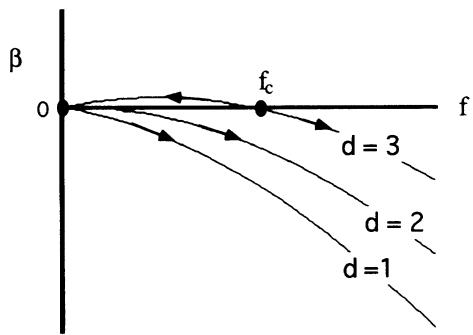
\includegraphics[width=0.55\textwidth]{fig13_1.jpg}
\caption{$\beta$ 函数与 $\Lambda$ 减小时 $f$ 的流动。}
\label{fig:13.1}
\end{figure}

$\bar{\Lambda}$ 向下重整化时，$\beta < 0$ 耦合常数减小，$\beta > 0$ 增大。不动点为

\begin{equation*}
\begin{array}{ll}
d = 1 \; : & f _ {c} = 0 \quad \text{不稳定} \, ,\\
d = 2 \; : & f _ {c} = 0 \quad \text{不稳定} \, ,\\
d = 3 \; : & \left\{ \begin{array}{ll} f _ {c} = 0 & \text{稳定} \\ f _ {c} = \dfrac {2 \pi^ {2}}{n - 2} & \text{不稳定} \end{array} \right. .
\end{array}
\tag{13.46}
\end{equation*}

“稳定”与“不稳定”指 $f \approx f_{c}$ 在重整化下的流动趋向或背离不动点。如图~\ref{fig:13.1} 所示，一维、二维中耦合常数流向强耦合；三维存在弱耦合相与强耦合相。$f < f_{c}$ 时耦合流向弱相互作用不动点——微扰论有效，绕有序基态的低阶自旋波理论成立。如图~\ref{fig:13.1}，$f > f_{c}$ 时体系流向强耦合，即无序。$f_{c}$ 是区分破缺对称相与无序相的临界耦合常数。

深入强耦合相，假设依赖动量的结构因子是光滑的，短程序表现为 $q = 0$ 处的极大：

\begin{equation*}
\frac {1}{\mathcal {N}} \langle \hat {\mathbf {n}} _ {\mathbf {q}} \hat {\mathbf {n}} _ {- \mathbf {q}} \rangle \approx \frac {C}{| \mathbf {q} | ^ {2} + \xi^ {- 2} + \mathcal {O} ( | \mathbf {q} ^ {3} | )} ,
\tag{13.47}
\end{equation*}

$C$ 是有量纲常数。(13.47) 的 Fourier 变换是“Ornstein--Zernicke”关联函数，其在大 $|x|/\xi$ 的渐近形式为\footnote{见 Fisher 的论文，文献注释。}

\begin{equation*}
\langle \hat {\mathbf {n}} ( 0 ) \hat {\mathbf {n}} ( \mathbf {x} ) \rangle \propto | \mathbf {x} | ^ {- ( d - 1 )/2} \exp ( - | \mathbf {x} | / \xi ) \left( 1 + \frac {\xi ( d - 3 )}{| \mathbf {x} |} \right) ,
\tag{13.48}
\end{equation*}

关联长度 $\xi$ 支配关联在远距离的指数衰减，是关联的特征长度尺度。用高截断 $\Lambda$ 与裸耦合 $f(\Lambda)$ 的 NLSM 估算 $\xi$，还是用 $\tilde{\Lambda}$ 与 $f(\tilde{\Lambda})$ 的重整化模型估算，本不应有区别。这一不变性可表述为泛函恒等式：

\begin{equation*}
\xi [ f ( \Lambda ), \Lambda ] = \xi [ f ( \tilde {\Lambda} ), \tilde {\Lambda} ].
\tag{13.49}
\end{equation*}

左端对 $\ln (\tilde{\Lambda})$ 的导数为零，故

\begin{equation*}
\frac {\partial \xi}{\partial \ln ( \tilde {\Lambda} )} + \beta \frac {\partial \xi}{\partial f} = 0.
\tag{13.50}
\end{equation*}

由于 $\xi$ 有距离量纲而 $f$ 无量纲，由量纲分析：

\begin{equation*}
\xi ( \tilde {\Lambda}, f ) = \tilde {\Lambda} ^ {- 1} \phi ( f ) ,
\tag{13.51}
\end{equation*}

$\phi$ 是无量纲函数。于是

\begin{equation*}
\frac {\partial \xi}{\partial \ln ( \tilde {\Lambda} )} = - \xi ,
\tag{13.52}
\end{equation*}

从而 (13.50) 有显式解

\begin{align*}
\int_{\xi_ {0}} ^ {\xi} \frac {d \xi}{\xi} & = \int_{f_ {0}} ^ {f} \frac {d f}{\beta ( f )}\\
\rightarrow \xi & = \xi_ {0} \exp \left( \int_{f_ {0}} ^ {f} \frac {d f}{\beta ( f )} \right) .
\tag{13.53}
\end{align*}

$\xi_{0}$ 与 $f_{0}$ 是积分常数，可由强耦合处的关联长度定出（见稍后讨论）。

三维中 $\beta$ 在 $f_{c}$ 处线性消失，$\xi$ 按幂律发散：

\begin{align*}
\xi^ {d = 3} & \sim \left( \frac {f - f _ {c}}{f _ {0}} \right) ^ {1 / \beta ' ( f _ {c} )} ,\\
\beta ' ( f _ {c} ) & = - 1 + \mathcal {O} ( 1 ) .
\tag{13.54}
\end{align*}

二维中由 (13.44)，$\beta$ 函数在 $f_{c}=0$ 处二次消失。可以从强耦合区（$f_{0} \gg 1$，关联长度 $\xi_{0}=O(a)$）到物理 $f$ 值积分 (13.53) 右端：

\begin{equation*}
\xi^ {d = 2} \sim \xi_ {0} \exp \left( \frac {2 \pi}{( n - 2 ) f} \right).
\tag{13.55}
\end{equation*}

对给定格子模型确定 $\xi_{0}$，可以把 (13.55) 与强耦合（高温）下数值定出的关联长度拟合。$\xi_{0}/a$ 是依赖格子模型短程细节的数值常数\footnote{见 Shenker 与 Tobochnik。}。

一维中 (13.53) 积分给出

\begin{equation*}
\xi^ {d = 1} \sim \frac {\xi_ {0} f _ {0}}{f} ,
\tag{13.56}
\end{equation*}

$\xi_{0}f_{0}$ 是 $\Lambda^{-1}$ 的量级。

\begin{exercises}

\item 对 $O(3)$ 模型，把两个自旋波坐标写成一个复场：

\begin{equation*}
\psi ( \mathbf {x} ) = \phi^ {1} ( \mathbf {x} ) + i \phi^ {2} ( \mathbf {x} ) ,
\tag{13.57}
\end{equation*}

并定义 $U(1)$ 规范场

\begin{equation*}
A _ {\mu} [ \hat {\mathbf {n}} ^ {0} ] = - \frac {i}{2} \tilde {A} ^ {12} [ \hat {\mathbf {n}} ^ {0} ].
\tag{13.58}
\end{equation*}

通过对角化 (13.31) 的 $\mathcal{L}^{(2)}$ 中的二次型，求有限规范势存在时的自旋波本征值 $\epsilon_{n}$：

\begin{equation*}
\int d ^ {d} x \left( \partial_ {\mu} \phi^ {a} + \tilde {A} _ {\mu} ^ {ab} \phi^ {b} \right) ^ {2}.
\tag{13.59}
\end{equation*}

证明 $\epsilon_{n}$ 可由方程

\begin{equation*}
\left( \partial_ {\mu} - i 2 A _ {\mu} \right) ^ {2} \psi_ {n} = \epsilon_ {n} \psi_ {n}.
\tag{13.60}
\end{equation*}

得到。注：(13.60) 描述电磁矢量势 $A_{\mu}$ 存在时电荷为 2 的自由玻色子。

\item 证明对 (13.58) 定义的 $O(3)$ NLSM 规范场 $A(\hat{\mathbf{n}})$：

\begin{equation*}
\left( \partial_ {\mu} A _ {\nu} - \partial_ {\nu} A _ {\mu} \right) = \frac {1}{2} \partial_ {\mu} \hat {\mathbf {n}} \times \partial_ {\nu} \hat {\mathbf {n}} \cdot \hat {\mathbf {n}}
\tag{13.61}
\end{equation*}

\item 对二维体系，假设均匀拓扑密度 $B = \partial_{x} \hat{n} \times \partial_{y} \hat{n} \cdot \hat{n}$（如大 Skyrmion 组态中心附近）。选一方便的规范表达 $A_{x}, A_{y}$，并解 (13.60) 的本征值。提示：用均匀磁场中粒子的 Landau 能级理论\footnote{见 L. D. Landau and E. M. Lifshits, \textit{Quantum Mechanics} (Pergamon Press), p. 457，或见 Auerbach, Larson, and Murthy。}

\end{exercises}

\begin{chapbib}
\item 穷人重整化循 Polyakov 的原始推导：
  A. M. Polyakov, Phys. Lett. B \textbf{59}, 79 (1975)；
  A. M. Polyakov, \textit{Gauge Fields and Strings} (Harwood, 1987), 第二章。
\item 非线性 {$\sigma$} 模型到双圈阶的 $d-2$ 展开计算于
  E. Brézin and J. Zinn-Justin, Phys. Rev. B \textbf{14}, 3110 (1976)。
\item 非线性 {$\sigma$} 模型关联长度的有限格子 Monte Carlo 模拟：
  S. H. Shenker and J. Tobochnik, Phys. Rev. B \textbf{22}, 4462 (1980)。
\item Ornstein--Zernicke 关联函数的 Fourier 变换计算于
  M. E. Fisher, Physica \textbf{28}, 172 (1962)。
\item 二维 NLSM 中的孤子（Skyrmion）由
  T. Skyrme, Proc. R. Soc. London Ser. A \textbf{260}, 127 (1961)；
  A. A. Belavin and A. M. Polyakov, JETP Lett. \textbf{22}, 245 (1975)
  发现。
\item 规范势 $A_{ab}^{\mu}$ 对自旋波谱的影响见
  A. Auerbach, B. Larson, and G. Murthy, Phys. Rev. B \textbf{43}, 11515 (1991)。
\item 二维 $xy$ 模型与涡旋效应：
  J. M. Kosterlitz and D. J. Thouless, J. Phys. C \textbf{6}, 1181 (1973)；
  V. L. Berezinskii, Sov. Phys. JETP \textbf{34}, 610 (1972)。
\end{chapbib}

% 第14章 非线性{$\sigma$}模型：大N
\chapter{非线性 $\sigma$ 模型：大 $N$}

第 13 章在弱耦合 $f \ll 1$ 区域求解了 $d$ 维非线性 {$\sigma$} 模型（NLSM）的关联。弱耦合区域对应 $d$ 维格子上经典 Heisenberg 模型的低温极限。由 Haldane 映射（见第 12 章），它也等价于 $d-1$ 维量子 Heisenberg 反铁磁体的大 $S$ 极限，即半经典极限。本章研究 NLSM 的另一种途径：引入称为 $CP^{N-1}$ 模型的复投影表示，$N$ 为复场数目。物理的 $O(3)$ 模型对应 $N = 2$。大 $N$ 极限基本上由路径积分的鞍点给出，即一个平均场理论。该平均场理论恢复了 13.4 节用穷人标度得到的关联长度 $\xi$。

\section{$CP^1$ 表述}

$O(3)$ NLSM 可以用两个复（旋量）场表示

\begin{equation*}
\mathbf {z} ( \mathbf {x} ) = \left[ z _ {1} ( \mathbf {x} ), z _ {2} ( \mathbf {x} ) \right]
\tag{14.1}
\end{equation*}

使得 $\hat{n}$ 的分量由双线性型给出：

\begin{equation*}
n ^ {\alpha} ( \mathbf {x} ) = \mathbf {z} ^ {\dagger} ( \mathbf {x} ) \sigma^ {\alpha} \mathbf {z} ( \mathbf {x} ) \, , \quad \alpha = x, y, z ,
\tag{14.2}
\end{equation*}

$\sigma^{\alpha}$ 是 $2\times2$ Pauli 矩阵（见 (A.20)）。$\hat{n}$ 的模方条件化为约束

\begin{equation*}
| \hat {\mathbf {n}} | = | \mathbf {z} | ^ {2} = | z _ {1} | ^ {2} + | z _ {2} | ^ {2} = 1.
\tag{14.3}
\end{equation*}

需要一些直截了当的代数来证明：由 (14.2) 与 (14.3) 成立恒等式

\begin{equation*}
\frac {1}{4} \left| \partial_ {\mu} \hat {\mathbf {n}} \right| ^ {2} = \left( \partial_ {\mu} \mathbf {z} ^ {\dagger} \right) \cdot \left( \partial_ {\mu} \mathbf {z} \right) - \left[ \mathcal {A} _ {\mu} ( \mathbf {z} ^ {*}, \mathbf {z} ) \right] ^ {2} ,
\tag{14.4}
\end{equation*}

其中 $\mathcal{A}_{\mu}$ 是双线性型：

\begin{equation*}
\mathcal {A} _ {\mu} \equiv - \frac {i}{2} \left[ \mathbf {z} ^ {\dagger} \partial_ {\mu} \mathbf {z} - \left( \partial_ {\mu} \mathbf {z} ^ {\dagger} \right) \mathbf {z} \right].
\tag{14.5}
\end{equation*}

NLSM 配分函数的测度为

\begin{align*}
\mathcal {D} \hat {\mathbf {n}} & = \prod_{\mathbf {x},\, m = 1,2} \frac {d \operatorname{Re} z _ {m} ( \mathbf {x} ) \, d \operatorname{Im} z _ {m} ( \mathbf {x} )}{\pi} \, \delta \left( | \mathbf {z} | ^ {2} - 1 \right)\\
& \equiv \mathcal {D} ^ {2} \mathbf {z} \, \delta \left( | \mathbf {z} | ^ {2} - 1 \right) .
\tag{14.6}
\end{align*}

于是 $CP^1$ 表示为

\begin{align*}
Z_{\mathrm{NLSM}} & = \int \mathcal {D} ^ {2} \mathbf {z} \, \delta \left( | \mathbf {z} | ^ {2} - 1 \right)\\
& \quad \times \exp \left( - \frac {2 \Lambda^ {d - 2}}{f} \int d ^ {d} x \sum_ {\mu} \left| \left[ \partial_ {\mu} - i \mathcal {A} _ {\mu} ( \mathbf {z} ^ {*}, \mathbf {z} ) \right] \mathbf {z} \right| ^ {2} \right) .
\tag{14.7}
\end{align*}

测度中的约束与作用量中的相互作用是求解 (14.7) 关联时困难的来源。引入实约束场 $\lambda(\mathbf{x})$ 与恒等式

\begin{equation*}
\delta \left( | \mathbf {z} | ^ {2} - 1 \right) = \int \mathcal {D} \lambda \, \exp \left[ i \int d ^ {d} x \, \lambda \left( | \mathbf {z} | ^ {2} - 1 \right) \right]
\tag{14.8}
\end{equation*}

可以替换 $\delta$ 函数约束。再引入辅助规范场 $A_{\mu}$ 并用 Hubbard--Stratonovich 恒等式

\begin{equation*}
\exp \left( c \, \mathcal {A} _ {\mu} ^ {2} \right) = \sqrt {\frac {c}{\pi}} \int_{- \infty} ^ {\infty} d A _ {\mu} \, \exp \left( - c A _ {\mu} ^ {2} - 2 c A _ {\mu} \mathcal {A} _ {\mu} \right)
\tag{14.9}
\end{equation*}

解耦四场相互作用 $\mathcal{A}_{\mu}^{2}$。由 (14.7)、(14.8) 与 (14.9)，配分函数为（相差整体归一化）

\begin{align*}
Z_{CP^{1}} & = \int \mathcal {D} ^ {2} \mathbf {z} \, \mathcal {D} \mathbf {A} \, \mathcal {D} \lambda\\
& \quad \exp \left\{ - \int d ^ {d} x \left[ \frac {2 \Lambda^ {d - 2}}{f} \sum_ {\mu} \left| \left( \partial_ {\mu} - i A _ {\mu} \right) \mathbf {z} \right| ^ {2} - i \lambda \left( | \mathbf {z} | ^ {2} - 1 \right) \right] \right\} .
\tag{14.10}
\end{align*}

\section{大 $N$ 下的 $CP^{N - 1}$ 模型}

先把 $CP^{1}$ 模型推广为 $CP^{N-1}$ 模型：复场数目从 $2$ 扩到 $N$：

\begin{equation*}
\mathbf {z} = \left( z _ {1}, z _ {2}, \dots , z _ {N} \right) \, , \quad N \geq 2.
\tag{14.11}
\end{equation*}

约束 (14.3) 推广为

\begin{equation*}
| \mathbf {z} | ^ {2} = \sum_ {m = 1} ^ {N} | z _ {m} | ^ {2} = \frac {N}{2}.
\tag{14.12}
\end{equation*}

(14.12) 的 $N$ 依赖保证大 $N$ 理论非平凡。于是 (14.10) 推广为

\begin{align*}
Z_{CP^{N - 1}} = \int \mathcal {D} ^ {2} \mathbf {z} \, \mathcal {D} \mathbf {A} \, \mathcal {D} \lambda \, \exp \Big[ - \frac {2 \Lambda^ {d - 2}}{f} \int d ^ {d} x \sum_ {\mu} \left| \left( \partial_ {\mu} - i \mathbf {A} _ {\mu} \right) \mathbf {z} \right| ^ {2}\\
- i \lambda \left( | \mathbf {z} | ^ {2} - \frac {N}{2} \right) \Big] .
\tag{14.13}
\end{align*}

形式上可以积掉 $z$ 场：

\begin{align*}
Z_{CP^{N - 1}} & = \int \mathcal {D} \mathbf {A} \, \mathcal {D} \lambda \, \exp \left( - N \mathcal {S} [ \mathbf {A}, \lambda ] \right) ,\\
\mathcal {S} [ \mathbf {A}, \lambda ] & = \mathrm{Tr} \ln \left[ - \left( \partial_ {\mu} - i A _ {\mu} \right) ^ {2} \right] - \frac {i \Lambda^ {d - 2}}{f} \int d ^ {d} x \, \lambda .
\tag{14.14}
\end{align*}

注意 $N$ 乘的是一个与 $N$ 无关的作用量 $\mathcal{S}$。如附录 E 所释，这使 (14.14) 在大 $N$ 下可以鞍点近似：

\begin{equation*}
Z \approx \exp \left( - N \mathcal {S} [ \mathbf {A} _ {0}, \lambda_ {0} ] \right) Z ' ,
\tag{14.15}
\end{equation*}

鞍点方程为

\begin{equation*}
\left. \frac {\delta \mathcal {S}}{\delta \bar {\mathbf {A}}} \right| _ {\bar {\mathbf {A}} _ {0}, \lambda_ {0}} = \left. \frac {\delta \mathcal {S}}{\delta \lambda} \right| _ {\bar {\mathbf {A}} _ {0}, \lambda_ {0}} = 0.
\tag{14.16}
\end{equation*}

假设鞍点作用量 $S[\bar{\mathbf{A}}_{0}, \lambda_{0}]$ 不破缺规范或平移对称，取

\begin{align*}
\mathbf {A} _ {0} & = 0 ,\\
\lambda_ {0} & = - i \bar {\lambda} .
\tag{14.17}
\end{align*}

鞍点作用量是无相互作用 $z$ 场的自由能：

\begin{equation*}
\mathcal {S} ( 0, \bar {\lambda} ) = \sum_ {\mathbf {k}} \ln \left[ \mathbf {k} ^ {2} + \bar {\lambda} \right] - \frac {\mathcal {N} \Lambda^ {d - 2}}{f} \bar {\lambda}.
\tag{14.18}
\end{equation*}

$\bar{\lambda}$ 的鞍点方程为

\begin{equation*}
\mathcal {N} ^ {- 1} \sum_ {\mathbf {k}} \frac {1}{| \mathbf {k} | ^ {2} + \bar {\lambda}} - \frac {1}{f} = 0 ,
\tag{14.19}
\end{equation*}

给出

\begin{equation*}
\bar {\lambda} = \left\{ \begin{array}{ll} f ^ {2} / 4 & d = 1 \\[2pt] \frac {1}{2} \Lambda^ {2} \exp \left( - \frac {4 \pi}{f} \right) & d = 2 \\[4pt] \frac {1}{2} \Lambda^ {2} \left( \frac {2}{\pi} - \frac {4 \pi}{f} \right) ^ {2} & d = 3 \end{array} \right..
\tag{14.20}
\end{equation*}

定义

\begin{align*}
S ^ {+-} ( \mathbf {x} ) & \equiv \left\langle \left[ \hat {\mathbf {n}} ^ {x} ( 0 ) + i \hat {\mathbf {n}} ^ {y} ( 0 ) \right] \left[ \hat {\mathbf {n}} ^ {x} ( \mathbf {x} ) - i \hat {\mathbf {n}} ^ {y} ( \mathbf {x} ) \right] \right\rangle\\
& \rightarrow \left\langle z _ {m} ^ {*} ( 0 ) z _ {m '} ( 0 ) z _ {m '} ^ {*} ( \mathbf {x} ) z _ {m} ( \mathbf {x} ) \right\rangle\\
& \equiv S ^ {m \neq m '} ( \mathbf {x} ) ,
\tag{14.21}
\end{align*}

把（$N=2$ 的）$O(3)$ 关联函数推广到 $N > 2$。由于各味在鞍点作用量 (14.18) 中解耦：

\begin{align*}
S ^ {m \neq m '} ( \mathbf {x} ) & = \left| G ( \mathbf {x} ) \right| ^ {2} ,\\
G ( \mathbf {x} ) & = Z ^ {- 1} \int \mathcal {D} ^ {2} \mathbf {z} \; \mathbf {z} ^ {\dagger} ( 0 ) \cdot \mathbf {z} ( \mathbf {x} )\\
& \quad \times \exp \left( - \frac {2 \Lambda^ {d - 2}}{f} \sum_ {\mathbf {k}} \left( | \mathbf {k} | ^ {2} + \bar {\lambda} \right) \mathbf {z} _ {\mathbf {k}} ^ {*} \mathbf {z} _ {\mathbf {k}} - \frac {N \mathcal {N} \Lambda^ {d - 2}}{f} \bar {\lambda} \right)\\
& = \mathcal {N} ^ {- 1} \sum_ {\mathbf {k}} \frac {e ^ {- i \mathbf {k} \cdot \mathbf {x}}}{| \mathbf {k} | ^ {2} + \bar {\lambda}} .
\tag{14.22}
\end{align*}

循 (13.48)，Fourier 和在大距离的渐近为

\begin{equation*}
G ( \mathbf {x} ) \sim \text{const} \; | \mathbf {x} | ^ {- ( d - 1 )/2} \exp \left( - | \mathbf {x} | \sqrt {\bar {\lambda}} \right).
\tag{14.23}
\end{equation*}

取 $G(\mathbf{x})$ 的平方，得渐近关联函数

\begin{equation*}
\lim_{| \mathbf {x} | \gg \xi} S ^ {m \neq m '} ( \mathbf {x} ) \sim \text{const} \; | \mathbf {x} | ^ {- ( d - 1 )} \exp ( - | \mathbf {x} | / \xi ) ,
\tag{14.24}
\end{equation*}

其中

\begin{equation*}
\xi = \frac {1}{2 \sqrt {\bar {\lambda}}}.
\tag{14.25}
\end{equation*}

由 (14.20)：

\begin{equation*}
\xi = \left\{ \begin{array}{ll} \dfrac {\Lambda^ {- 1}}{f} & d = 1 \\[6pt] \frac {1}{2} \Lambda^ {- 1} \exp \left( + \frac {2 \pi}{f} \right) & d = 2 \\[6pt] \frac {1}{2} \Lambda^ {- 1} \left( \frac {2}{\pi} - \frac {4 \pi}{f} \right) ^ {- 1} & d = 3 \end{array} \right..
\tag{14.26}
\end{equation*}

这些结果（取 $N = 2$）再现了 $O(3)$ NLSM 由 (13.54) 与 (13.55) 给出的关联长度。也就是说，大 $N$ 近似与弱耦合重整化群结果在单圈阶一致。

显然，$CP^{N-1}$ 的大 $N$ 理论在描述 Heisenberg 模型的主要长波特征上相当不坏。这令人放心，因为凝聚态理论与粒子物理中常把大 $N$ 近似用于物理上有趣的 $N = 2$ 体系\footnote{格子 Heisenberg 模型的大 $N$ 理论见第 16、18 章。}。但必须注意：大 $N$ 近似不能恢复更细致的双圈重整化群结果中 $\xi(f)$ 与 $S^{+-}(\mathbf{x})$ 的前指数依赖。这些差别大概来自 $Z'$——它包含 $1/N$ 展开的更高阶项。

\begin{exercises}

\item 证明对 $CP^1$ 模型

\begin{equation*}
\left( \partial_ {\mu} A _ {\nu} - \partial_ {\nu} A _ {\mu} \right) = \frac {1}{2} \partial_ {\mu} \hat {\mathbf {n}} \times \partial_ {\nu} \hat {\mathbf {n}} \cdot \hat {\mathbf {n}} ,
\tag{14.27}
\end{equation*}

其中 $A(\mathbf{z})$ 是 (14.5) 定义的 $CP^1$ 规范场。

\item 比较 (13.61) 与 (14.27)，证明规范场定义 (13.58) 与 (14.5) 相差一个全导数项。利用这一比较证明：$z$ 旋量的电荷是自旋波模式 $\psi$ 电荷的一半。

\end{exercises}

\begin{chapbib}
\item $CP^{N - 1}$ 模型的 $1/N$ 展开引入于
  A. d'Adda, M. Luscher, and P. di Vecchia, Nucl. Phys. B \textbf{146}, 63 (1978)；\textbf{152}, 125 (1979)。
\item 场论大 $N$ 展开的教学参考书：
  S. Coleman, \textit{Aspects of Symmetry} (Cambridge University Press, 1990), 第八章；
  A. M. Polyakov, \textit{Gauge Fields and Strings} (Harwood, 1987), 第八章。
\end{chapbib}

% 第15章 量子反铁磁体：连续理论结果
\chapter{量子反铁磁体：连续理论结果}

第 12 章我们用 Haldane 映射把 $d$ 维量子 Heisenberg 反铁磁体（QHA）的长波关联与带附加 Berry 相位的 $d+1$ 维非线性 {$\sigma$} 模型（NLSM）的关联联系起来。第 13、14 章用连续近似求出了 $d=1,2,3$ 时 NLSM 的关联长度 $\xi$。

原则上，Haldane 映射在连续近似成立时有效，即

\begin{equation*}
\xi_{\mathrm{NLSM}} \gg \Lambda^ {- 1} \, , \quad \xi_{\mathrm{QHA}} \gg a ,
\tag{15.1}
\end{equation*}

$\Lambda$ 与 $a$ 分别是高动量截断与晶格常量。

在能用第 13、14 章的 NLSM 结果之前，必须理解 Berry 相位项 $e^{i\Upsilon}$ 对 (12.37) 右端的影响。

\section{一维：$\Theta$ 项}

考察一维链的 Berry 相位 $\Upsilon$（(12.28) 定义）。对缓变 $\hat{\mathbf{n}}(x)$，展开该项：

\begin{align*}
\Upsilon^ {d = 1} & = - S \sum_ {i} \left\{ \omega [ \hat {\mathbf {n}} ( x _ {2i} ) ] - \omega [ \hat {\mathbf {n}} ( x _ {2i - 1} ) ] \right\}\\
& = \frac {S}{2} \int \frac {d x}{a} \, \frac {\delta \omega}{\delta \hat {\mathbf {n}}} \cdot \partial_ {x} \hat {\mathbf {n}} \; a\\
& = 2 \pi S \, \Theta [ \hat {\mathbf {n}} ( x, \tau ) ] .
\tag{15.2}
\end{align*}

用 (10.34) 导出 $\Theta$ 的泛函形式：

\begin{equation*}
\Theta = \frac {1}{4 \pi} \int d \tau \int d x \, \left( \hat {\mathbf {n}} \times \partial_ {\tau} \hat {\mathbf {n}} \cdot \partial_ {x} \hat {\mathbf {n}} \right).
\tag{15.3}
\end{equation*}

$\Theta$ 是映射

\begin{equation*}
\hat {\mathbf {n}} : \left\{ \left[ - \frac {L}{2}, \frac {L}{2} \right), [ 0, \beta ) \right\} \rightarrow S ^ {2}
\tag{15.4}
\end{equation*}

的拓扑“绕数”或“Pontryagin 指数”，$S^{2}$ 是单位球面。$\Theta[\hat{n}]$ 是 $\hat{n}$ 值域的面积除以 $4\pi$。若定义域有周期边条件，$\hat{n}$ 必须把球面覆盖整数次，因此 $\Theta$ 必为整数。这个整数是拓扑稳定的：$\hat{n}$ 的任何连续形变都不能改变它。把 $\Theta$ 从 1 变到 0好比把包好的球面展开——除非在包装纸上开洞或撕裂，否则不可能。

$\Theta$ 项也出现在 Green 函数的路径积分表示中（那里 $\tau \to it$，见习题）。作为拓扑不变量，其变分为零，不影响经典运动方程。相位因子 $e^{i2\pi S\Theta}$ 对所有整数自旋为 1，但对半奇整数自旋 $S = \frac{1}{2}, \frac{3}{2}, \ldots$ 可正可负。这在路径积分中引起干涉效应，剧烈地改变基态关联与激发，使之不同于纯 NLSM。

存在交替 Berry 相位时连续理论难以求解。然而由 Lieb--Schultz--Mattis 定理（见 5.2 节）可知，半奇整数自旋链的最低激发能随格点数的倒数消失。由可积 $S = \frac{1}{2}$ 链的 Bethe 解，谱是无能隙的，基态关联的渐近衰减为

\begin{equation*}
\langle \mathbf {S} _ {i} \cdot \mathbf {S} _ {j} \rangle \sim ( - 1 ) ^ {( i - j )} \frac {\left( \ln | i - j | \right) ^ {\frac {1}{2}}}{| i - j |}.
\tag{15.5}
\end{equation*}

于是可以得出结论：$\Theta$ 项摧毁 Haldane 能隙并改变渐近关联\footnote{见 Affleck，及 Shankar 与 Read，文献注释。}。

现在给出拓扑干涉项与基态简并之间关系的一个启发性论证。考虑无自旋粒子在圆环上运动，环被磁通为 $\phi$ 的磁通管穿过，如图~\ref{fig:15.1}。哈密顿量简单地为

\begin{equation*}
\mathcal {H} = \frac {\hbar^ {2}}{2 m} \left( - i \partial_ {x} + \frac {\phi}{L \phi_ {0}} \right) ^ {2} ,
\tag{15.6}
\end{equation*}

$\phi_{0}=hc/me$ 是磁通量子。谱以整数 $n$ 标记（见图~\ref{fig:15.1}）：

\begin{equation*}
E ( n ) = \frac {\hbar^ {2}}{2 m L ^ {2}} \left( n + \frac {\phi}{\phi_ {0}} \right) ^ {2} \, , \quad \pm n = 0, 1, 2 \dots .
\tag{15.7}
\end{equation*}

\begin{figure}[H]
\centering
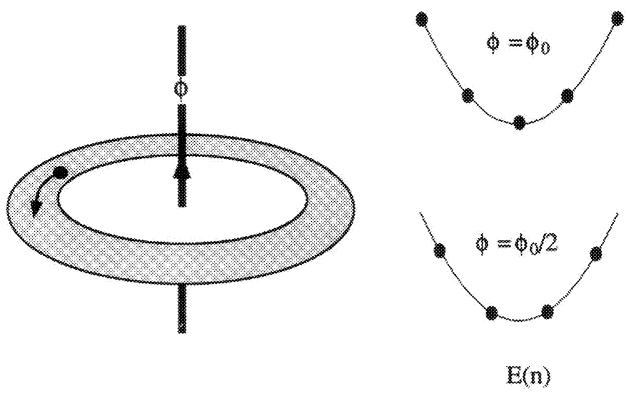
\includegraphics[width=0.5\textwidth]{fig15_1.jpg}
\caption{$\Theta$ 项的类比：环上粒子被磁通管穿过。半奇整数磁通量子导致基态简并。}
\label{fig:15.1}
\end{figure}

对整数 $\phi$，基态

\begin{equation*}
\left| n _ {0} \right\rangle = \left| - \phi / \phi_ {0} \right\rangle
\tag{15.8}
\end{equation*}

非简并。反之，对半奇整数 $\phi/\phi_{0}$，基态是两个简并态

\begin{equation*}
\left| - \phi / \phi_ {0} - \frac {1}{2} \right\rangle \, , \; \left| - \phi / \phi_ {0} + \frac {1}{2} \right\rangle .
\tag{15.9}
\end{equation*}

环上粒子与带 $\Theta$ 项的二维 NLSM 之间的类比，可从 (15.6) 的路径积分表示看出：

\begin{equation*}
Z = \int \mathcal {D} x \, e ^ {i \Upsilon [ x ( \tau ) ]} \exp \left( - \frac {m}{\hbar} \int_ {0} ^ {\beta} d \tau \, \frac {\dot {x} ^ {2}}{2} \right) ,
\tag{15.10}
\end{equation*}

$\Upsilon$ 是粒子与磁通管之间的纯规范耦合（即 Aharonov--Bohm 相位）：

\begin{align*}
\Upsilon & = \frac {2 \pi \phi}{L \phi_ {0}} \int_ {0} ^ {\beta} d \tau \, \dot {x}\\
& = 2 \pi n \frac {\phi}{\phi_ {0}} \, , \quad \pm n = 0, 1, 2 \dots .
\tag{15.11}
\end{align*}

$n$ 是 $x(\tau)$ 的绕数，即粒子绕环的圈数——它是 (15.3) 二维 Pontryagin 指数 $\Theta$ 的一维类比。于是对半奇整数磁通量子 $\phi$ 与半奇整数自旋 $S$，两个体系都在偶、奇拓扑扇区之间发生相消干涉。两个体系中，正是这种干涉造成基态简并。

\section{一维：整数自旋}

由 (15.2)，对整数自旋的一维量子 Heisenberg 反铁磁体可以忽略 Berry 相位因子 $e^{i\Upsilon}$。由 Haldane 映射，QHA 的连续近似是 $d=2$ NLSM，按 13.1 节它是经典 Heisenberg 模型的连续极限。由 Mermin--Wagner 定理 6.2，后者在一切有限温度下无长程序，翻译过来即：QHA 基态对一切 $S < \infty$ 无长程序。

关联长度 $\xi_{\mathrm{NLSM}}(f)$ 已在 (13.55) 求得；大 $N$ 近似 (14.26) 也给出同样结果。于是

\begin{align*}
\xi_{\mathrm{QHA}} ( d = 1, S ) & = \xi_{\mathrm{NLSM}} ( d = 2, f )\\
& \propto a \exp \left( \frac {2 \pi}{f} \right) \, , \quad S = 0, 1, \ldots .
\tag{15.12}
\end{align*}

由表 12.1，近邻模型的耦合常数为

\begin{equation*}
f = 2 / S ,
\tag{15.13}
\end{equation*}

从而

\begin{align*}
\xi_{\mathrm{QHA}} ( S, T = 0 ) & \approx a \exp ( \pi S ) ,\\
\Delta & \approx \frac {c}{a} \exp ( - \pi S )
\tag{15.14}
\end{align*}

$\Delta$ 是 (12.39) 给出的 Haldane 能隙。(15.14) 表明关联长度与 Haldane 能隙对半经典参数是非微扰的——不能按 $1/S$ 幂次从自旋波展开得到。形成对所有激发都有能隙的无序（自旋液体）基态是纯量子现象，没有经典类比；就此而言，它与单个粒子在能量势垒下的隧穿相似\footnote{隧穿率按 $\exp\left[-\frac{1}{\hbar}(\cdot)\right]$ 标度，$\hbar$ 是半经典参数。}。

回顾一维 AKLT Heisenberg 模型（见第 8 章，(8.26)）的基态具有指数衰减的关联 (8.30)；而且在单模近似（见 9.3 节）内我们曾在 (9.21) 估计其能隙。于是，以价键为基态的 $S = 1$ AKLT 模型与其他映射到 NLSM 的整数自旋 Heisenberg 反铁磁体定性相似。由于 AKLT 模型有依赖 $S$ 的相互作用，其在大 $S$ 下的标度行为不同于标准 Heisenberg 模型。

\section{二维}

零温时，正方格子上的 QHA 映射到三维 NLSM。按 (13.46)，后者在

\begin{equation*}
f _ {c} \geq 2 \pi^ {2}
\tag{15.15}
\end{equation*}

处有无序相。对近邻（nn）模型，Neves 与 Perez 证明 $S \geq 1$ 的基态有序。此外，级数展开与数值模拟表明 $S = \frac{1}{2}$ 的基态有序。

遗憾的是，推广 Heisenberg 模型的 $f(S,\Lambda)$ 的精确确定依赖短波正规化方案的细节（即“非普适”）。回忆连续近似本身依赖不等式 (12.10) 与 (15.16)。在临界温度 $T_{c} = f_{c}JS^{2}$ 附近，连近邻关联都大幅退化，在这一区域使用 NLSM 场论是有疑问的。

对连续近似的第一批修正涉及 Néel 场的点奇性。预期这些“刺猬”（hedgehog）在无序相中被热激发。Haldane 证明\footnote{见第 12 章文献注释。}刺猬引入非平凡 Berry 相位 $\Upsilon(2S \bmod 4)$，对 $S=\frac{1}{2},1$ 可能导致基态简并，而对例如 $S=2$ 则否。Read 与 Sachdev 的大 $N$ 途径与 Haldane 的方案一致，并预言由刺猬 Berry 相位引起的自旋 Peierls 有序\footnote{见第 18 章文献注释。}。

由 NLSM 在 $d+1$ 维转动下的对称性，对 $d$ 维动量截断 $\Lambda$，路径积分中最短时间尺度为 $2\pi/(c\Lambda)$。于是在

\begin{equation*}
T \ll c \Lambda
\tag{15.16}
\end{equation*}

区域，可以用宽 $c\beta$ 的有限板上 $d=3$ NLSM 的重整化群方程计算关联长度。Chakravarty、Halperin 与 Nelson（CHN）做到了 $\beta$ 函数的双圈阶。CHN 发现弱耦合区 $f$ 流向 Néel 不动点 $f_{c}=0$，基态有长程序。有限温下他们算得关联长度

\begin{equation*}
\xi_{\mathrm{QHA}} ^ {d = 2} = 0. 9 \, ( c / T ) \exp \left( \frac {2 \pi \rho_ {s}}{T} \right).
\tag{15.17}
\end{equation*}

可以把 $\xi_{\mathrm{QHA}}^{d=2}$ 与 (13.5)、(13.55) 给出的二维 Heisenberg 模型经典结果比较。量子涨落的实质效应是以常数 $Z_{\rho}$ 重整化劲度常数：

\begin{equation*}
\rho_ {s} = Z _ {\rho} \rho_ {s} ^ {cl}.
\tag{15.18}
\end{equation*}

(15.17) 的关联长度称为重整化经典关联。$S = 1/2$ 的 $Z_{\rho}$ 由级数展开算得为 $0.183$\footnote{见 R. R. P. Singh, Phys. Rev. B \textbf{39}, 9760 (1989)。}。

NLSM 对 $S = \frac{1}{2}$ QHA 的许多预言已在准二维 $La_{2}CuO_{4}$ 体系中得到数值与实验的证实。二维中可能的量子无序基态（量子自旋液体）的实验与理论面貌仍未定论。

\begin{chapbib}
\item 带 $\Theta$ 项的 NLSM 对半奇整数 $S$ 无能隙的证明：
  R. Shankar and N. Read, Nucl. Phys. B \textbf{336}, 457 (1990)。
\item 量子自旋链综述：
  I. Affleck, J. Phys. Condensed Matter \textbf{1}, 3047 (1989)。
\item 正方格子上 Heisenberg 反铁磁体 $S \geq 1$ 基态长程序的证明：
  E. J. Neves and J. F. Perez, Phys. Lett. A \textbf{114}, 331 (1986)。
\item 二维有限温关联的重整化群计算：
  S. Chakravarty, B. I. Halperin, and D. Nelson, Phys. Rev. B \textbf{39}, 2344 (1989)。
\item 关于自旋 1/2 二维 Heisenberg 反铁磁体与层状铜氧化物的两篇长篇综述：
  S. Chakravarty, ``High Temperature Superconductivity'', edited by K. S. Bedell, D. Coffey, D. E. Meltzer, D. Pines, and J. R. Schrieffer (Addison-Wesley, 1990)；
  E. Manousakis, Rev. Mod. Phys. \textbf{63}, 1 (1991)。
\end{chapbib}

% 第16章 SU(N) Heisenberg 模型
\chapter{$SU(N)$ Heisenberg 模型}

过去十年间，用大 $N$ 近似处理强相互作用量子体系的工作极为广泛。这一途径起源于基本粒子理论，但在凝聚态物理中找到了众多应用（见文献注释）。最初，大 $N$ 展开是为金属中磁性杂质的 Kondo 与 Anderson 模型发展的；不久之后扩展到稀土化合物中混合价与重费米子现象的 Kondo 与 Anderson 格子模型；也被用于处理高 $T_{c}$ 铜氧化物超导体中的强 Coulomb 相互作用。

在本章及第 17、18 章中，我们将把大 $N$ 途径形式化并应用于量子 Heisenberg 模型。这一方法为量子磁体的静态与动力学关联提供了又一条途径。下面导出的平均场理论既能描述有序相也能描述无序相，零温与有限温皆可，它们与第 11--15 章的半经典途径互为补充。

一般地说，参数 $N$ 标记每个格点上内部 $SU(N)$ 对称的“味”数（即一个 Schwinger 玻色子或受约束费米子可取的味的数目）。多数情况下，大 $N$ 近似被用于处理对称性为 $SU(2)$ 的自旋哈密顿量，因此 $N$ 并不是真正大的参数。尽管如此，$1/N$ 展开提供了得到简单平均场理论的便捷方法。实践发现这些理论或者出奇地成功，或者完全错误，取决于具体体系。例如第 18 章将看到：一维的 Schwinger 玻色子平均场理论对铁磁体和整数自旋反铁磁体行之有效，但对半奇整数自旋反铁磁体则失效。

大 $N$ 途径用约束处理强的局域相互作用。它不是按相互作用大小的微扰展开，而是鞍点展开，通常保持哈密顿量的自旋对称。平均场水平上，约束只在平均意义上被强制；其效应由 $1/N$ 的更高阶修正系统地重新引入。

平均场理论的 $1/N$ 修正可以用 Feynman 图计算，后者描述平均场理论自由准粒子之间的相互作用。17.3 节我们将利用 $1/N$ 展开的独特结构，导出对一切阶成立的某些求和规则。

事实表明，不同的大 $N$ 推广适用于不同的 Heisenberg 模型，取决于耦合符号、自旋大小与格子。“适用”指相应的平均场理论给出基态正确的定性特征。下面引入 Heisenberg 模型的三种大 $N$ 推广，从铁磁体的 Schwinger 玻色子表示开始。

\section{铁磁体：Schwinger 玻色子}

循 7.2 节，每格点引入两个 Schwinger 玻色子 $a_{i}, b_{i}$，并在其 Fock 空间上施加局域约束

\begin{equation*}
a _ {i} ^ {\dagger} a _ {i} + b _ {i} ^ {\dagger} b _ {i} = 2 S.
\tag{16.1}
\end{equation*}

定义键算符

\begin{equation*}
\mathcal {F} _ {ij} \equiv a _ {i} ^ {\dagger} a _ {j} + b _ {i} ^ {\dagger} b _ {j}.
\tag{16.2}
\end{equation*}

自旋 $S$ 的铁磁 Heisenberg 模型写为

\begin{align*}
\mathcal {H} & = - J \sum_{\langle ij \rangle} \mathbf {S} _ {i} \cdot \mathbf {S} _ {j}\\
& = - \frac {J}{2} \sum_{\langle ij \rangle} \left[ \mathcal {F} _ {ij} ^ {\dagger} \mathcal {F} _ {ij} - 2 S ( S + 1 ) \right]\\
& = - \frac {J}{2} \sum_{\langle ij \rangle} \left( : \mathcal {F} _ {ij} ^ {\dagger} \mathcal {F} _ {ij} : - 2 S ^ {2} \right) .
\tag{16.3}
\end{align*}

$\sum_{\langle ij\rangle}$ 对以 $(i,j)$ 为端点的键求和，$: :$ 表示正规排序（见 (C.18)）。把 Schwinger 玻色子的味数从 2 增到 $N$，(16.3) 推广到 $SU(N)$：

\begin{equation*}
\left( a _ {i}, b _ {i} \right) \rightarrow \left( a _ {i 1}, a _ {i 2}, \dots , a _ {iN} \right).
\tag{16.4}
\end{equation*}

键算符推广为

\begin{equation*}
\mathcal {F} _ {ij} \rightarrow \sum_ {m = 1} ^ {N} a _ {im} ^ {\dagger} a _ {jm} ,
\tag{16.5}
\end{equation*}

约束为

\begin{equation*}
\sum_ {m = 1} ^ {N} a _ {im} ^ {\dagger} a _ {im} = NS \, , \quad S = 0, 1, 2, \ldots .
\tag{16.6}
\end{equation*}

$SU(N)$ 铁磁玻色子（FM-B）Heisenberg 模型为

\begin{align*}
\mathcal {H} ^ {\mathrm{FM-B}} ( N ) & = - \frac {J}{N} \sum_{\langle ij \rangle} \left( : \mathcal {F} _ {ij} ^ {\dagger} \mathcal {F} _ {ij} : - NS ^ {2} \right)\\
& = - \frac {J}{N} \sum_ {ij} \left( \sum_ {mm '} S _ {i} ^ {mm '} S _ {j} ^ {m'm} - NS ^ {2} \right) ,
\tag{16.7}
\end{align*}

第二行由重排算符并把 $SU(N)$ 生成元定义为

\begin{equation*}
S ^ {mm '} = a _ {m} ^ {\dagger} a _ {m '}.
\tag{16.8}
\end{equation*}

得到。$S^{mm'}$ 满足 $\mathrm{SU}(N)$ 代数

\begin{equation*}
\left[ S ^ {mm '}, S ^ {\mu \mu '} \right] = \delta_{m' \mu} S^{m \mu '} - \delta_{m \mu '} S^{\mu m'}.
\tag{16.9}
\end{equation*}

特定的“自旋大小” $S$ 由约束 (16.6) 定义。对 $SU(2)$，我们认出通常的自旋算符：$S^{12} = S^{+}$，$S^{21} = S^{-}$，$S^{11} = S^{z} + S$。

可以验证 $H^{\mathrm{FM-B}}$ 在自旋的均匀 $SU(N)$ 变换下不变。我们有意把哈密顿量写成负二次型 $-F_{ij}^{\dagger}F_{ij}$；如将见，这为平均场理论中解耦相互作用提供了自然的出发点。

\section{反铁磁体：Schwinger 玻色子}

考虑子晶格 A、B 的二分格子上近邻反铁磁相互作用 $J > 0$ 的情形。键 $\langle ij\rangle$ 定义为 $i \in A$、$j \in B$。反铁磁键算符定义为

\begin{equation*}
\vec {\mathcal {A}} _ {ij} = a _ {i} b _ {j} - b _ {i} a _ {j}.
\tag{16.10}
\end{equation*}

箭头 $\rightarrow$ 表示对 $i \rightarrow j$ 交换的反对称。在子晶格 B 上定义绕 $y$ 轴转 $\pi$ 的自旋转动：

\begin{equation*}
a _ {j} \rightarrow - b _ {j} \, , \quad b _ {j} \rightarrow a _ {j}.
\tag{16.11}
\end{equation*}

这是保持约束 (16.1) 的正则变换。反铁磁键算符变成对称算符：

\begin{equation*}
\vec {\mathcal {A}} _ {ij} \rightarrow \mathcal {A} _ {ij} = a _ {i} a _ {j} + b _ {i} b _ {j}.
\tag{16.12}
\end{equation*}

$SU(2)$ Heisenberg 模型写为

\begin{align*}
\mathcal {H} & = J \sum_{\langle ij \rangle} \mathbf {S} _ {i} \cdot \mathbf {S} _ {j}\\
& = - \frac {J}{2} \sum_{\langle ij \rangle} \left( \mathcal {A} _ {ij} ^ {\dagger} \mathcal {A} _ {ij} - 2 S ^ {2} \right).
\tag{16.13}
\end{align*}

与铁磁情形一样，可以通过增加 Schwinger 玻色子的味把 $\mathcal{H}$ 推广到 $N > 2$ 模型。约束推广为 (16.6)，键算符推广为

\begin{equation*}
\mathcal {A} _ {ij} \rightarrow \sum_ {m = 1} ^ {N} a _ {im} a _ {jm}.
\tag{16.14}
\end{equation*}

$SU(N)$ 反铁磁玻色子（AFM-B）Heisenberg 模型为

\begin{align*}
\mathcal {H} ^ {\mathrm{AFM-B}} ( N ) & = - \frac {J}{N} \sum_{\langle ij \rangle} \left( \mathcal {A} _ {ij} ^ {\dagger} \mathcal {A} _ {ij} - NS ^ {2} \right)\\
& = - \frac {J}{N} \sum_{\langle ij \rangle} \left( \sum_ {mm '} S _ {i} ^ {mm '} \tilde {S} _ {j} ^ {m'm} - NS ^ {2} \right) ,
\tag{16.15}
\end{align*}

其中

\begin{equation*}
\tilde {S} _ {j} ^ {mm '} = a _ {jm '} ^ {\dagger} a _ {jm}
\tag{16.16}
\end{equation*}

是子晶格 B 上共轭表示的生成元。注意 (16.15) 的 $H^{\mathrm{AFM-B}}$ 在均匀 $SU(N)$ 变换 $U$ 下不变，只在子晶格 A、B 上分别作交错共轭转动 $U$ 与 $U^{\dagger}$ 下不变。

\section{反铁磁体：受约束费米子}

第 2 章我们首次遇到作为电子双线性算符的量子自旋。自旋 1/2 算符可以用每格点两个态 $|i,\uparrow\rangle$、$|i,\downarrow\rangle$ 表示，各被一个费米子占据：

\begin{equation*}
n _ {i \uparrow} + n _ {i \downarrow} = 1 \; ( = 2 S ).
\tag{16.17}
\end{equation*}

由于 Pauli 原理，这一表示限于 $S = \frac{1}{2}$\footnote{$S > \frac{1}{2}$ 的表示可以通过增加轨道与附加约束构造。}。自旋算符为（见 (2.10)）

\begin{align*}
S _ {i} ^ {+} & = c _ {i \uparrow} ^ {\dagger} c _ {i \downarrow} ,\\
S _ {i} ^ {-} & = c _ {i \downarrow} ^ {\dagger} c _ {i \uparrow} ,\\
S _ {i} ^ {z} & = \frac {1}{2} \left( c _ {i \uparrow} ^ {\dagger} c _ {i \uparrow} - c _ {i \downarrow} ^ {\dagger} c _ {i \downarrow} \right) .
\tag{16.18}
\end{align*}

键算符定义为

\begin{equation*}
\mathcal {D} _ {ij} = c _ {i \uparrow} ^ {\dagger} c _ {j \uparrow} + c _ {i \downarrow} ^ {\dagger} c _ {j \downarrow} ,
\tag{16.19}
\end{equation*}

Heisenberg 模型写为

\begin{align*}
\mathcal {H} & = J \sum_{\langle ij \rangle} \mathbf {S} _ {i} \cdot \mathbf {S} _ {j}\\
& = - \frac {J}{2} \sum_{\langle ij \rangle} : \mathcal {D} _ {ij} ^ {\dagger} \mathcal {D} _ {ij} : .
\tag{16.20}
\end{align*}

引入 $N$ 味费米子 $c_{im}$（$m = 1, \ldots, N$），可以把表示 (16.18) 推广到 $\mathrm{SU}(N)$：

\begin{equation*}
S ^ {mm '} = c _ {m} ^ {\dagger} c _ {m '} ,
\tag{16.21}
\end{equation*}

它们满足 $\mathrm{SU}(N)$ 代数 (16.9)。费米子的约束推广为

\begin{equation*}
\sum_ {m = 1} ^ {N} c _ {im} ^ {\dagger} c _ {im} = NS ,
\tag{16.22}
\end{equation*}

$S$ 是广义“自旋大小”。键算符定义为

\begin{equation*}
\mathcal {D} _ {ij} = \sum_ {m} c _ {im} ^ {\dagger} c _ {jm}.
\tag{16.23}
\end{equation*}

$SU(N)$ 反铁磁费米子（AFM-F）Heisenberg 模型由 (16.20) 推广：

\begin{align*}
\mathcal {H} ^ {\mathrm{AFM-F}} ( N ) & = \frac {J}{N} \sum_{\langle ij \rangle} \sum_ {mm '} S _ {i} ^ {mm '} S _ {j} ^ {m'm}\\
& = - \frac {J}{N} \sum_{\langle ij \rangle} : \mathcal {D} _ {ij} ^ {\dagger} \mathcal {D} _ {ij} : .
\tag{16.24}
\end{align*}

\section{生成泛函}

生成哈密顿量定义为

\begin{equation*}
\mathcal {H} [ j ] = \mathcal {H} - \sum_ {imm '} j _ {imm '} ( \tau ) a _ {im} ^ {\dagger} a _ {im '} ,
\tag{16.25}
\end{equation*}

$\tau\in[0,\beta)$ 是虚时间。约束 (16.6) 或 (16.22) 由与 $\mathcal{H}[j]$ 对易的投影算符 $P_{S}$ 强制。虚时生成泛函（见 (D.1)）为

\begin{align*}
Z [ j ] & = \mathrm{Tr} \, P _ {S} T _ {\tau} \left[ \exp \left( - \int_ {0} ^ {\beta} d \tau \, \mathcal {H} [ j ] \right) \right]\\
& = \lim_{\epsilon \to 0} \mathrm{Tr} \, T _ {\tau} \prod_{\tau_ {n} = \epsilon} ^ {\beta} \left[ P _ {S} ( \tau ) \exp \left( - \epsilon \mathcal {H} [ j ( \tau_ {n} ) ] \right) \right] .
\tag{16.26}
\end{align*}

用约束的积分表示

\begin{equation*}
P _ {S} ( \tau ) = \int \mathcal {D} \lambda \, \exp \left[ - i \epsilon \sum_ {im} \lambda_ {i} ( \tau ) \left( a _ {im} ^ {\dagger} a _ {im} - S \right) \right] ,
\tag{16.27}
\end{equation*}

约束场的测度为

\begin{equation*}
\int \mathcal {D} \lambda = \lim_{\epsilon \rightarrow 0} \prod_{i \tau} \epsilon \int_{- \pi / \epsilon} ^ {\pi / \epsilon} d \lambda_{i \tau}.
\tag{16.28}
\end{equation*}

(16.27) 的指数与 $\mathcal{H}[j]$ 可以合并进一个指数，因为它们对易。

循附录 D，为生成泛函构造相干态路径积分，对 Schwinger 玻色子与受约束费米子哈密顿量使用统一记号：

\begin{align*}
Z [ j ] & = \int_{- \infty} ^ {\infty} \mathcal {D} \lambda \int \mathcal {D} ^ {2} \mathbf {z} \; \exp \Bigg\{ - \int_ {0} ^ {\beta} d \tau \Big[ \sum_ {im} z _ {im} ^ {*} \partial_ {\tau} z _ {im} + H [ j ]\\
& \quad + i \sum_ {im} \lambda_ {i} ( \tau ) \left( z _ {im} ^ {*} z _ {im} - S \right) \Big] \Bigg\} ,
\tag{16.29}
\end{align*}

$z$ 对玻色子是复变量，对费米子是 Grassmann 变量。哈密顿量函数为

\begin{equation*}
H [ j ] = - \frac {J}{N} \sum_{\langle ij \rangle} \mathcal {Z} _ {ij} ^ {*} \mathcal {Z} _ {ij} - \sum_ {imm '} j _ {imm '} ( \tau ) z _ {im} ^ {*} z _ {im '} ,
\tag{16.30}
\end{equation*}

其中

\begin{equation*}
\mathcal {Z} = \left\{ \begin{array}{ll} \sum_ {m} z _ {im} ^ {*} z _ {jm} & \mathrm{FM\mbox{-}B} \\ \sum_ {m} z _ {im} z _ {jm} & \mathrm{AFM\mbox{-}B} \\ \sum_ {m} z _ {im} ^ {*} z _ {jm} & \mathrm{AFM\mbox{-}F} \end{array} \right. ,
\tag{16.31}
\end{equation*}

FM-B、AFM-B 与 AFM-F 哈密顿量分别已在 (16.7)、(16.15) 与 (16.24) 定义。

\section{Hubbard--Stratonovich 变换}

Lagrange 量中的双二次（四变量）项无法在路径积分中直接积分。用 Hubbard--Stratonovich 恒等式

\begin{align*}
& \exp \left[ \frac {J}{N} \mathcal {Z} ^ {*} \mathcal {Z} \epsilon \right] = \int_{- \infty} ^ {\infty} d ^ {2} Q\\
& \quad \times \exp \left[ - \left( \mathcal {Z} ^ {*} Q + \mathcal {Z} Q ^ {*} + N \frac {| Q | ^ {2}}{J} \right) \epsilon \right] ,
\tag{16.32}
\end{align*}

其中

\begin{equation*}
d ^ {2} Q \equiv \frac {\epsilon N}{\pi J} \, \mathrm{Re} Q \, d \mathrm{Im} Q .
\tag{16.33}
\end{equation*}

对每个时间步的每条键 $\langle ij\rangle$ 引入复变量 $Q_{ij}(\tau)$，积分测度定义为

\begin{equation*}
\mathcal {D} ^ {2} Q \equiv \prod_{\langle ij \rangle \tau} d ^ {2} Q _ {ij} ( \tau ).
\tag{16.34}
\end{equation*}

用 (16.27)、(16.29) 与 (16.32)：

\begin{align*}
Z [ j ] & = \int \mathcal {D} ^ {2} Q \, \mathcal {D} \lambda \, \mathcal {D} ^ {2} z\\
& \quad \times \exp \left[ - \int_ {0} ^ {\beta} d \tau \left( L [ j ] + N \frac {| Q _ {ij} | ^ {2}}{J} - iNS \sum_ {i} \lambda_ {i} \right) \right] ,
\tag{16.35}
\end{align*}

Lagrange 量对 $z$ 变量是二次的：

\begin{align*}
L [ \mathbf {z} ^ {*}, \mathbf {z}, j ] & = \sum_ {im} z _ {im} ^ {*} \partial_ {\tau} z _ {im} + \sum_{\langle ij \rangle} \left( \mathcal {Z} _ {ij} ^ {\dagger} Q _ {ij} + \mathcal {Z} _ {ij} Q _ {ij} ^ {*} \right)\\
& \quad - \sum_ {imm '} \left( j _ {imm '} + i \lambda_ {i} \delta_{mm '} \right) z _ {im} ^ {*} z _ {im '} .
\tag{16.36}
\end{align*}

对只含 $z^{*}z$ 项的正规 Lagrange 量（如 FM-B 与 AFM-F 情形），Green 函数矩阵 $\hat{G}$ 定义为

\begin{align*}
L & = \mathbf {z} ^ {*} \hat {G} ^ {- 1} [ j ] \mathbf {z} ,\\
\hat {G} ^ {- 1} & = \partial_ {\tau} + \hat {\lambda} + \hat {Q} - \hat {j} ,
\tag{16.37}
\end{align*}

$\partial_{\tau}$ 已在 (D.9) 定义，$\hat{\lambda},\hat{Q},\hat{j}$ 由 (16.36) 读出。

对反常 Lagrange 量（如 AFM-B）：

\begin{align*}
\mathcal {L} & = \left( \mathbf {z} _ {A} ^ {*}, \mathbf {z} _ {B} \right) \hat {G} ^ {- 1} [ j ] \binom{\mathbf {z} _ {A}}{\mathbf {z} _ {B} ^ {*}} ,\\
\hat {G} ^ {- 1} & = \left( \begin{array}{cc} \partial_ {\tau} + \hat {\lambda} - \hat {j} & \hat {Q} \\ \hat {Q} ^ {\dagger} & - \partial_ {\tau} + \hat {\lambda} - \hat {j} \end{array} \right) ,
\tag{16.38}
\end{align*}

$z_{A}, z_{B}$ 分别是子晶格 A、B 的变量。

循 (C.13) 与 (D.11) 积掉 $z$ 变量，得到辅助场的路径积分：

\begin{align*}
Z [ j ] & = \int \mathcal {D} ^ {2} Q \, \mathcal {D} \lambda \, \exp \left[ - N \mathcal {S} [ \lambda, Q, j ] \right]\\
\mathcal {S} & = - \frac {\eta}{N} \mathrm{Tr}_{\tau im} \left( \ln \hat {G} [ j ] \right) + \int_ {0} ^ {\beta} d \tau \left( \sum_{\langle ij \rangle} \frac {| Q _ {ij} | ^ {2}}{J} - iS \sum_ {i} \lambda_ {i} \right) .
\tag{16.39}
\end{align*}

这个表达式是以 $N$ 为大参数的最陡下降展开的出发点。大 $N$ 展开将在第 17、18 章综述。

\section{关联函数}

连通的两自旋关联函数为

\begin{align*}
\tilde {R} ^ {mm '} ( 1, 2 ) & = \left\langle a _ {m, 1} ^ {\dagger} a _ {m ', 1} a _ {m ', 2} ^ {\dagger} a _ {m, 2} \right\rangle\\
& = Z ^ {- 1} \left. \frac {\delta^ {2} \ln Z}{\delta j_{mm', 1} \, \delta j_{m'm, 2}} \right| _ {j = 0}\\
& = Z ^ {- 1} \int \mathcal {D} ^ {2} Q \, \mathcal {D} \lambda \Big[ - N \frac {\delta^ {2} \mathcal {S}}{\delta j_{mm', 1} \, \delta j_{m'm, 2}}\\
& \quad + N ^ {2} \frac {\delta \mathcal {S}}{\delta j_{mm', 1}} \frac {\delta \mathcal {S}}{\delta j_{m'm, 2}} \exp \left( - N \mathcal {S} [ \lambda, Q ] \right) \Big] ,
\tag{16.40}
\end{align*}

1、2 是时空中的点，被积函数中所有泛函都在 $j=0$ 处取值。由 $\mathcal{S}$ 对味指标的对称性，第二项正比于 $\delta_{mm'}$，$\tilde{R}^{m\neq m'}$ 与 $m,m'$ 无关。对 $SU(2)$，FM-B 与 AFM-F 关联与通常自旋关联的关系为

\begin{equation*}
\tilde {R} _ {N = 2} ^ {m \neq m '} ( 1, 2 ) = \left\langle S _ {i _ {1}} ^ {+} ( \tau_ {1} ) S _ {i _ {2}} ^ {-} ( \tau_ {2} ) \right\rangle .
\tag{16.41}
\end{equation*}

AFM-B 情形，子晶格转动 (16.11) 蕴含

\begin{equation*}
\tilde {R} _ {N = 2} ^ {m \neq m '} ( 1, 2 ) = \left\{ \begin{array}{ll} \left\langle S _ {i _ {1}} ^ {+} ( \tau_ {1} ) S _ {i _ {2}} ^ {-} ( \tau_ {2} ) \right\rangle & i _ {1}, i _ {2} \in A \\ - \left\langle S _ {i _ {1}} ^ {+} ( \tau_ {1} ) S _ {i _ {2}} ^ {+} ( \tau_ {2} ) \right\rangle & i _ {1} \in A, i _ {2} \in B \end{array} \right. .
\tag{16.42}
\end{equation*}

\begin{chapbib}
\item 大 $N$ 方法起源于场论，见第 14 章及其文献注释。
\item 相互作用电子的首次大 $N$ 展开应用于 Coqblin--Schrieffer 模型（Kondo 模型的大 $N$ 推广）：
  N. Read and D. Newns, J. Phys. C \textbf{16}, 3273 (1983)。
\item Coleman 把大 $N$ 展开用于 Anderson 模型的从属玻色子表示：
  P. Coleman, Phys. Rev. B \textbf{35}, 5072 (1987)。
\item 用 $1/N$ 展开导出重费米子的 Fermi 液体参数：
  A. Auerbach and K. Levin, Phys. Rev. Lett. \textbf{57}, 877 (1986)；
  A. Millis and P. Lee, Phys. Rev. B \textbf{35}, 3394 (1987)。
\item 大 $N$ 近似在重费米子与铜氧化物超导体中应用的详尽综述：
  A. Hewson, \textit{The Kondo Problem to Heavy Fermions} (Cambridge, 1993)；
  N. E. Bickers, Rev. Mod. Phys. \textbf{59}, 845 (1987)；
  G. Kotliar, \textit{Correlated Electron Systems}, edited by V. J. Emery (World Scientific, 1993)；
  K. Levin, J. H. Kim, J. P. Lu, and Q. Si, Physica C \textbf{175}, 449 (1991)。
\end{chapbib}

% 第17章 大N展开
\chapter{大 $N$ 展开}

第 16 章我们导出了三族 $SU(N)$ Heisenberg 模型的生成泛函与关联函数的泛函积分表示。(16.39) 与 (16.40) 是精确的，但对 $Q$ 与 $\lambda$ 的积分权重 $\exp(-NS)$ 复杂且非 Gauss。路径积分可用附录 E 阐述的最陡下降法展开，$N$ 是大的控制参数。大的 $N$ 压低鞍点附近大涨落的贡献。$N$ 在半经典展开中的角色类似自旋大小 $S$\footnote{见 (10.25)。}。然而与此相反，大 $N$ 平均场理论绝非“经典的”：它包含量子涨落的失序效应。

鞍点组态记作 $\bar{\lambda},\bar{Q}$。固定辅助场后，Gauss 型 Lagrange 量 $L(\bar{\lambda},\bar{Q})$ 描述无相互作用的 $z$ 粒子。$\bar{\lambda},\bar{Q}$ 由鞍点方程\footnote{存在 $Q$ 与 $Q^{*}$ 的鞍点不是复共轭的情形，见 Auerbach 与 Larson。}

\begin{equation*}
\left. \frac {\delta \mathcal {S}}{\delta \lambda_ {i}} \right| _ {\bar {\lambda}, \bar {Q}} = \langle n _ {i} \rangle - S = 0 ,
\tag{17.1}
\end{equation*}

\begin{equation*}
\left. \frac {\delta \mathcal {S}}{\delta Q _ {ij}} \right| _ {\bar {\lambda}, \bar {Q}} = \left. \frac {\delta \mathcal {S}}{\delta Q _ {ij} ^ {*}} \right| _ {\bar {\lambda}, \bar {Q}} = 0
\tag{17.2}
\end{equation*}

确定，通常称为“平均场方程”。$\langle n\rangle$ 表示用鞍点 Lagrange 量 $L(\bar{\lambda},\bar{Q})$ 的平均场期望值。在第 18 章描述的平均场理论中，$\bar{\lambda},\bar{Q}$ 是静态均匀场，即只有两个变分参数，其输入是格子结构、自旋与温度。

粗略地说，平均场理论的物理意义是“最好地”近似 Heisenberg 模型能量与关联的二次 Lagrange 量。但要强调：它不是变分理论。平均场哈密顿量与基态混入了违反局域约束的非物理波函数；平均场激发（“准粒子”）也因含 Schwinger 玻色子或受约束费米子的密度涨落而违反约束。保约束的激发是偶数个准粒子的复合体。局域约束通过场 $\lambda$ 的动力学涨落重新进入理论——这一表述将在 17.3.1 小节精确化。

$Q_{ij}$ 是与准粒子耦合的有效场。其物理解释由平均场方程 (17.2) 给出：

\begin{equation*}
0 = \left. \frac {\delta \mathcal {S}}{\delta Q _ {ij} ^ {*}} \right| _ {\bar {\lambda}, \bar {Q}} \; \Rightarrow \; Q _ {ij} = \left\{ \begin{array}{ll} \frac {J}{N} \langle \mathcal {F} _ {ij} \rangle & \text{FM-B} \\ \frac {J}{N} \langle \mathcal {A} _ {ij} \rangle & \text{AFM-B} \\ \frac {J}{N} \langle \mathcal {D} _ {ij} \rangle & \text{AFM-F} \end{array} \right.
\tag{17.3}
\end{equation*}

于是 $Q_{ij}$ 自洽地依赖键算符的期望值。

\section{涨落与规范场}

本节把讨论限于 Schwinger 玻色子模型 FM-B 与 AFM-B。Hubbard--Stratonovich 场 $Q_{ij}$ 的涨落可用物理自旋关联作半经典诠释。对 $N = 2$，用 7.3 节定义的自旋相干态之间的 $F_{ij}$、$A_{ij}$ 矩阵元即可说明。铁磁键算符给出

\begin{align*}
Q _ {ij} ^ {F} & \Rightarrow \frac {J}{2} \left\langle \hat {\Omega} _ {i} \right|_{S} \left\langle \hat {\Omega} _ {j} \right|_{S - \frac {1}{2}} \mathcal {F} _ {ij} \left| \hat {\Omega} _ {i} \right\rangle_{S - \frac {1}{2}} \left| \hat {\Omega} _ {j} \right\rangle_{S}\\
& = J S \, e ^ {i ( \chi_ {i} - \chi_ {j} )/2} \left( u _ {i} ^ {*} u _ {j} + v _ {i} ^ {*} v _ {j} \right)\\
& = J S \exp \left( - \frac {i}{2} \psi_{ij} ^ {F} \right) \left| ( 1 + \hat {\Omega} _ {i} \cdot \hat {\Omega} _ {j} )/2 \right| ^ {\frac {1}{2}} ,
\tag{17.4}
\end{align*}

$|\hat{\Omega}(\theta,\phi)\rangle_{S}$ 与 $u(\theta,\phi), v(\theta,\phi)$ 分别已在 (7.18) 与 (7.14) 定义，相位 $\psi^{F}$ 由 (7.19) 给出。由 (17.4) 可见，对铁磁关联的自旋 $\hat{\Omega}_{i} \approx \hat{\Omega}_{j}$，$Q$ 取极大。

对缓变组态，$\psi_{ij}^{F}$ 可按自旋偏差展开到线性阶（见 (7.19)）：

\begin{align*}
\psi_{i, i + \delta_ {\mu}} ^ {F} & = - \cos ( \theta_ {i} ) \left( \phi_ {i} - \phi_{i + \delta_ {\mu}} \right) + \chi_ {i} - \chi_{i + \delta_ {\mu}} + \mathcal {O} \left( | \delta_ {\mu} | ^ {2} \right)\\
& \simeq \mathbf {A} ( \hat {\Omega} _ {i} ) \cdot \partial_ {\mu} \hat {\Omega} _ {i} \, | \delta_ {\mu} | .
\tag{17.5}
\end{align*}

$\{\delta_{\mu}\}$ 是格子上的近邻矢量，$\mathbf{A}$ 是 (10.18) 定义的磁单极矢量势，$\chi_{i}$ 是任意规范选择。

连续规范场定义为

\begin{equation*}
A _ {\mu} ( \mathbf {x} _ {i}, \tau ) \equiv \frac {1}{2} \mathbf {A} ( \hat {\Omega} _ {i} ) \cdot \partial_ {\mu} \hat {\Omega} _ {i} \, , \quad \mu = 0, 1, \dots , d ,
\tag{17.6}
\end{equation*}

$\partial_{0} = \partial_{\tau}$。规范不变（“电磁”）场描述手性自旋关联

\begin{equation*}
F _ {\mu \nu} = \partial_ {\mu} A _ {\nu} - \partial_ {\nu} A _ {\mu} = \frac {1}{2} \partial_ {\mu} \hat {\Omega} \times \partial_ {\nu} \hat {\Omega} \cdot \hat {\Omega}.
\tag{17.7}
\end{equation*}

有限值 $F_{\mu\nu} \neq 0$ 蕴含局域自旋关联在 $\mu - \nu$ 平面内的非共面性：$\mu - \nu$ 平面上有限区域内的自旋在单位球上张出有限面积。

反铁磁情形，键算符给出

\begin{align*}
Q _ {ij} ^ {N} & \Rightarrow \frac {J}{2} \left\langle \hat {\Omega} _ {i} \right|_{S - \frac {1}{2}} \left\langle \hat {\Omega} _ {j} \right|_{S - \frac {1}{2}} \mathcal {A} _ {ij} \left| \hat {\Omega} _ {i}, \hat {\Omega} _ {j} \right\rangle_{S} = J S \, e ^ {- i ( \chi_ {j} + \chi_ {i} )/2} \left( u _ {i} v _ {j} - v _ {i} u _ {j} \right)\\
& = J S \exp \left( - \frac {i}{2} \psi_{ij} ^ {N} \right) \left| ( 1 - \hat {\Omega} _ {i} \cdot \hat {\Omega} _ {j} )/2 \right| ^ {\frac {1}{2}} .
\tag{17.8}
\end{align*}

对反铁磁（Néel）关联的自旋 $\hat{\Omega}_{i} \approx -\hat{\Omega}_{j}$，$Q^{N}$ 取极大。Néel 场定义为

\begin{equation*}
\hat {\mathbf {n}} ( \mathbf {x} _ {i} ) \approx \frac {1}{2} \left[ \eta_ {i} \hat {\Omega} _ {i} + ( 2 d ) ^ {- 1} \sum_{\delta_ {\mu}} \eta_{i + \delta_ {\mu}} \hat {\Omega}_{i + \delta_ {\mu}} \right] \, , \quad \eta_ {i} = \left\{ \begin{array}{ll} 1 & i \in A \\ - 1 & i \in B \end{array} \right. .
\tag{17.9}
\end{equation*}

对反铁磁关联的组态，$\hat{n}$ 近似为由 $(\tilde{\theta},\tilde{\phi})$ 参数化的单位矢量场。键相位 $\psi_{ij}^{N}$ 近似为

\begin{align*}
\psi_{i, i + \delta_ {\mu}} ^ {N} & \simeq - \eta_ {i} \cos ( \tilde {\theta} _ {i} ) \left( \tilde {\phi} _ {i} - \tilde {\phi}_{i + \delta_ {\mu}} \right) + \left( \chi_ {i} - \chi_{i + \delta_ {\mu}} \right)\\
& \simeq \eta_ {i} \mathbf {A} ( \hat {\mathbf {n}} ) \cdot \partial_ {\mu} \hat {\mathbf {n}} \, | \delta_ {\mu} | .
\tag{17.10}
\end{align*}

Néel 规范场 $A^{N}$ 按 (17.6) 定义：

\begin{equation*}
A _ {\mu} ^ {N} ( \mathbf {x} _ {i}, \tau ) \equiv \frac {\eta_ {i}}{2} \mathbf {A} ( \hat {\mathbf {n}} ) \cdot \partial_ {\mu} \hat {\mathbf {n}} ,
\tag{17.11}
\end{equation*}

同样 $\partial_{0} = \partial_{\tau}$。Néel“电磁”场描述交错磁化的手性涨落：

\begin{equation*}
F _ {\mu \nu} ^ {N} = \partial_ {\mu} A _ {\nu} ^ {N} - \partial_ {\nu} A _ {\mu} ^ {N} = \frac {1}{2} \partial_ {\mu} \hat {\mathbf {n}} \times \partial_ {\nu} \hat {\mathbf {n}} \cdot \hat {\mathbf {n}}.
\tag{17.12}
\end{equation*}

一维中“电场”$F_{01}^{N}$ 为

\begin{equation*}
F _ {01} ^ {N} = \frac {1}{2} \partial_ {\tau} \hat {\mathbf {n}} \times \partial_ {x} \hat {\mathbf {n}} \cdot \hat {\mathbf {n}} ,
\tag{17.13}
\end{equation*}

右端正比于 $(x,\tau)$ 平面内的“拓扑密度”\footnote{见 15.1 节，及第 13 章习题 2 与 3。}。

$Q_{ij}^{N}$ 的相位与手性 Néel 关联之间的这一联系，有助于理解大 $N$ 途径与半经典连续途径的对应\footnote{见 Read 与 Sachdev，第 18 章文献注释。}。

\section{$1/N$ 展开图}

把绕鞍点的涨落记作

\begin{equation*}
r _ {\alpha} = \left[ i \lambda_ {i} ( \tau ) - \bar {\lambda} \, , \; \operatorname{Re} Q _ {ij} ( \tau ) - \operatorname{Re} \bar {\mathbf {Q}} \, , \; \operatorname{Im} Q _ {ij} ( \tau ) - \operatorname{Im} \bar {Q} \right] ,
\tag{17.14}
\end{equation*}

$\alpha$ 包括场、空间与时间指标。由 (17.1) 与 (17.2)，作用量绕鞍点的 Taylor 展开没有线性项：

\begin{equation*}
\mathcal {S} = \mathcal {S} ^ {(0)} + \frac {1}{2} \mathcal {S}_{\alpha \alpha '} ^ {(2)} r_ {\alpha} r_{\alpha '} + \mathcal {S} ^ {\mathrm{int}} ,
\tag{17.15}
\end{equation*}

重复指标求和。$\mathcal{S}^{\mathrm{int}}$ 含三次及更高阶项：

\begin{equation*}
\mathcal {S} ^ {\mathrm{int}} = \sum_ {n = 3} ^ {\infty} \frac {1}{n !} \mathcal {S}_{\alpha_ {1} \dots \alpha_ {n}} ^ {( n )} r_{\alpha_ {1}} \dots r_{\alpha_ {n}}.
\tag{17.16}
\end{equation*}

$\mathcal{S}^{(n)}$ 确定如下。作用量写为

\begin{align*}
\mathcal {S} & = \mathcal {S} _ {0} + \frac {\eta}{N} \mathrm{Tr} \ln \left( 1 + G _ {0} \sum_ {\alpha} r _ {\alpha} \hat {v} _ {\alpha} \right) ,\\
\mathcal {S} _ {0} & = \frac {\eta}{N} \mathrm{Tr} \ln G _ {0} ^ {- 1} + \int_ {0} ^ {\beta} d \tau \left( \sum_{\langle ij \rangle} \frac {| Q _ {ij} | ^ {2}}{J} - iS \sum_ {i} \lambda_ {i} \right) ,\\
G _ {0} & = \hat {G} ( \bar {Q}, \bar {Q} ^ {*}, \bar {\lambda} ) ,
\tag{17.17}
\end{align*}

$\hat{G}$ 已在 (16.37) 与 (16.38) 定义，$G_{0}$ 是平均场 Green 函数。矩阵 $\hat{v}_{\alpha}$ 是“内顶点”，它保持 $m$ 味指标并把场 $r_{\alpha}$ 连到两个 $G_{0}$。用恒等式

\begin{equation*}
\operatorname{Tr} \ln ( 1 + A ) = - \sum_ {n = 1} ^ {\infty} \frac {( - 1 ) ^ {n}}{n} \operatorname{Tr} ( A ) ^ {n} ,
\tag{17.18}
\end{equation*}

得到显式表达式

\begin{equation*}
\mathcal {S}_{\alpha_ {1} \dots \alpha_ {n}} ^ {( n )} = \frac {( - 1 ) ^ {n + 1}}{n} \, \frac {\eta}{N} \sum_ {P} \eta \, \mathrm{Tr} \left( \hat {v}_{\alpha_ {1}} G _ {0} \dots \hat {v}_{\alpha_ {n}} G _ {0} \right).
\tag{17.19}
\end{equation*}

$\sum_{P}$ 对 $(\alpha_{1},\ldots \alpha_{n})$ 的所有置换求和；迹对空间、时间与 $m$ 味求和。$\mathcal{S}^{(n)}$ 图示为同一 $m$ 指标的平均场 Green 函数构成的、带 $n$ 个内顶点的“回路”，见图~\ref{fig:17.1}。

\begin{figure}[H]
\centering
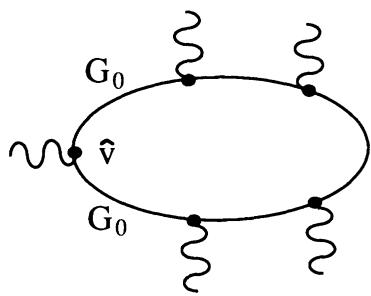
\includegraphics[width=0.45\textwidth]{fig17_1.jpg}
\caption{$\mathcal{S}^{(5)}$——带五个内顶点的回路。}
\label{fig:17.1}
\end{figure}

“RPA 传播子”是二次型的逆：

\begin{equation*}
D _ {\alpha , \alpha '} = \left( \frac {1}{2} \mathcal {S} ^ {(2)} \right)_{\alpha , \alpha '} ^ {- 1} = \left( \Pi_ {0} - \Pi \right)_{\alpha , \alpha '} ^ {- 1} ,
\tag{17.20}
\end{equation*}

其中

\begin{equation*}
\Pi_{\alpha , \alpha '} = \frac {\eta}{N} \operatorname{Tr} \left( \hat {v} _ {\alpha} G _ {0} \hat {v} _ {\alpha '} G _ {0} \right).
\tag{17.21}
\end{equation*}

$\Pi_{0}$ 在动量与 Matsubara 空间是对角的。在辅助场表示（$\mathrm{Re}\, Q, \mathrm{Im}\, Q, \lambda$）中：

\begin{equation*}
\Pi_ {0} = \left( \begin{array}{ccc} \frac {1}{J} & 0 & 0 \\ 0 & \frac {1}{J} & 0 \\ 0 & 0 & 0 \end{array} \right).
\tag{17.22}
\end{equation*}

术语“RPA”（随机相位近似）常用于描述绕平均场理论的 Gauss 涨落。应当始终计算 $\det D$ 以验证

\begin{equation*}
\operatorname{Re} \det D > 0.
\tag{17.23}
\end{equation*}

$\operatorname{Re} \det D$ 的零点与负值是\emph{危险}的：它们使平均场理论不再是一个合法的鞍点。

把 (16.40) 的前置因子与指数按 $r_{\alpha}$ 幂次展开，关联函数由如下求和给出：

\begin{align*}
\tilde {R} ^ {mm '} ( 1, 2 ) & = \tilde {R} ^ {I} ( 1, 2 ) + \delta_{mm '} \tilde {R} ^ {II} ( 1, 2 ) ,\\
\tilde {R} ^ {I} & = Z ^ {- 1} \int \mathcal {D} \mathbf {r} \left( \sum_{n = 0} ^ {\infty} - \frac {1}{n !} \mathcal {S}_{1, 2, \alpha_ {1}, \alpha_ {n}} ^ {( n + 2 )} r_{\alpha_ {1}} \dots r_{\alpha_ {n}} \right)\\
& \quad \times \sum_{L = 0} ^ {\infty} \frac {( - N ) ^ {L}}{L !} \left( \sum_{n = 3} ^ {\infty} \frac {1}{n !} \mathcal {S}_{\alpha_ {1} \ldots \alpha_ {n}} ^ {( n )} r_{\alpha_ {1}} \dots r_{\alpha_ {n}} \right) ^ {L} \exp \left( - \frac {N}{2} \mathcal {S}_{\alpha \beta} ^ {( 2 )} r_{\alpha} r_{\beta} \right) ,
\end{align*}

\begin{figure}[H]
\centering
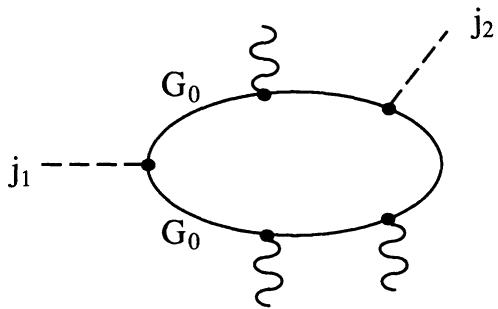
\includegraphics[width=0.45\textwidth]{fig17_2.jpg}
\caption{五个顶点的回路，其中两个是外顶点。}
\label{fig:17.2}
\end{figure}

\begin{align*}
\tilde {R} ^ {II} & = Z ^ {- 1} \int \mathcal {D} \mathbf {r} \left( \sum_{n = 0} ^ {\infty} \frac {1}{n !} \mathcal {S}_{1, \alpha_ {1}, \alpha_ {n}} ^ {( n + 1 )} r_{\alpha_ {1}} \dots r_{\alpha_ {n}} \right) \left( \sum_{n = 0} ^ {\infty} \frac {1}{n !} \mathcal {S}_{2, \alpha_ {1}, \alpha_ {n}} ^ {( n + 1 )} r_{\alpha_ {1}} \dots r_{\alpha_ {n}} \right)\\
& \quad \times \sum_{L = 0} ^ {\infty} \frac {( - N ) ^ {L}}{L !} \left( \sum_{n = 3} ^ {\infty} \frac {1}{n !} \mathcal {S}_{\alpha_ {1} \ldots \alpha_ {n}} ^ {( n )} r_{\alpha_ {1}} \dots r_{\alpha_ {n}} \right) ^ {L} \exp \left( - \frac {N}{2} \mathcal {S}_{\alpha \beta} ^ {( 2 )} r_{\alpha} r_{\beta} \right) ,
\tag{17.24}
\end{align*}

这里略去了作用量中的常数 $-N\mathcal{S}^{(0)}$。定义含一个或两个流顶点的\emph{外回路}（见图~\ref{fig:17.2}）：

\begin{align*}
\frac {\delta}{\delta j _ {m} ( 1 )} \mathcal {S}_{\alpha_ {1}, \alpha_ {n}} ^ {( n )} & = \frac {1}{N} \mathcal {S}_{1, \alpha_ {1}, \alpha_ {n}} ^ {( n + 1 )} ,\\
\frac {\delta^ {2}}{\delta j _ {m} ( 1 ) \delta j _ {m} ( 2 )} \mathcal {S}_{\alpha_ {1}, \alpha_ {n}} ^ {( n )} & = \mathcal {S}_{1, 2, \alpha_ {1}, \alpha_ {n}} ^ {( n + 2 )} .
\tag{17.25}
\end{align*}

(17.24) 中的积分是多维 Gauss 积分之和。Gauss 积分的性质是：偶数个场的积分可写成两两“收缩”之和：

\begin{equation*}
\overbrace {r _ {1} \cdots r _ {2k}} = \sum_{\mathrm{i} _ {1}, \dots \mathrm{i} _ {\mathrm{k}}} \overbrace {r _ {1} r _ {i _ {1}}} \dots \overbrace {r _ {k} r _ {i _ {k}}} ,
\tag{17.26}
\end{equation*}

两个变量的收缩为

\begin{align*}
\widehat {r _ {1} r _ {2}} & \equiv Z ^ {- 1} \int \mathcal {D} \mathbf {r} \; r_{\alpha i \tau} r_{\alpha ' i ' \tau '} \exp \left( - \frac {N}{2} r_{\alpha} D_{\alpha , \beta} ^ {- 1} r_{\beta} \right)\\
& = \frac {1}{N} D_{1, 2}.
\tag{17.27}
\end{align*}

传播子画作连接两个顶点的波浪线，见图~\ref{fig:17.3}。给定回路数目，图按顶点之间以一切可能方式用 $D$ 连接来构造。图的非连通部分包含与外回路 (17.25) 无关的回路；对关联函数只需考虑连通图，因为非连通部分与归一化因子 $Z^{-1}$ 相消——这就是“链簇定理”。于是，计算任何特定图就是：把所有可能的回路与被传播子收缩的顶点相乘，并对内部指标求和。一个重要条件是：内部回路（不含外顶点的）必须至少有三个顶点；外回路可以有任意数目（包括零）的内顶点。任何特定图的 $1/N$ 阶为

\begin{figure}[H]
\centering
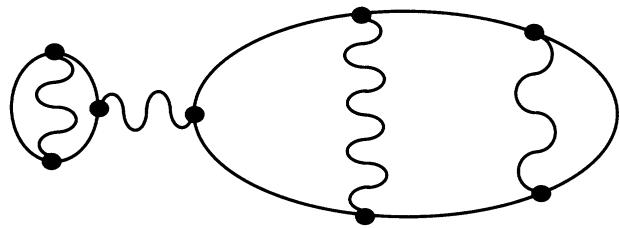
\includegraphics[width=0.5\textwidth]{fig17_3.jpg}
\caption{内场收缩的图。}
\label{fig:17.3}
\end{figure}

\begin{equation*}
\left( \frac {1}{N} \right) ^ {P - L} ,
\tag{17.28}
\end{equation*}

$L$ 是内回路数，$P$ 是传播子数。对 $1/N^{p}$ 阶的所有图求和后得到 $\tilde{R}^{(p)}$——级数的系数：

\begin{equation*}
\tilde {R} ^ {mm '} ( 1, 2 ) \sim \sum_ {p = 0} ^ {\infty} N ^ {- p} \tilde {R} ^ {mm ' (p)} ( 1, 2 ).
\tag{17.29}
\end{equation*}

$\sim$ 表示渐近级数。(17.29) 未必收敛，且可能遗漏 $e^{-N(\cdot)}$ 型的本质奇异项。

\section{求和规则}

$1/N$ 级数的图展开具有特殊结构，使我们能得到在 $1/N$ 级数每一阶都成立的某些恒等式，即求和规则。由 $D$ 的定义本身，无电荷涨落约束逐阶得到强制。下文将分别对 Schwinger 玻色子与受约束费米子展示这一点。此外，我们导出对一切 $N$ 成立的局域 $\mathrm{SU}(N)$ 自旋涨落求和规则。

\subsection{电荷涨落的缺失}

这里证明约束在 $1/N$ 的每一阶都被精确强制。换言之，把给定阶的所有图求和后，密度涨落恒等地消失：

\begin{equation*}
\langle \langle n _ {1} \mathcal {A} \rangle \rangle = NS \, \langle \langle \mathcal {A} \rangle \rangle ,
\tag{17.30}
\end{equation*}

对任意算符 $\mathcal{A}$，$\langle\cdot\rangle$ 是任意温度下的精确期望值。

看看 (17.30) 如何从图展开导出是有启发的。存在相应源流时 Lagrange 量含项

\begin{equation*}
\left( j _ {1} + i \lambda_ {1} \right) \left( \sum_ {m} z _ {1m} ^ {*} z _ {1m} \right) - i \lambda_ {1} NS.
\tag{17.31}
\end{equation*}

对 $j_{1}$ 的外顶点与约束场 $\lambda_{1}$ 的内顶点完全相同。用 (17.25) 对 $\mathcal{S}[j]$ 求两次导：

\begin{equation*}
\mathcal {S}_{1, \alpha} ^ {(2)} = - i \Pi_{\lambda_ {1}, \alpha} ,
\tag{17.32}
\end{equation*}

再由 (17.20) 与 (17.22)：

\begin{equation*}
\sum_ {\alpha} \Pi_{\lambda_ {1}, \alpha} D_{\alpha , \alpha '} = - \left( I _ {\lambda} \right)_{\lambda_ {1}, \alpha '} + \left( \Pi_ {0} D \right)_{\lambda_ {1}, \alpha '} = - \left( I ^ {\lambda} \right)_{\lambda_ {1}, \alpha '} ,
\tag{17.33}
\end{equation*}

$I^{\lambda}$ 投影到 $\lambda$ 场扇区。为了图示地计算 (17.30)，考虑含外回路 $\mathcal{S}^{(n+1)}$（$n \geq 0$）的连通图。先考虑 $n \geq 1$ 的所有图。把一个图的“尾巴”定义为串联附着到回路 $\Pi_{\lambda_{1},r}$（(17.21) 定义）上的一个传播子。所有图可分成两类：有尾巴的与无尾巴的。对每个无尾巴图 $\Gamma(n_{1},\mathcal{A})$，容易通过在 $j_{1}$ 顶点接一个尾巴定义抵消项 $\bar{\Gamma}(n_{1},\mathcal{A})$，如图~\ref{fig:17.4} 所示。由 (17.28)，二者具有相同的 $1/N$ 阶，因为它们的回路数减传播子数相同。用 (17.33) 证明二者精确相消：

\begin{align*}
\bar {\Gamma} ( n _ {1}, \mathcal {A} ) & = N \sum_{\alpha \alpha '} \Pi_{\lambda_ {1} \alpha} D_{\alpha , \alpha '} \Gamma ( n _ {l}, \mathcal {A} )\\
& = \sum_{\alpha '} \left[ - \delta_{\lambda_ {1}, \alpha '} + \sum_{\alpha} \left( \Pi_ {0} \right)_{\lambda_ {1}, \alpha} D_{\alpha , \alpha '} \right] \Gamma ( \alpha ', \mathcal {A} )\\
& = - \Gamma ( n _ {1}, \mathcal {A} ) .
\tag{17.34}
\end{align*}

\begin{figure}[H]
\centering
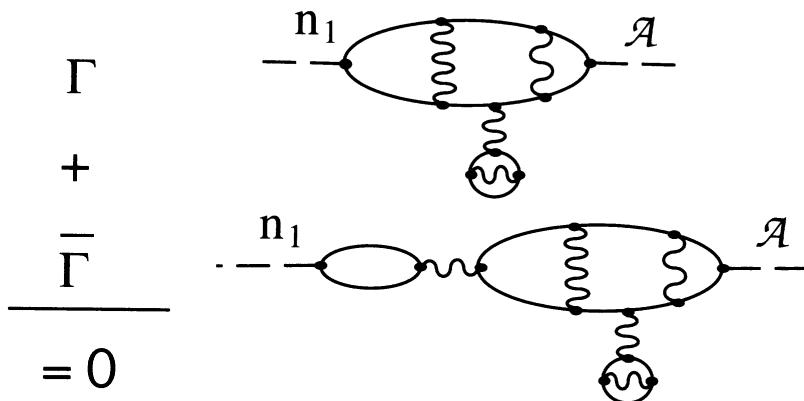
\includegraphics[width=0.45\textwidth]{fig17_4.jpg}
\caption{电荷涨落图及其抵消项。}
\label{fig:17.4}
\end{figure}

于是，在 $1/N$ 的任何阶，抵消项消去电荷涨落图中的连通项。幸存的只有 $n_{1}$ 在回路 $\mathcal{S}^{(1)}$ 上的非连通图。图规则不允许给回路 $N\mathcal{S}^{(1)}$ 加抵消项，因为不可能有只含一两个顶点的内回路。鞍点条件 (17.1) 蕴含

\begin{equation*}
\langle n _ {1} \rangle = NS ,
\tag{17.35}
\end{equation*}

这就完成了 (17.30) 的证明。证毕。

\subsection{在位自旋涨落}

这里计算在位自旋涨落。对 $SU(2)$，我们熟悉“自旋平方”算符 $S^{2}$，投影到 $S$ 扇区后它给出 $S(S+1)$ 倍的单位矩阵。$SU(N)$ 生成元

\begin{equation*}
\hat {S} _ {i} ^ {mm '} = a _ {im} ^ {\dagger} a _ {im '}
\tag{17.36}
\end{equation*}

定义在位涨落

\begin{equation*}
S ^ {mm '} \equiv \langle \langle \hat {S} _ {i} ^ {mm '} \hat {S} _ {i} ^ {m'm} \rangle \rangle ,
\tag{17.37}
\end{equation*}

$\langle\cdot\rangle$ 是任意温度下的精确期望值。利用约束，容易确定“自旋平方”算符的期望值：

\begin{align*}
\sum_ {mm '} S ^ {mm '} & = \left\langle \left\langle \sum_ {mm '} \left[ n_{im '} \left( 1 + \eta n_{im} \right) - \eta \delta_{mm '} n_{im '} \right] \right\rangle \right\rangle\\
& = N ^ {2} S ( 1 + \eta S ) - \eta NS .
\tag{17.38}
\end{align*}

（受约束费米子情形用了恒等式 $n_{im}^2 = n_{im}$。）

\begin{figure}[H]
\centering
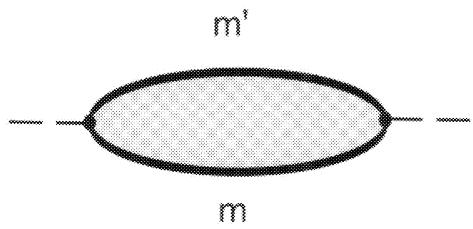
\includegraphics[width=0.45\textwidth]{fig17_5.jpg}
\caption{$S^{m \neq m'}$——所有传播子不可约图之和。}
\label{fig:17.5}
\end{figure}

由于路径积分是 $\mathrm{SU}(N)$ 不变的，可以如下确定单个关联 $S^{mm'}$。先找对角涨落 $S^{mm}$ 与非对角涨落 $S^{m\neq m'}$ 之间的关系。在转动对称的体系中，这些量不能依赖 $m$ 或 $m'$。

由 (17.24)，$S^{m\neq m'}$ 由路径积分 $\tilde{R}^{I}$ 给出。由于内顶点保持 $m$ 指标，$S^{m\neq m'}$ 中的所有图都是连通的，不可能通过剪断任何数目的传播子线分成两部分。把这些图称为传播子不可约（PI）图，见图~\ref{fig:17.5}。构成 $S^{m\neq m'}$ 的所有 PI 图也出现在对角关联 $S_{c}^{mm}$ 的连通部分中：

\begin{equation*}
\text{若} \quad \Gamma^ {PI} \in S ^ {m \neq m '}, \quad \text{则} \quad \Gamma^ {PI} \in S _ {c} ^ {mm}.
\tag{17.39}
\end{equation*}

然而对每个 $\Gamma^{PI}$，$S_{c}^{mm}$ 还含一个带尾巴的抵消项 $\bar{\Gamma}^{PI}$，见图~\ref{fig:17.6}。用 (17.33)，图与抵消项之和为

\begin{align*}
\Gamma^ {PI} ( i, i ) + \bar {\Gamma} ^ {PI} ( i, i ) & = \Gamma^ {PI} ( i, i ) + \sum_{\alpha \alpha '} \bar {\Gamma} _ {\alpha} ^ {PI} ( i, \alpha ) D_{\alpha , \alpha '} \Pi_{\alpha ' \lambda_ {i}}\\
& = \left( 1 - 1/N \right) \Gamma^ {PI} ( i, i ) .
\tag{17.40}
\end{align*}

除 PI 图及其抵消项外，$S_{c}^{mm}$ 还有两个外顶点位于不同回路的贡献——传播子可约（PR）图。但容易证明所有 PR 图与抵消项精确相消（图~\ref{fig:17.7}）：在一个回路上加尾巴，由于变成内回路的那个回路多了一个 $m'$ 求和，抵消项具有相同的 $1/N$ 阶。这就证明了所有不消去的图都是 PI 的。用 (17.38) 得到重要恒等式：

\begin{equation*}
S _ {c} ^ {mm} ( i, i ) = \left( 1 - \frac {1}{N} \right) S ^ {m \neq m '} ( i, i ).
\tag{17.41}
\end{equation*}

\begin{figure}[H]
\centering
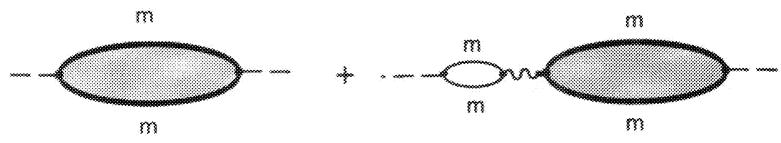
\includegraphics[width=0.45\textwidth]{fig17_6.jpg}
\caption{$S_{\mathrm{c}}^{mm}$——传播子不可约图及其抵消项。}
\label{fig:17.6}
\end{figure}

\begin{figure}[H]
\centering
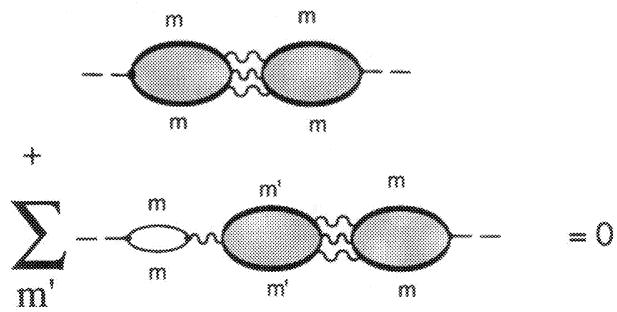
\includegraphics[width=0.45\textwidth]{fig17_7.jpg}
\caption{$S_{\mathrm{c}}^{mm}$——传播子可约图的消去。}
\label{fig:17.7}
\end{figure}

分离 $S^{mm}$ 的连通与非连通部分并用 (17.41)：

\begin{align*}
\sum_ {mm '} S ^ {m, m '} & = \sum_{m \neq m '} S ^ {m \neq m '} ( i, i ) + \sum_{m} \left[ S _ {c} ^ {mm} ( i, i ) + \langle \langle n _ {im} \rangle \rangle ^ {2} \right]\\
& = \left[ N ( N - 1 ) + N \left( 1 - \frac {1}{N} \right) \right] S ^ {m \neq m '} ( i, i ) + NS ^ {2} .
\tag{17.42}
\end{align*}

令 (17.38) 与 (17.42) 相等，得到想要的恒等式

\begin{equation*}
S ^ {m \neq m '} ( 1, 1 ) = \frac {N}{N + \eta} S ( 1 + \eta S ).
\tag{17.43}
\end{equation*}

$N = 2$ 时 (17.43) 化为熟知结果：

\begin{equation*}
\langle S _ {i} ^ {+} S _ {i} ^ {-} \rangle = \left\{ \begin{array}{ll} \frac {2}{3} S ( S + 1 ) & \text{Schwinger 玻色子} \\ \frac {1}{2} & \text{受约束费米子} \end{array} \right.
\tag{17.44}
\end{equation*}

(17.43) 可用于检验 $1/N$ 任意阶的自旋关联图计算。在动量与 Matsubara 频率表示中，$(1/N)^{p}$ 阶的所有图之和必须满足总动量求和规则：

\begin{equation*}
\left( \beta \mathcal {N} \right) ^ {- 1} \sum_{\mathbf {k}, n} S ^ {m \neq m' (p)} ( \mathbf {k}, \omega_ {n} ) = \left( \frac {1}{N} \right) ^ {p} \left( - \eta \right) ^ {p} S ( 1 + \eta S ) \, , \quad p = 0, 1, 2, \dots .
\tag{17.45}
\end{equation*}

\begin{exercises}

\item 计算一维半满 Fermi 气体的自旋关联

\begin{equation*}
\left| \Psi^ {\mathrm{FG}} \right\rangle = \prod_{| k | < \pi / 2} c _ {k \uparrow} ^ {\dagger} c _ {k \downarrow} ^ {\dagger} \left| 0 \right\rangle .
\tag{17.46}
\end{equation*}

提示：证明下列恒等式并计算之：

\begin{equation*}
S ^ {+-} ( q ) = \frac {1}{\mathcal {N}} \sum_ {k} \left\langle c _ {k \uparrow} ^ {\dagger} c_{k + q \downarrow} c_{k + q \downarrow} ^ {\dagger} c _ {k \uparrow} \right\rangle .
\tag{17.47}
\end{equation*}

\item 对 $q$ 求和，计算在位涨落 $\langle S_{i}^{+}S_{i}^{-}\rangle$，与求和规则 (17.44) 比较。解释差异。

\end{exercises}

\begin{chapbib}
\item 大 $N$ 展开中约束的效应，可从 Gutzwiller 投影波函数关联的大 $N$ 展开学习，见第 8 章文献注释。
\item Hubbard--Stratonovich 场 $Q$ 与 $Q^{*}$ 的鞍点不是复共轭的平均场理论讨论于
  A. Auerbach and B. E. Larson, Phys. Rev. B \textbf{43}, 7800 (1991)。
\end{chapbib}

% 第18章 Schwinger 玻色子平均场理论
\chapter{Schwinger 玻色子平均场理论}

本章综述大 $N$ Schwinger 玻色子平均场理论（SBMFT）在 Heisenberg 铁磁体（FM-B）与反铁磁体（AFM-B）于一维及正方格子上的情形。SBMFT（与第 11 章的自旋波理论相反）保持有效哈密顿量显式的 $SU(2)$ 对称\footnote{M. Takahashi 发展了一个类似 SBMFT 但破坏自旋转动对称的修正自旋波理论。}。我们将看到，SBMFT 恢复第 15 章连续途径的主要结果（$\Theta$ 项效应除外）。

下面把 $N$ 保持为独立参数；计算物理 Heisenberg 模型的自旋关联时取 $N \rightarrow 2$。

SBMFT 由把 (16.39) 作用量中的辅助场换成静态均匀鞍点参数给出：

\begin{equation*}
N \mathcal {S} [ Q _ {ij} ( \tau ), \lambda_ {i} ( \tau ) ] \rightarrow N \mathcal {S} _ {0} ( Q, - i \lambda ) = \beta F ^ {\mathrm{MF}} ( Q, \lambda ).
\tag{18.1}
\end{equation*}

$F^{\mathrm{MF}}$ 是平均场自由能，可写为

\begin{equation*}
F ^ {\mathrm{MF}} ( Q, \lambda ) = - \beta^ {- 1} \ln \operatorname{Tr}_{im} \left[ \exp \left( - \beta H ^ {\mathrm{MF}} [ Q, \lambda ] \right) \right] ,
\tag{18.2}
\end{equation*}

$H^{\mathrm{MF}}$ 是 $N$ 味解耦玻色子的平均场哈密顿量。

\section{铁磁体情形}

用 (18.1) 与 (16.36)，无外源流时 FM-B 的平均场哈密顿量为

\begin{align*}
H ^ {\mathrm{MF}} & = \sum_ {im} \lambda \, a _ {im} ^ {\dagger} a _ {im} - Q \sum_{\langle ij \rangle, m} \left( a _ {im} ^ {\dagger} a _ {jm} + a _ {jm} ^ {\dagger} a _ {im} \right)\\
& \quad + N \mathcal {N} \frac {z Q ^ {2}}{2 J} - N \mathcal {N} S \lambda\\
& = \sum_{\mathbf {k}, m} \epsilon_ {\mathbf {k}} \, a _ {\mathbf {k} m} ^ {\dagger} a _ {\mathbf {k} m} + N \mathcal {N} \frac {z Q ^ {2}}{2 J} - N \mathcal {N} S \lambda .
\tag{18.3}
\end{align*}

$\mathcal{N}$ 与 $z$ 分别是格点数与近邻数，$\mathbf{k}$ 是格子动量，而

\begin{align*}
\epsilon_ {\mathbf {k}} & = \lambda - z Q \gamma_ {\mathbf {k}} ,\\
\gamma_ {\mathbf {k}} & = \frac {1}{z} \sum_ {\hat {\eta}} e ^ {i \mathbf {k} \hat {\eta}} .
\tag{18.4}
\end{align*}

$\eta$ 是近邻矢量。

平均场自由能为

\begin{equation*}
F ^ {\mathrm{MF}} = N \sum_ {\mathbf {k}} \ln \left( 1 - e ^ {- \epsilon_{\mathbf {k}} / T} \right) + N \mathcal {N} \frac {z Q ^ {2}}{2 J} - N \mathcal {N} S \lambda .
\tag{18.5}
\end{equation*}

对 $\lambda$ 与 $Q$ 极小化 $F$，得鞍点方程 (17.1) 与 (17.2)：

\begin{equation*}
\frac {1}{\mathcal {N}} \sum_ {\mathbf {k}} n _ {\mathbf {k}} = S ,
\tag{18.6}
\end{equation*}

\begin{equation*}
\frac {1}{\mathcal {N}} \sum_ {\mathbf {k}} n _ {\mathbf {k}} \gamma_ {\mathbf {k}} = Q / J ,
\tag{18.7}
\end{equation*}

其中

\begin{equation*}
n _ {\mathbf {k}} = \frac {1}{e ^ {\epsilon_{\mathbf {k}} / T} - 1}.
\tag{18.8}
\end{equation*}

方程 (18.6) 与 (18.7) 唯一确定平均场参数 $Q(T, S)$ 与 $\lambda(T, S)$。

用平均场变量更具物理意义的参数化是方便的：

\begin{align*}
\epsilon_ {\mathbf {k}} & = z Q \left( 1 - \gamma_ {\mathbf {k}} + \frac {1}{4z} \kappa^ {2} \right) ,\\
\kappa^ {2} & = 4 z \left( \lambda / z Q - 1 \right) .
\tag{18.9}
\end{align*}

$zQ$、$\kappa$ 分别描述带宽与逆关联长度。图~\ref{fig:18.1} 画出一维铁磁体的平均场色散。

从 (18.6) 减去 (18.7)，得 $Q$ 的显式表达式：

\begin{equation*}
Q = J S - \frac {J}{\mathcal {N}} \sum_ {\mathbf {k}} n _ {\mathbf {k}} \left( 1 - \gamma_ {\mathbf {k}} \right).
\tag{18.10}
\end{equation*}

虽然在小宗量处 $n_{\mathbf{k}} \sim (\beta \epsilon_{\mathbf{k}})^{-1}$，右端被积函数在 $k \to 0$ 有界，求和具有 $T$ 的正则幂级数。低温 $T \ll zQ$ 时：

\begin{equation*}
Q = J S + \mathcal {O} ( T / JS ).
\tag{18.11}
\end{equation*}

\begin{figure}[H]
\centering
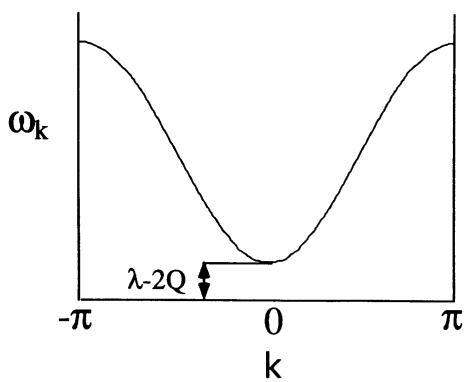
\includegraphics[width=0.55\textwidth]{fig18_1.jpg}
\caption{一维铁磁体的平均场色散。}
\label{fig:18.1}
\end{figure}

有限温时 $\kappa > 0$，$\epsilon_{k}$ 在 $k = 0$ 有大小 $zQ\kappa^{2}/8$ 的能隙。取 $T \to 0$、$\mathcal{N} \to \infty$（热力学极限）时，Bose 函数对所有 $k \neq 0$ 消失。为满足约束方程 (18.6)，$k = 0$ 处必须有宏观占据：

\begin{equation*}
S = \frac {1}{\mathcal {N}} \sum_ {\mathbf {k}} n _ {\mathbf {k}} \sim \frac {1}{\mathcal {N}} n _ {0} = \frac {4 T}{\mathcal {N} J S \kappa^ {2}} + \mathcal {O} ( T ^ {2} ) ,
\tag{18.12}
\end{equation*}

这意味着

\begin{equation*}
\lim_{T \to 0} \kappa = \sqrt {\frac {4 T}{\mathcal {N} J S ^ {2}}}.
\tag{18.13}
\end{equation*}

为研究自旋关联，限于 $N = 2$，并引入 $z$ 方向磁场，它以下列项耦合：

\begin{align*}
H ^ {\mathrm{MF}} & \rightarrow H ^ {\mathrm{MF}} - h \sum_ {i} S _ {i} ^ {z}\\
& = H ^ {\mathrm{MF}} - h \sum_{i, \, s = \pm \frac {1}{2}} s \, a _ {is} ^ {\dagger} a _ {is} .
\tag{18.14}
\end{align*}

场劈裂两个 Schwinger 玻色子色散的简并：

\begin{equation*}
\epsilon_ {\mathbf {k} m} = \epsilon_ {\mathbf {k}} - h s.
\tag{18.15}
\end{equation*}

约束方程给出

\begin{align*}
S & = \frac {1}{2} \lim_{T \to 0} \mathcal {N} ^ {- 1} \sum_ {\mathbf {k}} \left[ n \left( \epsilon_{\mathbf {k}, + \frac {1}{2}} \right) + n \left( \epsilon_{\mathbf {k}, - \frac {1}{2}} \right) \right]\\
& \rightarrow \frac {1}{2} \mathcal {N} ^ {- 1} n \left( \epsilon_{0, + \frac {1}{2}} \right) ,
\tag{18.16}
\end{align*}

磁化为\footnote{见 (6.3)。}

\begin{align*}
m _ {0} & = \frac {1}{2} \mathcal {N} ^ {- 1} \lim_{h \to 0 ^ {+}} \sum_ {\mathbf {k}} \left[ n \left( \epsilon_{\mathbf {k}, + \frac {1}{2}} \right) - n \left( \epsilon_{\mathbf {k}, - \frac {1}{2}} \right) \right]\\
& = \frac {1}{2} \mathcal {N} ^ {- 1} n \left( \epsilon_{0, + \frac {1}{2}} \right) = S.
\tag{18.17}
\end{align*}

于是，在无穷小磁场下，$T=0$ 的 Bose 凝聚发生在 $k=0$、$s=+\frac{1}{2}$。Bose 凝聚是完全的：全部可用的 Schwinger 玻色子密度（每格点 $2S$）都积聚在这一单个模式中。Schwinger 玻色子凝聚体的序参量为

\begin{equation*}
\langle a _ {\mathbf {k} s} \rangle = \langle a _ {\mathbf {k} s} ^ {\dagger} \rangle = \sqrt {2 \mathcal {N} m _ {0}} \; \delta_{s, \frac {1}{2}} \delta_{\mathbf {k}, 0}.
\tag{18.18}
\end{equation*}

这一序参量违反约束（即连接不同自旋的态）。但在平均场理论与 $1/N$ 展开之内它有精确的含义\footnote{见 Hirsch 与 Tang。}。

全部玻色子凝聚到最低态，翻译成自旋态即

\begin{equation*}
\Psi^ {\mathrm{MF}} = \prod_ {i} \left( a _ {i, + \frac {1}{2}} ^ {\dagger} \right) ^ {2S} \left| 0 \right\rangle = \left| S, S, \ldots \right\rangle ,
\tag{18.19}
\end{equation*}

与 Marshall 定理推论 5.6 给出的精确基态一致；见 (5.37)。

注意 SBMFT 色散 $\epsilon_{k}$ 在 $T \rightarrow 0$ 时约化为铁磁自旋波，按（见 (11.49)）

\begin{align*}
\lim_{T \to 0} \epsilon_ {\mathbf {k}} \rightarrow \omega_ {\mathbf {k}} & = z J S \left( 1 - \gamma_ {\mathbf {k}} \right)\\
& \sim J S | \mathbf {k} | ^ {2} + \mathcal {O} \left( | \mathbf {k} | ^ {4} \right)
\tag{18.20}
\end{align*}

消失。$\mathbf{k} = 0$ 处 Schwinger 玻色子能量的消失由 Goldstone 定理预期；见 9.2 节。

磁化率为

\begin{align*}
\chi^ {\mathrm{MF}} & = - \mathcal {N} ^ {- 1} \frac {d ^ {2} F ( h )}{d ^ {2} h} = - \frac {1}{4 \mathcal {N}} \frac {d ^ {2} F ( h )}{d ^ {2} \lambda}\\
& = \frac {1}{4 \mathcal {N} T} \sum_ {\mathbf {k}} n _ {\mathbf {k}} \left( n _ {\mathbf {k}} + 1 \right) .
\tag{18.21}
\end{align*}

平均场自旋关联由自由玻色子表达式给出：

\begin{align*}
\langle S _ {i} ^ {+} S _ {j} ^ {-} \rangle_{\mathrm{MF}} & = \langle a _ {i, + \frac {1}{2}} ^ {\dagger} a_{i, - \frac {1}{2}} a_{j, - \frac {1}{2}} ^ {\dagger} a_{j, + \frac {1}{2}} \rangle\\
& = \left| R _ {ij} \right| ^ {2} + S \delta_{ij} ,\\
R _ {ij} & = \frac {1}{\mathcal {N}} \sum_ {\mathbf {k}} n _ {\mathbf {k}} \, e ^ {i \mathbf {k} \cdot \mathbf {x} _ {ij}} ,
\tag{18.22}
\end{align*}

这里用了恒等式 (18.6)。由 (18.6) 与 (18.22)，局域自旋涨落为

\begin{equation*}
\langle S _ {i} ^ {+} S _ {i} ^ {-} \rangle_{\mathrm{MF}} = \frac {1}{\mathcal {N}} \sum_{\mathbf {k}, \mathbf {k} '} n _ {\mathbf {k}} \left( n _ {\mathbf {k} '} + 1 \right) = S ( S + 1 ).
\tag{18.23}
\end{equation*}

对 $SU(2)$，精确结果当然是 $\frac{2}{3}S(S+1)$。由求和规则 (17.43)，我们验证 (18.23) 恰好给出涨落中正确的 $(1/N)^{0}$ 阶贡献。

\subsection{一维}

一维低温 $T \ll JS$ 时，约束方程 (18.6) 中的求和由小能量、小动量区域主导。小 $k$ 时

\begin{align*}
\epsilon & \approx J S \left( \frac {1}{4} \kappa^ {2} + k ^ {2} + \dots \right) ,\\
n ( \epsilon ) & \approx T / \epsilon .
\tag{18.24}
\end{align*}

低温下把动量上截断换成无穷，得到约束求和的领头阶温度依赖：

\begin{align*}
\mathcal {N} ^ {- 1} \sum_ {\mathbf {k}} n _ {\mathbf {k}} & \sim \frac {T}{J S \pi} \int_ {0} ^ {\infty} d k \, \frac {1}{\frac {1}{4} \kappa^ {2} + k ^ {2}} + \mathcal {O} ( T ^ {2} )\\
& \sim T / ( J S \kappa ) \approx S.
\tag{18.25}
\end{align*}

于是

\begin{equation*}
\kappa \sim T / ( J S ^ {2} ) + \mathcal {O} ( T ^ {2} ).
\tag{18.26}
\end{equation*}

低温磁化率同样由积分的小动量部分主导。把 (18.21) 的项按 $k$ 幂次展开，可算出其领头温度依赖：

\begin{align*}
\chi^ {\mathrm{MF}} & = \frac {1}{2 T} \int_{- \pi} ^ {\pi} \frac {d k}{2 \pi} \, n _ {k} \left( n _ {k} + 1 \right)\\
& \sim \frac {J S ^ {4}}{T ^ {2}}.
\tag{18.27}
\end{align*}

$S = \frac{1}{2}$ Heisenberg 铁磁体的精确磁化率 $\chi$ 已由 Takahashi 用 Bethe 解算出：

\begin{equation*}
\chi^ {S = \frac {1}{2}} \sim \frac {J}{24} T ^ {- 2} \sim \frac {2}{3} \chi^ {\mathrm{MF}}
\tag{18.28}
\end{equation*}

这一 $2/3$ 因子的偏差先前已在局域自旋涨落 (18.23) 中出现。然而在 $\chi$ 这样的长程自旋关联函数中也发现同一因子，令人惊讶。

(18.22) 的 $R_{ij}$ 在大距离下可由被积函数在低动量的行为计算：

\begin{equation*}
R _ {ij} \sim \frac {T}{J S \pi} \int_ {0} ^ {\infty} d k \, \frac {e ^ {i k | i - j |}}{\frac {1}{4} \kappa^ {2} + k ^ {2}} = S \, e ^ {- \frac {1}{2} \kappa | i - j |} ,
\tag{18.29}
\end{equation*}

这里用了 (18.26)。低温大距离下用 (18.6)：

\begin{equation*}
\langle S _ {i} ^ {z} S _ {j} ^ {z} \rangle_{\mathrm{MF}} \sim \frac {1}{2} S ^ {2} e ^ {- | i - j | / \xi} ,
\tag{18.30}
\end{equation*}

确立参数 $\kappa$ 是逆关联长度：

\begin{equation*}
\xi = \kappa^ {- 1} \sim J S ^ {2} / T.
\tag{18.31}
\end{equation*}

这一结果与 M. Fisher 计算的一维经典 Heisenberg 铁磁体精确关联长度一致。

\subsection{二维}

考虑正方格子，$z = 4$。计算动量求和的有用函数是

\begin{equation*}
\rho ( \gamma ) = \mathcal {N} ^ {- 1} \sum_ {\mathbf {k}} \delta \left( \gamma - \gamma_ {\mathbf {k}} \right) = \frac {2}{\pi^ {2}} K \left( 1 - \gamma^ {2} \right) ,
\tag{18.32}
\end{equation*}

它描述正方格子上紧束缚跳跃矩阵的态密度，其中

\begin{equation*}
\gamma_ {\mathbf {k}} = \frac {1}{2} \left( \cos k _ {x} + \cos k _ {y} \right).
\tag{18.33}
\end{equation*}

$K(m)$ 是“第一类完全椭圆积分”\footnote{见 Abramowitz 与 Stegun，p. 590。}：

\begin{align*}
K ( m ) & = \int_ {0} ^ {1} d t \left[ \left( 1 - t ^ {2} \right) \left( 1 - m t ^ {2} \right) \right] ^ {- \frac {1}{2}}\\
& \approx \left\{ \begin{array}{ll} \theta ( m ) \left[ \frac {\pi}{2} + \frac {\pi}{8} m + \mathcal {O} ( m ) ^ {2} \right] & m \ll 1 \\ \frac {1}{2} \ln [ 16 / ( 1 - m ) ] & | 1 - m | \ll 1 \end{array} \right. .
\tag{18.34}
\end{align*}

$\rho(\gamma)$ 的重要特征是 $\gamma = \pm 1$ 处的阶跃不连续与 $\gamma_{k} = 0$ 附近的对数发散。该函数画于图~\ref{fig:18.2}。由于主导的低温关联依赖 $\gamma \approx 1$ 处的 $\rho (\gamma)$，用替换

\begin{figure}[H]
\centering
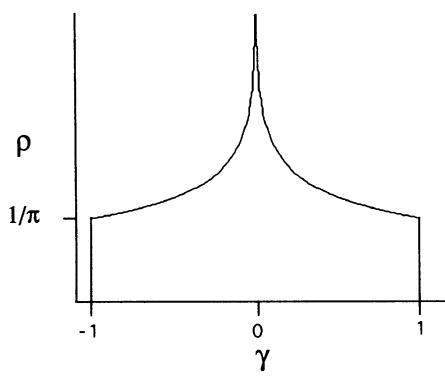
\includegraphics[width=0.55\textwidth]{fig18_2.jpg}
\caption{正方格子上紧束缚色散 $\gamma_{k}$ 的态密度。}
\label{fig:18.2}
\end{figure}

\begin{align*}
\rho ( \gamma ) & \rightarrow \bar {\rho} = \frac {1}{\pi} \, , \quad \gamma \in [ 1 - \pi, 1 ] ,\\
\int_{1 - \pi} ^ {1} d \gamma \, \bar {\rho} ( \gamma ) & = 1 ,
\tag{18.35}
\end{align*}

简化后续计算——延长 $\gamma$ 的定义域以保持单位总密度。用这一相当无害的近似，约束方程容易求解：

\begin{align*}
\mathcal {N} ^ {- 1} \sum_ {\mathbf {k}} n _ {\mathbf {k}} & \approx \frac {T}{4 J S \pi} \int_ {1 - \pi} ^ {1} d \gamma \, \frac {1}{4 ( 1 - \gamma ) + \kappa^ {2} / 4}\\
& = \frac {T}{J S \pi} \ln \left( 16 \pi / \kappa^ {2} \right) + \mathcal {O} ( T ^ {2} ) = S.
\tag{18.36}
\end{align*}

反解此式并用 (18.11)，得领头阶温度解：

\begin{equation*}
\kappa \approx \sqrt {16 \pi} \, \exp \left( \frac {- 2 \pi J S ^ {2}}{T} \right).
\tag{18.37}
\end{equation*}

大距离的自旋关联可用 $R_{ij}$ 的 Ornstein--Zernicke 近似\footnote{见 (13.48)。}计算：

\begin{align*}
R _ {ij} & \approx \frac {T}{J S} \int \frac {d ^ {2} \mathbf {k}}{( 2 \pi ) ^ {2}} \frac {e ^ {i \mathbf {k} \mathbf {x} _ {ij}}}{\frac {1}{4} \kappa^ {2} + k ^ {2}}\\
& \propto \left( | \mathbf {x} _ {ij} | / \xi \right) ^ {- \frac {1}{2}} \exp \left( - | \mathbf {x} _ {ij} | \kappa / 2 \right) \left( 1 + \frac {2}{| \mathbf {x} _ {ij} | \kappa} \dots \right) ,
\tag{18.38}
\end{align*}

$\mathbf{x}_{ij} = \mathbf{x}_i - \mathbf{x}_j$。由 (18.22)：

\begin{equation*}
\langle S _ {i} ^ {z} S _ {j} ^ {z} \rangle_{\mathrm{MF}} \propto \frac {\xi}{| \mathbf {x} _ {ij} |} \, e ^ {- | \mathbf {x} _ {ij} | / \xi} ,
\tag{18.39}
\end{equation*}

其中

\begin{equation*}
\xi = \kappa^ {- 1} \, ,
\tag{18.40}
\end{equation*}

即 $\kappa^{-1}$ 是自旋关联长度。于是我们得出结论：关联长度随温度降低指数增长，且任何有限 $T > 0$ 没有长程序——与 Mermin--Wagner 定理一致。

回忆 13.1 节曾看到，经典 Heisenberg 铁磁体在长距离低温下由耦合常数为

\begin{equation*}
f = \frac {T}{J S ^ {2}}.
\tag{18.41}
\end{equation*}

的非线性 {$\sigma$} 模型描述。(18.37) 恢复了到单圈阶的重整化群结果 (13.55) 与 $CP^{N-1}$ 模型的大 $N$ 近似 (14.26)。

\section{反铁磁体情形}

由 (16.31) 与 (18.2)，AFM-B 表示的平均场哈密顿量为

\begin{align*}
H ^ {\mathrm{MF}} & = \sum_{i, m} \lambda \, a _ {im} ^ {\dagger} a _ {im} + Q \sum_{\langle ij \rangle, m} \left( a _ {im} ^ {\dagger} a _ {jm} ^ {\dagger} + a _ {im} a _ {jm} \right)\\
& \quad + N \mathcal {N} \frac {z Q ^ {2}}{2 J} - N \mathcal {N} S \lambda\\
& = \sum_{\mathbf {k} m} \left[ \lambda \, a _ {\mathbf {k} m} ^ {\dagger} a _ {\mathbf {k} m} + \frac {1}{2} z Q \gamma_ {\mathbf {k}} \left( a _ {\mathbf {k} m} ^ {\dagger} a _ {- \mathbf {k} m} ^ {\dagger} + a _ {\mathbf {k} m} a _ {- \mathbf {k} m} \right) \right]\\
& \quad + N \mathcal {N} \frac {z Q ^ {2}}{2 J} - N \mathcal {N} S \lambda .
\tag{18.42}
\end{align*}

对 $N = 2$，SBMFT 哈密顿量类似于 (11.60) 的 Holstein--Primakoff 自旋波哈密顿量 $H_{1}$，只是这里两个 Schwinger 玻色子味替换了单个 Holstein--Primakoff 玻色子。与自旋波问题极类似，$H^{\mathrm{MF}}$ 可用正则 Bogoliubov 变换对角化：

\begin{equation*}
\alpha_ {\mathbf {k} m} = \cosh \theta_ {\mathbf {k}} \, a _ {\mathbf {k} m} - \sinh \theta_ {\mathbf {k}} \, a _ {- \mathbf {k} m} ^ {\dagger} ,
\tag{18.43}
\end{equation*}

或反解

\begin{equation*}
a _ {\mathbf {k} m} = \cosh \theta_ {\mathbf {k}} \, \alpha_ {\mathbf {k} m} + \sinh \theta_ {\mathbf {k}} \, \alpha_{- \mathbf {k} m} ^ {\dagger}.
\tag{18.44}
\end{equation*}

把 (18.44) 代入 (18.42)，得到 $\alpha$ 玻色子的正规对角哈密顿量：

\begin{align*}
H ^ {\mathrm{MF}} & = \frac {1}{2} \sum_{\mathbf {k} m} \Big[ \left( \lambda \cosh 2 \theta_ {\mathbf {k}} + z Q \gamma_ {\mathbf {k}} \sinh 2 \theta_ {\mathbf {k}} \right) \left( \alpha_{\mathbf {k} m} ^ {\dagger} \alpha_{\mathbf {k} m} + \alpha_{\mathbf {k} m} \alpha_{\mathbf {k} m} ^ {\dagger} \right)\\
& \quad + \left( \lambda \sinh 2 \theta_ {\mathbf {k}} + z Q \gamma_ {\mathbf {k}} \cosh 2 \theta_ {\mathbf {k}} \right) \left( \alpha_{\mathbf {k} m} ^ {\dagger} \alpha_{- \mathbf {k} m} ^ {\dagger} + \alpha_{\mathbf {k} m} \alpha_{- \mathbf {k} m} \right) \Big]\\
& \quad + N \mathcal {N} \frac {z Q ^ {2}}{2 J} - \mathcal {N} N \left( S + \frac {1}{2} \right) \lambda .
\tag{18.45}
\end{align*}

选 $\theta_{\mathbf{k}}$ 使反常项 $\alpha^{\dagger}\alpha^{\dagger}$ 与 $\alpha \alpha$ 消失，即对 $\theta_{\mathbf{k}}$ 的条件：

\begin{equation*}
\tanh 2 \theta_ {\mathbf {k}} = - \frac {z Q \gamma_ {\mathbf {k}}}{\lambda}.
\tag{18.46}
\end{equation*}

解出 $\theta_{k}$ 后，把 (18.45) 中的双曲函数替换为 (18.46) 右端的有理函数，得到正规对角哈密顿量：

\begin{align*}
H ^ {\mathrm{MF}} & = \sum_{\mathbf {k} m} \omega_ {\mathbf {k}} \left( \alpha_{\mathbf {k} m} ^ {\dagger} \alpha_{\mathbf {k} m} + \frac {1}{2} \right) + N \mathcal {N} \frac {z Q ^ {2}}{2 J} - N \mathcal {N} \left( S + \frac {1}{2} \right) \lambda ,\\
\omega_ {\mathbf {k}} & = \sqrt {\lambda^ {2} - \left( z Q \gamma_ {\mathbf {k}} \right) ^ {2}} .
\tag{18.47}
\end{align*}

平均场自由能为

\begin{equation*}
F ^ {\mathrm{MF}} = \beta^ {- 1} \sum_{\mathbf {k} m} \ln \left[ 2 \sinh \left( \frac {\beta \omega_ {\mathbf {k}}}{2} \right) \right] - \mathcal {N} N \left( S + \frac {1}{2} \right) \lambda + N \mathcal {N} \frac {z Q ^ {2}}{2 J}.
\tag{18.48}
\end{equation*}

平均场方程由 (18.48) 对 $\lambda$ 与 $Q$ 求导：

\begin{equation*}
\frac {1}{\mathcal {N}} \sum_ {\mathbf {k}} \frac {\lambda}{\sqrt {\lambda^ {2} - \left( z Q \gamma_ {\mathbf {k}} \right) ^ {2}}} \left( n _ {\mathbf {k}} + \frac {1}{2} \right) = S + \frac {1}{2} ,
\tag{18.49}
\end{equation*}

\begin{equation*}
\frac {1}{\mathcal {N}} \sum_{\mathbf {k}} \frac {z ^ {2} \gamma_{\mathbf {k}} ^ {2} Q}{\sqrt {\lambda^ {2} - \left( z Q \gamma_{\mathbf {k}} \right) ^ {2}}} \left( n _ {\mathbf {k}} + \frac {1}{2} \right) = \frac {z Q}{J}.
\tag{18.50}
\end{equation*}

平均场基态 $\Psi^{\mathrm{MF}}$ 是所有 $\alpha$ 的真空：

\begin{equation*}
\alpha_{\mathbf {k}, m} \Psi_ {0} ^ {\mathrm{MF}} = 0 \, , \quad \forall \mathbf {k}, m.
\tag{18.51}
\end{equation*}

用 (18.43)，可把 $\Psi^{\mathrm{MF}}$ 用原 Schwinger 玻色子显式写出：

\begin{align*}
\Psi^ {\mathrm{MF}} & = C \exp \left[ \frac {1}{2} \sum_ {ij} u _ {ij} \left( \sum_ {m} a _ {im} ^ {\dagger} a _ {jm} ^ {\dagger} \right) \right] \left| 0 \right\rangle ,\\
u _ {ij} & = \frac {1}{\mathcal {N}} \sum_ {\mathbf {k}} e ^ {i \mathbf {k} \mathbf {x} _ {ij}} \tanh \theta_ {\mathbf {k}}.
\tag{18.52}
\end{align*}

$N = 2$ 时，用未转动算符 $a^{\dagger}, b^{\dagger}$，$\Psi^{\mathrm{MF}}$ 就是 Schwinger 玻色子平均场态 (8.5)：

\begin{equation*}
\Psi_{N = 2} ^ {\mathrm{MF}} = \left| \hat {u} \right\rangle = \exp \left[ \sum_{i \in A, \, j \in B} u _ {ij} \left( a _ {i} ^ {\dagger} b _ {j} ^ {\dagger} - b _ {i} ^ {\dagger} a _ {j} ^ {\dagger} \right) \right] \left| 0 \right\rangle .
\tag{18.53}
\end{equation*}

$\Psi^{\mathrm{MF}}$ 含许多占据数不同于 $2S$ 的组态，因此不是纯自旋态。如第 8 章所示，经 Gutzwiller 投影后它化为价键态。由于

\begin{equation*}
\tanh \left( \theta_{\mathbf {k} + \vec {\pi}} \right) = - \tanh \left( \theta_{\mathbf {k}} \right) ,
\tag{18.54}
\end{equation*}

$\vec{\pi} = (\pi, \pi, \ldots)$，键参数 $u_{ij}$ 只连接子晶格 $A$ 与 $B$。而且可以验证，对上述近邻模型 $u_{ij} \geq 0$，故价键态满足 (5.13) 定义的 Marshall 符号。

虽然 $\Psi^{\mathrm{MF}}$ 明显转动不变，却可能有或没有长程反铁磁序——这取决于 $u_{ij}$ 的长距离衰减。我们将看到，近邻模型的 SBMFT 基态在一维无序、二维有长程序。

为进一步计算，引入参数化：

\begin{align*}
\omega_ {\mathbf {k}} & \equiv c \sqrt { ( \kappa / 2 ) ^ {2} + \frac {z}{2} \left( 1 - \gamma_{\mathbf {k}} ^ {2} \right) } ,\\
c & \equiv Q \sqrt {2 z} ,\\
\kappa & \equiv \frac {2}{c} \sqrt {\lambda^ {2} - \left( z Q \right) ^ {2}} ,\\
t & = \frac {T}{z Q}.
\tag{18.55}
\end{align*}

$c$、$\kappa$、$t$ 分别描述自旋波速度、逆关联长度与无量纲温度。图~\ref{fig:18.3} 画出一维反铁磁体的色散。由 (18.48)，在区中心与区角附近，平均场色散是自由有质量相对论性玻色子：

\begin{equation*}
\omega_{\mathbf {k}} ^ {\gamma} \approx c \sqrt { ( \kappa / 2 ) ^ {2} + \left| \mathbf {k} - \mathbf {k} _ {\gamma} \right| ^ {2} } \, , \quad \mathbf {k} _ {\gamma} = 0, \vec {\pi}.
\tag{18.56}
\end{equation*}

当能隙（或“质量” $c\kappa/2$）消失时，$\omega_{k}^{\alpha}$ 是 Goldstone 模，约化为反铁磁自旋波色散 (11.65)。

\begin{figure}[H]
\centering
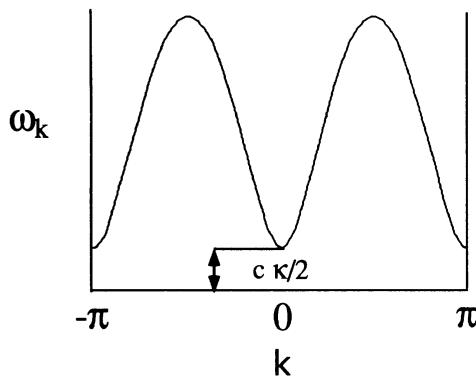
\includegraphics[width=0.55\textwidth]{fig18_3.jpg}
\caption{一维反铁磁体的平均场色散。}
\label{fig:18.3}
\end{figure}

自旋关联函数由在 (16.40) 中用 (18.44) 把 $a$ 算符换成 $\alpha$ 算符得到：

\begin{align*}
S ^ {\mathrm{MF}} ( \mathbf {q} ) & = \frac {1}{\mathcal {N}} \langle S _ {\mathbf {q}} ^ {+} S _ {- \mathbf {q}} ^ {-} \rangle_{\mathrm{MF}}\\
& = \frac {1}{\mathcal {N}} \sum_ {\mathbf {k}} \Bigg\{ \cosh \left[ 2 \left( \theta_{\mathbf {k}} + \theta_{\mathbf {k} + \mathbf {q} + \vec {\pi}} \right) \right]\\
& \quad \times \left( n_{\mathbf {k}} + \frac {1}{2} \right) \left( n_{\mathbf {k} + \mathbf {q} + \vec {\pi}} + \frac {1}{2} \right) - \frac {1}{4} \Bigg\} .
\tag{18.57}
\end{align*}

用 (18.49) 确认求和规则 (17.43) 的大 $N$ 极限：

\begin{equation*}
\frac {1}{\mathcal {N}} \sum_ {\mathbf {q}} S ^ {\mathrm{MF}} ( \mathbf {q} ) = S ( S + 1 ).
\tag{18.58}
\end{equation*}

$N = 2$ 时，平均场求和规则超出精确结果一个熟悉的因子 $\frac{3}{2}$。

自旋关联在 $x_{ij} = x_i - x_j$ 处的空间依赖为

\begin{equation*}
S ^ {\mathrm{MF}} ( \mathbf {x} _ {ij} ) = \left| f ( \mathbf {x} _ {ij} ) \right| ^ {2} - \left| g ( \mathbf {x} _ {ij} ) \right| ^ {2} - \frac {1}{4} \delta_{ij} ,
\tag{18.59}
\end{equation*}

低温长距离下

\begin{align*}
f ( \mathbf {x} _ {ij} ) & = \mathcal {N} ^ {- 1} \sum_ {\mathbf {k}} \frac {\left( n _ {\mathbf {k}} + \frac {1}{2} \right) e ^ {i \mathbf {k} \mathbf {x} _ {ij}}}{\sqrt {1 - \gamma_{\mathbf {k}} ^ {2} \left[ \kappa^ {2} / (2z) + 1 \right] ^ {- 1}}}\\
& \approx 2 z t \left( 1 + e ^ {i \vec {\pi} \mathbf {X} _ {ij}} \right) \int \frac {d ^ {d} \mathbf {k}}{( 2 \pi ) ^ {d}} \frac {e ^ {i \mathbf {k} \mathbf {x} _ {ij}}}{( \kappa / 2 ) ^ {2} + | \mathbf {k} | ^ {2}}\\
& \propto \left( 1 + e ^ {i \vec {\pi} \mathbf {X} _ {ij}} \right) \left( | \mathbf {x} _ {ij} | / \xi \right) ^ {- ( d - 1 )/2} \exp \left( - | \mathbf {x} _ {ij} | \kappa / 2 \right) ,
\tag{18.60}
\end{align*}

小 $\kappa$ 低温下的长距离行为用了 (13.48)。类似地

\begin{align*}
g ( \mathbf {x} _ {ij} ) & = \mathcal {N} ^ {- 1} \sum_ {\mathbf {k}} \gamma_ {\mathbf {k}} \frac {\left( n _ {\mathbf {k}} + \frac {1}{2} \right) e ^ {i \mathbf {k} \mathbf {x} _ {ij}}}{\sqrt {1 - \gamma_{\mathbf {k}} ^ {2} \left[ \kappa^ {2} / (2z) + 1 \right] ^ {- 1}}}\\
& \propto \left( 1 - e ^ {i \vec {\pi} \mathbf {x} _ {ij}} \right) \left( | \mathbf {x} _ {ij} | / \xi \right) ^ {- ( d - 1 )/2} \exp \left( - | \mathbf {x} _ {ij} | \kappa / 2 \right)
\tag{18.61}
\end{align*}

于是对 $\kappa > 0$：

\begin{equation*}
S ^ {\mathrm{MF}} ( \mathbf {x} _ {ij} ) \propto e ^ {i \vec {\pi} \mathbf {x} _ {ij}} \left( \frac {\xi}{| \mathbf {x} _ {ij} |} \right) ^ {d - 1} \exp \left( - | \mathbf {x} _ {ij} | / \xi \right) ,
\tag{18.62}
\end{equation*}

关联长度为 $\xi = \kappa^{-1}$。

均匀磁化率直接由 (18.57) 用恒等式

\begin{equation*}
\chi_ {0} ^ {\mathrm{MF}} = \frac {1}{2 T} S ^ {\mathrm{MF}} ( \mathbf {q} = 0 ) = \frac {1}{T} \sum_ {\mathbf {k}} n _ {\mathbf {k}} \left( n _ {\mathbf {k}} + 1 \right).
\tag{18.63}
\end{equation*}

得到。

\subsection{长程反铁磁序}

没有任何磁场时，基态是单态。在二维及更高维，第 11 章我们看到近邻反铁磁体对所有 $S \geq \frac{1}{2}$ 有长程序。为考察自发破缺对称的可能性，引入耦合到交错磁化的无穷小序场 $h$。限于 $N = 2$：

\begin{align*}
H ^ {\mathrm{MF}} & \rightarrow H ^ {\mathrm{MF}} - h \sum_ {i} S _ {i} ^ {z}\\
& = H ^ {\mathrm{MF}} - h \sum_{i, \, s = - \frac {1}{2}, \frac {1}{2}} s \, a _ {is} ^ {\dagger} a _ {is} ,
\tag{18.64}
\end{align*}

回忆 Schwinger 玻色子在 (16.11) 中是用子晶格转动后的自旋方向定义的。(18.64) 可用依赖自旋的变换角 $\theta_{k,s}$ 对角化。重复导出 (18.47) 的步骤：

\begin{equation*}
\omega_{\mathbf {k}, s} = \sqrt { \left( \lambda - s h \right) ^ {2} - \left( z Q \gamma_{\mathbf {k}} \right) ^ {2} }.
\tag{18.65}
\end{equation*}

自发交错磁化由极限

\begin{align*}
m _ {0} & = \lim_{h \to 0 ^ {+}} m ( h ) \, ,\\
m ( h ) & = \lim_{\mathcal {N} \to \infty} \frac {1}{\mathcal {N}} \sum_{i, s} s \left\langle a _ {is} ^ {\dagger} a _ {is} \right\rangle_{h}\\
& = \lim_{\mathcal {N} \to \infty} \frac {1}{\mathcal {N}} \sum_{\mathbf {k} s} \frac {\lambda - s h}{\sqrt { \left( \lambda - s h \right) ^ {2} - \left( z Q \gamma_{\mathbf {k}} \right) ^ {2} }} \left[ n \left( \omega_{\mathbf {k}, s} \right) + \frac {1}{2} \right]
\tag{18.66}
\end{align*}

给出。约束方程 (18.49) 为

\begin{equation*}
\frac {1}{2 \mathcal {N}} \sum_{\mathbf {k}, s} \frac {\lambda - s h}{\sqrt { \left( \lambda - s h \right) ^ {2} - \left( z Q \gamma_{\mathbf {k}} \right) ^ {2} }} \left[ n \left( \omega_{\mathbf {k}, s} \right) + \frac {1}{2} \right] = S + \frac {1}{2}.
\tag{18.67}
\end{equation*}

再用 $c, \kappa, \tilde{h}$ 参数化色散：

\begin{align*}
\omega_{\mathbf {k}, s} & \equiv c \sqrt { \kappa^ {2} /4 - \left( s - \frac {1}{2} \right) z \tilde {h} + \frac {z}{2} \left( 1 - \gamma_{\mathbf {k}} ^ {2} \right) + \mathcal {O} ( \tilde {h} ^ {2} ) } ,\\
c & = \sqrt {2 z} \, Q ,\\
\kappa & = \frac {2}{c} \sqrt { \left( \lambda - \frac {1}{2} h \right) ^ {2} - \left( z Q \right) ^ {2} } ,\\
\tilde {h} & = h \frac {\lambda}{\left( z Q \right) ^ {2}} .
\tag{18.68}
\end{align*}

若

\begin{equation*}
\lim_{\mathcal {N} \to \infty} \kappa > 0 ,
\tag{18.69}
\end{equation*}

则 (18.66) 中 $s = \pm \frac{1}{2}$ 的两项都在 $h = 0$ 连续，因此

\begin{equation*}
\lim_{h \to 0 ^ {+}} m ( h, \kappa ) = 0 ,
\tag{18.70}
\end{equation*}

即无自发对称破缺。反之，若

\begin{equation*}
\kappa = \mathcal {O} ( \mathcal {N} ) ^ {- 1}
\tag{18.71}
\end{equation*}

则 $k = 0, \vec{\pi}$ 处 $s = +\frac{1}{2}$ 的项贡献 $N$ 阶的量，对交错磁化 (18.66) 给出宏观贡献（即一阶的量）。由于它同时也代表对 Schwinger 玻色子密度 (18.67) 的宏观贡献，可以说 $s = +\frac{1}{2}$ 玻色子在 $k = 0, \vec{\pi}$ 处发生 Bose 凝聚（见 (18.18) 之后的讨论）。凝聚体的序参量于是为

\begin{equation*}
\langle a _ {\mathbf {k} s} \rangle = \langle a _ {\mathbf {k} s} ^ {\dagger} \rangle = \sqrt {\frac {\mathcal {N} m _ {0}}{2}} \; \delta_{s, \frac {1}{2}} \left( \delta_{\mathbf {k}, 0} + \delta_{\mathbf {k}, \vec {\pi}} \right).
\tag{18.72}
\end{equation*}

为计算 $m_0 = \lim_{h\to 0}m(h)$，从 (18.67) 减去 (18.66)，消去发散的 $s = \frac{1}{2}$ 项：

\begin{align*}
m _ {0} & = S + \frac {1}{2}\\
& \quad - \lim_{h \to 0 ^ {+}} \lim_{\mathcal {N} \to \infty} \mathcal {N} ^ {- 1} \sum_ {\mathbf {k}} \frac {2 + 2 \tilde {h} + \kappa^ {2} /4}{\sqrt {2 \tilde {h} + \kappa^ {2} /4 + 2 \left( 1 - \gamma_{\mathbf {k}} ^ {2} \right) }} \left[ n \left( \omega_{\mathbf {k} \frac {1}{2}} \right) + \frac {1}{2} \right].
\tag{18.73}
\end{align*}

保持 $h > 0$ 使谱与被积项分母中有能隙。于是在热力学极限下允许把 (18.73) 换成积分；$T = 0$ 时取 $n(\omega_{\mathbf{k}, + \frac{1}{2}}) = 0$ 与 $\kappa = 0$：

\begin{equation*}
m _ {0} = S + \frac {1}{2} - \frac {1}{2} \int \frac {d ^ {d} \mathbf {k}}{( 2 \pi ) ^ {d}} \frac {1}{\sqrt {1 - \gamma_{\mathbf {k}} ^ {2}}}.
\tag{18.74}
\end{equation*}

对 $d$ 维立方格子，积分给出数值结果

\begin{equation*}
m _ {0} ( d ) = \left\{ \begin{array}{ll} 0 & d = 1 \\ S - 0.19660 & d = 2 \\ S - 0.078 & d = 3 \end{array} \right..
\tag{18.75}
\end{equation*}

注意，与铁磁情形 (18.17) 相反，有序矩总是小于经典值 $S$。这源于量子零点运动——其根源是哈密顿量与交错磁化不可对易。SBMFT 的 $m_{0}$ 结果与 (11.69) 的低阶自旋波理论一致。

\subsection{一维}

零温时取 $n_{\mathbf{k}} = 0$，展开 (18.49)：

\begin{align*}
S + \frac {1}{2} & = \frac {1}{2} \int_{- \pi} ^ {\pi} \frac {d k}{2 \pi} \frac {1}{\sqrt {1 - \frac {1}{1 + \kappa^ {2} /8} \cos^ {2} ( k ) }}\\
& = \frac {1}{\pi} K \left( \frac {1}{1 + \kappa^ {2} /8} \right)\\
& \sim \frac {1}{\pi} \ln \left( \frac {8 \sqrt {2}}{\kappa} \right) + \mathcal {O} ( \kappa ) ,
\tag{18.76}
\end{align*}

得到

\begin{equation*}
\kappa \approx \sqrt {32} \, \exp \left[ - \pi \left( S + \frac {1}{2} \right) \right].
\tag{18.77}
\end{equation*}

(18.75) 中已发现一维反铁磁体的 SBMFT 基态不可能有长程序。由于 $\kappa$ 随 $S$ 指数下降，可以像忽略 $S^{-1}$ 更高阶修正那样忽略 $\kappa$。从 (18.49) 减去 (18.50)：

\begin{align*}
c & = J \left( S + \frac {1}{2} - \frac {1}{2} \int_{- \pi} ^ {\pi} \frac {d k}{2 \pi} \frac {\sin^ {2} k}{\sqrt {\kappa^ {2} /8 + \sin^ {2} k}} \right)\\
& \approx J \left[ S + \frac {1}{2} - \frac {2}{\pi} + \mathcal {O} ( \kappa, S ^ {- 1} ) \right] .
\tag{18.78}
\end{align*}

虽然 $c$ 与其经典值 $c = JS$（见 (11.41)）相去不远，基态关联却按指数衰减。(18.77) 给出的关联长度 $\kappa^{-1}$ 与连续途径 (15.14) 给出的关联长度一致。

平均场激发并非 Heisenberg 模型的物理激发（例如它们包含违反约束的电荷涨落）。但其谱中的能隙 $c\kappa/2$ 与一维整数自旋链 Haldane 能隙的存在一致。物理磁振子谱可从 $\operatorname{Im} S(\mathbf{q},\omega)$ 的峰推得。由于自旋 1 的激发至少涉及两个 Schwinger 玻色子，物理磁振子具有能隙

\begin{equation*}
\Delta = c \kappa .
\tag{18.79}
\end{equation*}

于是，SBMFT 在无 $\Theta$ 项时恢复了 Haldane 的连续理论结果（见第 15 章）。

必须警惕：SBMFT 对半奇整数自旋链失效。摧毁 Haldane 能隙的 $\Theta$ 项 (15.3) 的效应显然在平均场理论中缺席。SBMFT 的非简并基态违反 5.2 节 Lieb--Schultz--Mattis 定理对半奇整数自旋的结论。Read 与 Sachdev 通过在大 $N$ 理论中引入 $\Theta$ 项克服了这一问题；他们为 $Q$、$\lambda$ 涨落发展了一个连续规范理论（见文献注释）。

\subsection{二维}

二维中，由 Mermin--Wagner 定理预期有限温无长程序。的确我们将发现，低温下平均场方程给出有限的逆关联长度 $\kappa(T,S)$。

平均场方程可解出 $\kappa(T, S), c(T, S)$。利用 $\omega_{\mathbf{k}} = \omega(\gamma_{\mathbf{k}})$ 并替换

\begin{equation*}
\frac {1}{\mathcal {N}} \sum_ {\mathbf {k}} F ( \omega_{\mathbf {k}} ) \rightarrow 2 \int_ {0} ^ {1} d \gamma \, \rho ( \gamma ) F [ \omega ( \gamma ) ] ,
\tag{18.80}
\end{equation*}

是方便的，正方格子的 $\rho(\gamma)$ 为

\begin{equation*}
\rho ( \gamma ) = \frac {2}{\pi^ {2}} K \left( 1 - \gamma^ {2} \right).
\tag{18.81}
\end{equation*}

结果表明，温度高于 $T_{max} > 0.91J$ 时，平均场方程无非平凡（$Q \neq 0$）解\footnote{见 Arovas 与 Auerbach。}。这反映了 SBMFT 无法描述高温无序相——那里近邻关联已被摧毁。在关联长度大的温度，即

\begin{equation*}
\kappa \ll t \ll 1 ,
\tag{18.82}
\end{equation*}

约束方程可循 Takahashi 展开：

\begin{align*}
S + \frac {1}{2} & = \frac {1}{2} \int_ {- 1} ^ {1} d \gamma \, \rho ( \gamma ) \left( 1 + \kappa^ {2} /8 - \gamma^ {2} \right) ^ {- \frac {1}{2}} \coth \left[ \left( 1 + \kappa^ {2} /8 - \gamma^ {2} \right) ^ {\frac {1}{2}} / 2t \right]\\
& = \frac {t}{\pi} \left[ \log \left( \frac {32}{\kappa^ {2}} \right) - \log \left( \frac {2}{t} \right) \right]\\
& \quad + \frac {1}{\pi^ {2}} \int_ {- 1} ^ {1} d \gamma \left( 1 - \gamma^ {2} \right) ^ {- \frac {1}{2}} K \left( 1 - \gamma^ {2} \right) + \mathcal {O} ( t, \kappa ) .
\tag{18.83}
\end{align*}

类似地，从 (18.49) 减去 (18.50) 并把积分展开到 $\kappa, t$ 的低阶：

\begin{align*}
& S + \frac {1}{2} - \frac {4 Q}{J}\\
\geq \; & \frac {1}{2} \int_ {- 1} ^ {1} d \gamma \, \rho ( \gamma ) \left( 1 + \kappa^ {2} /8 - \gamma^ {2} \right) ^ {\frac {1}{2}} \coth \left[ \left( 1 + \kappa^ {2} /8 - \gamma^ {2} \right) ^ {\frac {1}{2}} / 2t \right]\\
\approx \; & \frac {1}{\pi^ {2}} \int_ {- 1} ^ {1} d \gamma \left( 1 - \gamma^ {2} \right) ^ {\frac {1}{2}} K \left( 1 - \gamma^ {2} \right) + \mathcal {O} ( t ^ {3}, \kappa ) .
\tag{18.84}
\end{align*}

由 (18.74) 与 (18.75)，有序矩为

\begin{equation*}
m _ {0} = S + \frac {1}{2} - \frac {1}{\pi^ {2}} \int_ {- 1} ^ {1} d \gamma \left( 1 - \gamma^ {2} \right) ^ {- \frac {1}{2}} K \left( 1 - \gamma^ {2} \right) = S - 0.19660.
\tag{18.85}
\end{equation*}

零温自旋波速度为

\begin{equation*}
c = \sqrt {8} \, J S \, Z _ {c} ,
\tag{18.86}
\end{equation*}

自旋波速度重整化因子由 (18.84) 得

\begin{align*}
Z _ {c} & = 1 + S ^ {- 1} \left[ \frac {1}{2} - \frac {1}{\pi^ {2}} \int_ {- 1} ^ {1} d \gamma \left( 1 - \gamma^ {2} \right) ^ {\frac {1}{2}} K \left( 1 - \gamma^ {2} \right) \right]\\
& = 1 + 0.078974 / S .
\tag{18.87}
\end{align*}

渐近自旋关联由 (18.62) 给出，关联长度为 $\xi = \kappa^{-1}$。反解 (18.83) 并用 (18.84)，得到依赖温度的关联长度

\begin{equation*}
\xi = \frac {\sqrt {2} J S Z _ {c}}{T} \exp \left[ - \frac {2 \pi Z _ {c} J S m _ {0}}{T} \right] \left[ 1 + \mathcal {O} ( t ^ {2} ) \right].
\tag{18.88}
\end{equation*}

把 (18.88) 与连续近似值\footnote{见 Chakravarty、Halperin 与 Nelson，第 15 章文献注释。}(15.17) 比较，可以如下确定正方格子模型的重整化劲度常数 $\rho_{s}(S)$：

\begin{equation*}
\rho_ {s} = \lim_{T \to 0} \frac {T}{2 \pi} \log ( \xi ) = J S m _ {0} Z _ {c} ,
\tag{18.89}
\end{equation*}

$m_{0}$ 与 $Z_{c}$ 分别由 (18.85) 与 (18.87) 给出。大 $S$ 极限下它正确恢复经典值 $\rho_{s} \rightarrow JS^{2}$。

\begin{exercises}

\item 用零温下 $Q$ 与 $\lambda$ 的显式解，证明 FM-B 与 AFM-B 平均场理论的基态能量为

\begin{equation*}
E ^ {\mathrm{MF}} = \lim_{T \to 0} F ^ {\mathrm{MF}} = - N \mathcal {N} \frac {z Q ^ {2}}{2 J}.
\tag{18.90}
\end{equation*}

加上从哈密顿量中丢掉的常数 $zNJS^{2}/2$（见 (16.7)），证明 $N = 2$ 时恢复正确的铁磁基态能量。

\item 证明反铁磁 SBMFT 的交错磁场项 (18.64) 导致 (18.65) 的色散 $\omega_{k_{s}}$。提示：求二次型矩阵

\begin{equation*}
L = \sum_ {s} \left( z_{\mathbf {k} s} ^ {\dagger}, \bar {z}_{- \mathbf {k} s} \right) \left( \begin{array}{cc} \omega - \lambda + \frac {1}{2} h _ {s} & z \gamma_{\mathbf {k}} Q \\ z \gamma_{\mathbf {k}} Q & - \omega - \lambda + \frac {1}{2} h _ {s} \end{array} \right) \binom{z_{\mathbf {k} s}}{\bar {z}_{- \mathbf {k} s} ^ {\dagger}}
\tag{18.91}
\end{equation*}

行列式的零点，其中 $z$ 与 $\bar{z}$ 分别是子晶格 A、B 的相干态变量。

\item 对反铁磁模型，给 (18.42) 的 $H^{\mathrm{MF}}$ 加均匀磁场：

\begin{equation*}
H ^ {\mathrm{MF}} \rightarrow H ^ {\mathrm{MF}} - h \sum_{is = \pm \frac {1}{2}} s \, e ^ {i \vec {\pi} \mathbf {X} _ {i}} a _ {is} ^ {\dagger} a _ {is}.
\tag{18.92}
\end{equation*}

允许约束场有均匀与交错分量：

\begin{equation*}
\lambda_ {i} = \lambda + \exp \left( i \vec {\pi} \mathbf {x} _ {i} \right) \lambda_ {s}.
\tag{18.93}
\end{equation*}

证明平均场基态能量在 $\lambda_{s} = -\frac{1}{2}h$ 时极小。讨论 $\lambda_{s}$ 如何可解释为 $xy$ 平面内所有自旋以角频率 $\omega = -\frac{1}{2}h$ 的均匀进动。

\item 利用上题结果，把 (18.63) 的均匀磁化率 $\chi_{0}^{\mathrm{MF}}$ 导出为自由能对 $h_{0}$ 的二阶导数。注意取热力学极限之前必须保持温度有限。为什么？

\end{exercises}

\begin{chapbib}
\item Schwinger 玻色子平均场理论引入于
  D. P. Arovas and A. Auerbach, Phys. Rev. B \textbf{38}, 316 (1988)。
\item 正方格子反铁磁体 SBMFT 动力学自旋关联见
  A. Auerbach and D. P. Arovas, Phys. Rev. Lett. \textbf{61}, 617 (1988)。
\item 一维经典 Heisenberg 铁磁体关联长度的计算：
  M. Fisher, Am. J. Phys. \textbf{32}, 343 (1964)。
\item 椭圆函数定义于
  M. Abramowitz and I. A. Stegun, \textit{Handbook of Mathematical Functions} (Dover, 1965), 第十七章。
\item 修正自旋波理论（含 SBMFT 方程的解析解）见
  M. Takahashi, Prog. Theor. Phys. Suppl. \textbf{87}, 233 (1986)；
  M. Takahashi, Phys. Rev. B \textbf{36}, 3791 (1987)；
  M. Takahashi, Phys. Rev. B \textbf{40}, 2494 (1989)。
\item 长程磁序与 Schwinger 玻色子凝聚的联系解释于
  J. E. Hirsch and S. Tang, Phys. Rev. B \textbf{39}, 2850 (1989)；
  M. Raykin and A. Auerbach, Phys. Rev. Lett. \textbf{70}, 3808 (1993)。
\item 大族 $SU(N)$ Heisenberg 模型的连续映射及拓扑 Berry 相位项的恢复由
  N. Read and S. Sachdev, Nucl. Phys. B \textbf{316}, 609 (1989)；
  N. Read and S. Sachdev, Phys. Rev. Lett. \textbf{62}, 1694 (1989)
  完成。
\end{chapbib}

% 第19章 t-J模型的半经典理论
\chapter{$t$--$J$ 模型的半经典理论}

层状铜氧化物（如 $La_{2-x}Sr_{x}CuO_{4}$）中高温超导电性的发现，激发了对近半满准二维 Hubbard 模型的深入研究。基本问题是理解反铁磁 Mott 型绝缘体（如 $La_{2}CuO_{4}$）如何在空穴浓度 $x=5$--$20\%$ 时演化为金属或超导体。

如 3.2 节所示，大 $U$ 时 Hubbard 模型的低能激发可以用 t--J 哈密顿量 (3.29) 描述：

\begin{equation*}
\mathcal {H} ^ {t - J} = P _ {s} \left( \mathcal {T} + \mathcal {H} ^ {\mathrm{QHM}} + \mathcal {J} ' \right) P _ {s} ,
\tag{19.1}
\end{equation*}

$P_{s}$ 把 Hilbert 空间投影到每格点零或一个电子的子空间，而

\begin{align*}
\mathcal {T} & = - t \sum_{\langle ij \rangle s} \left( c _ {is} ^ {\dagger} c _ {js} + c _ {js} ^ {\dagger} c _ {is} \right) ,\\
\mathcal {H} ^ {\mathrm{QHM}} & = J \sum_{\langle ij \rangle} \left( \mathbf {S} _ {i} \cdot \mathbf {S} _ {j} - \frac {n _ {i} n _ {j}}{4} \right) ,\\
\mathcal {J} ' & = - \frac {1}{2 U} \sum_{\langle i, j, k \rangle} ^ {i \neq k} t _ {ij} t _ {jk} \left( \sum_ {s} \left( c _ {is} ^ {\dagger} c _ {ks} \rho_ {j} \right) - c _ {i} ^ {\dagger} \vec {\sigma} c _ {k} \cdot c _ {j} ^ {\dagger} \vec {\sigma} c _ {j} \right) .
\tag{19.2}
\end{align*}

$\langle ij\rangle$ 是近邻键；$\langle i,j,k\rangle$ 表示对构成近邻三元组的格点 $i,j,k$ 求和。半满时 $n_{i}\to1$，跳跃项 $\mathcal{T}$ 与 $\mathcal{J}'$ 在投影子空间中消失，t--J 模型约化为自旋 1/2 的量子 Heisenberg 反铁磁体。

偏离半满时，t--J 模型描述相互作用自旋与可动空穴的体系，也称“掺杂反铁磁体”。

由于大 $U/t$ 蕴含 $t \gg J$，$t$ 跳跃项并不小。而且空穴在相反子晶格之间的跳跃会扰乱反铁磁关联。这带来一个根本性的理论困难：我们认为已理解得相当透彻的 Heisenberg 模型，被可动空穴的加入强烈微扰。这在极端的 Nagaoka 极限\footnote{见定理 4.1。}$J = 0$ 中表现得最为显著：单个空穴的基态是完全铁磁的！

为 t--J 模型选择近似方案时，最好能找到一个控制参数来估计误差。既然我们关心低掺杂浓度，而对 Heisenberg 极限的认识相当可靠，一个显然的小参数是空穴数目。另一个小参数是逆自旋大小 $1/S$，它控制半经典展开。

本章把半经典分析从 Heisenberg 模型扩展到少量空穴的 t--J 模型。先把 (19.1) 从自旋 1/2 推广到任意自旋 $S$，导出自旋--空穴相干态路径积分表示，可用最陡下降法以 $S$ 为大参数展开。发现经典解是在物理可及的 $t/J$ 区间内的小铁磁极化子。小极化子的半经典量子化导出低能自旋与电荷激发（有序相中）的有效 $t^{\prime}$--$J$ 哈密顿量。文中还提到自旋液体相中高温超导电性的一种可能方案。

\section{Schwinger 玻色子与从属费米子}

投影算符 $P_{s}$ 是电子态上的非完整（nonholonomic）约束：

\begin{equation*}
P _ {s} \left| n _ {i} \right\rangle = \left\{ \begin{array}{ll} \left| n _ {i} \right\rangle & n _ {i} \leq 1 \\ 0 & n _ {i} = 2 \end{array} \right. .
\tag{19.3}
\end{equation*}

通常，处理作为等式（而非不等式）的完整（holonomic）约束更容易。做法是在每个格点 $i$ 引入两个对易的 Schwinger 玻色子 $(a_{i}, b_{i})$ 和一个“从属费米子”$f_{i}$，满足标准代数

\begin{align*}
\left[ a _ {i}, a _ {j} ^ {\dagger} \right] & = \delta_ {ij} ,\\
\left[ b _ {i}, b _ {j} ^ {\dagger} \right] & = \delta_ {ij} ,\\
\left\{ f _ {i}, f _ {j} ^ {\dagger} \right\} & = \delta_ {ij} .
\tag{19.4}
\end{align*}

单占据空间中的电子态表示为

\begin{equation*}
\left\{ c _ {i \uparrow} ^ {\dagger} \left| 0 \right\rangle , c _ {i \downarrow} ^ {\dagger} \left| 0 \right\rangle , \left| 0 \right\rangle \right\} = \left\{ a _ {i} ^ {\dagger} \left| 0 \right\rangle , b _ {i} ^ {\dagger} \left| 0 \right\rangle , f _ {i} ^ {\dagger} \left| 0 \right\rangle \right\} ,
\tag{19.5}
\end{equation*}

$|0\rangle$ 是所有 Schwinger 玻色子与从属费米子的真空。$P_{s}$ 成为 Schwinger 玻色子与从属费米子乘积 Fock 空间上的完整约束：

\begin{equation*}
P _ {s} \left( a _ {i} ^ {\dagger} a _ {i} + b _ {i} ^ {\dagger} b _ {i} + f _ {i} ^ {\dagger} f _ {i} - 1 \right) = 0 \, , \quad \forall i.
\tag{19.6}
\end{equation*}

投影后的电子算符可表示为

\begin{align*}
c _ {i \uparrow} P _ {s} & \rightarrow f _ {i} ^ {\dagger} a _ {i} P _ {s} ,\\
c _ {i \downarrow} P _ {s} & \rightarrow f _ {i} ^ {\dagger} b _ {i} P _ {s} .
\tag{19.7}
\end{align*}

把 (19.7) 代入 (3.33) 的正规排序 t--J 模型：

\begin{align*}
\mathcal {H} ^ {t - J} & = P _ {s} \Bigg[ t \sum_{\langle ij \rangle} \left( f _ {i} ^ {\dagger} f _ {j} \mathcal {F}_{ji} + f _ {j} ^ {\dagger} f _ {i} \mathcal {F}_{ij} \right)\\
& \quad - \frac {J}{4} \sum_{\langle i, j, k \rangle} \left( \delta_{ik} - f _ {k} ^ {\dagger} f _ {i} \right) \mathcal {A}_{ij} ^ {\dagger} \mathcal {A}_{kj} \left( 1 - f _ {j} ^ {\dagger} f _ {j} \right) \Bigg] P _ {s} ,
\tag{19.8}
\end{align*}

$\langle ij\rangle$ 表示近邻键，$\langle i,j,k\rangle$ 表示三个相邻格点的序列。键算符按 (16.2) 与 (16.10) 定义：

\begin{align*}
\mathcal {F} _ {ij} & = a _ {i} ^ {\dagger} a _ {j} + b _ {i} ^ {\dagger} b _ {j} ,\\
\mathcal {A} _ {ij} & = a _ {i} b _ {j} - b _ {i} a _ {j} .
\tag{19.9}
\end{align*}

半满（未掺杂）时 $n_{i}^{f} = 0$，Schwinger 玻色子代表纯自旋 1/2 算符；(19.8) 中跳跃项消失，第二项约化为反铁磁 Heisenberg 模型（见 (16.13)）。

用这一表示，只需把约束 (19.6) 换成

\begin{equation*}
P _ {S} \left( a _ {i} ^ {\dagger} a _ {i} + b _ {i} ^ {\dagger} b _ {i} + f _ {i} ^ {\dagger} f _ {i} - 2S \right) = 0 \, , \quad \forall i.
\tag{19.10}
\end{equation*}

就能把 t--J 模型从自旋 1/2 推广到任意自旋 $S$。这一约束意味着：格点 $i$ 上有空洞时，该处自旋减小 $\frac{1}{2}$。顺带一提，大 $S$ 自旋--空穴表示可能在过渡金属离子中实现\footnote{若干 $d$ 电子按 Hund 定则铁磁耦合的情形；见 2.1 节。}。

\section{自旋--空穴相干态}

我们希望构造满足约束 (19.10) 的自旋 $S$ t--J 模型 (19.8) 的表示。先回忆 7.3 节的自旋相干态：

\begin{equation*}
\left| \hat {\Omega} \right\rangle_{S} \equiv e ^ {iS\chi} \left[ ( 2S )! \right] ^ {-1/2} \left[ u ( \theta, \phi ) a ^ {\dagger} + v ( \theta, \phi ) b ^ {\dagger} \right] ^ {2S} \left| 0, 0 \right\rangle .
\tag{19.11}
\end{equation*}

$\chi$ 是任意相位，$\hat{\Omega}$ 是纬度 $\theta$、经度 $\phi$ 的单位矢量，而

\begin{align*}
u & = \cos ( \theta / 2 ) \, e ^ {i\phi/2} ,\\
v & = \sin ( \theta / 2 ) \, e ^ {-i\phi/2} .
\tag{19.12}
\end{align*}

自旋相干态在自旋 $S$ 子空间提供单位分解：

\begin{equation*}
\frac {2S + 1}{4 \pi} \int d \hat {\Omega} \left| \hat {\Omega} \right\rangle \left\langle \hat {\Omega} \right| = I ,
\tag{19.13}
\end{equation*}

$d\hat{\Omega}=d\phi\; d\cos\theta$。第 10 章曾用这一分解构造自旋相干态路径积分。这里把基底扩展到 (19.10) 的 Hilbert 空间，定义“自旋--空穴相干态”：

\begin{equation*}
\left| \hat {\Omega}, \xi \right\rangle_{S} \equiv \left| \hat {\Omega} \right\rangle_{S} \left| 0 \right\rangle_{f} + \left| \hat {\Omega} \right\rangle_{S - \frac {1}{2}} \xi f ^ {\dagger} \left| 0 \right\rangle_{f} ,
\tag{19.14}
\end{equation*}

$\xi$ 是反对易 Grassmann 变量\footnote{见附录 C。}。

两个态（$\hat{\Omega} \approx \hat{\Omega}'$）的交叠为

\begin{align*}
\left\langle \hat {\Omega}, \xi \middle| \hat {\Omega} ', \xi ' \right\rangle & = \langle \hat {\Omega} | \hat {\Omega} ' \rangle_{S} \left[ 1 + \xi ^ {*} \xi ' \left( \langle \hat {\Omega} | \hat {\Omega} ' \rangle_{\frac {1}{2}} \right) ^ {- 1} \right]\\
& \simeq \exp \left( - iS \psi [ \hat {\Omega}, \hat {\Omega} ' ] + e ^ {i \frac {1}{2} \psi [ \hat {\Omega}, \hat {\Omega} ' ]} \xi ^ {*} \xi ' \right) ,
\tag{19.15}
\end{align*}

其中

\begin{align*}
\psi & = 2 \arctan \left\{ \tan \left( \frac {\phi - \phi '}{2} \right) \frac {\cos \left[ \frac {1}{2} ( \theta + \theta ' ) \right]}{\cos \left[ \frac {1}{2} ( \theta - \theta ' ) \right]} \right\} + \chi - \chi '\\
& \simeq - \mathbf {A} \cdot \left( \hat {\Omega} - \hat {\Omega} ' \right) ,
\tag{19.16}
\end{align*}

$\mathbf{A}$ 是 (10.17) 或 (10.18) 给出的熟悉的磁单极矢量势，满足

\begin{equation*}
\nabla \times \mathbf {A} \cdot \hat {\Omega} = 1.
\tag{19.17}
\end{equation*}

(19.11) 中选择 $\chi(\hat{\Omega})$ 的自由等价于 $\mathbf{A}$ 的规范自由。于是由 (19.15)，$\mathbf{A}$ 的规范变换必须伴随 Grassmann 变量的 $U(1)$ 相位变换，反之亦然：

\begin{align*}
\chi ( \hat {\Omega} ) & \rightarrow \chi ' ( \hat {\Omega} ) ,\\
\mathbf {A} & \rightarrow \mathbf {A} ' = \mathbf {A} + \nabla_{\hat {\Omega}} \left( \chi ' - \chi \right) ,\\
\xi & \rightarrow e ^ {i ( \chi ' - \chi )/2} \xi .
\tag{19.18}
\end{align*}

这展示了 (19.15) 中规范协变耦合与局域约束 (19.10) 之间的密切关系。

自旋--空穴相干态在受约束 Hilbert 空间中提供单位分解：

\begin{equation*}
\frac {2S}{4 \pi} \int d \hat {\Omega} \, d \xi^ {*} \, d \xi \, \exp \left[ - \alpha_{S} \xi^ {*} \xi \right] \left| \hat {\Omega}, \xi \right\rangle \left\langle \hat {\Omega}, \xi \right| = I ,
\tag{19.19}
\end{equation*}

这里用了 (19.14) 与 Grassmann 的 Gauss 积分 (C.10)。Gauss 归一化因子为

\begin{equation*}
\alpha _ {S} = \frac {2S + 1}{2S}.
\tag{19.20}
\end{equation*}

现在可以在每个离散时间步 $\epsilon = \beta/N_{\epsilon}$ 之间插入单位分解，构造虚时生成泛函的路径积分表示。于是得到\footnote{见第 10 章与附录 D。}

\begin{align*}
Z & = \lim_{N _ {\epsilon} \to \infty} \int \mathcal {D} \hat {\Omega} \, \mathcal {D} ^ {2} \xi \, \exp \left[ - \sum_{i, \tau} \alpha_{S} \xi_{i} ^ {*} ( \tau ) \xi_{i} ( \tau ) \right]\\
& \quad \times \prod_{\tau = \epsilon} ^ {\beta} \left\langle \hat {\Omega} ( \tau ), \xi ( \tau ) \left| 1 - \epsilon \mathcal {H} \right| \hat {\Omega} ( \tau - \epsilon ), \xi ( \tau - \epsilon ) \right\rangle .
\tag{19.21}
\end{align*}

连续极限为

\begin{align*}
Z & = \int \mathcal {D} \hat {\Omega} \, \mathcal {D} ^ {2} \xi \, \exp \Big\{ \int_ {0} ^ {\beta} d \tau \sum_ {i} \left[ i \left( S - \frac {1}{2} \xi_{i} ^ {*} \xi_{i} \right) \mathbf {A} ( \hat {\Omega} _ {i} ) \cdot \dot {\hat {\Omega}} _ {i} - \xi_{i} ^ {*} \partial_ {\tau}^{(\alpha)} \xi_{i} \right]\\
& \quad \left. - H ^ {t - J} [ \hat {\Omega}, \xi ^ {*}, \xi ] + \mu \sum_ {i} \xi_{i} ^ {*} \xi_{i} \right\} .
\tag{19.22}
\end{align*}

回忆\footnote{自旋动能项的讨论见第 10、11 章。}把时间导数当作 $\hat{\Omega}(\tau)$ 可微来处理，是对算符排序的粗心，会给基态能量带来不确定性。对费米子，无需假设 $\xi(\tau)$ 连续。离散时间导数为

\begin{equation*}
\int d \tau \left( \xi_{i} ^ {*} \partial_ {\tau}^{(\alpha)} \xi_{i} \right) \equiv \sum_ {\tau} \xi_{i} ^ {*} ( \tau ) \left[ \alpha_{S} \xi_{i} ( \tau ) - \xi_{i} ( \tau - \epsilon ) \right].
\tag{19.23}
\end{equation*}

（不必担心 $\alpha_{S} \neq 1$，它很快会被固定。）

哈密顿量函数为

\begin{align*}
H ^ {t - J} & = \frac {\left\langle \hat {\Omega}, \xi \left| \mathcal {H} ^ {t - J} \right| \hat {\Omega}, \xi \right\rangle}{\langle \hat {\Omega}, \xi | \hat {\Omega}, \xi \rangle} = H ^ {t} + H ^ {J} ,\\
H ^ {t} & = \frac {\bar {t}}{\sqrt {2}} \sum_{\langle ij \rangle} \sqrt {1 + \hat {\Omega} _ {i} \cdot \hat {\Omega} _ {j}} \left( e ^ {\frac {i}{2} \psi_{ij} ^ {F}} \xi_{i} ^ {*} \xi_{j} + e ^ {- \frac {i}{2} \psi_{ij} ^ {F}} \xi_{j} ^ {*} \xi_{i} \right) ,\\
H ^ {J} & = - \frac {\bar {J}}{8} \sum_{\langle i, j, k \rangle} e ^ {\frac {i}{2} ( \psi_{ij} ^ {N} - \psi_{jk} ^ {N} )} \sqrt { \left( 1 - \hat {\Omega} _ {j} \cdot \hat {\Omega} _ {k} \right) \left( 1 - \hat {\Omega} _ {i} \cdot \hat {\Omega} _ {j} \right) }\\
& \quad \times \left( 1 - \xi_{j} ^ {*} \xi_{j} \right) \xi_{i} ^ {*} \xi_{k} ,
\tag{19.24}
\end{align*}

（依赖规范的）相位 $\psi^F, \psi^N$ 已在 (17.5) 与 (17.10) 定义。

为了在 $S$ 大时给 $H^{t-J}$ 一个有限的经典极限，把 (19.24) 的 $S$ 依赖吸收进如下标度的经典参数：

\begin{align*}
4JS ^ {2} & \to \bar {J} ,\\
2tS & \to \bar {t} .
\tag{19.25}
\end{align*}

（这些定义在 $S = \frac{1}{2}$ 时还原为原参数 $J, t$。）

$H^{J'}$ 含 Grassmann 变量的四次幂，难以积分，需要近似。在 Fock 基中，四次项的大小为

\begin{equation*}
\left| \langle f _ {i} ^ {\dagger} f _ {k} f _ {j} ^ {\dagger} f _ {j} \rangle_{\mathrm{Fock}} \right| = \left| \rho_{ik} \right| \rho_{jj} - \delta_{ik} \rho_{ij} \rho_{ji} ,
\tag{19.26}
\end{equation*}

$\rho$ 是空穴密度矩阵。我们的经典解中，空穴密度主要位于 $\sqrt{1-\hat{\Omega}_{i}\cdot\hat{\Omega}_{j}}\approx0$ 的铁磁区。由 (19.24)，这些正是 $\rho_{ij}$ 特别小的地方。因此可以放心地把 $H^{t-J}$ 换成简化的双线性哈密顿量\footnote{哈密顿量 (19.27) 在文献中常被直接称作 t--J 模型。}：

\begin{align*}
H ^ {t - J} & \approx \sum_ {ij} \hat {H}_{ij} ^ {t} \xi_{i} ^ {*} \xi_{j} + \bar {H} ^ {J} [ \hat {\Omega}, \rho ] ,\\
\hat {H} _ {ij} ^ {t} & = \frac {\bar {t}}{\sqrt {2}} \sqrt {1 + \hat {\Omega} _ {i} \cdot \hat {\Omega} _ {j}} \; e ^ {i \psi_{ij} ^ {F}} ,\\
\bar {H} ^ {J} & = \frac {\bar {J}}{4} \sum_{\langle ij \rangle} \left( \hat {\Omega} _ {i} \cdot \hat {\Omega} _ {j} - 1 \right) \left( 1 - \rho_{i} \right) \left( 1 - \rho_{j} \right) .
\tag{19.27}
\end{align*}

第三行把三元组 $\langle i,j,k\rangle$ 的求和换成键 $\langle ij\rangle$ 的求和，并略去非对角跳跃项（与 $t$ 跳跃项相比是小量）。

现在积掉 Grassmann 变量\footnote{见附录 D 的 D.2 节。}，得到纯自旋路径积分：

\begin{align*}
Z & = \int \mathcal {D} \hat {\Omega} \, \exp \Big\{ \int_ {0} ^ {\beta} d \tau \Big[ i \sum_ {i} \left( S - \rho_{i} /2 \right) \mathbf {A} ( \hat {\Omega} _ {i} ) \cdot \dot {\hat {\Omega}} _ {i} - \bar {H} ^ {J} [ \hat {\Omega} ]\\
& \quad \left. - F ^ {f} [ \hat {\Omega}, \mu ' ] \Big] \right\} .
\tag{19.28}
\end{align*}

$F^{f}[\mu]$ 是空穴的（推迟）自由能泛函：

\begin{align*}
F ^ {f} & = - \beta^ {- 1} \operatorname{Tr}_{i} \ln \left[ \alpha_{S} I + T_{\tau} \exp \left[ - \int_ {0} ^ {\beta} d \tau \left( \hat {H}_{ij} ^ {t} [ \hat {\Omega} ( \tau ) ] - \mu \delta_{ij} \right) \right] \right]\\
& = - \beta^ {- 1} \operatorname{Tr}_{i} \ln \left[ I + T_{\tau} \exp \left[ - \int_ {0} ^ {\beta} d \tau \left( \hat {H}_{ij} ^ {t} [ \hat {\Omega} ( \tau ) ] - \mu ' \delta_{ij} \right) \right] \right]\\
& \quad - \frac {1}{\epsilon} \mathcal {N} \ln \left( \alpha_{S} \right) .
\tag{19.29}
\end{align*}

第二行把一个无穷大常数吸收化学势：

\begin{equation*}
\mu ' = \mu - \frac {1}{\epsilon} \ln \alpha_{S}.
\tag{19.30}
\end{equation*}

化学势与基态能量的平移对关联函数无关紧要；此后忽略之，取 $\alpha_{S} \rightarrow 1$ 与 $\mu' \rightarrow \mu$。

方程 (19.28) 是半经典近似的有用出发点。$S \to \infty$ 时动能项系数增大，压低含时自旋涨落。这使我们能把 $F^{f}[\hat{\Omega}]$ 与密度 $\rho[\hat{\Omega}]$ 视为 $\hat{\Omega}(\tau)$ 的绝热函数。也就是说：大 $S$ 同时证明了半经典近似与绝热近似。

\section{经典理论：小极化子}

严格的经典极限下，路径积分完全由不依赖时间的组态主导：

\begin{equation*}
\hat {\Omega} ( \tau ) \rightarrow \hat {\Omega} ( 0 ) = \hat {\Omega} ( \beta ).
\tag{19.31}
\end{equation*}

由 (10.23)，$Z$ 正比于一个经典配分函数：

\begin{equation*}
Z \rightarrow Z ' \int \prod_ {i} d \hat {\Omega} _ {i} \, \exp \left[ - \beta \left( \bar {H} ^ {J} [ \hat {\Omega} ] + F ^ {f} [ \hat {\Omega} ] \right) \right].
\tag{19.32}
\end{equation*}

零温时，固定空穴数（$N^{f}$）的经典基态为

\begin{align*}
E ^ {cl} [ \hat {\Omega} ] & = \bar {H} ^ {J} [ \hat {\Omega} ] + \lim_{T \to 0} F ^ {f} [ \hat {\Omega} ] ,\\
E _ {0} ^ {cl} & = \left. \min_{\hat {\Omega}} E ^ {cl} \right| _ {\hat {\Omega} ^ {cl}, \, N ^ {f}} ,
\tag{19.33}
\end{align*}

先考察单个空穴的情形。

对单空穴极小化 $E_{0}^{cl}$ 概念上直截了当。物理上有两种相互竞争的相互作用：$F^{f}$ 偏爱尽可能多的高度连通的铁磁键，以使空穴动能最小；$\bar{H}^{J}$ 当然偏爱反铁磁关联。候选经典组态或是：

\begin{enumerate}[itemsep=1pt]
\item 弱畸变（倾倒或螺旋）的 Néel 组态，空穴密度铺展在整个格子上；或
\item 局域缺陷：空穴密度与自旋畸变集中在某个特定格子位置附近。
\end{enumerate}

变分极小化\footnote{见 Auerbach 与 Larson。}发现：当

\begin{equation*}
1 < \bar {t} / \bar {J} < 4
\tag{19.34}
\end{equation*}

时经典组态属第二类：五格点极化子，画于图~\ref{fig:19.1}。大 $\bar{t} / \bar{J} \gg 1$ 时极化子半径按\footnote{见习题 1。}

\begin{equation*}
R _ {c} \sim \left( \bar {t} / \bar {J} \right) ^ {1/4}
\tag{19.35}
\end{equation*}

增长。$\bar{t}/\bar{J} = \infty$ 极限下整个格子变成完全极化的铁磁体。有趣的是，这与无穷大 $U$ Hubbard 模型的 Nagaoka 定理 4.1 精确结果一致。我们还学到：对单空穴达到 Nagaoka 极限需要 $U/t$ 超过 $\mathcal{O}(\mathcal{N}^{2})$。

五格点极化子不扭曲背景组态的反铁磁关联（不像比如单条铁磁键会在远处诱导偶极形状的畸变）。极化子边界的“锐利”可解释如下：空穴能与 Heisenberg 能都对极化子边界处的畸变二次依赖；较强的能量胜出，故边界自旋与 Néel 方向完全对齐。这意味着超出短距离后，两个极化子之间没有经典相互作用。

\begin{figure}[H]
\centering
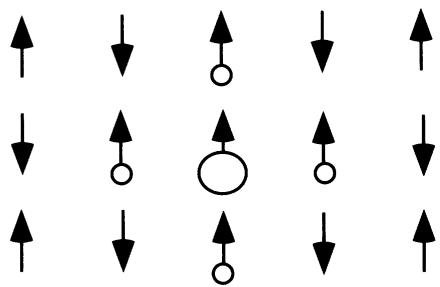
\includegraphics[width=0.45\textwidth]{fig19_1.jpg}
\caption{五格点极化子。圆圈描绘空穴密度。}
\label{fig:19.1}
\end{figure}

空穴的费米子谱有约 $2\bar{t}$ 的能隙。典型的自旋频率为

\begin{equation*}
\omega \sim \mathcal {O} ( \bar {J} S ^ {- 1} ) \ll \mathcal {O} ( \bar {t} ) ,
\tag{19.36}
\end{equation*}

因此空穴自由能的绝热近似是合理的。这与 Born--Oppenheimer 近似类似：慢自旋像重原子核，空穴像快电子，为慢变量确定一个有效势。

以格点 $i$ 为心的五格点极化子的自旋--空穴波函数为

\begin{equation*}
\left| \hat {\Omega} ^ {i}, \rho \right\rangle = \sum_{j = i, \, \langle ij \rangle} \sqrt {\rho_{j} [ \hat {\Omega} ^ {i} ]} \left| \hat {\Omega}_{j} ^ {i} \right\rangle_{S - \frac {1}{2}} f _ {j} ^ {\dagger} \left| 0 \right\rangle_{f _ {j}} \prod_{j ' \neq j} \left( \left| \hat {\Omega}_{j '} ^ {i} \right\rangle_{S} \left| 0 \right\rangle_{f _ {j '}} \right) ,
\tag{19.37}
\end{equation*}

$\rho[\hat{\Omega}^i]$ 是极化子组态 $\hat{\Omega}^i$ 的基态空穴密度。$S = \frac{1}{2}$ 时，(19.37) 可从纯 Néel 态 $\hat{\Omega}^N$ 通过

\begin{equation*}
\left| \hat {\Omega} ^ {i}, \rho \right\rangle = p _ {is _ {i}} ^ {\dagger} \left| \hat {\Omega} ^ {N} \right\rangle
\tag{19.38}
\end{equation*}

产生，$p^{\dagger}$ 是 Dagotto 与 Schrieffer 的准粒子算符

\begin{equation*}
p _ {is _ {i}} ^ {\dagger} \equiv \left( \sqrt {\rho_{i} [ \hat {\Omega} ^ {i} ]} + \sum_{\langle ij \rangle, s '} \sqrt {\rho_{j} [ \hat {\Omega} ^ {i} ]} \, c_{is '} ^ {\dagger} c_{js '} \right) c_{is}.
\tag{19.39}
\end{equation*}

$s_i = \pm \frac{1}{2}$ 是 $\hat{\Omega}_i^N$ 的自旋方向。

\section{极化子动力学与自旋隧穿}

五格点极化子破缺哈密顿量的自旋转动对称与格子平移对称。有限 $S$ 下，即使在零温，对称性也可由自旋的量子涨落恢复。恢复对称的涨落分两类：

\begin{enumerate}[itemsep=1pt]
\item 自旋波：倾向于恢复自旋对称，贡献在 $\mathcal{O}(1/S)$ 阶；
\item 自旋隧穿效应：移动极化子中心，恢复格子平移对称，是 $\mathcal{O}(e^{-S(\cdot)})$ 阶的非微扰效应。
\end{enumerate}

自旋波动力学可分别用第 11 章或第 12 章的方法处理有序相与无序相。

极化子的平移对称是分立的，自旋的任何运动都要爬越能垒。不过格子对称可以通过隧穿事件恢复：极化子的中心自旋转动到与近邻反铁磁关联，同时另一处的自旋转动形成新的五格点铁磁极化子（见图~\ref{fig:19.2}）。极化子从格点 $i$ 运动到 $k$ 的半经典隧穿矩阵元为\footnote{正确的多维隧穿矩阵元涉及受限制的波函数与磁通算符（见 Auerbach 与 Kivelson）。它们给出正确的前置因子 $\Gamma_{0}$，而 (19.40) 可用于领头阶行为。}

\begin{align*}
\Gamma_{ik} & \propto \left\langle \hat {\Omega} ^ {i} \left| G \left( E _ {0} ^ {cl} \right) \right| \hat {\Omega} ^ {k} \right\rangle\\
& = \int_{\hat {\Omega} ^ {i}} ^ {\hat {\Omega} ^ {k}} \mathcal {D} \hat {\Omega} ( t ) \, \exp \Bigg\{ i \int_ {0} ^ {\infty} d t \Big[ \sum_ {i} \left( S - \rho_{i} /2 \right) \left( 1 - \cos \theta_ {i} \right) \dot {\phi} _ {i}\\
& \quad \left. - \left( \bar {H} ^ {J} + E ^ {f} - E _ {0} ^ {cl} \right) \Big] \right\} ,
\tag{19.40}
\end{align*}

$G(E)$ 是 (10.38) 定义的依赖能量的 Green 函数。由转动对称，$H[\hat{\Omega}]$ 在所有方位角的统一平移

\begin{equation*}
\phi _ {i} = \bar {\phi} + \phi _ {i} '
\tag{19.41}
\end{equation*}

下不变。对动能项分部积分：

\begin{align*}
& \int \mathcal {D} \bar {\phi} ( t ) \exp \left[ - i \int d t \, \bar {\phi} ( t ) \, \partial_ {t} \left( \sum_ {i} \left[ S - \rho_{i} /2 ( t ) \right] \left[ 1 - \cos \theta_ {i} ( t ) \right] \right) \right]\\
& \propto \delta \left( M ^ {z} [ \hat {\Omega} ^ {i} ] - M ^ {z} [ \hat {\Omega} ^ {k} ] \right) ,
\tag{19.42}
\end{align*}

其中

\begin{equation*}
M ^ {z} [ \hat {\Omega} ( t ) ] = \sum_ {j} \left[ S - \rho_{j} ( t ) /2 \right] \left[ 1 - \cos \theta_ {j} ( t ) \right] = M ^ {z} [ \hat {\Omega} ( 0 ) ].
\tag{19.43}
\end{equation*}

也就是说，$z$ 磁化对 $G(E)$ 的任何矩阵元守恒。当然，这是哈密顿量转动不变性的精确推论。

一个重要结论是：在长程有序相中，五格点极化子不能在子晶格 A、B 之间隧穿，因为那会改变总磁化。换言之，存在一个禁止极化子跨子晶格跳跃的选择定则。这一强结果有些出人意料，因为原 t--J 哈密顿量 (19.27) 有大的跨子晶格跳跃项。物理上，原来的 $f$ 空穴被牢牢束缚于局域自旋缺陷，把低能下的电荷可动性限制在子晶格内的跳跃上。但要注意：若两个相距很远的格点所在处的局域环境具有反转的 Néel 场，极化子可以在分属相反子晶格的这两点之间隧穿（例如 Skyrmion 组态的中心与尾部）。

\begin{figure}[H]
\centering
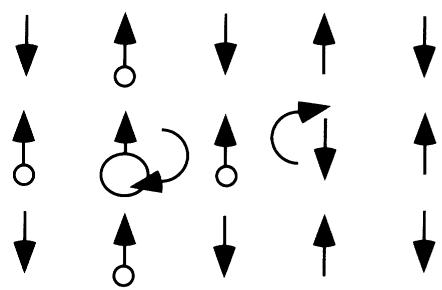
\includegraphics[width=0.45\textwidth]{fig19_2.jpg}
\caption{极化子的隧穿路径。}
\label{fig:19.2}
\end{figure}

隧穿路径是 (19.40) 的鞍点，连接 $\hat{\Omega}^i\to \hat{\Omega}^k$ 并满足变分运动方程

\begin{equation*}
\frac {\delta}{\delta \hat {\Omega} _ {i} ( \tau )} \int_ {0} ^ {\infty} d \tau ' \left[ \left( S - \rho_{i} /2 \right) \left( 1 - \cos \theta_ {i} \right) \dot {\phi} _ {i} - E ^ {cl} [ \hat {\Omega} ] \right] = 0.
\tag{19.44}
\end{equation*}

（我们已固定 $\mathbf{A}$ 的规范选择来进行隧穿率计算。）

确定隧穿路径至少可以用两条守恒规则：

\begin{enumerate}[itemsep=1pt]
\item 沿经典路径能量守恒（见 (10.37)）：

\begin{equation*}
E ^ {cl} [ \hat {\Omega}^{\mathrm{tun}} ( \tau ) ] = E _ {0} ^ {cl}.
\tag{19.45}
\end{equation*}

\item 总磁化守恒 (19.43)。
\end{enumerate}

由于 $\hat{\Omega}^{\mathrm{tun}}$ 穿越经典禁戒区域，只有把坐标复化才能找到解\footnote{自旋路径积分类似相空间路径积分，共轭变量是 $\cos\theta, \phi$，见 (11.7) 与 (11.5)。允许 $\phi$ 变虚等价于让动量变虚，即把时间延拓到 Feynman 路径积分的虚轴。}。设自旋沿 $\pm\hat{y}$ 方向有序，用 $\{\hat{\Omega}_{i}^{\mathrm{tun}}(\varphi)\}$ 参数化隧穿路径，$\varphi$ 是自旋 $i$ 的方位转动角。

把隧穿路径的 $\phi$ 变量复化：

\begin{equation*}
\phi ( \varphi ) \rightarrow \phi^ {\mathrm{re}} ( \varphi ) + i \phi^ {\mathrm{im}} ( \varphi ).
\tag{19.46}
\end{equation*}

用 (19.45)，(19.40) 的领头阶最陡下降近似为

\begin{align*}
\Gamma_{ik} & \approx - \sum_{\alpha} \Gamma_{0}^{\alpha} \exp \left( - W_{ik}^{\alpha} + i \Upsilon_{ik}^{\alpha} \right) ,\\
W_{ik} & = \int d \varphi \sum_{j} \frac {d \phi_{j}^{\mathrm{im}}}{d \varphi} \left( S - \rho_{j} /2 \right) \left( 1 - \cos \theta_{j} \right) ,\\
\Upsilon_{ik}^{\alpha} & = \int d \varphi \sum_{j} \frac {d \phi_{j}^{\mathrm{re}}}{d \varphi} \left( S - \rho_{j} /2 \right) \left( 1 - \cos \theta_{j} \right) ,
\tag{19.47}
\end{align*}

$\alpha$ 标记隧穿路径；$\Gamma_{0}^{\alpha}$ 是正的前置因子；整体负号是时间反演不变哈密顿量中简并极小之间隧穿矩阵元的一般特征。

由 (19.47) 可得一些定性信息。第一，$|\Gamma_{ik}|$ 随 $S$ 指数减小。第二，$\Gamma$ 的符号由 $\Upsilon$——一个 Berry 相位——决定。现在来确定五格点极化子隧穿的 $\Upsilon$。

由 $\phi_{i}\rightarrow-\phi_{i}$ 下的对称性，存在两条隧穿路径 $\hat{\Omega}^{\mathrm{tun},+}$ 与 $\hat{\Omega}^{\mathrm{tun},-}$，分别对应 $xy$ 平面内的顺时针与逆时针转动：

\begin{equation*}
\phi_{i}^{\mathrm{re}, +} ( \varphi ) = - \phi_{i}^{\mathrm{re}, -} ( \varphi ).
\tag{19.48}
\end{equation*}

于是两条路径有相同的 $W_{ik}$ 但相反的相位 $\Upsilon$。对两条路径求和：

\begin{align*}
\Gamma_{ik} \approx & - \Gamma_{0} \exp \left[ - \int_ {0} ^ {\pi} d \varphi \sum_{i} \left( S - \frac {\rho_{i}}{2} \right) \left( 1 - \cos \theta_{i} \right) \frac {d \phi_{i}^{\mathrm{im}}}{d \varphi} \right]\\
& \times \sum_{\pm} \exp \left[ i \int_ {0} ^ {\pm \pi} d \varphi \sum_{i} \left( S - \frac {\rho_{i}}{2} \right) \left( 1 - \cos \theta_{i} \right) \frac {d \phi_{i}^{\mathrm{re}}}{d \varphi} \right]\\
= & - 2 e ^ {i 2 \pi S} \left| \Gamma_{ik} \right| ,
\tag{19.49}
\end{align*}

其中

\begin{align*}
\left| \Gamma_{ik} \right| & = - \Gamma_{0} \cos \left( \int_ {0} ^ {\pm \pi} d \varphi \sum_{i} \frac {\rho_{i}}{2} \frac {d \phi_{i}^{\mathrm{re}}}{d \varphi} \right)\\
& \quad \times \exp \left[ - \int_ {0} ^ {\pi} d \varphi \sum_{i} \left( S - \frac {\rho_{i}}{2} \right) \left( 1 - \cos \theta_{i} \right) \frac {d \phi_{i}^{\mathrm{im}}}{d \varphi} \right] .
\tag{19.50}
\end{align*}

利用 $\sum_{i}\rho_{i}=1$ 可确立因子 $\cos(\int d\varphi\ldots)$ 为正。相位 $2\pi S$ 来自 $\phi_{i}$ 与 $\phi_{k}$ 的整体转动；其他自旋折返原路径，其 Berry 相位或为零、或与对称伙伴干涉相消。

在 (19.49) 中我们发现：对半奇整数自旋，极化子跳跃的符号为正。这影响基态动量如下。

设完美的 Néel 背景。极化子跳跃的能带结构为

\begin{align*}
\epsilon_{\mathbf {k}} & = \sum_ {j} \Gamma_{ij} \exp \left[ i \mathbf {k} \left( \mathbf {x} _ {i} - \mathbf {x} _ {j} \right) \right]\\
& \approx 2 \Gamma_{(2, 0)} \left[ \cos \left( 2 k _ {x} \right) + \cos \left( 2 k _ {y} \right) \right]\\
& \quad + 2 \Gamma_{(1, 1)} \left[ \cos \left( k _ {x} + k _ {y} \right) + \cos \left( k _ {x} - k _ {y} \right) \right] ,
\tag{19.51}
\end{align*}

$(1,1)$、$(2,0)$ 表示同一子晶格上的第一、第二近邻格点（见图~\ref{fig:19.3}）。更远程的跳跃隧穿率更小，忽略之。由 (19.49)，整数自旋（$\Gamma < 0$）时 $\epsilon_{k}$ 在 $k = 0$ 极小。半奇整数自旋时，基态动量位于线

\begin{equation*}
\mathbf {k} _ {0} \in \left\{ \mathbf {k} : \cos k _ {x} + \cos k _ {y} = 0 \right\}.
\tag{19.52}
\end{equation*}

$\Gamma_{ij}$ 的符号之所以重要，是因为子晶格内跳跃涉及三角形（见图~\ref{fig:19.3}），其负号无法通过重定义波函数或在 (19.44) 中选不同规范约定而“规范掉”。

半经典理论解释了小团簇上自旋 1/2 t--J 模型的数值研究\footnote{见 Dagotto 与 Schrieffer。}。第一，基态动量位于 $(0,\pi)$ 或 $(\pi/2,\pi/2)$（及其对称反演），与 (19.52) 一致。第二，准粒子权重因子

\begin{figure}[H]
\centering
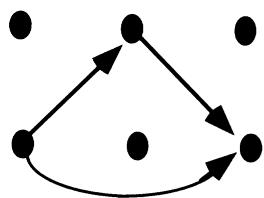
\includegraphics[width=0.45\textwidth]{fig19_3.jpg}
\caption{主导的极化子跳跃路径。}
\label{fig:19.3}
\end{figure}

\begin{equation*}
Z _ {h} = \left| \left\langle \Psi_ {0} ^ {t - J} \left| p_{\mathbf {k} _ {0} s} ^ {\dagger} \right| \Psi_ {0} ^ {\mathrm{Heis}} \right\rangle \right| ^ {2} / \left\langle \Psi_ {0} ^ {t - J} \left| p_{\mathbf {k} _ {0} s} p_{\mathbf {k} _ {0} s} ^ {\dagger} \right| \Psi_ {0} ^ {\mathrm{Heis}} \right\rangle
\tag{19.53}
\end{equation*}

可在小格子上测量。这里

\begin{equation*}
p _ {\mathbf {k} s} ^ {\dagger} = \sum_ {i} e ^ {- i \mathbf {k} \cdot \mathbf {x} _ {i}} p _ {is} ^ {\dagger}
\tag{19.54}
\end{equation*}

$p_{is}^{\dagger}$ 由 (19.39) 给出。$\Psi_{0}^{\mathrm{QHM}}, \Psi_{0}^{\mathrm{t-J}}$ 分别是 Heisenberg 模型与带一个空穴的 t--J 模型的精确基态。大 $S$ 极限下预期 $Z_{h} \rightarrow 1$。Dagotto 与 Schrieffer 数值计算了 $4 \times 4$ 正方格子 t--J 模型的 $Z_{h}$，在参数区 (19.34) 中发现

\begin{equation*}
0. 7 < Z _ {h} < 0. 94.
\tag{19.55}
\end{equation*}

这是 $S = \frac{1}{2}$ t--J 模型半经典近似的一次成功。差值 $1 - Z_{h}$ 度量五格点极化子短程关联的量子修正。

\section{$t^{\prime}$--$J$ 模型}

对多于一个空穴，经典基态由填充 $\bar{H}^{t}$ 的 $N^{f}$ 个最低态并极小化 (19.33) 的 $E^{cl}$ 得到。

19.3 节我们发现单极化子不诱导经典 Néel 态的长程畸变；且空穴密度局域于铁磁键附近，极化子之间的经典相互作用是短程的。但必须注意，量子涨落（自旋波）将在 $1/S$ 的更高阶引入更远程的相互作用。

对有限空穴密度，即 $\lim_{\mathcal{N}\to\infty}N^{f}/\mathcal{N}>0$，必须考虑相分离的可能性：体系可以通过把空穴挤进共享 Néel 背景畸变的区域来降低能量\footnote{见 Emery、Kivelson 与 Lin。}。

考虑到原 Hubbard 模型忽略了格点间排斥 Coulomb 相互作用，经典近似得到的短程力与相分离不稳定性在真实铜氧化物层中可能被压制。

然而，凭现有信息可以为极化子准粒子构造有效低能哈密顿量。把 (19.39) 中的 $|\hat{\Omega}^{N}\rangle$ 换成缓变的反铁磁关联组态，计算极化子跳跃率：

\begin{equation*}
\Gamma_{ik} \approx \delta_{s _ {i}, s _ {k}} \left\langle \hat {\Omega} ^ {i} \middle| \bar {\Omega} ^ {i} \right\rangle \bar {\Gamma} _ {ik} \left\langle \bar {\Omega} ^ {k} \middle| \hat {\Omega} ^ {k} \right\rangle ,
\tag{19.56}
\end{equation*}

$\bar{\Gamma}_{ik}$ 是 (19.49) 给出的未微扰隧穿率。$\bar{\Omega}^{i}$ 与 $\bar{\Omega}^{k}$ 表示平移到 $i$、$k$ 为心的五格点极化子，其自旋严格平行于一个共同方向——该方向分别使其与 $\hat{\Omega}^{i}$、$\hat{\Omega}^{k}$ 的交叠最大。(19.56) 中两个交叠因子的相位对每个自旋相消，除非 $\hat{\Omega}^{k}$ 与 $\hat{\Omega}^{i}$ 之间空穴密度不同。用 (19.37)：

\begin{align*}
\langle \hat {\Omega} ^ {i} | \bar {\Omega} ^ {i} \rangle \langle \bar {\Omega} ^ {k} | \hat {\Omega} ^ {k} \rangle & \approx \exp \left[ \frac {i}{2} \sum_ {j} \left( 2S - \rho_{j} ^ {i} \right) \cos \bar {\theta}_{j} ^ {i} \left( \phi_{j} ^ {i} - \bar {\phi}_{j} ^ {i} \right) \right]\\
& \quad \times \exp \left[ - \frac {i}{2} \sum_ {j} \left( 2S - \rho_{j} ^ {k} \right) \cos \bar {\theta}_{j} ^ {k} \left( \phi_{j} ^ {k} - \bar {\phi}_{j} ^ {k} \right) \right]\\
& = \exp \left[ - \frac {i}{2} \cos \bar {\theta} \left( \phi_{i} ^ {i} - \phi_{k} ^ {k} \right) \right] ,
\tag{19.57}
\end{align*}

这里用了一个极化子内总空穴密度为 1 的事实。Néel 规范场 $A^{N}$ 的格子定义已由 (17.11) 给出。这里我们发现极化子跳跃以规范协变方式\footnote{见 Shankar。}耦合到 Néel 规范场：

\begin{equation*}
\Gamma_{ik} = \bar {\Gamma}_{ik} \exp \left( i \eta_{i} \sum_{\mu} A^{N} \cdot \mathbf {x}_{ik} \right) ,
\tag{19.58}
\end{equation*}

$\eta_{i}=\mathrm{sign}(s_{i})$ 是极化子的有效“电荷”，依赖其子晶格指标。

(19.39) 的极化子算符 $p_{i}^{\dagger}$ 在大于两个晶格常量的距离上反对易。于是，长程有序相中稀疏极化子体系的低能性质由

\begin{equation*}
Z \propto \int \mathcal {D} \hat {\Omega} \, \mathcal {D} ^ {2} p \, \exp \left( \int_ {0} ^ {\beta} i \sum_ {i} 2S \mathbf {A} \cdot \dot {\hat {\Omega}} _ {i} - \frac {\bar {J}}{4} \sum_{\langle ij \rangle} \hat {\Omega} _ {i} \cdot \hat {\Omega} _ {j} - L ^ {p} \right)
\tag{19.59}
\end{equation*}

描述，$L^{p}$ 是无自旋 Grassmann 变量 $p_{i}$ 的 Lagrange 量：

\begin{align*}
L ^ {p} & = \sum_ {i} p _ {i} ^ {*} \left( \partial_ {\tau} + i \eta_ {i} A _ {0} ^ {N} + \mu \right) p _ {i} + \sum_{\langle i, j, k \rangle} \Gamma_{ik} e ^ {i \eta_{i} \mathbf {A}^{N} \cdot \mathbf {x}_{ik}} p _ {i} ^ {\dagger} p _ {k}\\
& \quad + \sum_ {ij} U _ {ij} p _ {i} ^ {*} p _ {i} p _ {j} ^ {*} p _ {j} .
\tag{19.60}
\end{align*}

$U_{ij}$ 是双极化子有效相互作用。$L^{p}$ 的规范不变性反映 (19.18) 所示自旋与电荷的局域约束。用满足 (19.10) 的有效从属费米子与 Schwinger 玻色子算符近似极化子与自旋自由度，与 (19.60) 对应的最小哈密顿量是 $t^{\prime}$--$J$ 模型：

\begin{equation*}
\mathcal {H} ^ {t ' - J, s} = P _ {s} \left[ \bar {J} \sum_{\langle ij \rangle} \mathbf {S} _ {i} \cdot \mathbf {S} _ {j} + \sum_{\langle i, k \rangle} \Gamma_{ik} \, p_{i} ^ {\dagger} p_{k} \left( a_{i} ^ {\dagger} a_{k} + b_{i} ^ {\dagger} b_{k} \right) \right] P _ {s} ,
\tag{19.61}
\end{equation*}

自旋 1/2 时：

\begin{equation*}
\mathcal {H} ^ {t ' - J} = P _ {s} \left( \bar {J} \sum_{\langle ij \rangle} \mathbf {S} _ {i} \cdot \mathbf {S} _ {j} - \sum_{\langle i, k \rangle, s} \Gamma_{ik} \, c _ {is} ^ {\dagger} c _ {ks} \right) P _ {s}.
\tag{19.62}
\end{equation*}

$c_{is}$ 是电子算符。$t^{\prime}$--$J$ 模型与初始 t--J 模型的差别在于没有跨子晶格跳跃。$t'$ 跳跃与自旋的局域相互作用较弱，因为空穴在同一子晶格上跳跃时不留下一串反转的自旋。这使得 $t^{\prime}$--$J$ 模型的跳跃项更适于弱耦合处理——至少在反铁磁相中如此。此外，如下文所述，可以用连续近似描述低空穴浓度的低能动力学。

\subsection{超导电性？}

循 Haldane 映射\footnote{见第 12 章。}，自旋相互作用由 $(2+1)$ 维非线性 {$\sigma$} 模型描述，劲度常数与自旋波速度依赖浓度。预期在某个临界密度之上长程自旋序消失，但反铁磁关联在短长度尺度上存留。如 (19.60) 所示，低能自旋涨落通过 Néel 规范场与极化子耦合。Wiegmann、Wen、Shankar 与 Lee（WWSL）为这一耦合体系提出了一个有效场论：

\begin{equation*}
\mathcal {L}^{\mathrm{WWSL}} = \sum_{\alpha = A, B} L^{p, \alpha} [ - i \partial_{\mu} + \eta_{\alpha} A_{\mu}^{N} ] + \frac {1}{m^ {2}} \sum_{\mu \nu} \left( F_{\mu \nu} \right) ^ {2} ,
\tag{19.63}
\end{equation*}

$L^{p,\alpha}$ 是子晶格 $\alpha$ 上极化子的长波 Lagrange 量；手性自旋涨落由 Néel 规范场导出的“电磁场”描述：

\begin{equation*}
F _ {\nu \mu} = \partial_ {\mu} A _ {\nu} ^ {N} - \partial_ {\nu} A _ {\mu} ^ {N}.
\tag{19.64}
\end{equation*}

$m$ 是 Néel 规范场的有效耦合常数，粗略正比于逆自旋关联长度\footnote{见 A. M. Polyakov, \textit{Gauge Fields and Strings} (Harwood, 1987), 8.3 节。}。

WWSL 提出 (19.63) 的基态可能是高温超导体。基本论证是：不同子晶格上的极化子相对 Néel 规范场带相反电荷，在极化子之间产生类电磁吸引。这是一种运动学配对机制，对有效模型的短程相互作用不敏感。而且该方案在磁无序相中依然有效。这尤为令人满意，因为实验上铜氧化物超导体中反铁磁性与超导电性似乎并不共存。

\begin{exercises}

\item 设半径 $R_{c}$ 的大圆形区域内所有自旋铁磁关联。计算大 $\bar{t}/\bar{J}$ 的经典基态能量 $E^{cl}$，对 $R_{c}$ 极小化能量以证明 (19.35)。

\end{exercises}

\begin{chapbib}
\item t--J 模型的 Schwinger 玻色子平均场理论由
  C. Jayaprakash, H. R. Krishnamurthy, and S. Sarker, Phys. Rev. B \textbf{40}, 2610 (1989)；
  C. L. Kane, P. A. Lee, T. K. Ng, B. Chakraborty, and N. Read, Phys. Rev. B \textbf{41}, 2653 (1990)
  完成。
\item 经典极限下极化子大小与相互作用的计算见
  A. Auerbach and B. E. Larson, Phys. Rev. Lett. \textbf{66}, 2262 (1991)。
\item 空穴在涨落反铁磁背景中的规范耦合，最早在连续表述中导出于
  R. Shankar, Nucl. Phys. B \textbf{330}, 433 (1990)。
\item 用受限 Green 函数（“路径分解展开”）计算多维隧穿率的综述：
  A. Auerbach and S. Kivelson, Nucl. Phys. Rev. B \textbf{257}, 799 (1985)。
\item 极化子算符的定义及其权重在小格子上对 t--J 模型的数值计算：
  E. Dagotto and J. R. Schrieffer, Phys. Rev. B \textbf{43}, 8705 (1991)。
\item t--J 模型相分离的变分论证：
  V. J. Emery, S. A. Kivelson, and H. Q. Lin, Phys. Rev. Lett. \textbf{64}, 475 (1990)。
\item $t^{\prime}$--$J$ 模型高温超导理论由
  P. B. Wiegmann, Phys. Rev. Lett. \textbf{60}, 821 (1988)；
  P. A. Lee, Phys. Rev. Lett. \textbf{63}, 690 (1989)；
  X.-G. Wen, Phys. Rev. B \textbf{39}, 7223 (1989)
  提出。
\item 二维反铁磁体中空穴问题的其他途径：
  S. Trugman, Phys. Rev. B \textbf{41}, 892 (1990)；
  B. Schraiman and E. Siggia, Phys. Rev. Lett. \textbf{62}, 156 (1989)。
\end{chapbib}


% 第四部分 数学附录
\part{数学附录}
\vspace{2em}
\begin{center}
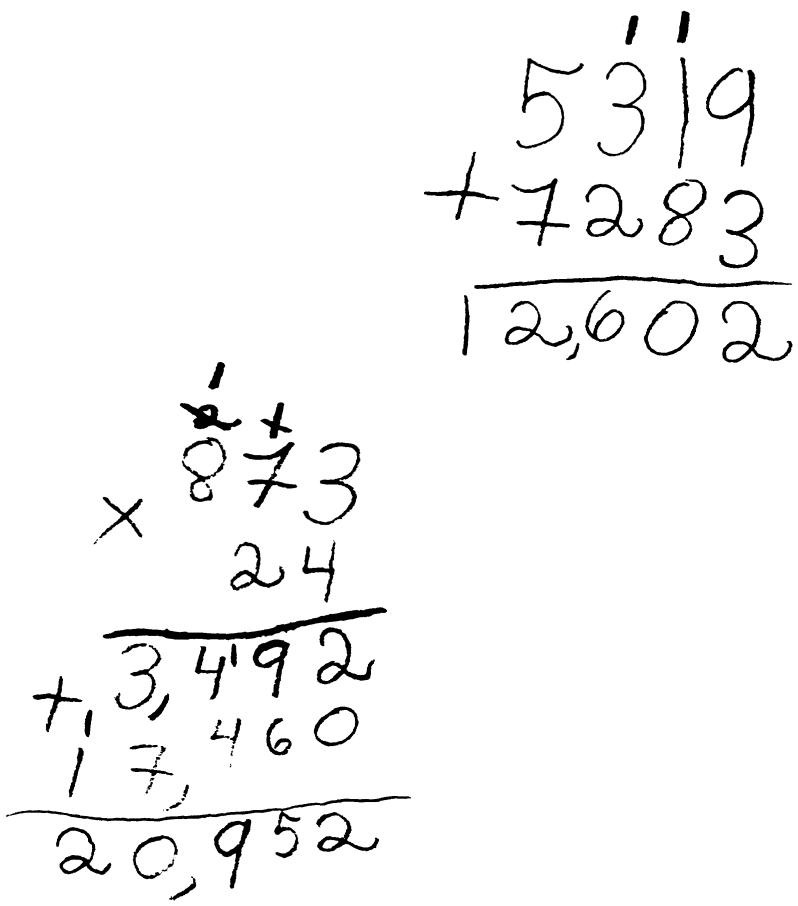
\includegraphics[width=0.5\textwidth]{deco_part4.jpg}

{\kaishu 插图：Dick Codor}
\end{center}

\appendix
\ctexset{chapter/name={附录,}}
% 附录A 第二次量子化
\chapter{第二次量子化}

这里复习正文中通用的二次量子化的标准定义与基本关系。

\section{Fock 态}

给定正交归一的单粒子基底 $\{|\phi_{i}\rangle\}_{i=1}^{N}$：

\begin{equation*}
\langle \phi_ {i} | \phi_ {j} \rangle = \delta_ {ij}.
\tag{A.1}
\end{equation*}

态 $i$ 的产生算符是 $a_{i}^{\dagger}$，其厄米共轭是湮灭算符 $a_{i}$。二者都相对真空态 $|0\rangle_{i}$ 定义：

\begin{equation*}
\left| \phi_ {i} \right\rangle = a _ {i} ^ {\dagger} \left| 0 \right\rangle_{i} \, , \quad a _ {i} \left| 0 \right\rangle_{i} = 0.
\tag{A.2}
\end{equation*}

数算符定义为

\begin{equation*}
n _ {i} \equiv a _ {i} ^ {\dagger} a _ {i}.
\tag{A.3}
\end{equation*}

利用对易规则

\begin{equation*}
\left[ a _ {i} ^ {\dagger} a _ {i}, \left( a _ {i} ^ {\dagger} \right) ^ {n} \right] = n \left( a _ {i} ^ {\dagger} \right) ^ {n} ,
\tag{A.4}
\end{equation*}

可以验证反复作用 $a_{i}^{\dagger}$（$a_{i}$）增加（减少）态 $\phi_{i}$ 中的粒子数。以占据数 $n_{i}$ 标记的 Fock 态定义为

\begin{equation*}
\left| n _ {1}, n _ {2}, \dots \right\rangle = \prod_ {i} \frac {\left( a _ {i} ^ {\dagger} \right) ^ {n _ {i}}}{\sqrt {n _ {i} !}} \left| 0 \right\rangle_{i}.
\tag{A.5}
\end{equation*}

对多玻色子（或费米子），Fock 态的对称（反对称）性由对易（反对易）关系强制：

\begin{equation*}
\left[ a _ {i}, a _ {j} ^ {\dagger} \right]_{\eta} = a _ {i} a _ {j} ^ {\dagger} - \eta \, a _ {j} ^ {\dagger} a _ {i} = \delta_{ij} ,
\tag{A.6}
\end{equation*}

\begin{equation*}
\left[ a _ {i}, a _ {j} \right]_{\eta} = 0 ,
\tag{A.7}
\end{equation*}

其中

\begin{equation*}
\eta = \left\{ \begin{array}{ll} 1 & \text{玻色子} \\ - 1 & \text{费米子} \end{array} \right.
\tag{A.8}
\end{equation*}

占据数受总粒子数约束限制：

\begin{equation*}
\sum_ {i} n _ {i} = N.
\tag{A.9}
\end{equation*}

对易（反对易）关系定义了二次量子化算符的一个代数。该代数在二次量子化算符的正则变换下不变。这里只考虑正规（normal）变换\footnote{关于 Bogoliubov 变换的专著见文献注释。}。考虑单粒子基底上的幺正变换 $U$：

\begin{equation*}
a _ {\alpha} ^ {\dagger} = \sum_ {i} U _ {\alpha i} a _ {i} ^ {\dagger} \, , \quad U ^ {\dagger} U = I.
\tag{A.10}
\end{equation*}

容易验证 $\{a_{\alpha}^{\dagger}\}$ 与 $\{a_{\alpha}\}$ 满足正则代数 (A.6) 与 (A.7)。

\section{正规双线性算符}

双线性算符由

\begin{equation*}
\hat {A} = \sum_ {ij} a _ {i} ^ {\dagger} A _ {ij} a _ {j} \equiv \mathbf {a} ^ {\dagger} \cdot A \cdot \mathbf {a}
\tag{A.11}
\end{equation*}

给出，$A$ 是基底 $\phi_{i}$ 中的厄米矩阵，即单粒子算符。

玻色子或费米子的双线性算符与线性算符的对易关系特别简单。矢量 $\mathbf{v}$ 定义线性算符 $\hat{v}^{\dagger}$：

\begin{equation*}
\hat {\mathbf {v}} ^ {\dagger} = \sum_ {i} v _ {i} a _ {i} ^ {\dagger} = \mathbf {v} \cdot \mathbf {a} ^ {\dagger}.
\tag{A.12}
\end{equation*}

把 (A.11) 与 (A.12) 对易：

\begin{equation*}
\left[ \hat {A}, \hat {\mathbf {v}} ^ {\dagger} \right] = \left( A \mathbf {v} \right) \cdot \mathbf {a} ^ {\dagger}.
\tag{A.13}
\end{equation*}

若 $\mathbf{v}$ 是 $A$ 的本征值为 $v$ 的本征矢量，则 $\hat{v}^{\dagger}$ 是 $[A,\cdot]$ 的本征值为 $v$ 的本征算符。这可用于计算 $\hat{v}^{\dagger}$ 在转动下的变换：

\begin{align*}
e ^ {i\theta \hat {A}} \hat {\mathbf {v}} ^ {\dagger} e ^ {-i\theta \hat {A}} & = \hat {\mathbf {v}} ^ {\dagger} + i\theta \left[ \hat {A}, \hat {\mathbf {v}} ^ {\dagger} \right] + \frac {( i\theta ) ^ {2}}{2} \left[ \hat {A}, \left[ \hat {A}, \hat {\mathbf {v}} ^ {\dagger} \right] \right] + \dots\\
& = e ^ {iv\theta} \hat {\mathbf {v}} ^ {\dagger} .
\tag{A.14}
\end{align*}

幺正矩阵 $U$ 可用一组厄米生成元 $A_{\alpha}$ 与参数 $\theta_{\alpha}$ 写出：

\begin{equation*}
U _ {\theta} = e ^ {i \sum_ {\alpha} \theta_{\alpha} A_{\alpha}}.
\tag{A.15}
\end{equation*}

相应的多粒子算符 $\hat{U}$ 定义为

\begin{equation*}
\hat {U} _ {\theta} = e ^ {i \sum_ {\alpha} \theta_{\alpha} \hat {A}_{\alpha}}.
\tag{A.16}
\end{equation*}

利用 (A.14)，容易证明 $\hat{\mathbf{v}}^{\dagger}$ 在 $\hat{U}$ 下按简单方式变换：

\begin{equation*}
\hat {U} _ {\theta} \hat {\mathbf {v}} ^ {\dagger} \hat {U} _ {\theta} ^ {- 1} = \left( U _ {\theta} \mathbf {v} \right) \cdot \mathbf {a} ^ {\dagger}.
\tag{A.17}
\end{equation*}

两个双线性算符之间的对易关系是

\begin{equation*}
\left[ \hat {A}, \hat {B} \right] = \mathbf {a} ^ {\dagger} [ A, B ] \mathbf {a}.
\tag{A.18}
\end{equation*}

(A.17) 与 (A.18) 对费米子与玻色子都成立。

\subsection*{例：自旋代数}

双线性自旋算符是

\begin{equation*}
S ^ {\alpha} = \frac {1}{2} \sum_{ss' = 1} ^ {2} a _ {s} ^ {\dagger} \sigma_{ss'} ^ {\alpha} a _ {s '} \, , \quad \alpha = x, y, z ,
\tag{A.19}
\end{equation*}

其中

\begin{equation*}
\left( \sigma^ {x}, \sigma^ {y}, \sigma^ {z} \right) = \left[ \left( \begin{array}{cc} 0 & 1 \\ 1 & 0 \end{array} \right) , \left( \begin{array}{cc} 0 & -i \\ i & 0 \end{array} \right) , \left( \begin{array}{cc} 1 & 0 \\ 0 & -1 \end{array} \right) \right].
\tag{A.20}
\end{equation*}

计算 Pauli 矩阵的对易关系并用 (A.18)，可以验证 $S^{\alpha}$ 满足角动量关系

\begin{equation*}
\left[ S ^ {\alpha}, S ^ {\beta} \right] = i \epsilon^ {\alpha \beta \gamma} S ^ {\gamma} ,
\tag{A.21}
\end{equation*}

$\epsilon$ 是全反对称张量。

\section{无相互作用哈密顿量}

正规二次型哈密顿量为

\begin{equation*}
\mathcal {H} = \sum_ {ii '} a _ {i} ^ {\dagger} H _ {ii '} a _ {i '} = \sum_ {k} \left( \epsilon_ {k} - \mu \right) a _ {k} ^ {\dagger} a _ {k} ,
\tag{A.22}
\end{equation*}

$H$ 厄米，$\epsilon_{k}, a_{k}$ 分别是它的能量与本征算符，$\mu$ 是化学势。配分函数为

\begin{align*}
Z & = \operatorname{Tr} e ^ {- \mathcal {H} /T} = \prod_ {k} \sum_{n _ {k} = 0} ^ {n_{\mathrm{max}}} \exp \left[ - \frac {\left( \epsilon_ {k} - \mu \right) n _ {k}}{T} \right]\\
& = \prod_ {k} \left( 1 - \eta \, e ^ {- \left( \epsilon_ {k} - \mu \right) /T} \right) ^ {- \eta} .
\tag{A.23}
\end{align*}

(A.23) 中 $n_{\mathrm{max}}$ 对玻色子为无穷，对费米子为 1。

由 (A.23)，自由能为

\begin{equation*}
F \equiv -T \ln Z = \eta T \sum_ {k} \ln \left( 1 - \eta \, e ^ {- \left( \epsilon_ {k} - \mu \right) /T} \right).
\tag{A.24}
\end{equation*}

平衡占据概率为

\begin{align*}
\langle n _ {k} \rangle & = \frac {1}{Z} \operatorname{Tr} \left[ a _ {k} ^ {\dagger} a _ {k} e ^ {- H /T} \right] = \frac {\partial F}{\partial \epsilon_ {k}}\\
& = \left( e ^ {\left( \epsilon_ {k} - \mu \right) /T} - \eta \right) ^ {- 1} ,
\tag{A.25}
\end{align*}

$\eta = \pm1$ 时分别是 Bose 函数与 Fermi 函数。

\begin{exercises}

\item 两个 $N$ 费米子 Fock 态 $\Phi_1 = |\{n_i\} \rangle$ 与 $\Phi_2 = |\{n_\alpha\} \rangle$ 分别相对基底 $\{\phi_i\}$ 与 $\{\phi_\alpha\}$ 定义，两基底由幺正矩阵 $U$ 联系：

\begin{equation*}
\phi_ {\alpha} = \sum_ {i} U _ {\alpha i} \phi _ {i}.
\tag{A.26}
\end{equation*}

用矩阵 $U$ 表出交叠 $\langle\Phi_{1}|\Phi_{2}\rangle$。

\item 自旋转动算符为

\begin{equation*}
R = \exp \left[ iS ^ {z} \phi \right] \exp \left[ iS ^ {y} \theta \right] \exp \left[ iS ^ {z} \chi \right].
\tag{A.27}
\end{equation*}

注意 $R$ 是定义在费米子 Fock（占据数）空间中的算符。用 (A.17)，求 $SU(2)$ 变换矩阵 $U_{ss'}$ 的显式表达式：

\begin{equation*}
\left( c ' \right)_{s} = \left( R c R ^ {- 1} \right)_{s} = \sum_ {s '} U _ {ss'} \left( \phi, \theta, \chi \right) c _ {s '}.
\tag{A.28}
\end{equation*}

\item 求双线性形式

\begin{equation*}
c _ {1 \uparrow} ^ {\dagger} c _ {2 \downarrow} ^ {\dagger} - c _ {1 \downarrow} ^ {\dagger} c _ {2 \uparrow} ^ {\dagger}
\tag{A.29}
\end{equation*}

在整体自旋转动下的变换，其中 $c_{1s}$ 与 $c_{2s}$ 代表两个不同轨道上的电子。

\item 证明：对 (A.28) 给出的任何整体转动，顺磁 Fermi 气体态保持不变：

\begin{equation*}
\prod_{s, \, | k | < \pi / 2} \left( c _ {ks} ^ {\dagger} \right) ' \left| 0 \right\rangle = \prod_{s, \, | k | < \pi / 2} c _ {ks} ^ {\dagger} \left| 0 \right\rangle .
\tag{A.30}
\end{equation*}

\end{exercises}

\begin{chapbib}
\item 广义 Bogoliubov 变换的讨论见
  R. Balian and E. Brézin, Nuovo Cimento B \textbf{LXIV}, 37 (1969)。
\end{chapbib}

% 附录B 线性响应与生成泛函
\chapter{线性响应与生成泛函}

\section{自旋响应函数}

自旋响应函数描述自旋对任意弱的、依赖时空的磁场（或“源流”）$j_{i}^{\alpha}(t)$（$t \geq 0$ 时开启）的响应动力学。完整的依赖源的哈密顿量为

\begin{equation*}
\mathcal {H} [ j ] = \mathcal {H} _ {0} - \sum_ {\mathbf {q}} j _ {i} ^ {\alpha} ( t ) S _ {i} ^ {\alpha} ,
\tag{B.1}
\end{equation*}

$\alpha = x, y, z$。$t > 0$ 时 Hilbert 空间中所有态按 Schrödinger 方程演化：

\begin{equation*}
i \frac {\partial}{\partial t} \left| \psi ( t ) \right\rangle = \mathcal {H} [ j ] \left| \psi ( t ) \right\rangle .
\tag{B.2}
\end{equation*}

(B.2) 的解由演化算符给出：

\begin{align*}
\left| \psi ( t ) \right\rangle & = U [ t, j ] \left| \psi ( 0 ) \right\rangle ,\\
U [ t, j ] & = T _ {t '} \exp \left( - i \int_ {0} ^ {t} d t ' \, \mathcal {H} [ j ( t ' ) ] \right) ,
\tag{B.3}
\end{align*}

$\mathcal{H}_{0}(\mu)$ 是巨正则表述中的无相互作用哈密顿量。时序指数定义为离散表达式的极限：

\begin{align*}
& T _ {t '} \exp \left[ - i \int_ {0} ^ {t} d t ' \, \mathcal {H} ( t ' ) \right]\\
= & \lim_{\epsilon \rightarrow 0} \underbrace {\left[ 1 - i \mathcal {H} ( t ) \epsilon \right] \left[ 1 - i \mathcal {H} ( t - 2\epsilon ) \epsilon \right] \dots \left[ 1 - i \mathcal {H} ( \epsilon ) \epsilon \right]}_{N _ {\epsilon}} ,
\tag{B.4}
\end{align*}

$\epsilon = t / N_{\epsilon}$ 是无穷小时间步长。

算符 $S_{i}^{\alpha}$ 的期望值在 $\mathcal{H}[j]$ 下演化为

\begin{equation*}
\langle S _ {i} ^ {\alpha} ( t ) \rangle_{j} = Z ^ {- 1} \operatorname{Tr} \left( \rho \, U ^ {- 1} [ t, j ] \, S _ {i} ^ {\alpha} \, U [ t, j ] \right) ,
\tag{B.5}
\end{equation*}

$Z = \operatorname{Tr}\rho$ 是配分函数，$\rho$ 是密度矩阵。到源流 $j$ 的线性阶，(B.5) 给出

\begin{equation*}
\langle S _ {i} ^ {\alpha} ( t ) \rangle_{j} = \langle S _ {i} ^ {\alpha} ( 0 ) \rangle + i \int_ {0} ^ {t} d t ' \sum_{i ', \alpha '} j_{i '} ^ {\alpha '} \left\langle \left[ S _ {i} ^ {\alpha} ( t ), S _ {i '} ^ {\alpha '} ( t ' ) \right] \right\rangle + \mathcal {O} ( j ^ {2} ) ,
\tag{B.6}
\end{equation*}

$\langle\cdot\rangle$ 相对 $H_{0}$ 定义。(B.6) 中积分的核就是响应函数

\begin{equation*}
R_{ii'} ^ {\alpha \alpha'} ( t - t ' ) = - i \theta ( t - t ' ) \left\langle \left[ S _ {i} ^ {\alpha} ( t ), S _ {i'} ^ {\alpha} ( t ' ) \right] \right\rangle .
\tag{B.7}
\end{equation*}

由于 $\theta$ 函数，$R$ 也称为“推迟”关联函数。

可以用 $\mathcal{H}_0$ 的本征态与本征能量计算 $R$：

\begin{equation*}
\mathcal {H} _ {0} ( \mu ) \left| n \right\rangle = E _ {n} \left| n \right\rangle .
\tag{B.8}
\end{equation*}

在本征态表示中，(B.7) 为

\begin{align*}
R_{ii'} ( t ) & = - i \theta ( t ) Z ^ {- 1} \sum_{nm} e ^ {- E_{n} /T} \Big( e ^ {i ( E_{n} - E_{m} ) t} \langle n | S _ {i} ^ {\alpha} | m \rangle \langle m | S _ {i'} ^ {\alpha} | n \rangle\\
& \quad - e ^ {i ( E_{m} - E_{n} ) t} \langle n | S _ {i'} ^ {\alpha} | m \rangle \langle m | S _ {i} ^ {\alpha} | n \rangle \Big) .
\tag{B.9}
\end{align*}

哈密顿量的平移不变性给出 $R_{ii'} = R(\mathbf{x}_i - \mathbf{x}_{i'})$，$x_i$ 是格点 $i$ 的位置。$R$ 的时空 Fourier 变换为

\begin{align*}
R ( \mathbf {q}, \omega + i0 ^ {+} ) & = \mathcal {N} ^ {- 1} \sum_{ii'} \int_ {0} ^ {\infty} d t \, e ^ {- i \mathbf {q} ( \mathbf {x} _ {i} - \mathbf {x} _ {i'} ) + i ( \omega + i0 ^ {+} ) t} R ( \mathbf {x} _ {i} - \mathbf {x} _ {i'}, t )\\
& = ( \mathcal {N} Z ) ^ {- 1} \sum_{n, m} \langle n | S _ {\mathbf {q}} ^ {\alpha} | m \rangle \langle m | S _ {- \mathbf {q}} ^ {\alpha} | n \rangle \frac {e ^ {- E_{n} /T} - e ^ {- E_{m} /T}}{E _ {n} - E _ {m} + \omega + i0 ^ {+}} ,
\tag{B.10}
\end{align*}

其中

\begin{equation*}
S _ {\mathbf {q}} ^ {\alpha} = \sum_ {i} e ^ {- i \mathbf {qx} _ {i}} S _ {i} ^ {\alpha}.
\tag{B.11}
\end{equation*}

无穷小正数 $0^{+}$ 保证 Fourier 积分在大时间收敛。$R$ 的实部与虚部由恒等式

\begin{equation*}
\frac {1}{x + i0 ^ {+}} = \mathcal {P} \left( \frac {1}{x} \right) - i \pi \delta ( x )
\tag{B.12}
\end{equation*}

给出，$\mathcal{P}$ 取主值。把 (B.12) 用于 (B.10)，可以证明 Kramers--Kronig 关系：

\begin{align*}
\operatorname{Re} R ( \mathbf {q}, \omega ) & = \mathcal {P} \int_{- \infty} ^ {\infty} \frac {d \omega '}{\pi} \frac {\operatorname{Im} R ( \mathbf {q}, \omega ' )}{\omega ' - \omega} ,\\
\operatorname{Im} R ( \mathbf {q}, \omega ) & = - \mathcal {P} \int_{- \infty} ^ {\infty} \frac {d \omega '}{\pi} \frac {\operatorname{Re} R ( \mathbf {q}, \omega ' )}{\omega ' - \omega} .
\tag{B.13}
\end{align*}

\section{涨落与耗散}

谱响应函数的虚部 $\operatorname{Im} R_{21}(\omega)$ 是耗散部分，描述频率 $\omega$ 的外振荡通过激发体系内部模式而被阻尼。平衡时两个自旋涨落之间的关联函数是

\begin{equation*}
S_{i, i'} ^ {\alpha \alpha'} ( t - t ' ) = \left\langle S _ {i} ^ {\alpha} ( t ) \cdot S _ {i'} ^ {\alpha'} ( t ' ) \right\rangle .
\tag{B.14}
\end{equation*}

其 Fourier 变换称为动力学结构因子：

\begin{align*}
S ^ {\alpha \alpha'} ( \mathbf {q}, \omega ) & = \mathcal {N} ^ {- 1} \sum_{ii'} \int_{- \infty} ^ {\infty} d t \, e ^ {- i \mathbf {q} ( \mathbf {x} _ {i} - \mathbf {x} _ {i'} ) + i\omega t} S_{ii'} ^ {\alpha \alpha'} ( t )\\
& = \frac {2 \pi}{Z \mathcal {N}} \sum_{n, m} e ^ {- E_{n} /T} \langle n | S _ {\mathbf {q}} ^ {\alpha} | m \rangle \langle m | S _ {- \mathbf {q}} ^ {\alpha'} | n \rangle \, \delta \left( \omega + E_{n} - E_{m} \right) .
\tag{B.15}
\end{align*}

对厄米可观察量，结构因子 $S(\mathbf{q},\omega)$ 为实。它描述频率 $\omega$ 的自发涨落，可由散射实验测量。例如，极化的非弹性中子散射截面测量的正是电子自旋结构因子。

比较 (B.10) 与 (B.15) 的显式表达式，得到耗散响应函数与结构因子之间的简单关系（略去上标）：

\begin{equation*}
S ( \mathbf {q}, \omega ) = - \frac {2}{1 - e ^ {- \omega /T}} \operatorname{Im} R ( \mathbf {q}, \omega ).
\tag{B.16}
\end{equation*}

这一关系称为涨落--耗散定理。

\section{生成泛函}

理论家关心的是从微观模型计算响应函数或结构因子。使这类计算在相互作用多粒子体系中可行的有用工具是虚时生成泛函。正文中我们遇到过生成泛函的路径积分表示，它们适合作半经典或大 $N$ 近似。这里把响应函数 $R(\mathbf{q},\omega)$ 导出为生成泛函的二阶导数。

巨正则生成泛函定义为

\begin{equation*}
Z [ j, \mu ] = \operatorname{Tr} T _ {\tau} \left( \exp \left[ - \int_ {0} ^ {\beta} d \tau \, \mathcal {H} [ j ( \tau ) ] \right] \right) ,
\tag{B.17}
\end{equation*}

其中

\begin{equation*}
\mathcal {H} [ j ( \tau ) ] = \mathcal {H} _ {0} ( \mu ) - \sum_ {i} j _ {i} ^ {\alpha} ( \tau ) S _ {i} ^ {\alpha} \, , \quad \tau \in [ 0, \beta ).
\tag{B.18}
\end{equation*}

时序算符 $T(\bullet)$（先前在 (B.4) 中使用）把算符按 $\tau$ 从右到左递增排序。

对转动对称的 $H_{0}$，$\langle S_{i}^{\alpha}\rangle = 0$。虚时关联函数定义为

\begin{align*}
\tilde {R}_{i, i'} ^ {\alpha \alpha'} ( \tau, \tau ' ) & = \left. \frac {\delta^ {2} \ln Z}{\delta j_{i} ^ {\alpha} ( \tau ) \, \delta j_{i'} ^ {\alpha'} ( \tau ' )} \right| _ {j = 0}\\
& = Z ^ {- 1} \operatorname{Tr} \left\{ e ^ {- \beta \mathcal {H} _ {0}} T _ {\tau} \left[ S _ {i} ^ {\alpha} ( \tau ) S _ {i'} ^ {\alpha} ( \tau ' ) \right] \right\} ,
\tag{B.19}
\end{align*}

其中

\begin{equation*}
S _ {i} ^ {\alpha} ( \tau ) \equiv e ^ {\mathcal {H} _ {0} \tau} S _ {i} ^ {\alpha} e ^ {- \mathcal {H} _ {0} \tau} ,
\tag{B.20}
\end{equation*}

时序定义为

\begin{equation*}
T _ {\tau} \left[ A ( \tau ) B ( \tau ' ) \right] = \left\{ \begin{array}{ll} A ( \tau ) B ( \tau ' ) & \tau \geq \tau ' \\ B ( \tau ' ) A ( \tau ) & \tau < \tau ' \end{array} \right..
\tag{B.21}
\end{equation*}

由 (B.19)，利用迹的循环性质，验证

\begin{equation*}
\tilde {R} ( \tau, \tau ' ) = \tilde {R} ( \tau - \tau ', 0 ) \equiv \tilde {R} ( \tau - \tau ' )
\tag{B.22}
\end{equation*}

且 $\tilde{R} (\tau)$ 在区间 $[0,\beta)$ 上周期：

\begin{equation*}
\lim_{\tau \rightarrow \beta ^ {-}} \tilde {R} ( \tau ) = \lim_{\tau \rightarrow 0 ^ {-}} \tilde {R} ( \tau ).
\tag{B.23}
\end{equation*}

对时空平移不变的哈密顿量，用 $\tilde{R}_{ii'}(\tau)$ 的 Fourier 表示是方便的：

\begin{equation*}
\tilde {R} ( \mathbf {q}, i\omega_ {n} ) = \mathcal {N} ^ {- 1} \sum_{ii'} \int_ {0} ^ {\beta} d \tau \, e ^ {- i \mathbf {q} ( \mathbf {x} _ {i} - \mathbf {x} _ {i'} ) - i\omega_{n} \tau} \tilde {R}_{ii'} ( \tau ) ,
\tag{B.24}
\end{equation*}

\begin{equation*}
\omega_ {n} = 2 n \pi \beta^ {- 1} \, , \quad n = 0, \pm 1, \pm 2, \dots .
\tag{B.25}
\end{equation*}

频率 $\omega_{n}$ 是 Bose--Matsubara 频率。在 (B.19) 的算符之间插入完备本征态集并在 (B.24) 中完成 $d\tau$ 积分，发现 $R(\mathbf{q}, i\omega_{n})$ 确实是 (B.10) 谱响应函数的解析延拓：

\begin{equation*}
\tilde {R} ( \mathbf {q}, z ) \Big|_{z \rightarrow \omega + i0 ^ {+}} = \operatorname{Re} R ( \mathbf {q}, \omega ) + i \operatorname{Im} R ( \mathbf {q}, \omega ).
\tag{B.26}
\end{equation*}

右端的函数是描述体系在频率 $\omega$ 的响应与耗散的物理可测量，它们通过涨落--耗散定理 (B.16) 与结构因子相联系；左端可由理论——例如虚时生成泛函——得到。

最后，把静态磁化率定义为动量 $\mathbf{q}$ 处磁化对波矢 $\mathbf{q}$、$\alpha$ 方向序场的响应：

\begin{equation*}
\chi^ {\alpha \alpha} ( \mathbf {q} ) = - \frac {1}{2} \operatorname{Re} R ^ {\alpha \alpha} ( \mathbf {q}, 0 ).
\tag{B.27}
\end{equation*}

\begin{chapbib}
\item 本附录内容的推荐教科书：
  P. C. Martin, \textit{Measurements and Correlation Functions} (Gordon and Breach, 1968)；
  G. Rickayzen, \textit{Green's Functions and Condensed Matter} (Academic Press, 1980)。
\item 另见第 1、2 章的文献注释。
\end{chapbib}

% 附录C 玻色与费米相干态
\chapter{Bose 与 Fermi 相干态}

相干态构成超完备基底，以连续参数或变量标记。相干态基底中的单位分解常用于计算算符的矩阵元与迹。这里定义这些态，并给出直接由定义得到的若干有用恒等式。

\section{复积分}

Bose 相干态由复矢量参数化：

\begin{equation*}
\mathbf {z} = \left( z _ {1}, z _ {2}, \dots , z _ {\mathcal {N}} \right) \, , \quad z _ {i} = x _ {i} + iy _ {i} ,
\tag{C.1}
\end{equation*}

$x_{i}, y_{i}$ 为实数，$\mathcal{N}$ 是单粒子态数目。复积分定义为

\begin{equation*}
\int d ^ {2} \mathbf {z} \equiv \int_{- \infty} ^ {\infty} \prod_ {i} \left( \frac {dx _ {i} \, dy _ {i}}{\pi} \right).
\tag{C.2}
\end{equation*}

对单变量 $z$ 的复积分有一个有用恒等式：

\begin{equation*}
\frac {1}{n !} \int d ^ {2} \mathbf {z} \left( z ^ {*} \right) ^ {n} z ^ {m} \exp \left( - z ^ {*} z \right) = \delta_{n, m}.
\tag{C.3}
\end{equation*}

利用这一定义可知：对任何厄米部分只有正本征值的复矩阵 $G$，Gauss 积分为

\begin{equation*}
\int d ^ {2} \mathbf {z} \, e ^ {- \mathbf {Z} ^ {*} G \mathbf {Z} - \mathbf {Z} _ {a} ^ {*} \mathbf {Z} - \mathbf {Z} ^ {*} \mathbf {Z} _ {b}} = \det | G | ^ {- 1} e ^ {\mathbf {Z} _ {a} ^ {*} G ^ {- 1} \mathbf {Z} _ {b}} ,
\tag{C.4}
\end{equation*}

$\mathbf{z}_a^*, \mathbf{z}_b$ 是任意复矢量。

\section{Grassmann 变量}

Fermi 相干态由共轭的 Grassmann 矢量对参数化：

\begin{equation*}
\mathbf {z} = \left( z _ {1}, z _ {2}, \dots , z _ {\mathcal {N}} \right) \, , \quad \mathbf {z} ^ {*} = \left( z _ {1} ^ {*}, z _ {2} ^ {*}, \dots , z _ {\mathcal {N}} ^ {*} \right) ,
\tag{C.5}
\end{equation*}

$\mathcal{N}$ 是单粒子态数目。这些变量是可以相加、相乘的算符：它们与任何标量 $c$ 对易，但彼此反对易：

\begin{align*}
cz & = zc ,\\
z _ {i} z _ {j} & = - z _ {j} z _ {i} ,\\
z _ {i} z _ {j} ^ {*} & = - z _ {j} ^ {*} z _ {i} .
\tag{C.6}
\end{align*}

（Grassmann 变量的共轭视为另一个变量。）(C.6) 蕴含

\begin{equation*}
z _ {i} ^ {2} = 0.
\tag{C.7}
\end{equation*}

因此任何 Grassmann 变量的函数都可以展开为有限和。

“Grassmann 积分”是一种计数操作，作用于 Grassmann 变量的乘积：

\begin{equation*}
\int d z _ {1} \prod_{i = 1} ^ {\mathcal {N}} z _ {i} ^ {n _ {i}} \prod_{j = 1} ^ {\mathcal {N}} \left( z _ {j} ^ {*} \right) ^ {m _ {j}} c = n _ {1} \prod_{i = 2} ^ {\mathcal {N}} z _ {i} ^ {n _ {i}} \prod_{j = 1} ^ {\mathcal {N}} \left( z _ {j} ^ {*} \right) ^ {m _ {j}} c ,
\tag{C.8}
\end{equation*}

$n_{i}, m_{j} = 0, 1$，$c$ 是任意标量。对一般的 Grassmann 乘积，先把要积分的变量反对易到最左端，同时得到置换的整体符号。由于 $z_{1}$ 与 $z_{1}^{*}$ 视为两个不同变量，把对 $d^{2}z_{1}$ 的积分定义为

\begin{equation*}
\int d ^ {2} z _ {1} \, O ( \mathbf {z} ^ {*}, \mathbf {z} ) \equiv \int d z _ {1} ^ {*} \left[ \int d z _ {1} \, O ( \mathbf {z} ^ {*}, \mathbf {z} ) \right] ,
\tag{C.9}
\end{equation*}

$O$ 是乘积之和。由 (C.8)，每个乘积除非恰好含 $z_{1}$ 的一次幂与 $z_{1}^{*}$ 的一次幂，其贡献为零。由上述定义，对一个变量及其复共轭，Grassmann 的 Gauss 积分为

\begin{equation*}
\int d ^ {2} z \, \exp \left( - z ^ {*} z \right) z ^ {m} \left( z ^ {*} \right) ^ {n} = \delta_{mn} \, , \quad n, m = 0, 1 ,
\tag{C.10}
\end{equation*}

形式上与复积分 (C.3) 相似。多维 Gauss 积分为

\begin{equation*}
\int d ^ {2} \mathbf {z} \, \exp \left( - \mathbf {z} ^ {*} G \mathbf {z} + \mathbf {z} _ {a} ^ {*} \mathbf {z} + \mathbf {z} ^ {*} \mathbf {z} _ {b} \right) = \det | G | \, \exp \left( \mathbf {z} _ {a} ^ {*} G ^ {- 1} \mathbf {z} _ {b} \right) ,
\tag{C.11}
\end{equation*}

$z_{a}^{*}, z_{b}$ 是 Grassmann 矢量。(C.4) 与 (C.11) 可统一为单一表达式

\begin{equation*}
\int d ^ {2} \mathbf {z} \, \exp \left( - \mathbf {z} ^ {*} G \mathbf {z} + \mathbf {z} _ {a} ^ {*} \mathbf {z} + \mathbf {z} ^ {*} \mathbf {z} _ {b} \right) = \det | G | ^ {- \eta} \exp \left( \mathbf {z} _ {a} ^ {*} G ^ {- 1} \mathbf {z} _ {b} \right) ,
\tag{C.12}
\end{equation*}

其中

\begin{equation*}
\eta = \left\{ \begin{array}{ll} 1 & \text{玻色子} \\ - 1 & \text{费米子} \end{array} \right. .
\tag{C.13}
\end{equation*}

\section{相干态}

相干态定义为

\begin{equation*}
\left| \mathbf {z} \right\rangle = \exp \left( \mathbf {za} ^ {\dagger} \right) \left| 0 \right\rangle ,
\tag{C.14}
\end{equation*}

$\mathbf{a}$ 是 Bose（Fermi）产生算符的矢量，$\mathbf{z}$ 是复数（Grassmann 变量）的矢量。相干态是湮灭算符的本征态：

\begin{equation*}
a _ {i} \left| \mathbf {z} \right\rangle = z _ {i} \left| \mathbf {z} \right\rangle .
\tag{C.15}
\end{equation*}

两个相干态的交叠为

\begin{equation*}
\left\langle \mathbf {z} \middle| \mathbf {z} ' \right\rangle = e ^ {\mathbf {z} ^ {*} \mathbf {z} '}.
\tag{C.16}
\end{equation*}

于是基底 $\{|z\rangle\}$ 不正交但张成 Fock 空间——由积分给出的单位分解

\begin{equation*}
\int d ^ {2} z \, e ^ {- \mathbf {z} ^ {*} \mathbf {z}} \left| \mathbf {z} \right\rangle \left\langle \mathbf {z} \right| = I ,
\tag{C.17}
\end{equation*}

即可看出，它由 (C.3) 与 (C.10) 得到。

任何能用产生与湮灭算符展开的算符都可以正规排序，即写成每个乘积中产生算符位于湮灭算符左侧的和式。我们把讨论限于形如

\begin{align*}
\mathcal {O} [ \mathbf {a} ^ {\dagger}, \mathbf {a} ] & = \sum_{\{n _ {i}, m _ {i} \}} \mathcal {O}_{\{n _ {i}, m _ {i} \}} \left[ \left( a _ {1} ^ {\dagger} \right) ^ {n _ {1}} \dots \left( a _ {\mathcal {N}} ^ {\dagger} \right) ^ {n _ {\mathcal {N}}} a _ {1} ^ {m _ {1}} \dots a _ {\mathcal {N}} ^ {m _ {\mathcal {N}}} \right]\\
& = : \mathcal {O} : ,
\tag{C.18}
\end{align*}

的正规排序算符，对费米子 $n_{i}, m_{j} \leq 1$。用 (C.15)，任意正规排序算符在相干态之间的矩阵元为

\begin{equation*}
\left\langle \mathbf {z} \left| \mathcal {O} [ \mathbf {a} ^ {\dagger}, \mathbf {a} ] \right| \mathbf {z} ' \right\rangle = O ( \mathbf {z} ^ {*}, \mathbf {z} ' ) \, e ^ {\mathbf {z} ^ {*} \mathbf {z} '} ,
\tag{C.19}
\end{equation*}

其中

\begin{equation*}
O \left( \mathbf {z} ^ {*}, \mathbf {z} ' \right) = \sum_{\{n _ {i}, m _ {i} \}} O_{\{n _ {i}, m _ {i} \}} \left[ \left( z _ {1} ^ {*} \right) ^ {n _ {1}} \dots \left( z _ {\mathcal {N}} ^ {*} \right) ^ {n _ {\mathcal {N}}} z _ {1} ^ {m _ {1}} \dots z _ {\mathcal {N}} ^ {m _ {\mathcal {N}}} \right] ,
\tag{C.20}
\end{equation*}

对费米子 $n_i, m_j \leq 1$。

最后，用 (C.17) 容易证明：Fock 空间中任何算符的迹为

\begin{equation*}
\operatorname{Tr} \mathcal {A} = \int d ^ {2} \mathbf {z} \, e ^ {- \mathbf {z} ^ {*} \mathbf {z}} \left\langle \mathbf {z} \left| \mathcal {O} \right| \eta \mathbf {z} \right\rangle .
\tag{C.21}
\end{equation*}

注意符号因子 $\eta$——它来自证明过程中 Grassmann 变量次序的调换。

\begin{exercises}

\item 证明正文关于复积分与 Bose 相干态（$\eta=1$）的恒等式：(C.3)、(C.4)、(C.16)、(C.17) 与 (C.19)。

\item 证明关于 Grassmann 积分与 Fermi 相干态（$\eta = -1$）的恒等式：(C.10)、(C.11)、(C.16)、(C.17) 与 (C.19)。

\item 用单位分解 (C.17) 证明：若两个算符在任意两个玻色或费米相干态之间的矩阵元相同，则它们恒等。

\item 指数的正规排序。给定单态的指数双线性算符（Bose 或 Fermi 统计均可）：

\begin{equation*}
B = \exp \left[ \lambda a ^ {\dagger} a \right].
\tag{C.22}
\end{equation*}

证明 Bose 与 Fermi 两种情形都有

\begin{equation*}
\left\langle z \left| B \right| z ' \right\rangle = \exp \left[ e ^ {\lambda} z ^ {*} z ' \right].
\tag{C.23}
\end{equation*}

\item 用上一题与 (C.19) 证明 $B$ 可写成

\begin{equation*}
B = : \exp \left[ \left( e ^ {\lambda} - 1 \right) a ^ {\dagger} a \right] : ,
\tag{C.24}
\end{equation*}

其中 $: O :$ 表示把 $O$ 中算符的每个乘积正规排序。

\item 把 (C.24) 推广到多粒子，证明对厄米矩阵 $\Lambda$：

\begin{align*}
B & = \exp \left[ \mathbf {a} ^ {\dagger} \Lambda \mathbf {a} \right]\\
& = : \exp \left[ \mathbf {a} ^ {\dagger} \left( e ^ {\Lambda} - I \right) \mathbf {a} \right] : .
\tag{C.25}
\end{align*}

（提示：用 $\Lambda$ 的本征基底。）

\end{exercises}

\begin{chapbib}
\item 本附录内容的推荐参考文献：
  J. W. Negele and H. Orland, \textit{Quantum Many Particle Systems} (Addison-Wesley, 1988), 第一章；
  L. S. Schulman, \textit{Techniques and Applications of Path Integration} (Wiley, 1981), 第二十七章。
\end{chapbib}

% 附录D 相干态路径积分
\chapter{相干态路径积分}

\section{路径积分的构造}

虚时生成泛函（见 (B.17)）为

\begin{equation*}
Z [ j, \mu ] = \operatorname{Tr} T _ {\tau} \left( \exp \left[ - \int_ {0} ^ {\beta} d \tau \, \mathcal {H} [ j ( \tau ) ] \right] \right) ,
\tag{D.1}
\end{equation*}

其中

\begin{equation*}
\mathcal {H} [ j ( \tau ) ] = \mathcal {H} _ {0} ( \mu ) - \sum_{i, \alpha} j_{i} ^ {\alpha} ( \tau ) a_{i, s} ^ {\dagger} \sigma_{ss'} ^ {\alpha} a_{i, s '} \, , \quad \tau \in [ 0, \beta ).
\tag{D.2}
\end{equation*}

源流 $j$ 与自旋算符耦合\footnote{这里我们只限于自旋源项；该形式体系可应用于任何算符的源项。}。迹公式 (C.21) 给出表示

\begin{align*}
Z & = \operatorname{Tr} T _ {\tau} \left( \exp \left[ - \int_ {0} ^ {\beta} d \tau \, \mathcal {H} [ j ( \tau ) ] \right] \right)\\
& = \int d ^ {2} \mathbf {z} _ {0} \, e ^ {- \mathbf {z} _ {0} ^ {*} \mathbf {z} _ {0}} \left\langle \mathbf {z} _ {0} \left| T \left( \exp \left[ - \int_ {0} ^ {\beta} d \tau \, H ( \tau ) \right] \right) \right| \eta \mathbf {z} _ {0} \right\rangle ,
\tag{D.3}
\end{align*}

$\mathbf{z} = (z_{1},\ldots ,z_{\mathcal{N}})$ 是在 $\mathcal{N}$ 个单粒子态基底上定义的 Bose（Fermi）相干态变量；玻色子（费米子）取 $\eta = 1$（$\eta = -1$）。

时序指数定义为

\begin{equation*}
T _ {\tau} \left( e ^ {- \int_ {0} ^ {\beta} d \tau \, \mathcal {H} ( \tau )} \right) = \lim_{\epsilon \rightarrow 0} T_{n} \prod_{n = 1} ^ {N _ {\epsilon} - 1} \left[ 1 - \epsilon \mathcal {H} ( n \epsilon ) \right] ,
\tag{D.4}
\end{equation*}

$\epsilon = \beta/N_{\epsilon}$ 是时间步长，$T_{n}$ 把因子按 $n$ 从左到右递减排序。在 (D.4) 的每两个因子之间可以插入用 Bose 或 Fermi 相干态表示的单位分解（见 (C.17)），引入 $N_{\epsilon}$ 个积分变量 $z_{\tau}$。两端等同（差一个 $\eta$ 因子）：

\begin{equation*}
\mathbf {z} _ {\beta} = \eta \mathbf {z} _ {0}.
\tag{D.5}
\end{equation*}

离散生成泛函表示为多元复（或 Grassmann）积分：

\begin{equation*}
Z ( \epsilon ) = \int \prod_{\tau = \epsilon} ^ {\beta} \left( d ^ {2} \mathbf {z} _ {\tau} \right) \exp \left[ - \sum_{\tau = \epsilon} ^ {\beta} \mathbf {z} _ {\tau} ^ {*} \left( \mathbf {z} _ {\tau} - \mathbf {z}_{\tau - \epsilon} \right) - \sum_{\tau = \epsilon} ^ {\beta} H ( \tau ) \epsilon \right] ,
\tag{D.6}
\end{equation*}

这里用 (C.19) 把 $H[\mathbf{z}^*,\mathbf{z}]$ 定义为

\begin{equation*}
\left\langle \mathbf {z} _ {\tau} \left| \mathcal {H} \right| \mathbf {z}_{\tau - \epsilon} \right\rangle = H \left[ \mathbf {z} _ {\tau} ^ {*}, \mathbf {z}_{\tau - \epsilon}, j ( \tau ) \right] e ^ {\mathbf {z} _ {\tau} ^ {*} \mathbf {z}_{\tau - \epsilon}} ,
\tag{D.7}
\end{equation*}

且 $(1 - \epsilon H) = e^{-\epsilon H} + \mathcal{O}(\epsilon)$。$\epsilon \to 0$ 的极限形式上记作路径积分

\begin{align*}
Z & = \lim_{\epsilon \to 0} Z ( \epsilon )\\
& \equiv \int \mathcal {D} ^ {2} z ( \tau ) \, \exp \left( - \int_ {0} ^ {\beta} d \tau \left\{ \mathbf {z} ^ {*} \partial_ {\tau} \mathbf {z} + H [ j ( \tau ) ] \right\} \right).
\tag{D.8}
\end{align*}

“时间导数”或“动能项”在离散表述中定义为

\begin{equation*}
\partial_ {\tau} \equiv \left( \delta_{\tau, \tau} - \delta_{\tau - \epsilon, \tau '} \right) / \epsilon .
\tag{D.9}
\end{equation*}

动能项部分地压低快变路径的贡献。

警告：由于相邻时间步的积分变量完全独立，不能假设路径 $\mathbf{z}(\tau)$ 连续或光滑！

\section{正规双线性哈密顿量}

生成泛函的一个重要子类涉及正规双线性哈密顿量：

\begin{equation*}
\int_ {0} ^ {\beta} d \tau \, H ( \tau ) = \sum_{\tau ii '} z_{i \tau} ^ {*} h_{i, i '} ( \tau ) z_{i ' \tau - \epsilon} \, \epsilon .
\tag{D.10}
\end{equation*}

正规双线性哈密顿量的生成泛函 $Z(\epsilon)$ 是多维 Gauss 积分，由 (C.12) 给出

\begin{align*}
Z ( \epsilon ) & = \int \prod_{\tau = 0} ^ {\beta - \epsilon} \left( d ^ {2} \mathbf {z} _ {\tau} \right) \exp \left[ - \epsilon \sum_{i \tau, i ' \tau '} z_{i \tau} ^ {*} G_{i \tau, i ' \tau '} ^ {- 1} z_{i ' \tau '} \right]\\
& = \left( \det G \epsilon \right) ^ {\eta}\\
& = \exp \left[ \eta \, \mathrm{Tr} \ln \left( G \epsilon \right) \right] ,
\tag{D.11}
\end{align*}

Green 函数由

\begin{equation*}
G ^ {- 1} \epsilon = \left( \hat {\partial} _ {\tau} + \hat {h} \right) \epsilon .
\tag{D.12}
\end{equation*}

给出。$G$ 可显式写成空间--时间表象中大小 $(N_{\epsilon}\mathcal{N})^2$ 的矩阵：

\begin{equation*}
G ^ {- 1} \epsilon = \left( \begin{array}{ccccc} I & 0 & 0 & \ldots & \eta \left( - I + \epsilon h ( \beta ) \right) \\ - I + \epsilon h ( 0 ) & I & 0 & \ldots & 0 \\ 0 & - I + \epsilon h ( \epsilon ) & I & 0 & \vdots \\ \vdots & \ddots & & \ddots & \ddots \\ 0 & \ldots & & - I + \epsilon h ( \beta - \epsilon ) & I \end{array} \right)
\tag{D.13}
\end{equation*}

用恒等式

\begin{equation*}
\det \left( \begin{array}{cc} A & B \\ C & D \end{array} \right) = \det D \, \det \left( A - B D ^ {- 1} C \right)
\tag{D.14}
\end{equation*}

逐次消去最后时间步的块，可把 $Z(\epsilon)$ 写成时序乘积对空间指标的行列式：

\begin{align*}
Z ( \epsilon ) & = \det \left[ I - \eta T_{n} \prod_{n = 1} ^ {N _ {\epsilon}} \left[ I - \epsilon h ( n \epsilon ) \right] \right] ^ {- \eta}\\
& \rightarrow \det \left[ I - \eta T _ {\tau} \left( \exp \left[ - \int_ {0} ^ {\beta} d \tau \, h ( \tau ) \right] \right) \right] ^ {- \eta}.
\tag{D.15}
\end{align*}

对不依赖时间的哈密顿量，可对角化 $\hat{h}_{ii'}$：

\begin{equation*}
h _ {ii '} \rightarrow \left( \epsilon_ {k} - \mu \right) \delta_{kk '} ,
\tag{D.16}
\end{equation*}

恢复无相互作用玻色子或费米子的自由能：

\begin{equation*}
F = \left\{ \begin{array}{ll} \beta^ {- 1} \sum_ {k} \ln \left( 1 - e ^ {- \beta \left( \epsilon_ {k} - \mu \right) } \right) & \text{玻色子} \\ - \beta^ {- 1} \sum_ {k} \ln \left( 1 + e ^ {- \beta \left( \epsilon_ {k} - \mu \right) } \right) & \text{费米子} \end{array} \right. ,
\tag{D.17}
\end{equation*}

此前已在 (A.24) 导出。

对有限温度的有限格子，$Z[j(\tau)]$ 可以对任意依赖时间的源项数值计算。形如 (D.15) 的公式十分有用，例如在 Hubbard 模型的量子 Monte Carlo 模拟中\footnote{见《The Hubbard Model》，第 3 章文献注释。}：$Z[Q(\tau)]$——其中 $Q(\tau)$ 是解耦四费米子相互作用的辅助场——用 (D.15) 计算，结果给出 $Q(\tau)$ 的有效 Boltzmann 权重，再用 Monte Carlo（Metropolis）算法更新。但须警惕：$Z[Q]$ 并非正定，其负号对此类模拟是严重的问题。

\section{Matsubara 表示}

为计算动力学响应函数，用 Matsubara 表示对角化 $G(\tau, \tau')$ 是有用的。以无穷时间步极限定义到 Matsubara 表示的 Fourier 变换：

\begin{align*}
X _ {\omega} & = \lim_{\epsilon \to 0} \sum_{\tau = 0} ^ {\beta - \epsilon} e ^ {- i\omega\tau} X _ {\tau} \, \epsilon\\
& = \int_ {0} ^ {\beta} d \tau \, e ^ {- i\omega\tau} X ( \tau ).
\tag{D.18}
\end{align*}

逆变换由 Matsubara 求和给出：

\begin{equation*}
X ( \tau ) = \beta^ {- 1} \sum_{n = - \infty} ^ {\infty} e ^ {i\omega_{n} \tau} X _ {\omega_ {n}} ,
\tag{D.19}
\end{equation*}

$\omega_{n}$ 是 Bose 或 Fermi 的 Matsubara 频率：

\begin{equation*}
\omega_ {n} = \left\{ \begin{array}{ll} 2 n \pi / \beta & \text{Bose} \\ ( 2n + 1 ) \pi / \beta & \text{Fermi} \end{array} \right..
\tag{D.20}
\end{equation*}

路径积分的测度可换成 Matsubara 表示：

\begin{equation*}
\mathcal {D} ^ {2} \mathbf {z} = \prod_{i, \tau} d ^ {2} z_{i, \tau} = \prod_{i, n} \frac {d ^ {2} z_{i , \omega_ {n}}}{\beta} ,
\tag{D.21}
\end{equation*}

生成泛函为

\begin{equation*}
Z = \oint \mathcal {D} ^ {2} z \, \exp \left[ - \sum_ {n} \left( - i \beta^ {- 1} \omega_ {n} \mathbf {z} _ {\omega} ^ {*} \mathbf {z} _ {\omega} \right) - \int_ {0} ^ {\beta} d \tau \, H [ j ] \right] .
\tag{D.22}
\end{equation*}

用 (D.12) 与 (D.18)，不依赖时间的双线性哈密顿量的 Green 函数的 Matsubara 表示为

\begin{equation*}
G _ {0} ( k, i\omega ) = - \frac {\delta_{nn'} \delta_{kk'}}{i\omega - h_{k}}.
\tag{D.23}
\end{equation*}

\section{Matsubara 求和}

对在无穷远处有界

\begin{equation*}
\left| g ( z ) \right| \leq \frac {c}{| z |} \, , \; | z | > R _ {0}
\tag{D.24}
\end{equation*}

的复解析函数 $g(z)$，$\tau > 0$ 的 Matsubara 求和由 Cauchy 积分公式给出：

\begin{align*}
\beta^ {- 1} \sum_ {n} e ^ {i\omega_ {n} \tau} g \left( i\omega_ {n} \right) & = - \eta \sum_{\alpha} e ^ {z_{\alpha} \tau} n \left( z_{\alpha} \right) \operatorname{Res} \left[ g \left( z_{\alpha} \right) \right]\\
& \quad - \frac {\eta}{2 \pi i} \sum_{\gamma} \int_{C _ {\gamma}} d z \, e ^ {z \tau} n ( z ) g ( z) ,
\tag{D.25}
\end{align*}

$z_{\alpha}$、$\operatorname{Res}[g(z_{\alpha})]$ 与 $C_{\gamma}$ 分别是 $g(z)$ 在复平面上的极点、留数与割线。$n(z)$ 是 Bose 或 Fermi 函数

\begin{equation*}
n ( z ) = \frac {1}{e ^ {\beta z} - \eta} ,
\tag{D.26}
\end{equation*}

它在 Matsubara 频率 $z = i\omega_{n}$ 处有单极点，留数为

\begin{equation*}
\operatorname{Res} \left[ n \left( i\omega_ {n} \right) \right] = \frac {\eta}{\beta}.
\tag{D.27}
\end{equation*}

对 $\tau > 0$，对 (D.23) 作 Matsubara 求和得虚时 Green 函数：

\begin{align*}
G _ {0} ( k, \tau ) & = \beta^ {- 1} \sum_ {n} e ^ {i\omega_ {n} \tau} G _ {0} \left( k, \omega_ {n} \right)\\
& = \eta \, e ^ {h_{k} \tau} n \left( h_{k} \right) = \eta \, e ^ {\left( \epsilon_{k} - \mu \right) \tau} n \left( \epsilon_{k} - \mu \right).
\tag{D.28}
\end{align*}

另一个有用的例子是计算自旋 $\frac{1}{2}$ 玻色子或费米子无相互作用体系的动力学自旋磁化率。本征态以格子动量 $k$ 与自旋指标 $s = \pm\frac{1}{2}$ 标记。源项写成 Matsubara 表示：

\begin{align*}
& \int_ {0} ^ {\beta} d \tau \sum_{i, \alpha} j_{i} ^ {\alpha} ( \tau ) z_{i, s} ^ {*} ( \tau ) \sigma_{ss'} ^ {\alpha} z_{i, s '} ( \tau )\\
& = - \beta^ {- 1} \sum_{\mathbf {k} n \mathbf {q} m} j_{\mathbf {q}} ^ {\alpha} \left( \nu_{m} \right) \sum_{ss'} z_{\mathbf {k} \omega_ {n}, s} ^ {*} \sigma_{ss'} ^ {\alpha} z_{\mathbf {k} + \mathbf {q} \omega_{n} + \nu_{m}, s '}\\
& \equiv \mathbf {z} ^ {\dagger} \hat {j} \mathbf {z} ,
\tag{D.29}
\end{align*}

其中

\begin{equation*}
j _ {\mathbf {q}} ^ {\alpha} ( \nu ) = \sum_ {i} \int_ {0} ^ {\beta} d \tau \, j_{i} ^ {\alpha} ( \tau ) e ^ {- i\nu\tau - i \mathbf {q} \cdot \mathbf {x} _ {i}}.
\tag{D.30}
\end{equation*}

由于选择 $j_{i}^{\alpha}(\tau)$ 在区间 $[0,\beta]$ 上周期，其 Matsubara 频率属 Bose 型：

\begin{equation*}
\nu_ {m} = 2 m \pi / \beta .
\tag{D.31}
\end{equation*}

生成泛函为

\begin{align*}
\ln Z [ j ] & = - \eta \operatorname{Tr} \ln \left[ \epsilon \left( G _ {0} ^ {- 1} - \hat {j} \right) \right]\\
& = \eta \operatorname{Tr} \ln \left( \epsilon G _ {0} \right) - \eta \sum_{n = 0} ^ {\infty} \frac {1}{n} \operatorname{Tr} \left( G _ {0} \hat {j} \right) ^ {n}.
\tag{D.32}
\end{align*}

由 (B.19) 与 (B.24)，磁化率由该展开的二阶项给出：

\begin{align*}
\chi^ {zz} ( \mathbf {q}, i\nu ) & = \frac {\partial^ {2} \ln Z}{\partial j_{\mathbf {q}} ( i\nu ) \, \partial j_{- \mathbf {q}} ( - i\nu )}\\
& = \frac {\eta}{2 \beta} \sum_{\mathbf {k}, n} G _ {0} \left( \mathbf {k}, i\omega_ {n} \right) G _ {0} \left( \mathbf {k} + \mathbf {q}, i\omega_{n} + i\nu \right)\\
& = - \frac {1}{2} \sum_{\mathbf {k}} \frac {n_{\mathbf {k}} - n_{\mathbf {k} + \mathbf {q}}}{\epsilon_{k} - \epsilon_{\mathbf {k} + \mathbf {q}} + i\nu} ,
\tag{D.33}
\end{align*}

$n_{\mathbf{k}} = n(\epsilon_{\mathbf{k}} - \mu)$。如 (B.26) 所示，解析延拓 $i\nu \to \omega + i0^{+}$ 给出实部与虚部的动力学自旋磁化率：

\begin{align*}
\operatorname{Re} \chi^ {zz} ( \mathbf {q}, \omega ) & = - \frac {1}{2} \mathcal {P} \sum_{\mathbf {k}} \frac {n_{\mathbf {k}} - n_{\mathbf {k} + \mathbf {q}}}{\epsilon_{k} - \epsilon_{\mathbf {k} + \mathbf {q}} + \omega} ,\\
\operatorname{Im} \chi^ {zz} ( \mathbf {q}, \omega ) & = \frac {\pi}{2} \sum_{\mathbf {k}} \left( n_{\mathbf {k}} - n_{\mathbf {k} + \mathbf {q}} \right) \delta \left( \epsilon_{k} - \epsilon_{\mathbf {k} + \mathbf {q}} + \omega \right).
\tag{D.34}
\end{align*}

\begin{exercises}

\item 等时 Green 函数定义为极限

\begin{equation*}
\lim_{\tau \rightarrow 0 ^ {-}} G \left( kk, \tau \right) = \left\langle a _ {k} a _ {k} ^ {\dagger} \right\rangle .
\tag{D.35}
\end{equation*}

用上述围道积分方法计算 Matsubara 求和

\begin{equation*}
G _ {0} \left( k, - \tau \right) = - \eta \beta^ {- 1} \sum_ {n} \frac {e ^ {- i\omega_ {n} \tau}}{i\omega_ {n} - \epsilon_{k}}
\tag{D.36}
\end{equation*}

并验证

\begin{equation*}
\left\langle a _ {k} a _ {k} ^ {\dagger} - \eta \, a _ {k} ^ {\dagger} a _ {k} \right\rangle = 1.
\tag{D.37}
\end{equation*}

提示：(D.36) 中的被求和项在 $i\omega_{n} \rightarrow -i\omega_{n}$ 下并非不变！

\end{exercises}

\begin{chapbib}
\item 本附录内容的推荐参考书：
  J. W. Negele and H. Orland, \textit{Quantum Many Particle Systems} (Addison-Wesley, 1988)。
\item 另见第 1、2、10 章的文献注释。
\end{chapbib}

% 附录E 最陡下降法
\chapter{最陡下降法}

最陡下降法在文献中有若干名称，如鞍点展开、平稳相位近似。其基本原理可用单复变量围道积分的展开说明：

\begin{equation*}
I ( g ) = \int_ {C} d z \, e ^ {- g f ( z )} ,
\tag{E.1}
\end{equation*}

$z = x + iy$ 沿复平面中的围道 $C$ 运行，连接两个 $\operatorname{Re} f \to \infty$ 的点。

设 $f(z)$ 在复平面内解析。Cauchy--Riemann 条件为

\begin{align*}
\partial_ {x} \operatorname{Re} f & = \partial_ {y} \operatorname{Im} f ,\\
\partial_ {y} \operatorname{Re} f & = - \partial_ {x} \operatorname{Im} f ,
\tag{E.2}
\end{align*}

这也蕴含：任何解析函数的实部与虚部都不能有绝对极小，因为

\begin{equation*}
\nabla^ {2} \operatorname{Re} f = \nabla^ {2} \operatorname{Im} f = 0.
\tag{E.3}
\end{equation*}

然而 $\operatorname{Re}f(z)$ 可以沿某条围道取得极小。由于 $e^{-gf(z)}$ 也解析，可以在复平面内把 $C$ 形变为 $C'$，使其通过鞍点 $z_{0}$：

\begin{equation*}
\partial_ {x} \operatorname{Re} f \left( z _ {0} \right) = \partial_ {y} \operatorname{Re} f \left( z _ {0} \right) = 0.
\tag{E.4}
\end{equation*}

$C'$ 必须满足：

\begin{enumerate}[itemsep=1pt]
\item $C'$ 的端点与 $C$ 相同；
\item $\operatorname{Re}f(z)$ 在围道上于 $z_0$ 处取极小；
\item $\operatorname{Im}f$ 在 $z_{0}$ 附近沿围道为常数。
\end{enumerate}

路径 $C$ 与 $C'$ 见图~\ref{fig:E.1}。

由 (E.2) 与 (E.4)，第三个条件等价于路径平行于 $\nabla \operatorname{Re}f$：$C'$ 正是 $\exp(-g\operatorname{Re}f)$ 的最陡下降路径——方法由此得名。

\begin{figure}[H]
\centering
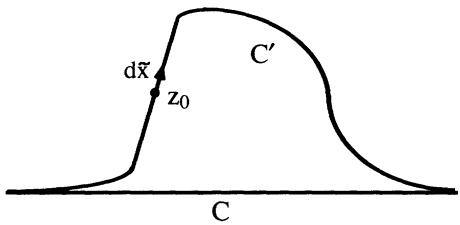
\includegraphics[width=0.5\textwidth]{figE_1.jpg}
\caption{鞍点及其最陡下降路径。}
\label{fig:E.1}
\end{figure}

把积分改写为

\begin{align*}
I ( g ) & = e ^ {- g f ( z _ {0} )} I ' ( g ) ,\\
I ' ( g ) & = \int_ {C '} d z \, \exp \left\{ - g [ f ( z + z _ {0} ) - f ( z _ {0} ) ] \right\} ,
\tag{E.5}
\end{align*}

把 $f(z)$ 在 $z_0$ 附近作 Taylor 展开：

\begin{equation*}
f ( \tilde {x} + z _ {0} ) - f ( z _ {0} ) = \frac {1}{2} f^ {(2)} \tilde {x} ^ {2} + \sum_{n = 3} ^ {\infty} \frac {f^ {(n)}}{n !} \tilde {x} ^ {n}.
\tag{E.6}
\end{equation*}

选取围道 $\tilde{x} \in C'$ 使

\begin{equation*}
\left. f^ {(2)} \tilde {x} ^ {2} \right|_{\tilde {x} \in C '} = \left| f^ {(2)} \tilde {x} ^ {2} \right| \equiv y ^ {2}.
\tag{E.7}
\end{equation*}

$C'$（到二阶）是平稳相位路径：

\begin{equation*}
\operatorname{Im} f ( \tilde {x} + z _ {0} ) = \operatorname{Im} f ( z _ {0} ) + \mathcal {O} ( \tilde {x} ^ {3} ).
\tag{E.8}
\end{equation*}

把 $I'$ 按 $g^{-1}$ 幂次展开：

\begin{align*}
I ' ( g ) & = \sqrt {\frac {2 \pi}{g f^ {(2)}}} \int_{- \infty} ^ {\infty} \frac {dy}{\sqrt {2 \pi}} e ^ {- \frac {1}{2} y ^ {2}}\\
& \quad \times \sum_{m = 0} ^ {\infty} \frac {1}{m !} \left( - \sum_{n = 3} ^ {\infty} \frac {f^ {(n)}}{n ! \, g^ {\frac {n}{2} - 1} \left( f^ {(2)} \right) ^ {\frac {n}{2}}} \, y ^ {n} \right) ^ {m}.
\tag{E.9}
\end{align*}

由对称性，$y$ 的所有奇次幂消失。把被积函数改写为 $y^{2n}$ 的幂级数，系数 $a_{2n}$。Gauss 积分为

\begin{equation*}
\int_{- \infty} ^ {\infty} \frac {dy}{\sqrt {2 \pi}} \, y ^ {2n} e ^ {- \frac {1}{2} y ^ {2}} = 1 \cdot 3 \cdot 5 \dots \left( 2n - 1 \right) = \left( 2n - 1 \right)!! ,
\tag{E.10}
\end{equation*}

由此得

\begin{equation*}
I ' ( g ) = \sqrt {\frac {2 \pi}{g f^ {(2)}}} \left[ 1 + \sum_{n = 1} ^ {\infty} g ^ {- n} a_{2n} \left( 2n - 1 \right)!! \right].
\tag{E.11}
\end{equation*}

存在多个鞍点的情形：

\begin{equation*}
\left. \partial_ {x} \operatorname{Re} f \right|_{z _ {0} ^ {\alpha}} = 0 \, , \quad \alpha = 1, 2, \dots .
\tag{E.12}
\end{equation*}

若鞍点之间的距离远大于 $I'$ 的典型涨落：

\begin{equation*}
\left| z _ {0} ^ {\alpha} - z _ {0} ^ {\alpha '} \right| \gg \frac {1}{\sqrt {g f^ {(2)}}} ,
\tag{E.13}
\end{equation*}

则可以把各鞍点当作独立积分求和：

\begin{equation*}
I ( g ) = \sum_ {\alpha} e ^ {- g f ( z _ {\alpha} )} I _ {\alpha} ' ( g ) ,
\tag{E.14}
\end{equation*}

$I_{\alpha}'$ 是绕 $z_0^\alpha$ 的涨落积分。

把最陡下降展开推广到多维积分是直截了当的。给定积分

\begin{equation*}
I ( g ) = \int \mathcal {D} \mathbf {z} \, e ^ {- g f ( \mathbf {z} )} ,
\tag{E.15}
\end{equation*}

$\mathbf{z} = (z_1, \ldots, z_{\mathcal{N}})$，寻找鞍点

\begin{equation*}
\left. \partial_ {x _ {i}} \operatorname{Re} f \right|_{\mathbf {z} _ {0}} = 0 \, , \quad i = 1, \dots , \mathcal {N}.
\tag{E.16}
\end{equation*}

鞍点 $z_{0}$ 一般是复矢量，它在由 $x_{i}$ 参数化的 $\mathcal{N}$ 条围道上使 $\operatorname{Re}f(\mathbf{z})$ 极小。围道的选取使 $\operatorname{Im}f$ 在鞍点附近为常数。(E.16) 是 $\mathcal{N}$ 个耦合的非线性方程，文献中有许多名称：“鞍点方程”、“经典运动方程”、“平均场方程”等，取决于所论积分与控制其展开的大参数。

$f$ 绕鞍点 $\mathbf{z}_0$ 的二次型定义逆“传播子”$D$：

\begin{equation*}
D _ {i, j} = \frac {1}{2} \left( \partial_{\tilde {x} _ {i}} \partial_{\tilde {x} _ {j}} f \right)_{i, j} ^ {- 1}.
\tag{E.17}
\end{equation*}

$D$ 是 Gauss 系数 $f^{(2)}$ 之逆的推广，描述变量 $\vec{x}$ 中涨落之间的有效相互作用，文献中常称为“RPA 传播子”\footnote{RPA 即“随机相位近似”，例如见 17.2 节。}。

\begin{chapbib}
\item 最陡下降法的简明参考文献：
  G. Arfken, \textit{Mathematical Methods for Physicists} (Academic Press, 1970), 7.4 节。
\end{chapbib}


% 卷末：译者说明
\chapter*{译者说明}
\addcontentsline{toc}{chapter}{译者说明}

本卷系依据 Assa Auerbach 著《Interacting Electrons and Quantum Magnetism》（Springer-Verlag，1994 年初版；本重排本所据扫描件为 1998 年第二次印刷修订版）整理翻译而成，收录原书全部正文：第一至第三部分共十九章，以及第四部分数学附录 A--E。

整理体例如下：

\begin{itemize}[leftmargin=2em, itemsep=2pt]
\item 正文（含全部推导、定理与证明）逐节译为中文；公式、编号、图表号一律保留原书样式，正文引用写作“式 (x.y)”。
\item 人名不译（如 Hubbard、Heisenberg、Néel）；中文学界已有完全定名者使用定名（如海森堡模型、伊辛模型、福克态等）；模型名 t--J、$CP^{N-1}$、SBMFT 等保持原样。
\item 每章末尾的 Exercises 译作“习题”，Bibliography 译作“文献注释”，条目按原文保留。
\item 原书正文脚注全部随文还原为当页脚注；个别原书排印错误（如第 11 章引言“11.2 节”应为 7.1 节、式 (13.39) 后 $\zeta_1$ 的取值）照录并加“原书如此”注。
\item 原书插图由 Dick Codor 绘制，各部扉页插画照录；编号插图共 30 幅，均取自原书扫描件。
\item 原书卷末 Subject Index 按英文页码与英文条目编排，与中文重排本的页码不对应，故本卷不收录；读者可按章检索目录定位主题。
\end{itemize}

\vspace{2em}
\begin{center}
{\kaishu 全书终}
\end{center}


\end{document}
